%!TEX program = xelatex
\documentclass{report}
\usepackage{amsmath}
\numberwithin{equation}{chapter}
\usepackage{amssymb}
\usepackage{sidecap}
\usepackage{caption}
\usepackage{pifont}
\usepackage{graphicx}
\graphicspath{{figure/}}
\usepackage{geometry}
\geometry{a4paper,scale=0.8}
\usepackage{float}
\usepackage{multirow}
\usepackage{titlesec}
\usepackage{verbatim}
\usepackage{subfigure}
\usepackage{color}
\titleformat*{\section}{\LARGE\bfseries}
\titleformat*{\subsection}{\Large\bfseries}
\let\footnotesize\large
\setlength{\parskip}{1em}
\setlength{\parindent}{0pt}
\title{Lecture Notes of Quantum Mechanics}
\author{Translated by Yu Zhu}
%\date{\today}


\begin{document}\Large
\maketitle
\tableofcontents
\listoffigures
%\listoftables
\setcounter{chapter}{7}

%\chapter{Introduction}
%\section{Introduction}
Starting in the 19th century, the physical worldview was based on following theories:
\begin{itemize}
    \item Mechanics (Newton)
    \item Electrodynamics (...., Coulomb, Ampere, Faraday, Maxwell)
    \item Thermodynamics (...., Boltzmann)
\end{itemize}
The existence of atoms/molecules has just been accepted by physicists, the dispute among the chemists was still open. The Avogadro/Loschmidt's number of molecules per mole was found to be N $\sim {10}^{22}-{10}^{24}$
(today N = $6.02\cdot10^{23}$) estimated and for the radius of the H-Atoms/$H_{2}O$ molecules
The estimates ranged from $1 - 2\cdot10^{-8} $cm, ie.
1-2 $\dot{A}$. In the period from about 1900 to 1930 a number of experiments, which were in clear contradiction to the classical worldview. These
experiments seemed to show (and indeed did) that
\begin{center}
(Light-) waves $\to$  are Particles,\\
Particles $\to$  are Waves,
\end{center}
and that quantization of physical quantities such as energy or angular momentum occurs. The explanation of all these experiments by the (new) Quantum mechanics based on the work of Heisenberg, 1925 ($\gets$Bohr, Born, Jordan, Pauli) and his rival Schrodinger, 1926 ($\gets$de Broglie, Einstein) is probably the greatest triumph of physics in the last century. Heisenberg's (abstract) matrix formalism and Schrodinger's (illustrative) wave mechanics turned out to be equivalent (Schrodinger
1926) and formed together with the Copenhagen interpretation
(Heisenberg'sche Unsch arferelation, Bohr, Born, ...) the foundations of
Quantum mechanics as we know it today. In the following we discuss
some key experiments that inspired the development of quantum mechanics
to have.

\section{1900 Planck's law of radiation}
Consider a cavity ($V = L^3$) of temperature T. The classical Rayleigh-Jeans law for the spectral energy density $u(w)$ [Energy/Volume Hz] follows from the counting of the free electromagnetic modes and the fact that classically every fashion carries the energy $k_BT$. One simple argument for counting the modes in volume V is provided by the Application of periodic boundary conditions for the vector potential, $\vec{A}=\sum_{\vec{k}} \vec{A}_{\vec{k}} \exp (i \vec{k} \cdot \vec{r}) \text { with } \vec{k} \cdot \vec{A}_{\vec{k}}=0$ ($\vec{A}$ is transversal) and $\vec{A}_{-\vec{k}}=\vec{A}_{\vec{k}}^{*}$ ($\vec{A}$ is real). Allowed $\vec{k}-$ values are $\vec{k}=(2 \pi / L) \vec{n}$ with $n_i$ all and we get the Number of dN modes in the interval $[k, k+ dk]$ (factor 2 for two transversal Directions, factor 2 for $\vec{A}_{\vec{k}}$ complex, factor 1/2 for $\vec{A}$ real)
\begin{equation} \label{0.1}
d N=2 \cdot 2 \cdot \frac{1}{2} \cdot \frac{4 \pi k^{2}}{(2 \pi / L)^{3}} d k
\end{equation}
If you want to find the physically correct modes you have to do more work. We take an ideal metallic cavity at dimension $L^2d$ ($d = L $ at the end) and TE (transversal electrical) and TM (transversal
magnetic) modes (see electrodynamics lecture or J. D. Jackson,
Classical Electrodynamics),
\begin{equation}
\begin{array}{c}{\mathrm{TE}: H_{z} \propto \cos (m \pi x / L) \cos (n \pi y / L) \sin (p \pi z / d)} \\ {m, n \mbox  { for all, not both }=0, p \neq 0 \mbox{ for all}}\end{array}
\end{equation}
\begin{equation}
\begin{array}{c}{\mathrm{TM}: E_{z} \propto \sin (m \pi x / L) \sin (n \pi y / L) \cos (p \pi z / d)} \\ {m, n \neq 0 \mbox{ for all}, p \mbox  { for all }}\end{array}
\end{equation}
%公式0.2,0.3
The components $\vec{H}_{\bot}$ and $\vec{E}_{\bot}$ follow from $\nabla_{\bot}H_z$ and $\nabla_{\bot}E_z$. Then counting the allowed values for $m,n,p$ (with $ d = L$) then yields $dN = (1/8)\cdot 2 \cdot 4\pi k^2 / (\pi/L)^3 dk$, in agreement with (Formula 0.1) (factor 1/8 for one octant, factor 2 for TE and TM modes).
%图1
\begin{figure}[ht]
    \centering
    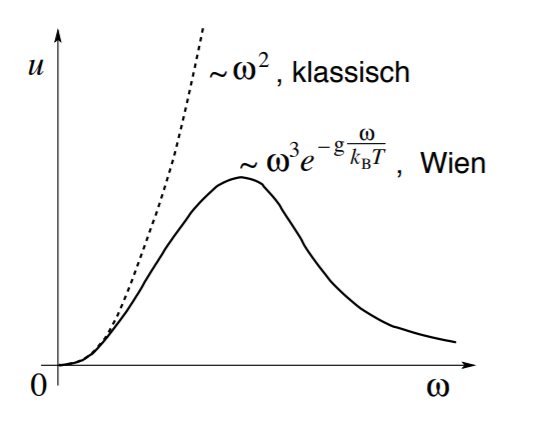
\includegraphics[scale=1]{1.PNG}
    \captionsetup{font={Large}}
    \caption{Spectral energy density $u(w)$. The classically unlimited energy density (dotted) saturates in reality (extended) and falls exponentially to zero at high energies (Wien and Planck's law of radiation).}
    \label{fig:1}
\end{figure}
In thermodynamic equilibrium at the temperature T, each mode carries an energy $k_BT$ ($k_B = 0.8617 10^{-4} eV/K$) designates the Boltzmann
Constant) and with the dispersion $w = ck (c = 2.998 10^8 m/s$, the speed of light). For light, the spectral energy density results:
\\\begin{equation}
u(\omega) d \omega=\frac{k_{\mathrm{B}} T}{\pi^{2} c^{3}} \omega^{2} d \omega
\end{equation}

%公式0.4
This results in the ultraviolet catastrophe:
\begin{equation}
\int_{0}^{\infty} d \omega u(\omega)=\infty
\end{equation}
%公式0.5
However, experiments and empirical analyzes show (Vienna) that
\begin{equation}
u(\omega) \sim\left\{\begin{array}{ll}{\omega^{2},} & {\omega \rightarrow 0} \\ {\omega^{3} e^{-g \omega / k_{\mathrm{B}} T},} & {\omega \rightarrow \infty}\end{array}\right.
\end{equation}
%公式0.6
as shown in Figure 1. The constant $g$ has the dimension energy times, which gives an effect; you determine them via comparison with experiments. Find Planck's Law of Radiation based on the hypothesis that matter only radiation in quanta of $\hbar w$ releases;
Under this assumption we find the new expression for the spectral energy density
\begin{equation}
u(\omega)=\frac{\hbar}{\pi^{2} c^{3}} \frac{\omega^{3}}{e^{\hbar \omega / k_{\mathrm{B}} T}-1}
\end{equation}
with
\begin{equation}
 \hbar=6.58210^{-16} e \mathrm{Vs}=1.05510^{-34} \mathrm{Js}
\end{equation}
%公式0.7,0.8
The comparison with the experiment gives a first indication of the quantization of the radiation field.(Modern formulation: the mode with$w = ck$ is using a number of quanta $\langle n\rangle$)


%PAGE 4
\section{1905 Photoelectric effect(Einstein)}
Becomes a (metallic) upper ache by light ((circle) frequency $w$, visible or UV) (Hertz, Lenard) you find an upper limit
\begin{equation}
E_{\mathrm{kin}}=\frac{m v^{2}}{2}=\hbar \omega-W
\end{equation}
%公式0.10
for the kinetic energy of electrons ($\gets$ J.J. Thompson, 1897, Elektronen as constituents of the atoms: J.J. Thompson $\sim$1899). $W$ is the work function, with a value in the size order $eV$. Classic would expect another result: the intensity of the radiation is increased by their energy flux density $\vec{S} = (c/4\pi)\vec{E}\times \vec{H}$ characterized. The continuous absorption of this radiation can be expected that $i$) no upper bound
for the kinetic energy $E_{kin}$ exists, $ii$) no lower bound for $w$ occurs, and $ iii$) a delayed emission at low intensity (proportional
to the energy density $(E^2 + H^2) /8\pi$) occurs. Instead, you find as shown in Figure 2, the photocurrent starts immediately when $\hbar w > W$
(lower bound for $w$) and $E_{kin}$ is limited. It can be concluded that light consists of photons (energy quanta of energy $\hbar w$). Spater de Broglie and Compton showed that the light waves correspond to particles with\\
\begin{equation}
\begin{array}{l}{\mbox { Impulse: } \vec{p}=\hbar \vec{k}, \quad \omega=c k} \\ {\mbox  { Energy : } E=\hbar \omega} \\ {\mbox  { Foursome pulse: }\left(\begin{array}{c}{E / c} \\ {\vec{p}}\end{array}\right)=\hbar\left(\begin{array}{c}{k} \\ {\vec{k}}\end{array}\right)}\end{array}
\end{equation}
%公式0.11
occupied by the given
\\
\begin{equation}
    \langle n(\omega)\rangle \sim \frac{\sum_{n} n e^{-\beta n \hbar \omega}}{\sum_{n} e^{-\beta n \hbar \omega}}=\left.\left(1-e^{-y}\right)\left(-\partial_{y}\right)\left(1-e^{-y}\right)^{-1}\right|_{y=\beta \hbar \omega}=\frac{1}{e^{\hbar \omega / k_{\mathrm{B}} T}-1}
\end{equation}\\
%公式0.9 
with $\beta = 1/k_BT$. Each mode then carries an energy $\hbar w\langle n(w)\rangle$ to the energy density of the
radiation field at. For small energies $\hbar w <k_BT$ can be the exponential function in $\langle n(w)\rangle$ develop and you will continue to find the contribution $\hbar w\langle n(w)\rangle \approx k_BT$, during modes with $\hbar w > k_BT$ contributes little exponentially. Task: Compare $\langle E\rangle_{classical}$, and $\langle E\rangle_{qm}$.

%Page 5
%图2
\begin{figure}[ht]
    \centering
    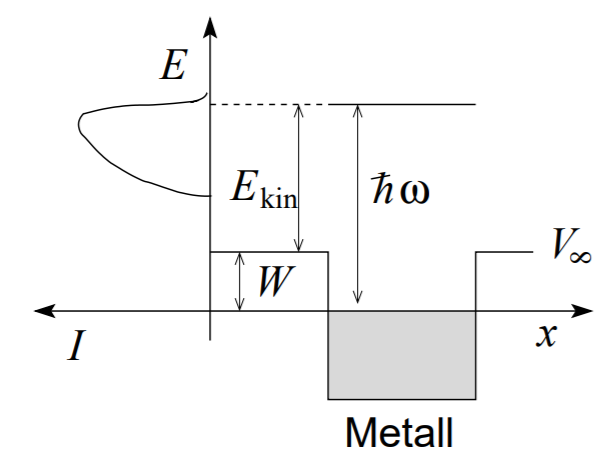
\includegraphics[scale=1]{2.PNG}
    \captionsetup{font={Large}}
    \caption{Photons of energy $\hbar w$ strike electrons from a metal. The intensity (left) of the emitted electrons is limited by the band edge (bottom) and by the Fermi energy of the metallic electrons (top).}
    \label{fig:2}
\end{figure}
\section{1907 Special Warmth of the Festival (Einstein)}
The quantization of the excitations (phonons) in the solid state is in the treatment of the cavity radiation/Planck's law of radiation similar;Differences are in the spectrum (dispersion) and in the finite number of modes (finite number of atoms, finite grid instead of continuous vacuum). We will not go back to it.

\section{1913 Bohr quantization of the atom}
Starting point is the Rutherford atom with small, positively charged core (extension $\sim10^{-13} - 10^{-12}$ cm) orbited by (negatively charged) electrons (J.J. Thompson, 1899). The formula $v=R(1/n^2 - 1/m^2), R = \text{Rydberg Constant}, m, n$ for all, for the Balmer series describes the frequencies the observed spectral lines. Classically, the electron moves in a circular path and is thus accelerated.\\
Due to this orbital motion, the atom emits energy off and the electron should (with emission of continuous radiation) to the core. Bohr postulates that atom exists only in stationary or quantum states of well-defined energy. The sharp spectral lines are then the consequence of transitions between these states.
\\
\begin{equation}
\hbar \omega=\left|E_{f}-E_{i}\right|, \quad \begin{array}{ll}{\text { Absorption : }} & {E_{i}<E_{f}} \\ {\text { Emission: }} & {E_{i}>E_{f}}\end{array}
\end{equation}\\
%公式0.12
where $i,f$ for the $i$ initial, $f$ final state. The ground state $E_0 =min (E_i)$ is stable. For the hydrogen atom applies \\
\begin{equation}
E_{n}=-\hbar \frac{2 \pi R}{n^{2}}, \quad n=1,2,3, \ldots
\end{equation}\\
%公式0.13
from which the Balmer formula results.

\section{1914 Franck-Hertz experiment}
The experiment, see Figure  3, underlines the existence of discrete energy levels in atoms. The structure (peaks) in the observed current
%图3
\begin{figure}[ht]
    \centering
    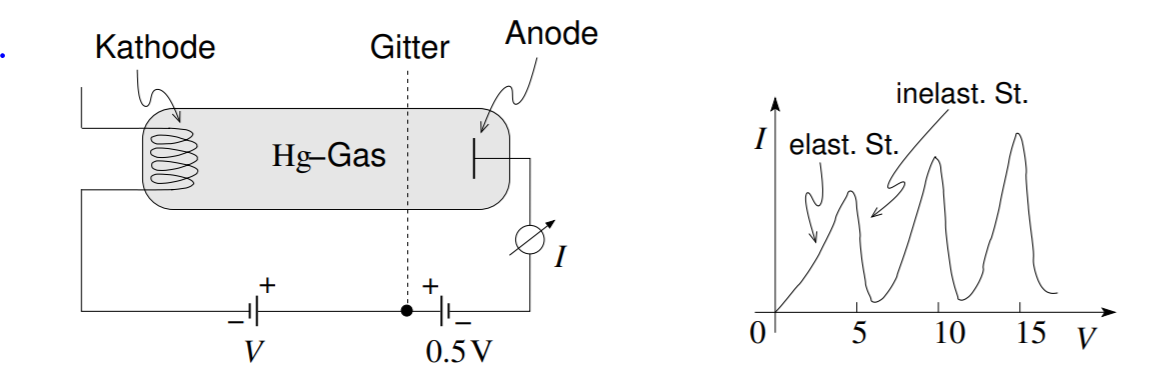
\includegraphics[scale=1]{3.PNG}
    \captionsetup{font={Large}}
    \caption{Electrons accelerated by an electric potential hit Hg atoms. Inelastic shocks transfer the atoms into high-energy excited states, which decay under the emission of electromagnetic radiation.}
    \label{fig:3}
\end{figure}
versus voltage characteristic is interpreted as follows: electrons take in the potential $V$ kinetic energy, which they release to the same through inelastic collision with the Hg atoms. The atoms are from the ground state with energy $E_0$ in an excited state with energy $E_n, E_n - E_0 \approx 5 eV$ lifted. The stopped electrons reach the anode no more and there are peaks in $I (V)$; the atoms are falling emission of radiation back to the ground state.

\section{1922 Stern-Gerlach experiment}
Paramagnetic atoms with magnetic moment $\vec{\mu} = \mu_0 \vec{L}, \vec{L}$ the angular momentum, are exposed to an inhomogeneous magnetic field $\vec{B}$ and their distraction is measured. Classically, the following behavior is expected:
%图4
\begin{figure}[ht]
    \centering
    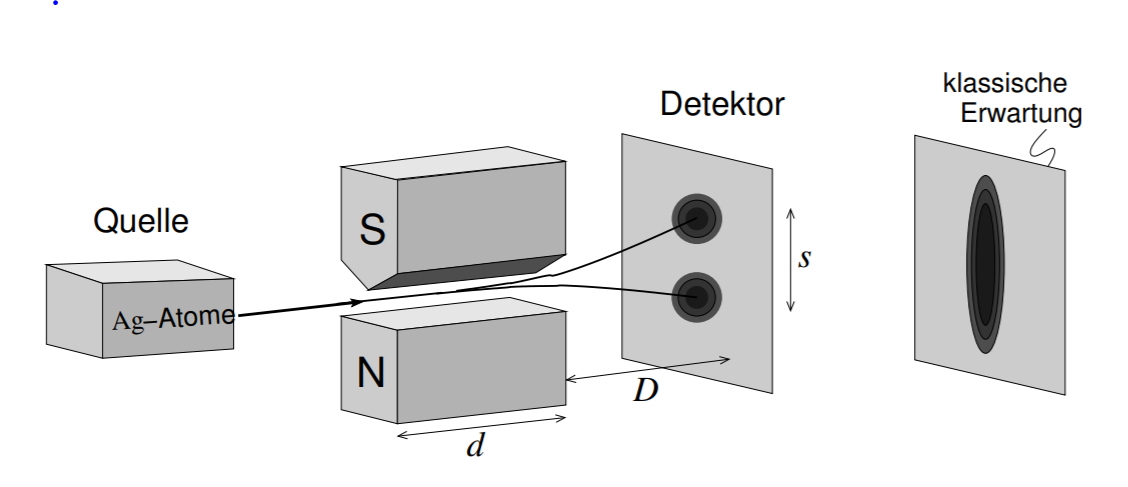
\includegraphics[scale=1]{4.PNG}
    \captionsetup{font={Large}}
    \caption{Paramagnetic atoms with magnetic moment $\vec{\mu}=\mu_0 \vec{L}$= angular momentum and (thermal) energy $E = mv^2/2 \approx k_BT$ are deflected in an inhomogeneous magnetic field. Discrete spots are observed at the detector instead of the traditionally expected continuous distribution.}
    \label{fig:4}
\end{figure}
the energy in the magnetic field $E_{magn}=-\vec{\mu}\cdot \vec{B}$ yields the force $\vec{F}=\bigtriangledown(\vec{\mu}\cdot\vec{B})$. Here is $F_z=\mu_z\partial_zB$, for example, and that's the reason for the distraction on the screen
$s=(\mu_z\partial_zBd/2k_BT)(d/2+D)$. Since (classical) the angular momentum $L_z$ along $z$ is continuously distributed, it would be a continuous distribution of
atoms along $z$ direction, see Figure  4, in contradiction to the factual observed quantized results with discrete patches. Consequently, the angular momentum of atoms quantized.

\section{1923/25 Compton Effect (Compton and Debye)}
In this experiment, light rays are scattered by electrons, the geometry sketched in Figure  5.
Classically, the following results are expected: a continuous pulse transfer from the radiation field to the electron (the radiation pressure causes the momentum $p_e$ of the electron to grow continuously with the irradiation time); all electrons are accelerated equally; the absorption and re-emission of radiation by the electron takes place in (momentary)
Resting system of the electron at the same wavelength. The Doppler effect then produces a (angle-dependent) wavelength shift $\triangle \lambda $ ($\lambda$ is the wavelength of the incident beam),\\
\begin{equation}
\Delta \lambda=2 \lambda \frac{c p_{\mathrm{e}}}{E_{\mathrm{e}}-c p_{\mathrm{e}}} \sin ^{2} \frac{\theta}{2}, \quad \vartheta=0, \quad E_{\mathrm{e}}^{2}=m_{\mathrm{e}}^{2} c^{4}+p_{\mathrm{e}}^{2} c^{2}
\end{equation}\\
%公式0.14
In fact, however, you find the shift
\\
\begin{equation}
\Delta \lambda=4 \pi \frac{\hbar}{m_{\mathrm{e}} c} \sin ^{2} \frac{\theta}{2}
\end{equation}\\
%公式0.15
with the new parameter $\hbar/m_ec= 3.86\times10^{-11}$ cm, the Compton Wavelength of the electron. Also, one notices that not all electrons accelerated simultaneously and evenly: only those electrons which absorb a photon, have a pulse $p_e \neq 0$ and also
this pulse varies discretely. These results indicate that the light is in the scattering process corresponds to a particle, although the light clearly has wave character, comparing to other experiments with light, e.g. the Double-slit experiment or the action on crystals (von Laue, 1912). The experiment thus points to a particle/wave duality for the radiation.
%图5
\begin{figure}[ht]
    \centering
    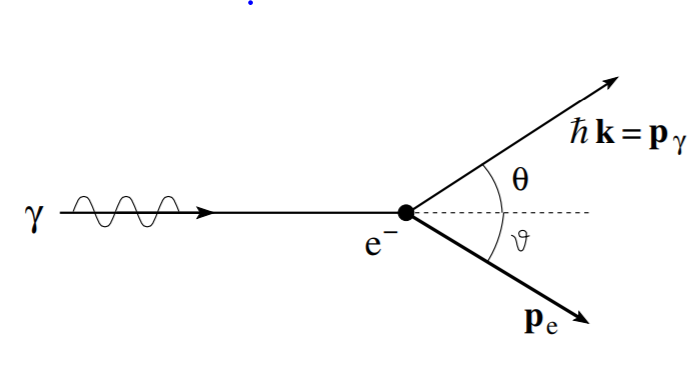
\includegraphics[scale=1]{5.PNG}
    \captionsetup{font={Large}}
    \caption{X-rays (photons) strike a resting electron $e^-$ and are scattered.}
    \label{fig:5}
\end{figure}
The assumption that the scattering process as particles-particles (i.e., photon-electron) scattering with momentum and energy conservation (4-invariant)
can lead to the correct result (0.15): the four-momentum remains in the scattering process,
\\
\begin{equation}
\begin{array}{l}{\text { initial: }\left(\begin{array}{c}{\hbar k} \\ {\hbar \vec{k}}\end{array}\right)+\left(\begin{array}{c}{m_{\mathrm{e}} c} \\ {0}\end{array}\right), 
\quad \text { final: }\left(\begin{array}{c}{\hbar k^{\prime}} \\ {\hbar \overrightarrow{k^{\prime}}}\end{array}\right)+\left(\begin{array}{c}{\sqrt{p_{\mathrm{e}}^{2}+m_{\mathrm{e}}^{2} c^{2}}} \\ {\hbar \overrightarrow{k^{\prime}}}\end{array}\right)%+\left(\begin{array}{c}{\sqrt{p_{\mathrm{e}}^{2}+m_{\mathrm{e}}^{2} c^{2}}} \\ {\overrightarrow{p_{\mathrm{e}}}}\end{array}\right)
} 
\\ {\left(\begin{array}{c}{\hbar\left(k-k^{\prime}\right)+m_{\mathrm{e}} c} \\ {\hbar\left(\vec{k}-\vec{k}^{\prime}\right)}\end{array}\right)=\left(\begin{array}{c}{\sqrt{p_{\mathrm{e}}^{2}+m_{\mathrm{e}}^{2} c^{2}}} \\ {\vec{p}_{\mathrm{e}}}\end{array}\right)}\end{array}
\end{equation}
%公式0.16,
and the four-squares product $a^{\mu}a_{mu}=a^0a_0-\vec{a}\cdot\vec{a}$ are
\begin{equation}
k-k^{\prime}=\frac{\hbar}{m_{\mathrm{e}} c} k k^{\prime}(1-\cos \theta)
\end{equation}
%公式17
The result (0.15) then follows with the assumption $k = 2\pi/\lambda$. The experiment attests to the light a particle character
\\
\begin{equation}
\begin{aligned} E &=\hbar \omega \\ \vec{p}_{\gamma} &=\hbar \vec{k}=\vec{p}, \quad \quad P^{\mu}=\left(\begin{array}{c}{E / c} \\ {\vec{p}}\end{array}\right)=\hbar\left(\begin{array}{c}{k} \\ {\vec{k}}\end{array}\right) \\ \vec{p} / p &=\text { propagation } \\ \omega &=c k \end{aligned}
\end{equation}
%公式0.18

\section{1923 de Broglie hypothesis}
Matter and radiation behave the same (universal) and show both wave and particle character,
\begin{equation}
\begin{array}{l}{\text { Wave } \longrightarrow \text { Particle } \stackrel{\text { DeB }}{\rightarrow} \text { Wave }} \\ {\qquad(h=2 \pi \hbar)}\end{array}
\end{equation}\\
%公式0.19
That a wave behaves like a particle follows from the photoelectric effect and the Compton scatter. De Broglie rearranges the particle with momentum$ p$
, a wave with wavelength $\lambda=h/p$ too.

\section{1923 Bohr's correspondence principle}
Classical theory is macroscopic and special in all (for example in the description of electrons in static electromagnetic field) also microscopically correct. On the other hand, the classical theory fails when quantum disciplines become relevant. The quantum theory must reproduce the results of classical theory in the limit of large quantum numbers(corresponding to small quantum discontinuity). Consequently, there must be a formal analogy between quantum theory and classical theory. These arguments form the basis for the correspondence principle. \\\\
As an example, consider the Bohr atom with the energies $E_n=hR/n^2$, see Figure  6. R is an unknown proportionality constant. The classical analogue is the Kepler problem with the gravitational potential
replaced by the electrical potential $-e^2/r$. The Kepler law for the rotational frequency $v(E) = 1/T$, $T$ the orbital period, $E$, the energy of the
%PAGE 10
classic elliptical orbit, is (transferred to the electronic potential)
\begin{equation}
\nu=\frac{1}{\pi e^{2}}\left(\frac{2|E|^{3}}{m}\right)^{1 / 2}
\end{equation}
%公式0.20
On the other hand, a quantum mechanical view of the spectrum results at high energies the (energy-dependent) fundamental frequency
\begin{equation}
\nu\left(E_{n}\right)=\frac{E_{n+1}-E_{n}}{h} \approx \frac{1}{h} \frac{d E_{n}}{d n}(\Delta n=1)=\frac{2 R}{n^{3}}=2\left(\frac{\left|E_{n}\right|^{3}}{R h^{3}}\right)^{1 / 2}
\end{equation}
%公式0.21
where we have used the dependency $E_n = hR/n^2$. The relevant frequencies in the radiation at high energies are then given by $[E_{n+\triangle n}-E_n=v_{\triangle n}(E)=\triangle n v(E)]$, provided that $\triangle n/n \ll 1$ satisfied.
%图6
\begin{figure}[ht]
    \begin{minipage}{0.5\textwidth}
        \centering
        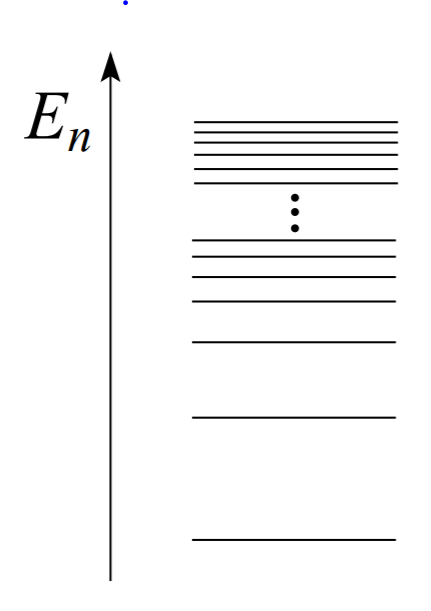
\includegraphics[scale=1]{6.PNG}
    \end{minipage}
    \begin{minipage}{0.5\textwidth}
        \captionsetup{font={Large}}
        \caption{Discrete spectrum in Bohr's atomic model. The correspondence principle can be applied to high excitation energies $E_n$ with $n\gg 1$, where the spectrum is quasi-continuous.}
    \end{minipage}
    \label{fig:6}
\end{figure}
From the correspondence between the Kepler problem (0.20) and the quantum mechanical problem (0.21) we get an expression for the constant $R$\\
\begin{equation}
\begin{aligned} \nu_{\mathrm{Kep}} &=\frac{1}{\pi e^{2}}\left(\frac{2|E|^{3}}{m}\right)^{1 / 2}=2\left(\frac{|E|^{3}}{R h^{3}}\right)^{1 / 2}=\nu_{q} \\ & \rightarrow R=\frac{2 \pi^{2} m e^{4}}{h^{3}}, \quad E_{n}=-\frac{m e^{4}}{2 \hbar^{2}} \frac{1}{n^{2}}=-\frac{13.6 \mathrm{eV}}{n^{2}} \end{aligned}
\end{equation}\\
%公式0.22
We briefly check the dimensional correctness of the result: the ground state is characterized by the potential and kinetic energies $E_{pot}\approx -e^2/r$ and $E_{kin} = p^2/2m \approx \hbar^2\pi^2/2mr^2$, where we
%PAGE 11
have used the blurring relation in the form $p\cdot r\sim\pi\hbar$. Put
we $E_{kin}\approx -E_{pot}$ (virial theorem), we get $r \approx \hbar^2\pi^2/2me^2$ and
$E \approx -2me^4/\pi^2\hbar^2$, which is a factor $4/\pi^2\approx 0.4$ .

\section{1925 Matrix Mechanics (Heisenberg)}
See detailed discussion later.
\section{1926 Wave mechanics (Schrodinger)}
See detailed discussion later.
\section{1927 Davisson and Germer experiment}
We consider the scattering experiment analogous to the Laue experiment but with particles. The reflection of electrons from a crystal survey yields `von Laue' reflection as sketched in Figure  7. 
%图7
\begin{figure}[ht]
    \centering
    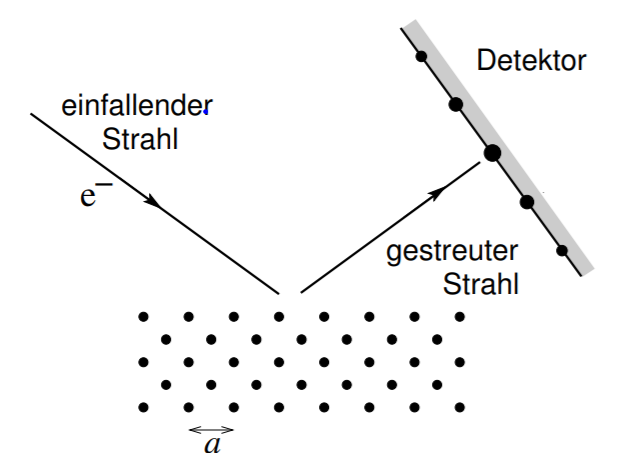
\includegraphics[scale=1]{7.PNG}
    \captionsetup{font={Large}}
    \caption{Scattering of electrons on a crystal surface.}
    \label{fig:7}
\end{figure}
The needed wavelength and energy of the electrons are obtained from the de Broglie Relationship (use that $\hbar\cdot \hbar=6.58\times 10^{-16}eVs \cdot 1.055\times 10^{-34}Js$)
\\\begin{equation}
\lambda=\frac{2 \pi \hbar}{p}=\frac{2 \pi \hbar}{\sqrt{2 m E}}=\frac{12.2 \mathrm{A}}{\sqrt{E[\mathrm{eV}]}}
\end{equation}
\\
%公式0.23
The lattice constant $a \sim5 \overset{\circ}{A} $leads to an energy $E$ of a few $eV$; This is just the typical energy scale of the electrons in the crystal (The electrons in the crystal are compatible with a crystal structure of length scale $a$).\\\\
%PAGE 12
Conversely, the structure of the Laue interference image confirms the validity of the De Broglie relation $\lambda = h/p$ (the interference pattern gives a value of the compatible $\lambda$ with the energy $E$ of the scattered electrons).
\section{1913-1927 Bohr-Sommerfeld Quantization and `old' quantum mechanics}
The correspondence principle and the Bohr quantization lead to a selection criterion for classical orbits permitted in quantum mechanics: select those orbits which satisfy a quantization condition (the criterion works for periodic orbits). This gives us the transition from continuous to quantized results. The desired quantization must have something to do with Planck's quantum effect. Dimensionally, $[h]$ = effect, so the effect of the orbit is to be quantized. Returning to Lagrangian mechanics, a mechanical problem is defined by the coordinate $q$ and the Lagrange function $\mathcal{L}$. The conjugate momentum is given as the derivative $p = \partial \mathcal{L}/\partial q$, and the effect of a trajectory is given by the time integral
\begin{equation}
\mathcal{S}=\oint d t \mathcal{L}=\oint d q p-E \oint d t
\end{equation}
%公式0.24
where we have separated the district. The latter we quantify according to
\begin{equation}
\oint d q p=n h
\end{equation}
%公式0.25
with $n \in N$. In the example the hydrogen atoms become the radial and azimuthal ones track shares quantized,$\oint d r p_{r}=k h$and$\oint d \varphi p_{\varphi}=l h$. We choose
a fixed orbital plane; with $\mathcal{L}=(m / 2)\left[\dot{r}^{2}+(r \dot{\varphi})^{2}\right]+e^{2} / r$ follows $p_{r}=\partial_{i} \mathcal{L}=m \dot{r} $ $p_{\varphi}=\partial_{\dot{\varphi}} \mathcal{L}=m r^{2} \dot{\varphi}=L $ with the obtained angular momentum $L=\hbar l$.
The second integral $0>E=H=p_{r} \dot{r}+p_{\varphi} \dot{\varphi}-\mathcal{L}=p_{r}^{2} / 2 m+L^{2} / m r^{2}-e^{2} / r $ together with $2 \int_{r_{\text {min }}}^{r_{\text {max }}} d r p_{r}=k h$ gives the second condition
\\
\begin{equation}
\left(\frac{2 \pi^{2} m e^{4}}{|E|}\right)^{1 / 2}-l h=k h
\end{equation}
\\
%公式0.26
and thus $E_n=-me^4/2\hbar^2n^2$  with $n = l + k$. The classic orbits are ellipses with eccentricity at
$\sqrt{1+2 E L^{2} / m e^{4}}=\sqrt{1+l^{2} / n^{2}}$ for $l = n$
a circular path (Bohr 1913); for $ 0 <l <n$, ellipses result
%PAGE13
(Sommerfeld). The case $ l = 0 $ is nontrivial, see later or Migdal; the Degeneracy factor for $E_n$ is $n + 1$ (until now, it will have to be correct). If we release the plane of the orbit, we get the quantization requirement for the $z$-component of the angular momentum,$\oint d \varphi L_{z}=m h$ and so on $L_z = m\hbar$. The magnetic quantum number assumes values ​​$-l \leq m \leq l$ and gives the additional degeneracy factor $2l + 1$(The Langer-correction replaces $L^2\to l(l+1)\hbar^2\to (l+1/2)^2\hbar^2$(quasi-classical approximation); in the same frame is $k\to k+2\cdot 1/4$ to replace, a consequence of reexpression at the local linear potential, see chapter 10 about quasiclassical methods or migdal.)

\section{1927 Heisenbergsche Unsch arferelation}
Together with the matrix or wave mechanics as well as the Copenhagen interpretation of quantum mechanics results in the `new’ quantum mechanics. Let $p$ and $q$ be conjugate variables, e.g. $p_x$ and $x$, $L_z $ and $\varphi$, $E$and $t$. Then a simultaneous determination of $p$ and $q$ is only a blur $\triangle p\cdot \triangle q \gtrsim \hbar$. In particular, if $q$ is known then $\triangle q = 0$ and thus $\triangle p = \infty$, i.e. $p$ is completely undetermined and vice versa. The blushing relation yields the break with the causality of classical physics: classically, the initial conditions and the dynamic laws (e.g., $\dot{p}=-\partial_q{H}$, $\dot{q}=\partial_p{H}$) set the lanes for all times. According to the Heisenberg Uncertainty Principle (HUP), one of the prerequisites of determinism is not met: the initial conditions can not be set sharply and thus we lose the classical causality (Einstein's objection to the completeness of QM on this `defect' of theory). However, it is important (and correct) that a consistent interpretation of QM can only be achieved with the help of Heisenberg's Uncertainty interpretation (HUR) (see later). The classic experiment (thought experiment, quoted by Heisenberg (wrong) and corrected by Bohr) is the on-line microscope (see Figure  8) for observing an electron: according to wave optics, the resolution of a lens can reach:
\begin{equation}
\Delta x=\frac{\lambda}{2 \sin \theta}
\end{equation}
%公式0.27
The quantum of light ($\gamma$) must reach the lens. The maximum and minimum momentum transfer to the electron ($e^-$) is $p_{max} = p + h sin\theta/\lambda$ and $p_{min}=p - h sin\theta/\lambda$
%PAGE 14
(the scattering process is approximated as elastic), from which an impulse is transmitted:
\\
\begin{equation}
\Delta x \Delta p \sim h
\end{equation}\\
%公式0.28
A more rigorous derivation of the HUR will follow later. Hereinafter
%图8
\begin{figure}[ht]
    \begin{minipage}{0.5\textwidth}
        \centering
        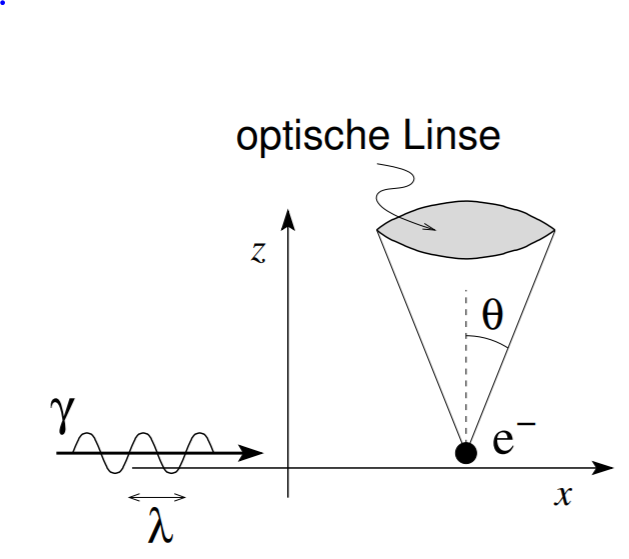
\includegraphics[scale=0.8]{8.PNG}
    \end{minipage}
    \begin{minipage}{0.5\textwidth}
        \captionsetup{font={Large}}
        \caption{X-ray microscope for observation of an electron (thought experiment).}
    \end{minipage}
    \label{fig:8}
\end{figure}
we build the Schrodinger wave mechanics from similar thought experiments
on (see, e.g., Feymann \& Hibbs).


%\chapter{Wave mechanics}
\section{Double-slit experiment}
Material for this chapter can be found in the book by Feynman and Hibbs. The experimental setup is outlined in Figure 1.1: a source emits particles (electrons, photons, ...) which impinge on a double-slit screen. The particles propagating through the two columns are registered with a suitable detector.
%图1.1
\begin{figure}[ht]
    \centering
    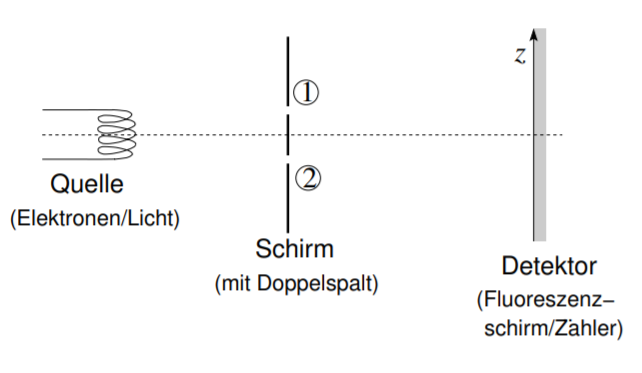
\includegraphics[scale=1]{1_1.PNG}
    \captionsetup{font={Large}}
    \caption{The double-slit experiment: those emitted by the source particles/waves hit a screen with two overlays columns and are analyzed in the detector.}
    \label{fig:1.1}
\end{figure}
\\
The result of the measurement is shown in Figure 1.2 where I = intensity, in $[I]$ = number of particles/s is measured. For a gap (without diffraction), the result for waves and particles looks the same according to classical expectation (see $I_1$ and $I_2$). If both slots are used, one expects (classical) different results, $I_w$ for waves and $I_k$ for particles. However, the experimental result of the double-slit experiment with particles again shows an interference pattern in the intensity, which leads to the conclusion
%PAGE 16
to draw is that the particles propagate like waves.
%图1.2
\begin{figure}[ht]
    \centering
    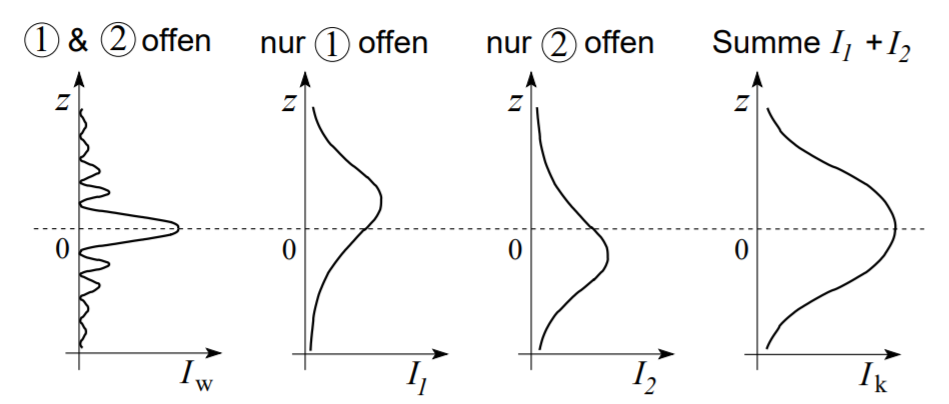
\includegraphics[scale=1]{1_2.PNG}
    \captionsetup{font={Large}}
    \caption{Left: the intensity at $I_w$ is the classically expected interference pattern for waves. The same result is found for the experiment with particles. Right: the intensity $I_k$ is the classically expected result for particles, but is not observed. The conclusion from the experiment is that particles propagate like waves.}
    \label{fig:1.2}
\end{figure}
Also with the detection one finds an unexpected result: becomes classical expected a discrete detection of particles. In contrast, one expects
classic for the intensity of waves a continuous result. The experiment also shows discrete events for the detection of waves, see. Figure  1.3.
%PAGE17
%图1.3
\begin{figure}[ht]
    \centering
    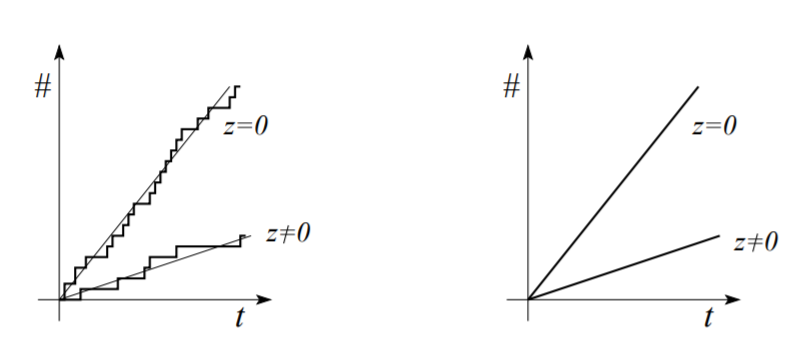
\includegraphics[scale=1]{1_3.PNG}
    \captionsetup{font={Large}}
    \caption{Left: Discrete detection is expected for classical particles. The same finding is obtained for the detection of waves. Right: Continuous detection is expected for waves but is not observed experimentally. One concludes that waves are detected like particles.}
    \label{fig:1.3}
\end{figure}
\\ \\
In summary, the following conclusions are drawn from the experimental findings:
%流程图
in the following we want to formalize this finding. Were we the double-slit experiment classically interpreted, the particle would either have to \ding{172} or \ding{173} happen. Let us denote $P_i(z), i = 1, 2$, as (relative) probability
%PAGE 18
for passage of particles through columns 1 or 2 and subsequent ones detection in $z$ would have been done in open \ding{172} and \ding{173} classical result
\\
\begin{equation}
P(z)=\sum_{i} P_{i}(z) \quad \text { (particle) }
\end{equation}
%公式1.1
expect. On the other hand, for waves we would have an amplitude $\Phi_i(z)$ kidney and the (relative) probability $w$ are then given by
$P_i(z)=| \Phi_i(z) |^2$ if only gap
\textcircled{i} is. If, on the other hand, the columns \ding{172} and \ding{173}, so one expects interference according to
\\
\begin{equation}
P(z)=\left|\sum_{i} \Phi_{i}(z)\right|^{2} \quad \text { (Wellen) }
\end{equation}\\
%公式1.2
The experiment gives the result that the particles are the same probability distribution $P (z)$ as the waves generate, therefore must it is also possible to assign a probability amplitude $\Phi_i (z) \in C$ to the particles and how waves demand the validity of the superposition principle. The problem now arises that one is under a particle, at least according to our perception, always presents a small body, but then either through the gap \ding{172} or \ding{173} the gap to the detector arrives. This contradiction motivates an extension of the experiment in that one measures by what gap the particle to detector arrives, see Figure  1.4.
%图1.4
\begin{figure}[ht]
    \centering
    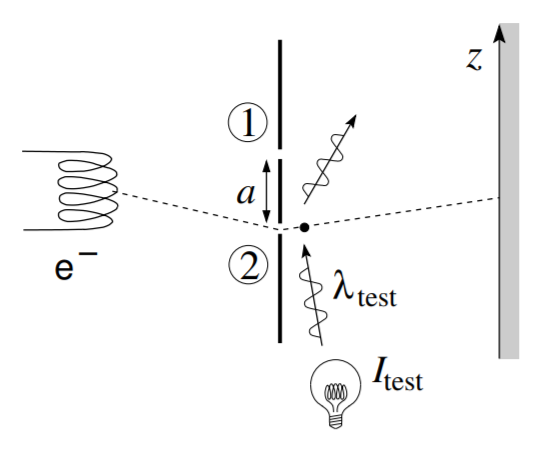
\includegraphics[scale=1]{1_4.PNG}
    \captionsetup{font={Large}}
    \caption{Double slit experiment with detection: Light emitted by the lamp should show the passage of the particle through the gap \ding{173}.}
    \label{fig:1.4}
\end{figure}
\\ \\So we're counting a particle, whenever it's through gap \ding{173}, that is, it must apply now that
\\
\begin{equation}
P=P_{1}+P_{2}
\end{equation}\\
%公式1.3
%PAGE19
is. In fact, this expectation agrees with the result of the experiment. Apparently there is a paradoxical situation here.\\
Next, we minimize the problem by testing with the lamp by reducing the intensity, $I_{test}\to 0$. Once $I_{test}$ is so small that Do not scatter the individual photons at each electron (see Comptoneekt) $P = P1 + P2$ in $P = | \Sigma_i \Phi_i|^2$ about. On the other hand, we can minimize the problem with the test by setting the wavelength of the test Light up, $\lambda_{test}\to \infty$(It does not matter whether we are actually interested in the measurement result or not, it's all about having the measurement results in principle by the lamp behind the double slit the passage of the particles is detected.). Once $\lambda_{test}$ is so large that the distance a is not can be solved more, $P = P1 + P2$ in $P = | \Sigma_i \Phi_i|^2$. If so at least in principle we know whether the particle is now via \ding{172} or \ding{173} to the detector we get $P = \Sigma_i P_i$ otherwise $P = | \Sigma_i \Phi_i|^2$.\\
An experiment that gives the information about the particle taken by the particle path returns (`which path detection'), so it locates the original experiment so strong that the interference is destroyed [see also E. Buks, R. Schuster, M. Heiblum, D. Malahu and V. Umansky, Nature 391, 871 (1998)]. This is a direct manifestation of Heisenberg's principle of blurring. This principle guarantees the consistency of the approach $P = | \Sigma_i \Phi_i|^2$ for propagation the particles; as long as the principle of blur applies, there is no paradox. Till today, all experiments are in harmony with the principle of blur. For a better understanding/proof we will consider a new experiment, whose structure is shown in Figure  1.5.\\
In experiment the spreader (here a screen with a double slit) becomes so set up an electron which passes through the gap \ding{172} i.e., a deflection $\delta z> 0$, one through the gap \ding{173}, a shift $\delta z <0$ is generated. Particles with momentum $p$ generate an interference pattern with $d$ given by ($p = h/ \lambda$, see Figure  1.5)
\\\begin{equation}
\frac{\lambda}{a} \sim \frac{d}{l}
\end{equation}
\\
%公式1.4
The momentum difference $\delta p_z = | p_z^{\ding{172}}$ for particles, which by \ding{172} or \ding{173}, is $\delta p_z \sim pa/l=h/d$. Let's see if choosing the way \ding{172} or \ding{173}, we have to reach an accuracy $\Delta p_z < \delta p_z$. But we want additionally to see the interference pattern, the position $z$ of the screen with be known to the gap up to $\Delta z <d$, since a larger deflection a `Smearing the maxima' entails. Do we want both results, see the information about the path and the interference realized, then $\Delta p_z \Delta z <h$ must be in contradiction to the principle of uncertainty.
%PAGE 20
%图1.5
\begin{figure}[ht]
    \centering
    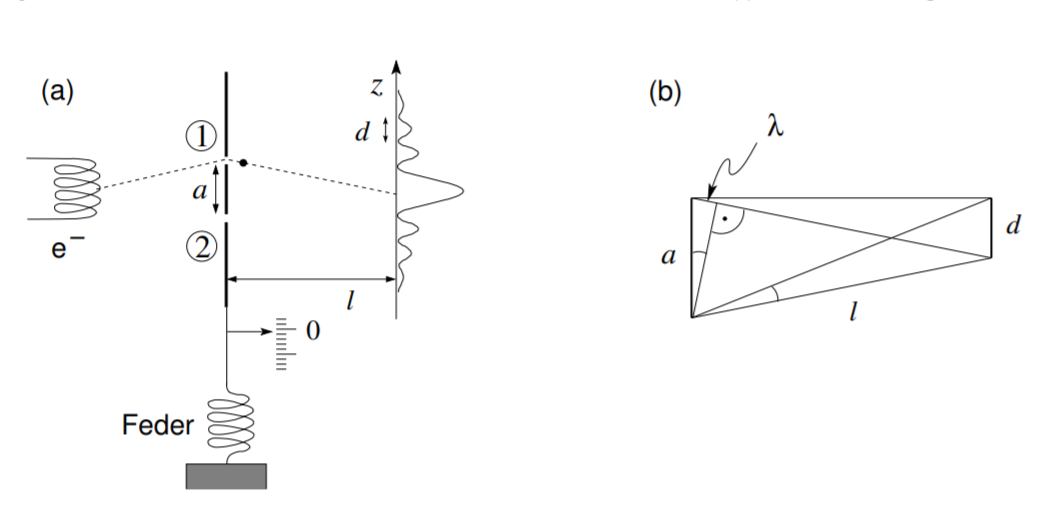
\includegraphics[scale=1]{1_5.PNG}
    \captionsetup{font={Large}}
    \caption{Double-slit experiment with detection: The deflection of the screen is intended to give indications of the passage of the small particle. This arrangement automatically leads to the Heisenberg uncertainty principle.}
    \label{fig:1.5}
\end{figure}
\\ \\
In summary, we note the following points:
\begin{itemize}
    \item[-] Propagation: Propagation always happens as a wave and involved the amplitude $\Phi$.
    \item[-] Detection: Detection always happens as particles and involved the probability $P = | \Phi |^2$.
    \item[-] Observation: Any observation fixes the propagation and destroys place the interference formation $\Phi = \sum_i \Phi_i$ in the total amplitude.
\end{itemize}

The consistency of QM demands even more astonishing effects: instead of the alternatives in the double-slit scattering experiment we consider the Figure 1.6 sketched particle-particle scattering with also two alternatives (here the so-called 'quantum alternatives' replace the simple paths).\\
Let $\Phi_{AB}(i, j)$ be the amplitude for the process (or quantum alternative) particle from A according to $i$, that of B according to $j$. From the symmetry of arrangement follows immediately: $\Phi_{AB}(1, 2) = \Phi_{AB}(2, 1)$. Are the particle types different in A and B, it is always possible to determine which type of particle in which detector arrived. There is no interference between the `paths' $A\to 1, B\to 2$ and $A\to 2, B\to 1$ and the coincidence measurement is by the probability
\begin{equation}
P_{\text {Koin }}=\left|\Phi_{\mathrm{AB}}(1,2)\right|^{2}+\left|\Phi_{\mathrm{AB}}(2,1)\right|^{2}=2 p
\end{equation}
%公式1.5
%图1.6
\begin{figure}[ht]
    \centering
    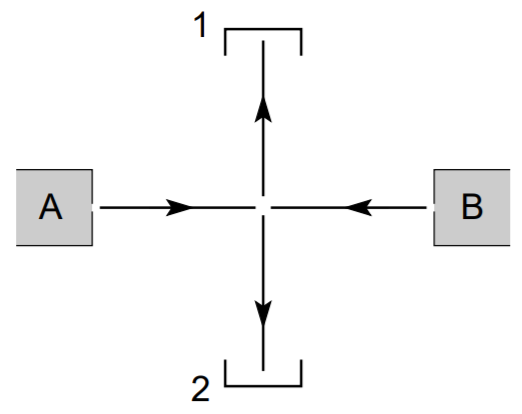
\includegraphics[scale=1]{1_6.PNG}
    \captionsetup{font={Large}}
    \caption{Particle Scattering: particles are emitted from sources A and B and measured in detectors 1 and 2.}
    \label{fig:1.6}
\end{figure}
%PAGE21
\\ \\
(PKoin gives the probability of having a particle in the same time to measure detector 1 and the second particle in Figure 2.) Are the particles identical,
about $^{4}He$, $\alpha$-particles, spin-0-bosons, so we can do the 'paths' do not differ and therefore get 
\\
\begin{equation}
P_{\mathrm{Koin}}=\left|\Phi_{\mathrm{AB}}(1,2)+\Phi_{\mathrm{AB}}(2,1)\right|^{2}=4 p
\end{equation}\\
%公式1.6
in accordance with the experiments. If you bring the experiment with your identical particles such as $^{3}He$ atoms, protons $p$, neutrons $n$, electrons $e^-$, or other so-called spin-1 = 2 fermions, so the paths are still indistinguishable (if the spins are aligned the same way), but we receive(if the spins are different, we get again $P_{Koin} = 2p$, since here is a criterion to distinguish the particles, the interference of both paths therefore
get lost.)
\\
\begin{equation}
P_{\mathrm{Koin}}=\left|\Phi_{\mathrm{AB}}(1,2)-\Phi_{\mathrm{AB}}(2,1)\right|^{2}=0
\end{equation}\\
%公式1.7
The result for bosons is in direct agreement with the conjecture
\\
$$
P_{\mathrm{Koin}}=\left|\sum_{\text {Pfade }} \Phi_{\mathrm{Pfad}} \mathrm{c}\right|^{2}
$$\\
%公式
we sum the amplitudes before squaring over paths C and generate thus an interference term. At Fermions you'll find exactly how bosons interfere with the same spins, however, the `swapped' paths $A\to 1, B\to 2$ and $A\to 2, B\to 1$ with different signs
into the sum,
\\
$$
P_{\mathrm{Koin}}=\left|\sum_{\text {Pfade }}(-1)^{v} \Phi_{\mathrm{Plad}} \mathrm{C}\right|^{2}
$$
$$
P_{\mathrm{Koin}}=\left|\sum_{\text {Pfade }}(-1)^{v} \Phi_{\mathrm{Plad}} \mathrm{C}\right|^{2}
$$\\
%公式
Another consistent input gives neutron scattering with polarized
%PAGE 22
%图1.7
\begin{figure}[ht]
    \centering
    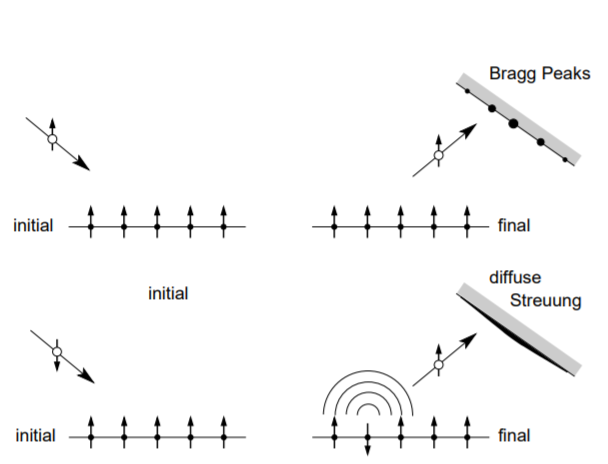
\includegraphics[scale=1]{1_7.PNG}
    \captionsetup{font={Large}}
    \caption{Scattering of neutrons on atoms with polarized spins. The interference is destroyed when the neutron releases a spin excitation that allows the scatter partner to identify itself.}
    \label{fig:1.7}
\end{figure}
neutrons on the polarized crystal, such as Figure 1.7: here two interference terms due to the summation over different scattering paths.
This interference is destroyed as soon as the information at which atom
neutron scattered was available. These experiments and ideas
lead us to a method for calculating the probabilities $P$
for a process: in order to find $P$ we have to use the possibly indistinguishable ones
determine and sum paths C and their amplitudes $\Phi_{PathC}$
according to (1.1).
For one-particle problems, $ v = 0$ and a path represents a path in the
physical space $\mathbb{R}^n$ represents; the probability for a process is
then through
\\
\begin{equation}
P=\left|\sum_{\text {Paths }} \Phi_{\text {Pfad }} C\right|^{2}
\end{equation}
%公式1.8
given. The two problems that need to be solved are:
\begin{itemize}
    \item What is the amplitude path $\Phi_{Pfad C}$ for any path $C$?
    \item Which means $\sum_{Paths}$?
\end{itemize}

\section{Path Integrals} 
There are usually not just two classical paths, but infinitely many paths,
see Figure 1.9.3(It puts a magnetic flux behind in an experiment with electrons the screen and between the paths (without the particles tracing a field)
this one additional phase diversity $(1/\Phi_0)\int Adl = \Phi/\Phi_0, \Phi_0=hc/e$ between the two paths which displace the interference pattern on the detector screen-- this is the famous Aharonov-Bohm Effect (1959), possibly discovered by Walter
Franz in Danzig (1939) and Werner Ehrenberg and Ray Siday (1949) in London, cf.
arXiv: 1304.4736v1.)
%PAGE 23
%图1.8 1.9
\begin{figure}[ht]
    \centering
    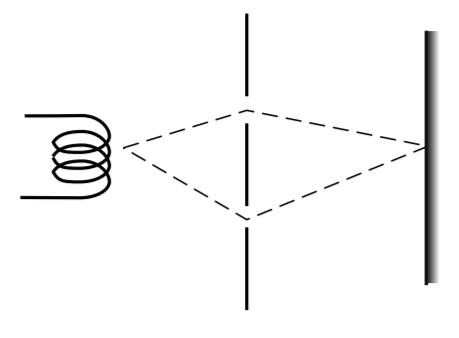
\includegraphics[scale=1]{1_8.PNG}
    \captionsetup{font={Large}}
    \caption{Two classic paths connect the source and
    the detector.}
    \label{fig:1.8}
\end{figure}
\begin{figure}[ht]
    \centering
    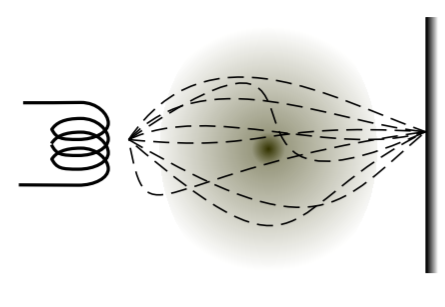
\includegraphics[scale=1]{1_9.PNG}
    \captionsetup{font={Large}}
    \caption{In quantum mechanics, all paths leading from the source to the detector contribute to the result.}
    \label{fig:1.9}
\end{figure}
\\ \\
A path is a function $y (x)$ or, in parametric form, a vector $(x (t), y (t))$ with the curve parameter $t$. Obviously, with $t$ mostly
meant the time. In general, a path is a vector-valued function $\vec{r} (t)$,
$\vec{r} \in \mathbb{R}^n$, where $\vec{r}$ indicates the position.

\subsection{Classical mechanics}
In classical mechanics, the movement of a particle realizes exactly one path $\vec{r} (t)$, namely, the one with the smallest effect. We consider the one-dimensional case. Let $L (x; \dot{x}; t)$ be the Lagrange function, $S=\int_{ta}^{tb}dtL(x,\dot{x}, t)$ the effect; their variation $\delta S = 0$ gives us the classical path $\bar{x}$ as a solution to an initial value problem. Explicit you are for the variation (use the functional derivative $\delta f (x)/\delta f(x') = \delta(x-x')$
in combination with the chain rule and a partial integration; here,
$f (x)\to x (t))$
\\
\begin{equation}
\begin{aligned} \frac{\delta \mathcal{S}\left[x\left(t^{\prime}\right)\right]}{\delta x(t)} &=\int_{t_{a}}^{t_{b}} d t^{\prime}\left[\frac{\partial \mathcal{L}}{\partial x} \frac{\delta x\left(t^{\prime}\right)}{\delta x(t)}+\frac{\partial \mathcal{L}}{\partial \dot{x}} \frac{\delta \dot{x}\left(t^{\prime}\right)}{\delta x(t)}\right] \\ &=\int_{t_{a}}^{t_{b}} d t^{\prime}\left[\frac{\partial \mathcal{L}}{\partial x} \delta\left(t-t^{\prime}\right)+\frac{\partial \mathcal{L}}{\partial \dot{x}} \dot{\delta}\left(t-t^{\prime}\right)\right] \\ &=\frac{\partial \mathcal{L}}{\partial x}+\left.\frac{\partial \mathcal{L}}{\partial \dot{x}} \delta\left(t-t^{\prime}\right)\right|_{t^{\prime}=t_{a}} ^{t_{b}}-\frac{d}{d t} \frac{\partial \mathcal{L}}{\partial \dot{x}}=0 \end{aligned}
\end{equation}\\
%公式1.9
%PAGE 24
\\
The boundary term is eliminated with the boundary conditions $\delta x (ta) =\delta x (tb) = 0$
and we get the Euler-Lagrange equation:
\\
\begin{equation}
\frac{d}{d t}\left(\frac{\partial \mathcal{L}}{\partial \dot{x}}\right)-\frac{\partial \mathcal{L}}{\partial x}=0
\end{equation}
\\
%公式1.10
The functional $S [x (t)]$ is then extreme for the path $\bar{x} (t)$. There are
different types of extremal points, cf. see Figure 1.10.
%图1.10
\begin{figure}[ht]
    \centering
    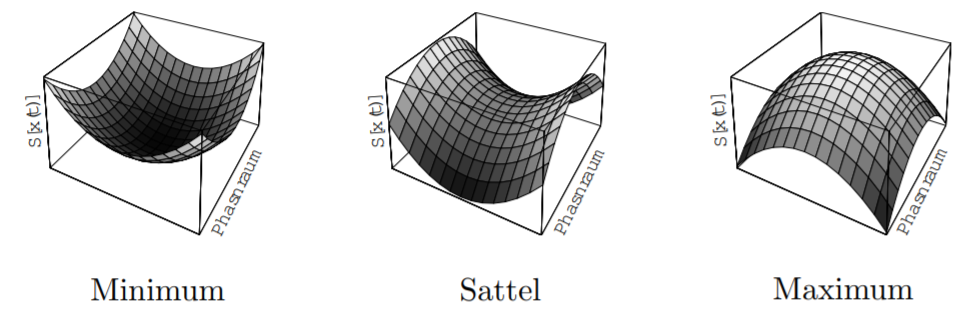
\includegraphics[scale=1]{1_10.PNG}
    \captionsetup{font={Large}}
    \caption{Different extremes of the effect $S[x(t)]$ in the phase space}
    \label{fig:1.10}
\end{figure}
\subsection{Quantum Mechanics}
According to Heisenberg's principle of blur, we can not fix $x (t)$. The blur is in effect and of the order of magnitude $h$, the effect quantum. From this one can assume that the relevant parameters is the dimensionless effect $S / h$. Next we search
a complex amplitude $\Phi[x (t)] \in C$ for the path $x (t)$. This amplitude describes the wave character of the particle, which is why we use a dimensionless
Need phase $\phi[x (t)]$. The approach $\phi[x (t)]/2\pi = S/h$ for the phase gives the amplitude
\\
\begin{equation}
\Phi[x(t)] \sim e^{i \mathcal{S}[x(t)] / \hbar}
\end{equation}\\
%公式1.11
for the path $x (t)$. Note that this is not a derivation of quantum mechanics
is. The following correspondences result(In addition, from later versions or the textbooks of Messiah,
p. 222, as well as Fetter, Walecka, p. 184, see also the Hamilton-Jakobi formalism in the
Mechanics or the quasi-classical approximation in Chap. 10)
\\
\begin{equation}
\begin{array}{c}{\text { quantum mechanics } \cong \text { wave optics }} \\ 
{\qquad \begin{aligned} 
\hbar\to 0 \downarrow \text { Approximation } & \text { Eikonalapprox } \downarrow \lambda \rightarrow 0 \\ \text { classical mechanics } & \cong \text { geometric appearance } \end{aligned}}\end{array}
\end{equation}\\
%公式1.12
%PAGE 25
\\
The combination of (1.8) and (1.11) gives the amplitude $K (b, a)$
which describes the propagation of a particle from $a$ to $b$
\\\begin{equation}
K(b, a)=\sum_{x(t)} \Phi[x(t)]
\end{equation}\\
%公式1.13
and for the (relative) probability $P (b, a)$ that the particle is undisturbed
from $a$ to $b$ (ie without destroying the interference)\\
\begin{equation}
P(b, a)=|K(b, a)|^{2}
\end{equation}\\
%公式1.14
$K (b, a)$ is called the \textbf{propagator} and describes the 'movement' of the particle of
$a$ to $b$.
%图1.11
\begin{figure}[ht]
    \centering
    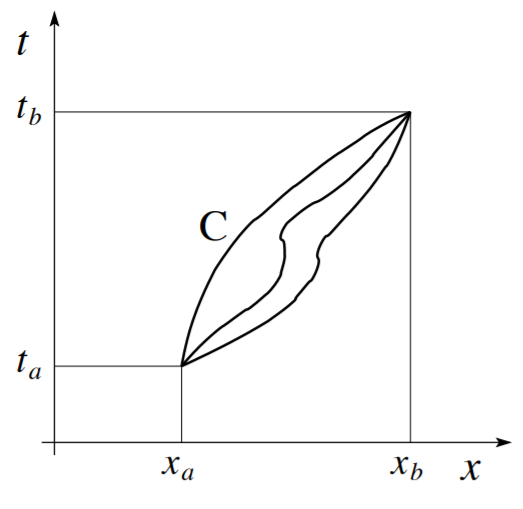
\includegraphics[scale=1]{1_11.PNG}
    \captionsetup{font={Large}}
    \caption{In the path integral is summed over all paths $C$ beginning in $a = (xa, ta)$ and ending in $b = (xb, tb)$.}
    \label{fig:1.11}
\end{figure}
\\\textbf{Classic Limes}\\\\
Consider (1.13). Now suppose that the typical effect $S [x (t)]$
for $x (t)$ from $a$ to $b$ of the order of magnitude S0 let. $S_0 / h$ then gives the
Phase rotation in amplitude to the path from $a$ to $b$. If $S_0$ big
is, generic adjacent paths $x (t)$ and $x (t) + \delta x (t)$
already many revolutions, that is, they are strongly out of phase and
therefore interfere destructively; their sum is small. Only special paths with
Deviations $\delta S_0/h \ll 1$ contribute to $K (b, a)$; such paths are close by
of the classical path where $\delta S [\bar{x} (t)] = 0$, that is, the relevant trajectory
the classical, $\bar{x} (t)$. For big $S_0$ (big masses, big energies, ...)
only the very nearest environment of the classical path $\bar{x} (t)$ to the integral and we discover the results of classical physics; also goes for $h\to 0$ quantum mechanics into classical mechanics.
%PAGE 26
Semi-classical approximation: in the semi-classical approximation
let's write the propagator as a product of a volume factor and
a phase factor, the latter via the effect over the classical
Path is evaluated,
\\
\begin{equation}
K(b, a)=V(b) e^{i \mathcal{S}[\bar{x}] / \hbar}
\end{equation}\\
%公式 1.15
The volume factor $V (b)$ is a smooth function; the strong variation with the
Change of the end point b is in the phase factor $e^{iS[\bar x]/\bar{h}}$. The name
'half-classic' refers to the description of the particle (system) via
a wave function whose phase is determined by the classical effect
is. $V (b)$ indicates the volume of the paths which contribute to $K$,
see. Figure 1.12.
%图 1.12
\begin{figure}[ht]
    \centering
    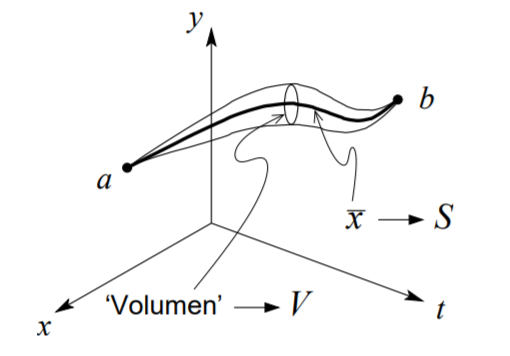
\includegraphics[scale=1]{1_12.PNG}
    \captionsetup{font={Large}}
    \caption{In the semi-classical approximation, the propagator $K (b, a)$ results as a product of a volume factor $V (b)$ and a phase factor $exp [iS [\bar{x}]/\hbar]$ with an effect $S$ evaluated over the classical path $\bar{x}(t)$.}
    \label{fig:1.12}
\end{figure}
\\
\textbf{Summation over paths}\\\\
The Riemann integral over a function $f (x)$ is defined as a limit the Riemann sum
\\
\begin{equation}
\lim _{\eta \rightarrow 0}\left[\eta \sum_{i} f\left(x_{i}\right)\right]
\end{equation}\\
%公式 1.16
where the measure is given by the 'breadth' of an interval, cf. Illustration
1.13. Similarly, we de nieren a sum of paths by
Discretize time and space, and take the appropriate limit, cf.
Figure 1.13. For each time step $t_i$, we sum over all possible positions $x_i$,
\\
\begin{equation}
K(b, a)=\lim _{\varepsilon \rightarrow 0} \frac{1}{A} \int_{-\infty}^{\infty} \frac{d x_{1}}{A} \int_{-\infty}^{\infty} \frac{d x_{2}}{A} \cdots \int_{-\infty}^{\infty} \frac{d x_{N-1}}{A} e^{i \mathcal{S}[x(t)] / \hbar}
\end{equation}\\
%公式 1.17
It raises the question of the value of Mass A. As this constant
is universal (analogous to the Riemann integral), it satisfies the path integral
%PAGE27
%Figure 1.13
\begin{figure}[ht]
    \centering
    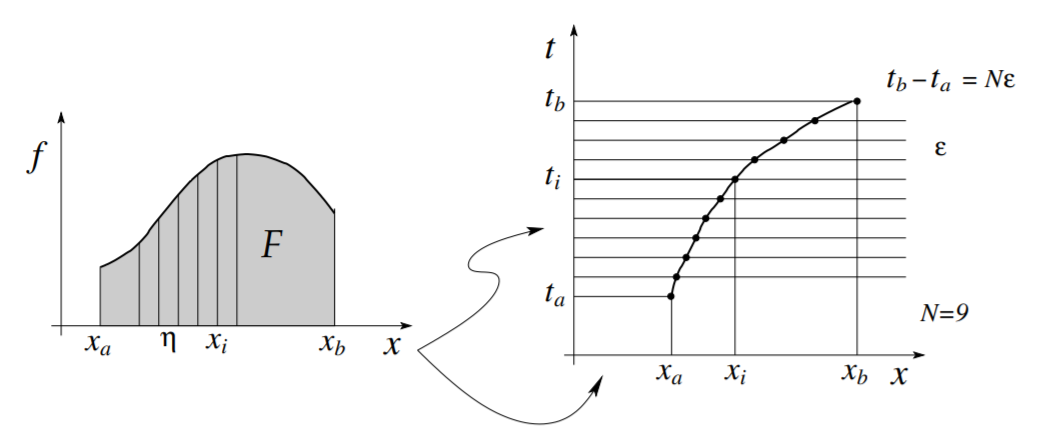
\includegraphics[scale=1]{1_13.PNG}
    \captionsetup{font={Large}}
    \caption{Left: Riemann integral with support points $x_i$ in the distance. Right: In the path integral is summed over all paths that connect $a = (xa, ta)$ to $b = (xb, tb)$. In this case, both the $x$-axis and the time $t$ are discretized, with intervals $dx$ (as in the Riemann integral) in place and $\epsilon$ in the time interval. $\epsilon$ defines the measure $A=\sqrt{2\pi i\hbar\epsilon/m}$}
    \label{fig:1.13}
\end{figure}
for a simple case. We consider a free particle,
\\
$$
\mathcal{L}(x, \dot{x}, t)=\mathcal{L}(\dot{x})=\frac{m}{2} \dot{x}^{2} \approx \frac{m}{2}\left(\frac{x_{i+1}-x_{i}}{\varepsilon}\right)^{2}
$$\\
%公式
and generally, $\mathcal{L}[(x_{i + 1} + x_i) = 2, (x_{i + 1}- x_i) /\epsilon, (t_{i + 1} + t_i) / 2]$. In the discretized
Form we can calculate the occurring integrals,
\\
$$
\begin{aligned} 
K(b, a)= & \lim _{\varepsilon \rightarrow 0} A^{-N}\left[\prod_{i=1}^{N-1} \int d x_{i}\right] e^{\frac{i m}{2 \hbar} \varepsilon \sum_{j=0}^{N-1}\left(\frac{x_{j+1}-x_{j}}{\varepsilon}\right)^{2}} 
\\
= & \lim _{\varepsilon \rightarrow 0} A^{-N}\left[\prod_{i=2}^{N-1} \int d x_{i}\right] 
\begin{array}
    {l}{\frac{i m}{2 \hbar \varepsilon} \sum_{j=2}^{N-1}\left(x_{j+1}-x_{j}\right)^{2}}
\end{array} 
\\ 
%\qquad \begin{aligned}
= & 2\left[x_{1}-\left(x_{2}+x_{a}\right) / 2\right]^{2}+x_{2}^{2}+x_{a}^{2}-\left(x_{2}+x_{a}\right)^{2} / 2 
\\
= & 2\left[x_{1}-\left(x_{2}+x_{a}\right) / 2\right]^{2}+\left(x_{2}-x_{a}\right)^{2} / 2 
\\ \rightarrow & \sqrt{\frac{\pi i \hbar 2 \varepsilon}{2 m}} e^{\frac{i m}{2 h(2 \varepsilon)}\left(x_{2}-x_{a}\right)^{2}} %\end{aligned} 
\end{aligned}
$$\\
$$
\downarrow \text { mit Gauss: } \int d x e^{i a x^{2}}=\sqrt{\frac{i \pi}{a}} \text { und } \int d x e^{-\frac{x^{2}}{2 \sigma}}=\sqrt{2 \pi \sigma}
$$
$$\\
\begin{aligned}=\lim _{\varepsilon \rightarrow 0} A^{-N}\left(\frac{2 \pi i \hbar \varepsilon}{2 m}\right)^{1 / 2} &\left[\prod_{i=3}^{N-1} \int d x_{i}\right] e^{\frac{i m}{2 \hbar \varepsilon} \sum_{j=3}^{N-1}\left(x_{j+1}-x_{j}\right)^{2}} \\ & \times \underbrace{\int d x_{2} e^{\frac{i m}{2 \hbar \varepsilon}\left[\left(x_{3}-x_{2}\right)^{2}+\frac{1}{2}\left(x_{2}-x_{a}\right)^{2}\right]}}_{\sqrt{\frac{2 \pi i \hbar 2 \varepsilon}{3 m}} e^{\frac{i m}{2 \hbar(3 \varepsilon)}}\left(x_{3}-x_{a}\right)^{2}} \end{aligned}
$$\\
$$
\begin{aligned} &=\lim _{\varepsilon \rightarrow 0} A^{-N}\left(\frac{2 \pi i \hbar \varepsilon}{m}\right)^{(N-1) / 2} \frac{1}{\sqrt{2}} \cdot \sqrt{\frac{2}{3}} \cdot \sqrt{\frac{3}{4}} \cdots \\ &=\lim _{\varepsilon \rightarrow 0} \frac{1}{A}\left(\frac{2 \pi i \hbar \varepsilon}{A^{2} m}\right)^{(N-1) / 2} \sqrt{\frac{\varepsilon}{\varepsilon N}} e^{\frac{i m}{2 \hbar\left(t_{b}-t_{a}\right)}\left(x_{b}-x_{a}\right)^{2}} \end{aligned}
$$\\
\begin{equation}
\begin{array}{l}{\downarrow \Rightarrow A=\sqrt{\frac{2 \pi i \hbar \varepsilon}{m}}} \\ {=\sqrt{\frac{m}{2 \pi i \hbar\left(t_{b}-t_{a}\right)}} \exp \left[\frac{i m\left(x_{b}-x_{a}\right)^{2}}{2 \hbar\left(t_{b}-t_{a}\right)}\right]}\end{array}
\end{equation}\\
%公式
With the simplified start and end coordinates $t_a = 0, t_b = t, x_a = 0$
and $x_b = x$ we ​​find the simpler form for K
\\
\begin{equation}
K(x, t)=\sqrt{\frac{m}{2 \pi i \hbar t}} \exp \left[\frac{i m x^{2}}{2 \hbar t}\right]
\end{equation}\\
%公式 1.19
Definition: under the path integral
\begin{equation}
K(b, a) \equiv \int_{a}^{b} \mathcal{D}[x(t)] e^{i S[x(t)] / \hbar}
\end{equation}
%公式 1.20
one understands the expression
\\
\begin{equation}
\begin{aligned} K(b, a) &=\lim _{\varepsilon \rightarrow 0}\left(\frac{m}{2 \pi i \hbar \varepsilon}\right)^{N / 2} \int_{-\infty}^{\infty} \prod_{i=1}^{N-1} d x_{i} \\ & \times \exp \left[\frac{i \varepsilon}{\hbar} \sum_{j=0}^{N-1} \mathcal{L}\left(\frac{x_{j+1}+x_{j}}{2}, \frac{x_{j+1}-x_{j}}{\varepsilon}, \frac{t_{j+1}+t_{j}}{2}\right)\right] \end{aligned}
\end{equation}\\
%公式 1.21
where $N = (t_b - t_a) /\epsilon, (x_0, t_0) = a$ and $(x_N, t_N) = b$.
%PAGE 29
An illustration of the propagator $K (x, t)$ of the free particle (1.19) is in the
Figures 1.14 and 1.15 given; These suggest the de nition of one
local wavelength $\lambda$ and a local period $T$. The local wavelength is $\lambda$
%Figure  1.14
\begin{figure}[ht]
    \centering
    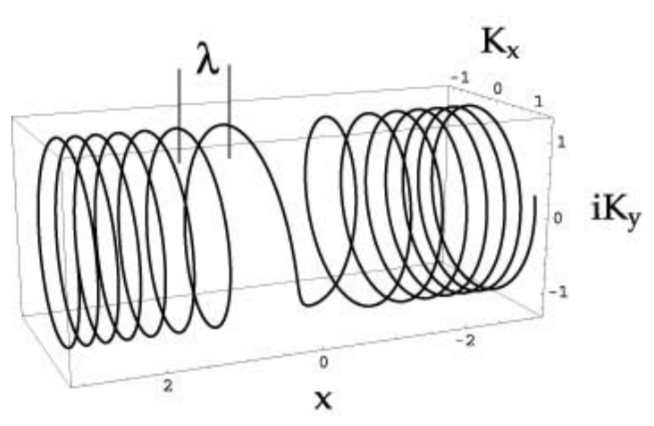
\includegraphics[scale=1]{1_14.PNG}
    \captionsetup{font={Large}}
    \caption{$K (x, t)$ for the free particle as a function of $x$ at fixed $t$ leads to the definition of a local wave with increasing
    distance $x$ decreases.}
    \label{fig:1.14}
\end{figure}
, see Figure 1.14 can be found in the approximation of large distances $x\gg \lambda$
calculate as
\\
\begin{equation}
\begin{aligned} m \frac{(x+\lambda)^{2}-x^{2}}{2 \hbar t} &=\frac{m x \lambda}{\hbar t}\left(1+\frac{\lambda}{2 x}\right)=2 \pi \\ \lambda & \stackrel{x \gg \lambda}{=} \frac{h}{m v}=h / p \end{aligned}
\end{equation}\\
%公式 1.22
$\Rightarrow$ Particles which contribute to $K$ in $x$ at time $t$ have the
Impuls $p = mx / t$ and are quantum mechanically as a wave with $\lambda = h/p$
described.
The local period T (Figure 1.15) may be longer in the approximation
Times $t\gg T$ determine
\\
\begin{equation}
\frac{m x^{2}}{2 \hbar}\left(\frac{1}{t}-\frac{1}{t+T}\right)=\frac{m x^{2}}{2 \hbar t^{2}}\left(\frac{T}{1+T / t}\right)=2 \pi
\end{equation}\\
%公式 1.23
Particles that contribute to $K$ in $x$ at time $t$ have the energy $E = m (x / t)^2 / 2$ and are quantum mechanically as wave with period $T = h / E$ described. The angular frequency of the wave is given by
\\
\begin{equation}
\omega=\frac{2 \pi}{T} \stackrel{t \gg T}{=} \frac{1}{\hbar} \frac{m}{2}\left(\frac{x}{t}\right)^{2}=\frac{E}{\hbar}
\end{equation}\\
%公式 1.24
%PAGE 30
%Figure  1.15
\begin{figure}[ht]
    \centering
    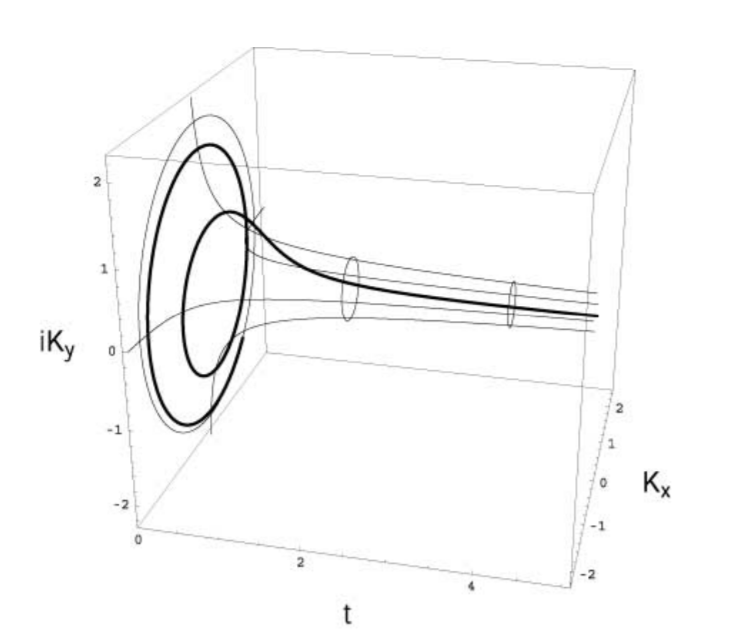
\includegraphics[scale=1]{1_15.PNG}
    \captionsetup{font={Large}}
    \caption{$K (x, t)$ for the free particle as a function of $t$ at fixed $x$, allows the definition of a local period $T$ which increases with increasing time.}
    \label{fig:1.15}
\end{figure}
\\
In general, we can have any propagator K in the semi-classical
Approximation $K (b, a) \sim exp [iS_{kl}(b, a)/\hbar]$ by a local wave and
describe a local period: the dominant dependency of $K (b)$
appears in the phase factor and allows the definition of the local wave
and the local period according to
\\
\begin{equation}
\begin{array}{l}{h=2 \pi \hbar=S_{k l}\left(x_{b}+\lambda\right)-S_{k l}\left(x_{b}\right)=\lambda \frac{\partial S_{k l}}{\partial x_{b}}=\lambda p} \\ {h=2 \pi \hbar=S_{k l}\left(t_{b}+T\right)-S_{k l}\left(t_{b}\right)=T \frac{\partial S_{k l}}{\partial t_{b}}=T E}\end{array}
\end{equation}\\
%公式 1.25
\subsection{Product rule}
The propagator $K (b, a)$ is derived from partial propagations over subintervals
$(a, c)$ and $(c, b)$ are composed, whereby over all positions of the
Intermediate point $c$ is to sum, cf. Figure  1.16. The Additivit of the
Effect in the exponent leads to the product of the partial propagators; the
Factorization in subpaths can be repeated iteratively,
\\
\begin{equation}
\begin{split}
K(b,a)&
=\int \mathcal{D}[x(t)] e^{(i / \hbar)[S(b, c)+S(c, a)]} \\
&=\int d x_{c} K(b, c) K(c, a) \\ 
&=\int \prod_{i=1}^{N-1} d x_{i} K\left(b, x_{N-1}\right) K\left(x_{N-1}, x_{N-2}\right) \cdots K\left(x_{1}, x_{a}\right)
\end{split}
\end{equation}\\
%公式 1.26

%PAGE 31
%Figure  1.16
\begin{figure}[ht]
    \centering
    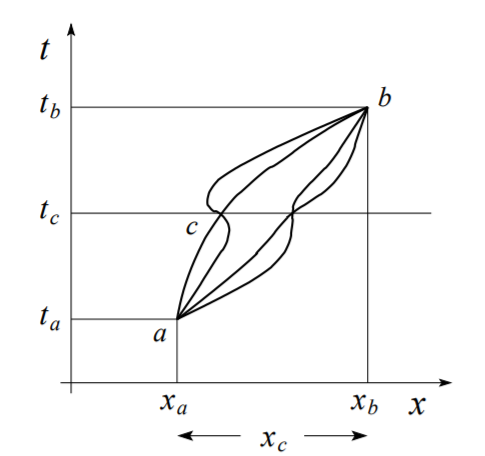
\includegraphics[scale=1]{1_16.PNG}
    \captionsetup{font={Large}}
    \caption{Illustration of the product rule with an intermediate step at $t_c$.}
    \label{fig:1.16}
\end{figure}
\subsection{Wave function}
$K (b, a)$ describes the propagation of a particle from $a$ to $b$. We generalize
this result by looking at a particle of which
we do not have its initial position (at a) but only the amplitude $\Psi(a) = \Psi(x_a, t_a)$ know. Then according to (1.26) the following amplitude results in $b$,
\begin{equation}
\Psi\left(x_{b}, t_{b}\right)=\int_{-\infty}^{\infty} d x_{a} K\left(x_{b}, t_{b} ; x_{a}, t_{a}\right) \Psi\left(x_{a}, t_{a}\right)
\end{equation}
%公式 1.27
the wave function of the particle at a later time $t_b$. $|\Psi (x_b, t_b)|^2$
is the (relative) probability of finding the particle in $x_b$ at time $t_b$.
Note: The knowledge of $\Psi$ at one time (here $t_a$) determines $\Psi$ for all times.
This results in a differential equation of the first order for the time evolution
in $d / dt$.
In classical mechanics two initial conditions $x$ and $\partial_t x$ are required,
to set the particle trajectory. That is why in the classic
Mechanics a di erential equation 2nd order in $d / dt$ from ot.

%PAGE 32
\section{Generalizations}
We consider three generalizations for the propagator $K$, the particle
in the potential $V (x)$, the particle in the multidimensional space $\mathbb{R}^n$, and
the propagator for several particles.

\subsection{Particles in the potential $V (x)$}
We can exactly determine the propagator $K$ if and only if the Lagrange function
$\mathcal{L} (x, \dot{x}, t)$ is a 2nd order polynomial in $x$ and $\dot{x}$. The reason
This restriction is that we only calculate Gauss integrals
k may. It was
\\
\begin{equation}
\mathcal{L}=a \dot{x}^{2}+b \dot{x} x+c x^{2}+d \dot{x}+e x+f
\end{equation}\\
%公式 1.28
wanted is $K$,
\\
\begin{equation}
K(b, a)=\int_{a}^{b} \mathcal{D}[x(t)] \exp \left[\frac{i}{\hbar} \int_{t_{a}}^{t_{b}} d t \mathcal{L}(x, \dot{x}, t)\right]
\end{equation}\\
%公式 1.29
Moody way: as before on page 28. Easier: Let $\delta S(\bar{x}) = 0$, with the
classical path $\bar{x}$. Then with $x = \bar{x} + y$,
\\
\begin{equation}
S[x(t)]=S[\bar{x}(t)]+\int_{t_{a}}^{t_{b}} d t\left[a \dot{y}^{2}+b \dot{y} y+c y^{2}\right]
\end{equation}\\
%公式 01.30
the contributions of the terms linear in $y$ and $\dot{y}$ vanish because $\delta S (\bar{x}) = 0$. Thus
we will
\\
\begin{equation}
\begin{aligned} K(b, a) &=\exp \left[\frac{i}{\hbar} S[\bar{x}(t)]\right] \int_{0}^{0} \mathcal{D}[y(t)] \exp \left[\frac{i}{\hbar} \int_{t_{a}}^{t_{b}} d t\left[a \dot{y}^{2}+b \dot{y} y+c y^{2}\right]\right] \\ &=\exp \left[\frac{i}{\hbar} S[\bar{x}(t)]\right] F\left(t_{b}, t_{a}\right) \end{aligned}
\end{equation}\\
%公式 1.31
a development around the classical way. The whole dependency of
the positions $x_a, x_b$ appears in the exponential factor via the classic
Path $\bar{x}(t)$.
Now let $\mathcal{L} = T - V$, as known from classical mechanics. Then
we write again
\\
\begin{equation}
\begin{aligned} V(x) &=V(\bar{x}+y)=V(\bar{x})+y V^{\prime}(\bar{x})+\frac{y^{2}}{2} V^{\prime \prime}(\bar{x})+\frac{y^{3}}{6} V^{\prime \prime \prime}(\bar{x})+\cdots \\ & \downarrow \text { quadratische Approximation } \\ & \cong V(\bar{x})+y V^{\prime}(\bar{x})+\frac{y^{2}}{2} V^{\prime \prime}(\bar{x}) \end{aligned}
\end{equation}\\
%公式 1:32
%PAGE 33
That's how we get
\\
\begin{equation}
\begin{aligned} K(b, a) & \cong \exp [i S[\bar{x}(t)] / \hbar] \\ & \times \int_{0}^{0} \mathcal{D}[y(t)] \exp \left[\frac{i}{\hbar} \int_{t_{a}}^{t_{b}} d t\left(\frac{m}{2} \dot{y}^{2}-\frac{m \omega^{2}}{2} y^{2}\right)\right] \end{aligned}
\end{equation}\\
%公式 1:33
with $w^2 = V^{''}(\bar{x}(t))/m$ analogous to the harmonic oscillator. This approximation
is good if one of the following points is true:
\{$S/\hbar \gg 1$, then y is small and $y^3$ is negligible.
\{$V$ square, so (1.33) is exact.
\{$V$ smooth, so $V^{(n)}$ for $n\geq 3$ is small$\to$ WKB (Wenzel-Kramers Brillouin).
\{$tb - ta$ small and thus $y$ is small because otherwise $T$ is big.
1.3.2 Particles in marg
The definition (1.20) of the path integral for $n = 1$ is immediately apparent
Generalize movements in high dimensional spaces,
\\
\begin{equation}
\begin{aligned} K(\vec{b}, \vec{a})=& \int_{\vec{a}}^{\vec{b}} \mathcal{D}[\vec{r}(t)] \exp (i S[\vec{r}(t)] / \hbar) \\ & \quad \operatorname{mit} \mathcal{D}[\vec{r}(t)]=\mathcal{D}\left[x_{1}(t)\right] \cdots \mathcal{D}\left[x_{n}(t)\right] \end{aligned}
\end{equation}\\
%公式 1:34
that is, the path integral involves a factor for each dimension. Note
that the problem is generally not factored; the movements in the
different directions are not independent.
1.3.3 Several particles
Again, the generalization is immediately obvious: again occurs
a product of path integrals, similar to 1.3.2. For $k$ particles that
propagate from $\vec{ak}$ to $\vec{bk}$, let the propagator write as
\\
\begin{equation}
\begin{aligned} K\left(\vec{b}_{1}, \cdots, \vec{b}_{k} ; \vec{a}_{1}, \ldots, \vec{a}_{k}\right)=& \int_{\vec{a}_{1}}^{\vec{b}_{1}} \mathcal{D}\left[\vec{r}_{1}(t)\right] \cdots \int_{\vec{a}_{k}}^{\vec{b}_{k}} \mathcal{D}\left[\vec{r}_{k}(t)\right] \\ & \times \exp \left[\frac{i}{\hbar} S\left[\vec{r}_{1}(t), \ldots, \vec{r}_{k}(t)\right]\right] \end{aligned}
\end{equation}\\
%公式 1:35
%PAGE 34
For two interacting particles in the $\mathbb{R}^1\times \mathbb{R}^1$ with the Lagrangian
\\
\begin{equation}
\mathcal{L}=\frac{m}{2} \dot{x}^{2}+\frac{M}{2} \dot{X}^{2}-V(x, X, t)
\end{equation}\\
%公式 1:36
If you find the propagator,
\\
\begin{equation}
\begin{array}{c}{K\left(x_{b}, X_{b}, t_{b} ; x_{a}, X_{a}, t_{a}\right)=\int \mathcal{D}[x(t)] \mathcal{D}[X(t)] \exp \left[\frac{i}{\hbar} S[x(t), X(t)]\right]} \\ {=\int \mathcal{D}[x(t)] \exp \left[\frac{i}{\hbar} \int_{t_{a}}^{t_{b}} \frac{m}{2} \dot{x}^{2} d t\right] T[x(t)]}\end{array}
\end{equation}\\
%公式 1:37
with the functional $T [x (t)]$ given as a path integral over the coordinate
$X (t)$ of the other particle (the In
uenzintegral)
\\
\begin{equation}
T[x(t)]=\int \mathcal{D}[X(t)] \exp \left[\frac{i}{\hbar} \int_{t_{a}}^{t_{b}}\left[M \dot{X}^{2} / 2-V(x, X, t)\right]\right]
\end{equation}\\
%公式 1:38
If $V = V_x (x) + V_X(X)$, so no interaction takes place, then
separates the system and
\\
\begin{equation}
K\left(x_{b}, X_{b}, t_{b} ; x_{a}, X_{a}, t_{a}\right)=K_{x}\left(x_{b}, t_{b} ; x_{a}, t_{a}\right) \times K_{X}\left(X_{b}, t_{b} ; X_{a}, t_{a}\right)
\end{equation}\\
%公式 1:39
Dissipative Problems: In classical mechanics, a particle can be found
describe with friction by the dissipative dynamics $m\ddot{x}+\eta\dot{x}=-\partial_xV(x)$
the term $\eta\dot{x}$ describes the friction and implies that energy
is dissipated. The quantum mechanical description of this problem is
difficult because we have to resort to a Hamiltonian formulation.
Feynman and Vernon and later Caldeira and Leggett have suggested
to couple the system to a reservoir of harmonic oscillators
and then to integrate over the coordinates of the oscillators, cf.
Figure  1.17. The total system particles \& reservoir is by the Lagarian
%Figure  1.17
\begin{figure}[ht]
    \centering
    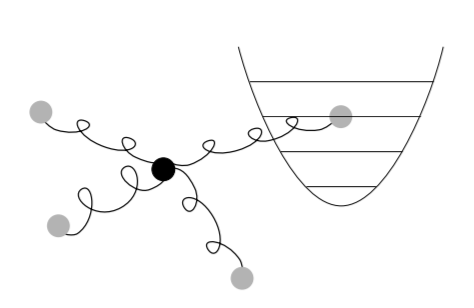
\includegraphics[scale=1]{1_17.PNG}
    \captionsetup{font={Large}}
    \caption{Description of a dissipative system: the coordinate is coupled to a reservoir of harmonic oscillators, which is then integrated.}
    \label{fig:1.17}
\end{figure}

%PAGE 35
%\\
\begin{equation}
\begin{array}{r}{\mathcal{L}=\frac{m}{2} \dot{x}^{2}-V(x)+\sum_{k}\left(\frac{M_{k}}{2} \dot{X}_{k}^{2}-\frac{M_{k} \omega_{k}^{2}}{2} X_{k}^{2}\right)} \\ {-\underbrace{\sum_{k} q_{k} x X_{k}}_{\text {lin. Koplung }}-\underbrace{\sum_{k} \frac{q_{k}^{2} x^{2}}{2 M_{k} \omega_{k}}}_{\text {Gegenterm }}}\end{array}
\end{equation}\\
%公式 1:40
described. The interaction is via the linear coupling term
$xX_k$ takes place; the counter-guarantor guarantees that the potential $V (x)$ through the bath
is not renormalized. After integration over the reservoir degrees of freedom
$X_k$ is the e ff effective propagator
\\
\begin{equation}
\begin{aligned} K\left(x_{b}, t_{b} ; x_{a}, t_{a}\right) &=\int \mathcal{D}[x(t)] \exp \left[\frac{i}{\hbar} S_{\mathrm{eff}}[x(t)]\right] \\ S_{\mathrm{eff}} &=\int d t\left[\frac{m}{2} \dot{x}^{2}-V(x)+\text { Dissipativer Term }\right] \end{aligned}
\end{equation}\\
%公式 1:41
Further details can be found in R.P. Feynman and F.L. Vernon, Annals of
Physics 24, 118 (1963) and in A.O. Caldeira and A.J. Leggett, Annals of
Physics 149, 374 (1983). (The work of Feynman and Vernon deals with the problem of real-time dynamics,
while Caldeira and Leggett are experiencing quantum statistical problems in the imaginary artefact
Discuss formalism.)

\section{Schrodinger equation}
We start from the relation (1.27), which is the evolution of the wave function
of a particle describes
\\
\begin{equation}
\Psi\left(x_{b}, t_{b}\right)=\int_{-\infty}^{\infty} d x_{a} K\left(x_{b}, t_{b} ; x_{a}, t_{a}\right) \Psi\left(x_{a}, t_{a}\right)
\end{equation}\\
%公式 1:42
it describes the dynamics of the system in an integral way. We
seek a di erential form of dynamics. Since (1.42) holds for all $t_b> t_a$,
we can choose $t = t_a$ and $t_b = t + \epsilon$ and with $\mathcal{L}=(m/2)\dot{x}^2-V(x,t)$
we receive
\\
\begin{equation}
\begin{aligned} \Psi(x, t+\varepsilon) &=\int \frac{d y}{A} \exp \left[\frac{i}{\hbar} \varepsilon \mathcal{L}\left(\frac{x+y}{2}, \frac{x-y}{\varepsilon}, t+\frac{\varepsilon}{2}\right)\right] \Psi(y, t) \\ &=\int \frac{d y}{A} \exp \left[\frac{i m}{2 \hbar \varepsilon}(x-y)^{2}\right] \exp \left[-\frac{i \varepsilon}{\hbar} V\left(\frac{x+y}{2}, t+\frac{\varepsilon}{2}\right)\right] \Psi(y, t) \end{aligned}
\end{equation}\\
%公式 1:43
%PAGE 36
It must be $x-y$ small, otherwise $T = m\dot{x}^2/2$ large. We de fi ne $y = x +\eta$,
with small, and $\eta$
\\
\begin{equation}
\Psi(x, t+\varepsilon)=\int \frac{d \eta}{A} \exp \left[\frac{i m \eta^{2}}{2 \hbar \varepsilon}\right] \exp \left[-\frac{i \varepsilon}{\hbar} V(x+\eta / 2, t+\varepsilon / 2)\right] \Psi(x+\eta, t)
\end{equation}\\
%公式 1:44
For $m\eta^2/2\hbar\epsilon>1$ the first factor oscillates strongly and thus cuts the
$\eta$-Integration ectively at
$\eta \sim \sqrt{\epsilon \hbar/m}$, we get a consistent one $\epsilon$ Development alright "if we develop to potencies $\epsilon$ and $\eta^2$,
\\\begin{equation}
\begin{aligned} \Psi(x, t)+\varepsilon \partial_{t} \Psi(x, t) \cong \int_{-\infty}^{\infty} \frac{d \eta}{A} \exp \left(\frac{i m \eta^{2}}{2 \hbar \varepsilon}\right)\left[1-\frac{i \varepsilon}{\hbar} V(x, t)\right] \\ \times\left[\Psi(x, t)+\eta \partial_{x} \Psi(x, t)+\frac{\eta^{2}}{2} \partial_{x}^{2} \Psi(x, t)\right] \end{aligned}
\end{equation}
\\
%公式 1:45
The evolution into orders of $\epsilon$ yields
$\epsilon^0$ terms:
\\
\begin{equation}
\begin{aligned} \Psi(x, t) &=\int_{-\infty}^{\infty} \frac{d \eta}{A} \exp \left(\frac{i m \eta^{2}}{2 \hbar \varepsilon}\right) \Psi(x, t) \\ &=\sqrt{\frac{2 \pi i \hbar \varepsilon}{m}} \frac{1}{A} \Psi(x, t) \\ \Rightarrow A &=\sqrt{\frac{2 \pi i \hbar \varepsilon}{m}} \end{aligned}
\end{equation}\\
%公式 1:46
This is the easiest way to find A.\\
$\epsilon^{1/2}$ terms:
\\
\begin{equation}
0=0 \quad\left(\int_{-\infty}^{\infty} d \eta \eta \exp \left[\frac{i m \eta^{2}}{2 \hbar \varepsilon}\right]=0\right)
\end{equation}\\
$\epsilon^1$ terms:
\\
\begin{equation}
\varepsilon \partial_{t} \Psi(x, t)=\underbrace{\int_{-\infty}^{\infty} \frac{d \eta}{2 A} \eta^{2} \exp \left[\frac{i m \eta^{2}}{2 \hbar \varepsilon}\right]}_{i \hbar \varepsilon / 2 m} \partial_{x}^{2} \Psi+\frac{\varepsilon}{i \hbar} V(x, t) \Psi(x, t)
\end{equation}\\
%公式 1:48
This gives us the Schrodinger equation
\\
\begin{equation}
i \hbar \partial_{t} \Psi=-\frac{\hbar^{2}}{2 m} \partial_{x}^{2} \Psi+V(x, t) \Psi
\end{equation}\\
%公式 1:49
%PAGE 37
\\\textbf{Remarks}\\
1. The Schrodinger equation (1.49) is a 1-th order differential equation, thus satisfies $\Psi(xm t = t_0)$ as an initial condition.\\
2. The time derivative $i\hbar \partial_t$ defines a Hamiltonian dynamics, which of the dissipative dynamics $\partial_t \Psi=D\partial^2_x\Psi$ is the Diffusion different (A typical example of the equation of the equation is that for the temperature T, that is, $\Psi(x, t) = T (x, t)$.\\
3. $K (x_2, t_2; x_1, t_1) = K (2; 1)$ is a solution of the Schr odinger equation
(1.49) for $t_2> t_1$:
\\
\begin{equation}
i \hbar \partial_{t_{2}} K(2,1)=-\frac{\hbar^{2}}{2 m} \partial_{x_{2}}^{2} K(2,1)+V(2) K(2,1)
\end{equation}\\
%公式 1:50
Further, $K (2, 1) = K (x_2, t_2; x_1, t_1)\to \delta(x_2 - x_1)$ for $t_2\to t_1^+$ (use
(1.42)). We define $K (2, 1)\equiv 0$  for $t_2 <t_1$. Then $K$ is the
Green's function to 1.49,
\\
\begin{equation}
\underbrace{\left[i \hbar \partial_{t_{2}}+\frac{\hbar^{2}}{2 m} \partial_{x_{2}}^{2}-V\left(x_{2}, t_{2}\right)\right]}_{\text {Schrödinger }} \underbrace{K(2,1)}_{\text {Green }}=i \hbar \delta\left(x_{2}-x_{1}\right) \delta\left(t_{2}-t_{1}\right)
\end{equation}\\
%公式 1:51
4. (1.49) describes particle waves in free space (potential $V = 0$).
these are plane waves, for example, in one dimension.
\\
\begin{equation}
e^{i(k x-\omega t)}
\end{equation}\\
%公式 1:52
This wave is in fact a solution of (1.49), being a dispersion the relationship $\hbar w=\hbar^2k^2/2m$. With (1.25) we get the correct dispersion $E=p^2/2m$ for a classical, massive, nonrelativistic one particles. For an alternative derivation of (1.49) you can start at $E=p^2/2m$ and the correspondence principle use $E\sim i\hbar\partial_t$ and $p\sim -i\hbar\partial_x$.\\
5. Dimension of (1.49): $[\hbar\partial_t]$ = Energy.\\
6. generalization to several dimensions, $x\to \vec{r}$,
\\
\begin{equation}
\begin{aligned} i \hbar \partial_{t} \Psi=& H \Psi \\ H &=-\frac{\hbar^{2}}{2 m} \nabla^{2}+V(\vec{r}, t) \\ \Psi &=\Psi(\vec{r}, t) \end{aligned}
\end{equation}\\
%公式 1:53
%PAGE 38
The expression $H$ is an operator, the Hamiltonian. The derivative $\triangledown$ acts on $\Psi$, the potential multiplied $\Psi$.
The Hamilton operator $H$ speaks about the principle of correspondence
(see later), using $\vec{p}\leftrightarrow -i\hbar\triangledown$. Other
Examples of operators are
\\
\begin{equation}
\begin{array}{l}{\vec{r}=\text { position operator }=\text { Multiplication with } \vec{r},} \\ {\vec{p}=\text { pulse operator }=\text { Derive after } \vec{r} .}\end{array}
\end{equation}\\
%公式 1:54
\section{Superposition principle}
The Schrodinger equation (1.49) is a linear differential equation.
If the solutions of the Schrodinger equation are $\Psi_i$, then these are also the functions
\\
\begin{equation}
\Psi=\sum_{i} a_{i} \Psi_{i}, \quad a_{i} \in \mathbb{C}
\end{equation}\\
%公式 1:55
The coefficients $a_i$ follow from the initial condition $\Psi(\vec{r}, t_0)$. We come back later. In the following we consider two simple one-dimensional
examples, the free particles and the particle in the \section{Free and bound particle}
\subsection{Free particles}
The Hamiltonian and the Schrödinger equation are given by
\\
\begin{equation}
H=-\frac{\hbar^{2}}{2 m} \partial_{x}^{2}, \quad i \hbar \partial_{t} \Psi(x, t)=-\frac{\hbar^{2}}{2 m} \partial_{x}^{2} \Psi(x, t)
\end{equation}
\\
%公式 1:56
We seek the general solution to any initial condition
$\Psi(x,0)$, analogous to (1.27). We can solve the problem by the separation approach
$\Psi_k(x,t)=\chi_k(t)\phi_k(x)$ solve,
\\
\begin{equation}
\begin{aligned} 
i \hbar \partial_{t} \chi_{k}=E_{k} \chi_{k}, & E_{k} \varphi_{k}=-\frac{\hbar^{2}}{2 m} \partial_{x}^{2} \varphi_{k} \\ \chi_{k}=\exp \left[-i \omega_{k} t\right], & \varphi_{k}=\exp (i k x), \quad k \in \mathbb{R} \\ E_{k} &=\hbar \omega_{k}=\hbar^{2} k^{2} / 2 m \end{aligned}
\end{equation}\\
%公式 1:57
%PAGE 39
The solutions $\phi_k(x)=e^{ikx}$ represent a basis. Note that particles
described by $\Psi_p(x,t)=e^{i(px-E_p(t)}$ the momentum p = \~{} k and the energy
$E_p=p^2/2m$, but since $|\Psi|^2=1$ are completely undetermined in place.
The initial value problem is solved by the superposition (1.58),
\\
\begin{equation}
\Psi(x, t)=\int \frac{d k}{2 \pi} a(k) \Psi_{k}(x, t)=\int \frac{d k}{2 \pi} a(k) e^{i\left(k x-\omega_{k} t\right)}
\end{equation}\\
%公式 1:58
From the initial condition at time $t = 0$ we can directly form (1.58)
Determine the amplitude $a (k)$,
\\
\begin{equation}
\begin{aligned} \Psi(x, 0)=\int \frac{d k}{2 \pi} a(k) e^{i k x} \Rightarrow a(k) &=\int d y \Psi(y, 0) e^{-i k y} \\ &=\int d y \Psi(y, 0) \Psi_{k}^{*}(y, 0) \end{aligned}
\end{equation}\\
%公式 1:59
and the time-dependent wave function $\Psi(x, t)$ results directly from the initial condition
via
\\
\begin{equation}
\Psi(x, t)=\int d y \int \frac{d k}{2 \pi} \Psi_{k}^{*}(y, 0) \Psi_{k}(x, t) \Psi(y, 0)
\end{equation}\\
%公式 1.60
For the propagator we find the expression
\\
\begin{equation}
\begin{aligned} K(x, t ; y, 0) &=\int \frac{d k}{2 \pi} \Psi_{k}^{*}(y, 0) \Psi_{k}(x, t) \\ &=\int \frac{d k}{2 \pi} e^{-i k y} e^{i\left(k x-\hbar k^{2} t / 2 m\right)} \\ &=\int \frac{d k}{2 \pi} \exp \left[-\frac{i \hbar t}{2 m}\left(k-\frac{(x-y) m}{\hbar t}\right)^{2}+\frac{i m(x-y)^{2}}{2 \hbar t}\right] \\ &=\sqrt{\frac{m}{2 \pi i \hbar t}} \exp \left[\frac{i m(x-y)^{2}}{2 \hbar t}\right] \end{aligned}
\end{equation}\\
%公式 1.61
Conforms to (1.19). Also note the completeness
$\int(dk/2\pi)\Psi^*_k(y,0)\Psi_k(x,0)=K(x-y, 0^+)=\delta(x-y))$ and orthogonality $\int dx\Psi^*_k(x,0)\Psi_{k'}(x,0)=2\pi \delta(k-k')$
\subsection{Particles in the 1D deep potential well}
The $\infty$ deep potential well is a potential free region of $\infty$ high surrounded walls, cf. Figure  1.18. For symmetry reasons one chooses the
%PAGE 40
%Figure  1.18
\begin{figure}[ht]
    \centering
    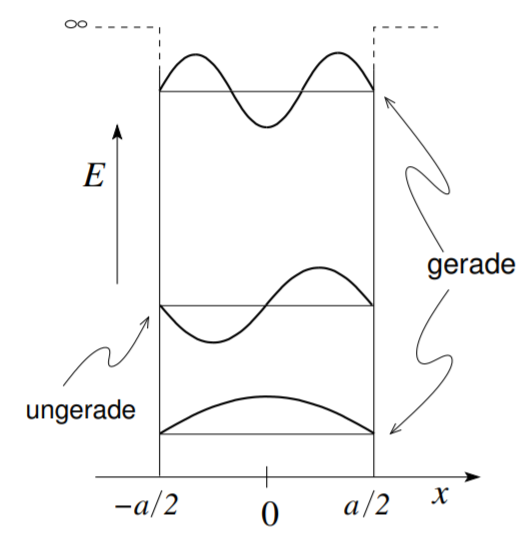
\includegraphics[scale=1]{1_18.PNG}
    \captionsetup{font={Large}}
    \caption{Conditions in the potential well with well-defined parity symmetry.}
    \label{fig:1.18}
\end{figure}
zero point in the middle. The system is characterized by the following Hamiltonian
description,
\\
\begin{equation}
\begin{aligned} H=-\frac{\hbar^{2}}{2 m} \partial_{x}^{2}+V_{\infty}(x) & \\ V_{\infty}(x) &=\left\{\begin{array}{ll}{0,} & {|x| \leq a / 2} \\ {\infty,} & {|x| \geq a / 2}\end{array}\right.\end{aligned}
\end{equation}\\
%公式 1.62
Again, one separates the problems in time and in place with the approach
\\
\begin{equation}
\Psi_{n}(x, t)=\chi_{n}(t) \varphi_{n}(x)
\end{equation}\\
%公式 1.63
we get the dynamic problem
\\
\begin{equation}
i \hbar \partial_{t} \chi_{n}=E_{n} \chi_{n}
\end{equation}\\
%公式 1.64
with the solution
\\
\begin{equation}
\chi_{n}=e^{-i \omega_{n} t}
\end{equation}\\
%公式 1.65
as well as the eigenvalue problem
\\
\begin{equation}
E_{n} \varphi_{n}=-\frac{\hbar^{2}}{2 m} \partial_{x}^{2} \varphi_{n}, \quad|x| \leq \frac{a}{2}
\end{equation}\\
%公式 1.66
with the boundary conditions
\\
\begin{equation}
\varphi_{n}(x) \equiv 0 \quad|x| \geq \frac{a}{2}
\end{equation}\\
%公式 1.67
%PAGE 41
The solutions are given by exponential functions $exp (\pm ikx)$, where
the allowed values ​​of $k$ are fixed by the boundary conditions,
\\\begin{equation}
k_{n}=n \frac{\pi}{a}
\end{equation}
\\
%gs 1.68
One finds solutions to even and odd $n$; these are odd resp.
straight in $x$,
\\
\begin{equation}
\varphi_{n}(x)=\left\{\begin{array}{ll}{\sin n \pi x / a,} & {n \geq 2, \quad \text { even }} \\ {\cos n \pi x / a,} & {n \geq 1, \quad \text { odd }}\end{array}\right.
\end{equation}\\
%公式 1.69
with the energies $E_n=\hbar^2 k_n^2/2m$(k-values ​​from the boundary conditions)
\\
\begin{equation}
E_{n}=\hbar \omega_{n}=\frac{\hbar^{2} k_{n}^{2}}{2 m}=\frac{\hbar^{2} \pi^{2}}{2 m a^{2}} n^{2}
\end{equation}\\
%公式 1.70
Again, the solution to the initial value problem is the superposition
\\
\begin{equation}
\Psi(x, t)=\sum_{n} a_{n} \Psi_{n}(x, t)
\end{equation}\\
%公式 1.71
given. For the initial condition to be fulfilled, must
\\
\begin{equation}
\begin{aligned} \Psi(x, 0)=& \sum_{n} a_{n} \Psi_{n}(x, 0) \\ & \stackrel{(1.59)}{\longrightarrow} a_{n}=\int d y \Psi(y, 0) \Psi_{n}^{*}(y, 0) \end{aligned}
\end{equation}\\
%公式 1.72
and thus one finds the following solution to the initial value problem,
\\
\begin{equation}
\Psi(x, t)=\int d y \sum_{n} \Psi_{n}^{*}(y, 0) \Psi_{n}(x, t) \Psi(y, 0)
\end{equation}\\
%公式 1.73
The propagator for the particle in the pot is
\\
\begin{equation}
\begin{aligned} K(x, t ; y, 0) &=\sum_{n} \Psi_{n}^{*}(y, 0) \Psi_{n}(x, t) \\ &=\sum_{n} \varphi_{n}^{*}(y) \varphi_{n}(x) e^{-i \omega_{n} t} \end{aligned}
\end{equation}\\
%公式 1.74
Of course, this solution strategy can also be applied to other problems
generalize, see later.
In the description of a free particle we note that plane
Waves basis $\Psi_k(x,t)$ is not normalizable. To mathematical problems
To avoid this, we must treat the wave functions more carefully; a
Possibility exists in the transition to wave packets, for example the
Gaussian wave packages.

%PAGE 42
\section{Gaussian Wave Packages}
Gaussian wave packages in place, i.e. Figure  1.19, describe particles in a localized state with finite extent $\triangle x$. Given that
Heisenberg Uncertainty Principle is the product $\triangle x\triangle k \sim 1$ fixed; a precise
localization in place then implies a broad distribution in the impulse (and
vice versa). Off the limes $\triangle x \to \infty$, the wave function is normalizable.
Mathematically, Gaussian wave packets are by expression
%Figure  1.19
\begin{figure}[ht]
    \centering
    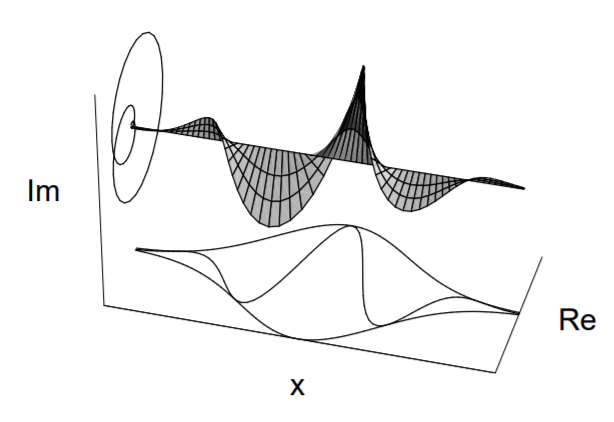
\includegraphics[scale=1]{1_19.PNG}
    \captionsetup{font={Large}}
    \caption{Gaussian wave package in the local area.}
    \label{fig:1.19}
\end{figure}
\\
\begin{equation}
\Psi(x, 0)=\frac{1}{\sqrt[4]{2 \pi \sigma}} e^{i k_{0} x} e^{-\left(x-x_{0}\right)^{2} / 4 \sigma}
\end{equation}\\
%公式 1.75
de ned. This form involves on the one hand the carrier $exp(ik_0x)$, on the other hand
the envelope end $exp[-(x-x_0)^2/4\sigma]$, as well as a normalization factor.
Even in $k$ space, the wavefunction has a Gaussian shape (and is therefore
normalizable for finite values ​​of $\sigma$),
\\
\begin{equation}
\begin{aligned} \Psi(k, 0) &=\mathcal{F}[\Psi(x, 0)]=\int d x \Psi(x, 0) e^{-i k x} \\ &=\sqrt[4]{8 \pi \sigma} e^{-i\left(k-k_{0}\right) x_{0}} e^{-\sigma\left(k-k_{0}\right)^{2}} \end{aligned}
\end{equation}\\
%公式 1.76
The propagation of a free massive particle is as usual via
the propagation of free plane waves with dispersion $E_k=\hbar^2 k^2/2m$,
\\
\begin{equation}
\begin{aligned} 
    \Psi(x, t) &=\int \frac{d k}{2 \pi} \Psi(k, 0) \exp \left[i\left(k x-\hbar k^{2} t / 2 m\right)\right] \\ 
    &=\sqrt[4]{8 \pi \sigma} \int \frac{d k}{2 \pi} e^{-i\left(k-k_{0}\right) x_{0}} e^{-\sigma\left(k-k_{0}\right)^{2}} e^{i\left(k x-\hbar k^{2} t / 2 m\right)}\\
    k \rightarrow & \underline{k+k_{0}} \sqrt[4]{8 \pi \sigma} e^{i k_{0} x} e^{-i \hbar k_{0}^{2} t / 2 m} \int \frac{d k}{2 \pi} e^{i k\left(x-\hbar k_{0} t / m-x_{0}\right)} e^{-i \hbar k^{2} t / 2 m} e^{-\sigma k^{2}} \\ 
    &=\sqrt[4]{\frac{\sigma}{2 \pi \sigma_{t}^{2}}} \underbrace{e^{i k_{0} x}} \underbrace{e^{i k_{0} x} e^{-i \hbar k_{0}^{2} t / 2 m}}_{\text {Phase }} e^{-\left(x-\hbar k_{0} t / m-x_{0}\right)^{2} / 4 \sigma_{t}} 
\end{aligned}
\end{equation}\\
%公式 1.77
%PAGE 43
with $\sigma_t=\sigma+i\hbar t/2m$. With the wave function (1.77) one finds the expectation values
\\
\begin{equation}
\begin{aligned}\langle x\rangle &= x_{0}+\frac{\hbar k_{0}}{m} t=x_{0}+v_{0} t \\\langle p\rangle &=\hbar\langle k\rangle=\hbar \int \frac{d k}{2 \pi} \Psi^{*}(k, 0) k \Psi(k, 0)=\hbar k_{0} \\(\Delta x)^{2} &=\left\langle\left(x-x_{0}-v_{0} t\right)^{2}\right\rangle= 2\left(\frac{1}{\sigma_{t}}+\frac{1}{\sigma_{t}^{*}}\right)^{-1}=\sigma\left(1+\frac{\hbar^{2} t^{2}}{4 m^{2} \sigma^{2}}\right) \\(\Delta p)^{2} &=\left\langle\left(p-\hbar k_{0}\right)^{2}\right\rangle=\frac{\hbar^{2}}{4 \sigma} \end{aligned}
\end{equation}\\
%公式 1.78
To determine $\triangle x^2$ we used a Gaussian distribution $\varpropto exp(-ax^2)$ has the width $\langle \triangle x^2 \rangle=1/2a$. With that we find the Zer
ow
of the wave packet linear in $t,\triangle x\varpropto t$, and the blur increases with time
to,
\\
\begin{equation}
\Delta x \Delta p=\frac{\hbar}{2} \sqrt{1+\frac{\hbar^{2} t^{2}}{4 m^{2} \sigma^{2}}} \geq \frac{\hbar}{2}
\end{equation}\\
%公式 1.79
Note that in Hamiltonian dynamics a packet is linear in time
cerium
If, $\triangle x\varpropto t$, the dissipative dynamics take a packet more slowly
cerium
asl, according to $\triangle x\varpropto \sqrt{t}$
\section{Location and momentum representation}
Let $f(\vec{r})\in \mathbb{C},\vec{r}\in\mathbb{R}^n$ given. The Fourier transformation
is a unit-is operation on the space of complex-valued functions.
Transferred to the space of the wave functions we get the representations
\\
\begin{equation}
\Psi(\vec{r}, t)=\int \frac{d^{n} p}{(2 \pi \hbar)^{n}} e^{i \vec{p} \cdot \vec{r} / \hbar} \Psi(\vec{p}, t)
\end{equation}\\
%公式 1.80
\\
\begin{equation}
\Psi(\vec{p}, t)=\int d^{n} r e^{-i \vec{p} \cdot \vec{r} / \hbar} \Psi(\vec{r}, t)
\end{equation}\\
%公式 1.81

%PAGE 44
\begin{equation}
\int d^{n} p e^{i \vec{p} \cdot \vec{r} / \hbar}=(2 \pi \hbar)^{n} \delta^{n}(\vec{r})
\end{equation}\\
%公式 1.82
interpretation
\{The plane wave $\phi_p=exp[i\vec{p}\cdot\vec{r}/\hbar]$, Eq. (1.57) describes a particle
with impulse $\vec{p}$. The impulse is sharp, according to the place unde -
($\phi_p$ can not be normalized, see later).
\{According to the superposition principle, (1.80) describes the function $\Psi(\vec{r},t)$
as superposition of partial waves $\phi_p$ with momentum $\vec{p}$.
From these two points one can conclude that $\Psi(\vec{p},t)$ the amplitude
of the particle at time t in the momentum space is the amplitude during $\Psi(\vec{x},t)$
of the particle in space).
It is
\\
\begin{equation}
|\Psi(\vec{r}, t)|^{2} d^{n} r
\end{equation}\\
%公式 1.83
the probability of the particle at time $t$ in volume $d^nr$ to $\vec{r}$
and analogously one interprets
\\
\begin{equation}
|\Psi(\vec{p}, t)|^{2} \frac{d^{n} p}{(2 \pi \hbar)^{n}}
\end{equation}\\
%公式 1.84
as the probability that the particle at time t the momentum in $d^np$
around \~{} p. We call
\\
\begin{equation}
\begin{array}{l}{\Psi(\vec{r}, t): \text { the wave function in spatial representation, }} \\ {\Psi(\vec{p}, t): \text { the wave function in pulse representation. }}\end{array}
\end{equation}\\
%公式 1.85
The Fourier transformation transforms between position and momentum representation,
the standardization is preserved,
\\
\begin{equation}
\int d^{n} r|\Psi(\vec{r}, t)|^{2} \quad \stackrel{\text { Parseval }}{=} \int \frac{d^{n} p}{(2 \pi \hbar)^{n}}|\Psi(\vec{p}, t)|^{2}
\end{equation}\\
%公式 1.86
Between these two representations a basic transformation--
We will discuss this in detail in the next chapter. At this point
Let us mention the different bases (location and momentum base with sharp
Location $\vec{r_0}$ and momentum $\vec{p}_0$) in the location (O-Dar) and momentum representations
(I-Dar) (note that these expressions are distributive or not normalizable):
\\
\begin{equation}
\begin{array}{ll}{\text { local base in O-Dar }} & {\Psi_{\vec{r}_{0}}(\vec{r})=\delta^{n}\left(\vec{r}-\vec{r}_{0}\right)} \\ {\text { pulse base in I-Dar }} & {\Psi_{\vec{p}_{0}}(\vec{p})=(2 \pi \hbar)^{n} \delta^{n}\left(\vec{p}-\vec{p}_{0}\right)}\end{array}
\end{equation}\\
%公式 1.87

%PAGE 45
\begin{equation}
\begin{array}{ll}{\text { Ipulse base in O-Dar }} & {\Psi_{\vec{p}_{0}}(\vec{r})=\int \frac{d^{n} p}{(2 \pi \hbar)^{n}} \Psi_{\vec{p}_{0}}(\vec{p}) e^{i \vec{p} \cdot \vec{r} / \hbar}=e^{i \vec{p}_{0} \cdot \vec{r} / \hbar}} \\ {\text { local base in } \mathrm{I}_{-} \mathrm{Dar}} & {\Psi_{\vec{r}_{0}}(\vec{p})=\int d^{n} r \Psi_{\vec{r}_{0}}(\vec{r}) e^{-i \vec{p} \cdot \vec{r} / \hbar}=e^{-i \vec{p} \cdot \vec{r}_{0} / \hbar}}\end{array}
\end{equation}\\
%
%公式 1.88
\newpage

%\chapter{Formalism of quantum mechanics}
\section{Hilbert space}
The validity of the superposition principle implies as a mathematical basis for the description of the QM a linear function space with scalar product (for normalization), generally a Hilbert space.
A Hilbert space $\mathcal{H}$ is defined as a set of abstract elements (vectors) $\phi,\psi$, we usually call them states, (The states in Hilbert space describe physical states (QM postulate)) with the following structures/properties:
\begin{enumerate}
    \item $\mathcal{H}$ is a linear (vector/functions) space, Pd.h. with $\phi_i\in\mathcal{H},a_i\in\mathbb{C}$ is also $\sum_ia_i\phi_i\in\mathcal{H}$.
    \item There exists a scalar product $\langle\cdot|\cdot\rangle$ with the properties
    %插入 公式
    $$
    \begin{aligned}
        -\phi, \psi & \in \mathcal{H},\langle\phi | \psi\rangle \in \mathbb{C}, \text { linear in } \psi, \text { antilinear in } \phi, \text { that is }( \text { with } \\
        & \left.a_{1}, a_{2} \in \mathbb{C}\right) \\
        & \left\langle a_{1} \phi_{1}+a_{2} \phi_{2} | \psi\right\rangle= a_{1}^{*}\left\langle\phi_{1} | \psi\right\rangle+ a_{2}^{*}\left\langle\phi_{2} | \psi\right\rangle \\
        & \left\langle\phi | a_{1} \psi_{1}+a_{2} \psi_{2}\right\rangle = a_{1}\left\langle\phi | \psi_{1}\right\rangle+ a_{2}\left\langle\phi | \psi_{2}\right\rangle\\
        -\langle\phi | \psi\rangle & =\langle\psi | \phi\rangle^{*} \text { ist hermitesch. } \\
        -\langle\phi | \phi\rangle & \geq 0 ; \text { falls }\langle\phi | \phi\rangle= 0 \text { ist } \phi \equiv 0 
    \end{aligned}
    $$
    \item $\mathcal{H}$ is completely constant, that is, for every convergent sequence $\phi_n$ with $\phi_n\in\mathcal{H}$ applies $\lim_{n\to\infty}\in\mathcal{H}$ (a sequence $\phi_n$ is called convergent if $\parallel\phi_n-\phi_m\parallel\to0$ for $n,m\to\infty$ where $\parallel\phi\parallel^2\equiv\langle\phi|\phi\rangle$).\\ One also often requires:
    \item $dim\mathcal{H} = \infty$, which means that there are $\infty$ many linearly independent elements in $\mathcal{H}$. Otherwise one speaks of a finite-dimensional Hilbert space.
    \item $\mathcal{H}$ separable, i.e. there is a countable set ${\psi_n}\in\mathcal{H}$, so that every $\phi\in\mathcal{H}$ can be arbitrarily approximated by elements from ${\psi_n}$.
\end{enumerate}

Two examples are mentioned:
\begin{enumerate}
    \item[-] Complex vector space, a finite-dimensional Hilbert space with finitely many basis vectors.
    \item[-] Space of square integrable functions L2 (Rn), a 1-dimensional vector space. This is the typical Hilbert space we consider in quantum mechanics.
\end{enumerate}

\subsection{Scalar Product}
With the aid of the scalar product, we define the norm of $\phi\in\mathcal{H}$ as
%公式 2.1
\begin{equation}
    \|\phi\| \equiv\langle\phi | \phi\rangle^{1 / 2}
\end{equation}
The scalar product of two states satisfies the following inequalities: S Black's inequality: Let $\phi,\psi\in\mathcal{H}$, then hold
%公式 2.2
\begin{equation}
    |\langle\phi | \psi\rangle|^{2} \leq\langle\phi | \phi\rangle\langle\psi | \psi\rangle
\end{equation}
Triangle inequality: Let $\phi,\psi\in\mathcal{H}$, then hold
%公式 2.3
\begin{equation}
    \|\phi+\psi\| \leq\|\phi\|+\|\psi\|
\end{equation}
$\langle\phi|\psi\rangle$ and $\langle\phi,\psi\rangle$ are equivalent notations. In the space of the square integrable functions $\phi(\vec{r})\in\mathbb{C},\vec{r}\in\mathbb{R}^n$, the scalar product (of $\psi,\phi\in\mathcal{H}$ is defined by
%公式 2.4
\begin{equation}
    \langle\psi, \phi\rangle=\int d^{n} r \psi^{*}(\vec{r}) \phi(\vec{r})
\end{equation}

%Page 51
\section{vectors/states}
A state $\phi\in\mathcal{H}$ is called normalized if
%公式 2.5
\begin{equation}
    \|\phi\|=1
\end{equation}
For $\psi\in\mathbb{L}_2$ (that is, $\psi$ is square integrable), $\psi$ is normalizable, $\psi\to\psi/\parallel\psi\parallel$. We define the orthogonality of $\phi,\psi\in\mathcal{H}$ as
%公式 2.6
\begin{equation}
    \langle\phi | \psi\rangle= 0 \leftrightarrow \phi \text { is orthogonal to } \psi
    \end{equation}
\subsection{Orthonormation and completeness}
A set {$\phi_n$}, $\phi_n\in\mathcal{H}$ is called orthonormal if
%公式 2.7
\begin{equation}
    \left\langle\phi_{m}, \phi_{n}\right\rangle=\delta_{m n}
    \end{equation}
A set {$\psi_n$} $\in\mathcal{H}$ ($\mathcal{H}$ separable) is called completely if every $\psi\in\mathcal{H}$ can be represented by the {$\psi_n$},
%公式 2.8
\begin{equation}
    \psi=\sum_{n} c_{n} \psi_{n}
    \end{equation}
A system of states ${\psi_n}\in\mathcal{H}$ is called complete and orthonormal (vONS) if (2.7) and (2.8) are satisfied. This system is called a Ba¨sis in Hilbert space $\mathcal{H}$ (or {$\psi_n$} spans $\mathcal{H}$). For a set of orthonormal functions ${\psi_n(x)}\subset\mathbb{L}_2$, the completeness can be expressed
%公式 2.9
\begin{equation}
    \sum_{n} \psi_{n}^{*}(y) \psi_{n}(x)=\delta(x-y)
    \end{equation}
then functions $\phi(x)\in\mathbb{L}_2$ can be represented as
%公式 2.10
\begin{equation}
\begin{aligned} \phi(x) &=\int d y \delta(x-y) \phi(y)=\int d y \sum_{n} \psi_{n}^{*}(y) \psi_{n}(x) \phi(y) \\ &=\sum_{n}\left\langle\psi_{n}, \phi\right\rangle \psi_{n}(x)=\sum_{n} c_{n} \psi_{n}(x) \end{aligned}
\end{equation}
In general, for an orthonormal system (ONS), Bessel's inequality holds,
%公式 2.11
\begin{equation}
    \sum_{n}\left|c_{n}\right|^{2}=\sum_{n}\left\langle\phi, \psi_{n}\right\rangle\left\langle\psi_{n}, \phi\right\rangle \leq\langle\phi, \phi\rangle
    \end{equation}
for a vONS, in (2.11) using inequality $\leq$ instead of  equality =.

%Page 52
\subsection{Schmidt's orthogonalization method}
Let {$\phi_n$} be a set of elements in $\mathbb{L}_2(\mathbb{R}^n)$. We construct an orthonormal system
%公式 2.12
\begin{equation}
    \psi_{1} \equiv \phi_{1} /\left\|\phi_{1}\right\|
    \end{equation}
%公式 2.13
\begin{equation}
\begin{array}{l}
{\left\{\begin{array}{ll}{h_{2}=} & {\phi_{2}-\left\langle\psi_{1}, \phi_{2}\right\rangle \psi_{1}} \\ 
{\psi_{2}=} & {\left.h_{2} / \| h_{2}\right\rangle \psi_{1}}\end{array}\right.} \\ 
\vdots\\
{\left\{
    \begin{array}{ll}
        {h_{n}} & {=\phi_{n}-\sum_{k=1}^{n-1}\left\langle\psi_{k}, \phi_{n}\right\rangle \psi_{k}} \\ 
        {\psi_{n}} & {=h_{n} /\left\|h_{n}\right\|}\end{array}\right.}
    \end{array}
\end{equation}
\section{operators}
A linear operator $A$ on $\mathcal{H}$ is a linear mapping from $\mathcal{H}$ to $\mathcal{H}$,
%公式 2.14
\begin{equation}
\begin{array}{ll}{A:} & {\mathcal{H} \rightarrow \mathcal{H}} \\ {A:} & {\phi \in \mathcal{H} \rightarrow A \phi \in \mathcal{H}}\end{array}
\end{equation}
%公式 2.15
\begin{equation}
\begin{array}{ll}{\phi, \psi \in \mathcal{H},} & {a, b \in \mathbb{C}} \\ {A \text { linear : }} & {A(a \phi+b \psi)=a A \phi+b A \psi}\end{array}
\end{equation}
\subsection{Example: Pulse operator}
Task: Compute $\langle\vec{p}\rangle$ in the location representation:
%公式 2.16
\begin{equation}
\begin{aligned}\langle\vec{p}\rangle &=\int \frac{d^{n} p}{(2 \pi \hbar)^{n}} \psi^{*}(\vec{p}, t) \vec{p} \psi(\vec{p}, t) \\ &=\int \underbrace{d^{n} r d^{n} r^{\prime}} \int \frac{d^{n} p}{(2 \pi \hbar)^{n}} \underbrace{e^{i \vec{p} \cdot \vec{r}^{\prime} / \hbar} \psi^{*}\left(\vec{r}^{\prime}, t\right)}_{\psi^{*}(\vec{p}, t)} \vec{p} \underbrace{e^{-i \vec{p} \cdot \vec{r} / \hbar} \psi(\vec{r}, t)}_{\psi(\vec{p}, t)} \\ & \downarrow \vec{p} e^{-i \vec{p} \cdot \vec{r} / \hbar} \psi=\left(-\frac{\hbar}{i} \nabla e^{-i \vec{p} \cdot \vec{r} / \hbar}\right) \psi^{\text {part.Int. }}= e^{-i \vec{p} \cdot \vec{r} / \hbar} \frac{\hbar}{i} \nabla \psi \\ &=\int d^{n} r \psi^{*}(\vec{r}, t)\left[\frac{\hbar}{i} \nabla \psi(\vec{r}, t)\right] \end{aligned}
\end{equation}
%Page 53
The momentum operator in the location representation is (see page 38)
%公式 2.17
\begin{equation}
    \vec{p}=-i\hbar\nabla
\end{equation}
\subsection{General Definitions \& Properties}
We define the following terms:
\begin{enumerate}
    \item[-] $A$ is linear if          $A\sum_ia_i\psi_i=\sum_ia_iA\psi_i$ for ¨ $a_i \in \mathbb{C}$.
    \item[-] $A^{\dagger}$ is the adjoint to $A$ if $\langle A^{\dagger}\phi,\psi=\langle\phi,A\psi\rangle,\forall\phi,\psi\in\mathbb{L}_2$.
    \item[-] $A$ is Hermitian (physical observables correspond to Hermitian operators (QM postulate).) (self-adjoint) if $A=A^{\dagger}$. It holds: $(AB)^{\dagger}=B^{\dagger}A^{\dagger}$.
\end{enumerate}
Examples of linear Hermitian operators are:
\begin{enumerate}
    \item[-] $\vec{r}$, multiplication with $\vec{r}$, the location operator.
    \item[-] $\vec{p}$, derivative $-i\hbar\nabla$, the momentum operator.
    \item[-] $\mathcal{H}$, the Hamiltonian.
    \item[-] $f(\vec{r})$, multiplication by $f(\vec{r}),f:\mathbb{R}^n\to\mathbb{R}^n$, e.g. $V(\vec{r})$.
    \item[-] $g(\vec{p})$, like $f(\vec{r})$ but in momentum space, or $g(\vec{r}),=\sum_n\frac{g^{(n)}}{n!}(-i\hbar\nabla)^n$ in space if a Taylor series exists.
\end{enumerate}

While products from operators $x_n$ or $p_n$ are easy to handle, we need to be careful with mixed products, such as $xp$; although $x$ and $p$ are hermich this is no longer true for the product $xp$: it is $(xp)^{\dagger}=p^{\dagger}x^{\dagger}=px$ and applying to a function $\psi(x)$ yields
%公式2.18
\begin{equation}
\begin{aligned} p x \psi(x) &=-i \hbar \partial_{x}(x \psi)=-i \hbar\left(\psi+x \psi^{\prime}\right) \\ x p \psi(x) &=x\left(-i \hbar \partial_{x}\right) \psi=-i \hbar x \psi^{\prime} \end{aligned}
\end{equation}
$\Rightarrow xp-px=i\hbar$ (as an operator identity). Thus, with $\vec{r}$ also $f(\vec{r})$, with $\vec{p}$ also $g(\vec{p})$ hermitian, but a mixed product of Hermitian operators (for example, $h(\vec{r}\dot\vec{p})$) does not lead to a new Hermitian operator. You can hermitize xp,
%公式 2.19
\begin{equation}
    \frac{1}{2}(xp+px)
\end{equation}

%Page 54
\subsection{commutator}
Let $A$ and $B$ be linear operators. Then means
%公式 2.20
\begin{equation}
    [A,B]=AB-BA \text{Commutator from} A \text{ with } B
\end{equation}
Examples of commutators:
%公式
$$
    [x_i,p_k]=i\hbar \delta_{ik}; \\i=k \text{ are (canonical) conjugate variables}\\
    \left.
    \begin{array}{l}{\left[x_{i}, x_{j}\right]=0} \\ {\left[p_{i}, p_{j}\right]=0}
    \end{array}\right\}\text{Operator commute}
$$
\subsection{Useful identities}
%公式 2.21
\begin{equation}
\begin{array}{l}{[A B, C]=A[B, C]+[A, C] B} \\ {[A, B]^{\dagger}=\left[B^{\dagger}, A^{\dagger}\right]}\end{array}
\end{equation}
Baker-Hausdorff: with $exp[A]=\sum^{\infty}_{n=0}A^n/n!$ applies
%公式 2.22
\begin{equation}
    e^{A} B e^{-A}=B+[A, B]+\frac{1}{2}[A,[A, B]]+\cdots
    \end{equation}
If $[A, B]$ commutes with $A$ and $B$, then $[[A, B], A] = [[A, B], B] = 0$, especially if $[A, B] \in \mathbb{C}$, then
%公式 2.23
\begin{equation}
    e^{A} e^{B}=e^{B} e^{A} e^{[A, B]}, \quad e^{A+B}=e^{A} e^{B} e^{-[A, B] / 2}
    \end{equation}
\subsection{Expected values}
Given a state $\psi\in\mathcal{H}$ and a (hermitian) operator $A$. We define
%公式 2.24
\begin{equation}
\begin{aligned}
\langle A\rangle &=\langle\psi, A \psi\rangle=\int d^{n} r \psi^{*}(r) A \psi(r) \text { the expected value of } A \\\langle\Delta A\rangle &=\left\langle(A-\langle A\rangle)^{2}\right\rangle^{1 / 2} \\ \&=\left(\left\langle A^{2}\right\rangle-\langle A\rangle^{2}\right)^{1 / 2} \text { the fluctuation of } A \end{aligned}
\end{equation}
%Page 55
\subsection{Component decomposition of $A\psi$}
$\phi$ means orthogonal to $\psi$ if $\langle\phi,\psi\rangle=0$. We denote by $\psi_{\bot}$ an orthogonal function to $\psi$. Let $A$ be Hermitesh, $\psi_{\bot}$ normalized, $\parallel\psi_{\bot}\parallel=1$, then let $A\psi$ be dismantled
%公式 2:25
\begin{equation}
\begin{array}{c}{A \psi=\langle A\rangle_{\psi} \psi+\langle\Delta A\rangle_{\psi} \psi_{\perp}} \end{array}
\end{equation}
(Note: For $A\psi\neq\langle A\rangle\psi, \psi_{\bot}=(A-\langle A\rangle)\psi/\parallel(A-\langle A\rangle)\psi\parallel$/)
\subsection{operators with discrete spectrum}
Let $A$ be a linear operator and $\psi_n$ fill
%公式 2.26
\begin{equation}
    A\psi_n=a_n\psi_n, a_n\in \mathbb{C}
\end{equation}
$a_n$ eigenvalue of $A$, $\psi_n$ is the associated eigenvector. The (discrete)
Set ${a_n}$ means (discrete) spectrum of $A$.
Let $A$ be Hermitian, then $a_n=a_n^*\Rightarrow a_n\in\mathbb{R}$, that is, the spectrum (the
Eigenvalues) of Hermitian operators is (are) real.
Let $a_n\neq a_m$, then the associated eigenvectors are orthogonal, $\langle \psi_n, \psi_m\rangle=0$ or $\psi_n \bot\psi_m$.
Let $a_n=a_m$ degenerate eigenvalue, then let the corresponding ones be orthogonalize eigenvectors {$\psi_n$}: we define the matrix elements
%公式 2.27
\begin{equation}
    \left\langle\psi_{m}, \psi_{n}\right\rangle= C_{m n}=C_{n m}^{*}
    \end{equation}
$C_{mn}$ is Hermitian, so $\exists U_{nm},U$ is unitary, so that $U_{m\alpha}^*C_{mn}U_{n\beta}=c_{\alpha}\delta_{\alpha\beta}$ is diagonal. Then $\varphi_{\alpha}=\mathcal{X}_{\alpha}/\parallel\mathcal{X}_{\alpha}\parallel$ with $\mathcal{X}_{\alpha}=U_{n\alpha}\psi_n$, orthonormated (see also Schmidt's Orthogonalisierungsverfahren).
We can conclude that a system of eigenvectors {$\psi_n$} for a Hermitian operator can always be orthonormalized, $\langle\psi_m,\psi_n\rangle=\delta_{mn}$. In addition, the eigensystem {$\psi_n$} becomes a hermitian operator with discrete spectrum complete; such an operator always defines a vONS (a base in Hilbert space).
\subsection{Operators with continuous spectra}
Example: We consider the operators $x, p$ on $\mathbb{L}_2(\mathbb{R})$ (Warning: this
Considerations do not claim mathematical rigor).
%Page 56
The eigenfunctions to $x, p$ are not regular (see page 44)
%公式 2.28
\begin{equation}
\begin{aligned} x \psi_{x_{0}}(x) &=x_{0} \psi_{x_{0}}(x), & & \psi_{x_{0}}(x)=\delta\left(x-x_{0}\right) \\ p \psi_{p_{0}}(x) &=p_{0} \psi_{p_{0}}(x), & & \psi_{p_{0}}(x)=\frac{e^{i p_{0} x / \hbar}}{\sqrt{2 \pi \hbar}} \end{aligned}
\end{equation}
$\psi_{x0}(x)$ is a distribution, $\psi_{p0}(x)$ is not normable. Accordingly, we need distributions and integrals (Mass!) Instead of sums to formulate the orthogonality and completeness.\\
Now let {$\psi_a$} be an eigensystem to $A,A\psi_a=a\psi_a$.\\\\
\textbf{Orthogonality} The set of functions {$\psi_a$} is orthogonal if
%公式 2.29
\begin{equation}
    \int d x \psi_{a_{1}}^{*}(x) \psi_{a_{2}}(x)=\delta\left(a_{1}-a_{2}\right), \quad a=x_{0}, p_{0}, \cdots
    \end{equation}
\textbf{Completeness} The set of functions {$\psi_a$} is complete when
%公式 2.30
\begin{equation}
    \int d a \psi_{a}^{*}(y) \psi_{a}(x)=\delta(x-y), \quad a=x_{0}, p_{0}, \cdots
    \end{equation}
A hermitian operator (for example, $x$ or $p$) again produces a complete system {$\psi_a$}. A clean formulation can be given with the spectral representation of the operators.\\\\
\textbf{Development} according to $\psi_a(x)$ every function $\phi$ can be developed into {$\psi_a$},
%公式 2.31
\begin{equation}
\begin{aligned} \phi(x) &=\int d y \delta(x-y) \phi(y)=\int d a \int d y \psi_{a}^{*}(y) \psi_{a}(x) \phi(y) \\ &=\int d a\left\langle\psi_{a}, \phi\right\rangle \psi_{a}(x)=\int d a c(a) \psi_{a}(x) \end{aligned}
\end{equation}
Continuous and discrete spectra are quite different:
%公式 2:32
\begin{equation}
\begin{array}{l}{\text { Continuous spectra } \longleftrightarrow \text { Discrete spectra }} \\ {\qquad \begin{aligned} c(a)=\left\langle\psi_{a}, \phi\right\rangle & \stackrel{(2.10)}{\longrightarrow} c_{n}=\left\langle\psi_{n}, \phi\right\rangle \\ \int d a \cdots & \longleftrightarrow \sum_{n} \cdots \end{aligned}}\end{array}
\end{equation}
%Page 57
In general, there may be operators with mixed spectra, partly discrete, partly continuous (for example, bound and scattering states of a Hamiltonian $H=p^2/2m+V(\vec{r})$ with attractive potential V).
\textbf{Remark}, for the operators $x$ and $p$ (Eig $x$ = eigenvalue to the operator $x$)
%公式 2:33
\begin{equation}
\begin{aligned} \phi(x) &=c(a) \text { for } a \in \operatorname{Eig} x \\ \phi(p) &=c(a) \text { for } a \in \operatorname{Eig} p \end{aligned}
\end{equation}
Thus, $\phi(x)$ and $\phi(p)$ are the development coefficients if the vONS of the operators $x\&p=-i\hbar\partial_x$ are chosen as the basis (eg, for $a=x_0,c(x_0)=\langle\psi_{x0},\phi\rangle=\int dx\delta(x_0-x)\phi(x)=\phi(x_0)$).
\subsection{Matrix representation of an operator}
Let {$\phi_n$}, $\phi_n\in\mathcal{H}$ be a basis in $\mathcal{H}$, $A$ be a (Hermitian) operator on $\mathcal{H}$, then $A$ can be represented in this basis via the matrix
%公式 2:34
\begin{equation}
    A_{n m}=\left\langle\Psi_{n}, A \Psi_{m}\right\rangle= A_{m n}^{*}
    \end{equation}
\section{Observable and correspondence principle}
We combine the mathematical structures developed above with physical contents; the complex functions $\phi$ now become wave functions $\psi$, the operators become observables: a measure of classical physics, e.g. the place, the momentum, the energy or the angular momentum corresponds in quantum mechanics to a hermitian operator $\to$ observables in quantum mechanics are Hermitian operators. The assignment of the classical measuring quantities to the quantum mechanical observables regulates the correspondence principle:
\begin{enumerate}
    \item[-] Quantum mechanics assign (hermitian) operators to physical variables (QM postulate).
    \item[-] The classical relations correspond to quantum mechanical relations.
\end{enumerate}
%Page 58
The following mappings and relations are consistent:
$$
\begin{array}{cl}{\text { Position } \vec{r}} & {\longrightarrow \vec{r}} \\ {\text { Impulse } \vec{p}} & {\longrightarrow-i \hbar \nabla} \\ {\text { Energy } E} & {\longrightarrow i \hbar \partial_{t}} \\ {\text { for the classic track applies: }} & {E=\frac{p^{2}}{2 m}+V(\vec{r})} \\ {\text { for the qm wavefunction: }} & {i \hbar \partial_{t} \Psi(\vec{r}, t)=\left[-\frac{\hbar^{2}}{2 m} \nabla^{2}+V(\vec{r})\right] \Psi(\vec{r}, t)}\end{array}
$$
Remarks: i) The relation $i\hbar\partial_t=-(\hbar^2/2m)\nabla^2+V$ does not apply as an operator identity but applies to a quantum mechanical wave function $\psi$. ii) Generalization: Consider the classical Hamiltonian function $H(\vec{p},\vec{q})$; the classical relation $E=H(\vec{p}_{kl},\vec{q}_{kl})$ holds for the orbit $\vec{p}_{kl},\vec{q}_{kl}$.
In quantum mechanics we have the corresponding Hermitian $H(-i\hbar\nabla,\vec{q}),H=H^{\dagger}$, and the equation of the equation applies
%公式 2:35
\begin{equation}
    i\hbar \partial_t\Psi=H\Psi
\end{equation}
\subsection{Honorary Theorem}
The Ehrenfest theorem states that the mean values ​​of an observable satisfy the classical equations ($\nrightarrow$ classical equations of motion for $\langle x\rangle$ and $\langle p\rangle$, see later). We construct the dynamic equations for the mean $\langle A\rangle$ of operator $A$ as follows:
%公式 2:36
\begin{equation}
\begin{array}{l}{\text { Schrodinger equation }(\mathrm{SG}): \quad i \hbar \partial_{t} \Psi=H \Psi} \\ {\text { SG complex conjugate }:-i \hbar \partial_{t} \Psi^{*}=H \Psi^{*}} \\ {\text { Observable : } A} \\ {\qquad \begin{aligned} \text { Observable } &: A \\ \text { Dynamic for }\langle A\rangle &=\int d^{n} r \Psi^{*}(\vec{r}, t) A \Psi(\vec{r}, t): \\ \frac{d}{d t}\langle A\rangle &=\int d^{n} r\left[\left(\partial_{t} \Psi^{*}\right) A \Psi+\Psi^{*}\left(\partial_{t} A\right) \Psi+\Psi^{*} A\left(\partial_{t} \Psi\right)\right] \\ &=\frac{i}{\hbar}\langle[H, A]\rangle+\left\langle\partial_{t} A\right\rangle \end{aligned}}\end{array}
\end{equation}
The Ehrenfest Theorem of classical mechanics states that
%公式 2:37
\begin{equation}
    \frac{d}{d t} f(p, q, t)=\{H, f\}+\partial_{t} f
\end{equation}
%Page 59
with the Poisson brackets ${H,f}=(\partial_p H)(\partial_q f)-(\partial_p f)(\partial_q H)$, where $\partial_x=d/dx$. The comparison of (2.36) with (2.37) yields the correspondence
%公式 2:38
\begin{equation}
    {f,g}\leftrightarrow\frac{i}{\hbar}[F,G],
\end{equation}
where the sizes $f\leftrightarrow F$ and $g\leftrightarrow G$ correspond to the observables.
Example: Particles in potential $V(\vec{r})$
%公式 2:39
\begin{equation}
\begin{array}{l}{A=\vec{r} \longrightarrow[H, \vec{r}]=\left[\vec{p}^{2} / 2 m, \vec{r}\right]=-i \hbar \vec{p} / m} \\ {A=\vec{p} \longrightarrow[H, \vec{p}]=[V(\vec{r}), \vec{p}]=i \hbar \nabla V}\end{array}
\end{equation}
thus follows
%公式 2:40
\begin{equation}
\left.\begin{array}{rl}{\frac{d}{d t}\langle\vec{r}\rangle} & {=\langle\vec{p}\rangle / m} \\ {\frac{d}{d t}\langle\vec{p}\rangle} & {=-\langle\nabla V(\vec{r})\rangle} \\ { m \frac{d^{2}}{d t^{2}}\langle\vec{r}\rangle} & {=-\langle\nabla V(\vec{r})\rangle}\end{array}\right\} \text { Ehrenfest theorem. }
\end{equation}
However, it does not hold that $m\partial_t^2\langle\vec{r}\rangle=-\nabla V(\langle\vec{r}\rangle)$; the expectation $\langle x\rangle$ does not follow the classical trajectory since $\langle\nabla V(\vec{r})\rangle\neq\nabla V(\langle\vec{r}\rangle)$ (the corrections are given by $\vec{r}=\langle\vec{r}\rangle + (\vec{r}-\langle\vec{r}\rangle)$ and subsequent development by $\langle \vec{r}\rangle$).
\subsection{Probabilistic densities and continuity equation}
The interpretation of
%公式 2:41
\begin{equation}
    \rho(\vec{r})\Psi^*(\vec{r})\Psi(\vec{r})
\end{equation}
as probability density leads to the question of the definition of probability current density $\vec{j}(\vec{r})$. The following consideration applies to one Hamiltonian of type $H=p^2/2m+V(\vec{r})$. Let $\rho=\Psi^*(\vec{r},t)\Psi(\vec{r},t)$ the
Probability density, then is
%公式 2:42
\begin{equation}
\begin{aligned} \partial_{t} \rho &=\left(\partial_{t} \Psi^{*}\right) \Psi+\Psi^{*}\left(\partial_{t} \Psi\right) \\ & \stackrel{\mathrm{S}_{\mathrm{G}}}{=} \frac{-1}{i \hbar}\left(H \Psi^{*}\right) \Psi+\frac{1}{i \hbar} \Psi^{*}(H \Psi) \\ &=\frac{\hbar}{2 m i}\left[\left(\nabla^{2} \Psi^{*}\right) \Psi-\Psi^{*}\left(\nabla^{2} \Psi\right)\right] \\
&=-\frac{\hbar}{2 m i} \nabla \cdot\left(\Psi^{*} \nabla \Psi-\Psi \nabla \Psi^{*}\right) \\ &\downarrow \quad \vec{j} \equiv \frac{\hbar}{2 m i}\left(\Psi^{*} \nabla \Psi-\Psi \nabla \Psi^{*}\right) \\ &=-\nabla \cdot \vec{j}\end{aligned}
\end{equation}
\\
%Page 60
Thus the continuity equation holds
%公式 2:43
\begin{equation}
    \partial_t\rho+\text{div}\vec{j}=0
\end{equation}
if we define the current density $\vec{j}$ via (2.42).\\\\
Remarks: 
\begin{enumerate}
    \item[-] $\vec{j}$ is defined such that with $i\hbar\partial_t\Psi=H\Psi$ the continuity equation holds and the dynamics does not generate any particle loss. Thus we have a method with known probability density $\rho(\Psi)$ and Hamiltonian $H$ to find the probability current density $\vec{j}(\Psi)$.
    \item[-] Let $\Psi=\sqrt{\rho(\vec{r},t)}exp[i\varphi(\vec{r},t)]$ represented by amplitude and phase. Then $\vec{j}=(\hbar/m)\rho(\vec{r},t)\nabla\varphi(\vec{r},t)$, the particle flow, only when $\neq 0$, if $\Psi$ has a location-dependent phase $\varphi(\vec{r},t)$. It is the phase gradient which drives the currents (compare with Ohm's law in the electrodynamics, where a particle stream in the material usually is driven by a electric field).
\end{enumerate}
\subsection{Stationary states and evolution}
If $\partial_t H=0, H$ is time-independent, then we can separate the dynamics,
%公式 2:44
\begin{equation}
\begin{aligned}  \text{ with } i \hbar \partial_{t} \Psi=H \Psi \text{ applies }\left\{\begin{aligned}\Psi(\vec{r}, t) &=\chi(t) \varphi(\vec{r})\\ \chi(t) &=\exp [-i E t / \hbar] \\ H \varphi(\vec{r}) &=E \varphi(\vec{r}) \end{aligned}\right.\end{aligned}
\end{equation}
the position-dependent component $\varphi(\vec{r})$ is the solution of the time-independent Schrodinger equation $H\varphi = E\varphi$, an eigenvalue problem which is under consideration of the boundary condition. $\Psi(\vec{r},t)=e^{-iEt/\hbar}\varphi(\vec{r})$Stationary state, the associated density $\rho=|\Psi|^2=|\varphi|^2$is time-independent. The boundary condition/normalization condition of the eigenvalue problem $H\varphi_n=E_n\varphi_n$ specifies the allowed energies $E_n$.\\\\
The time-independent Schrodinger equation defines a useful vONS {$\varphi_n$}: The time evolution of a general state $\Psi(\vec{r},t)$ with initial value $P_{si}(\vec{r},t=0)=\Psi_0(\vec{r})$ results from the decomposition vin $\Psi_0$ into components
%公式 2:45
\begin{equation}
    \Psi_{0}(\vec{r})=\sum\left\langle\varphi_{n}, \Psi_{0}\right\rangle \varphi_{n}(\vec{r})
    \end{equation}
and their individual evolutions with the energies $E_n$ (compare with the discussion in section 1.6)
%公式 2:46
\begin{equation}
    \Psi(\vec{r}, t)=\sum_{n}\left\langle\varphi_{n}, \Psi_{0}\right\rangle \varphi_{n}(\vec{r}) e^{-i E_{n} t / \hbar}
    \end{equation}
\section{measuring process}
In quantum mechanics, we can determine only one distribution function $w (a)$ for the measurement of an observable; the quantities $w (a) da$ gives the probability of finding a measured value a in the interval $[a, a + da]$. The distribution function $w (a)$ is defined in quantum mechanics by the observable $A$ and the state $\Psi$ of the system. Probably, a measurement process {$A,\Psi$} corresponds to a random variable $A$, which takes values ​​a according to $w (a)$. We define
%公式 2:47
\begin{equation}
    m_{n} \equiv \int d a a^{n} w(a)
    \end{equation}
as the $n^{tes}$ moment of $w (a)$, and
%公式 2:48
\begin{equation}
    \chi(\tau)=\mathcal{F}_{\tau}(w)=\int d a e^{-i a \tau} w(a)
    \end{equation}
as a characteristic function, the Fourier transform of the distribution function $w (a)$. The characteristic function $\mathcal{X}(tau)$ gives all moments $m_n$ of the distribution function,
%公式 2:49
\begin{equation}
    m_{n}=i^{n} \frac{d^{n} \chi}{d \tau^{n}}
    \end{equation}
Thus $w (a)$ can be determined from the moments $m_n$
%公式 2:50
\begin{equation}
\begin{aligned} \chi(\tau) &=\sum_{n=0}^{\infty} \frac{(-i \tau)^{n}}{n !} m_{n} \\ w(a) &=\int_{-\infty}^{\infty} \frac{d \tau}{2 \pi} e^{i a \tau} \chi(\tau) \end{aligned}
\end{equation}
%page 62
\textbf{Note}, often the cumulants $c_k$ are used instead of the moments,
%公式 2:51
\begin{equation}
\begin{aligned} \sum_{n} \frac{x^{n}}{n !} m_{n} &=\exp \left[\sum_{k} \frac{x^{k}}{k !} c_{k}\right] \\ c_{1} &=m_{1} \\ c_{2} &=m_{2}-m_{1}^{2} \\ c_{3} &=m_{3}-3 m_{2} m_{1}+2 m_{1}^{3} \\ c_{4} &=m_{4}-4 m_{3} m_{1}-3 m_{2}^{2}+12 m_{2} m_{1}^{2}-6 m_{1}^{4} \\ \ldots &=\cdots \end{aligned}
\end{equation}
Application to the quantum mechanical measuring process {$A,\Psi$}:
\begin{enumerate}
    \item[-] Let $\Psi=\Psi_n$ be an eigenstate of $A$, $A\Psi_n=a_n\Psi_n$. The expected value $\langle A\rangle$ is equal to the physical mean of the measurement results over many equivalent measurements {$A,\Psi$}; same for the moments    (QM postulate). Then $\langle A^k\rangle=a_n^k$ the $k_{th}$ moment,%公式 2:52
    \begin{equation}
    \begin{aligned} \chi(\tau) &=\sum_{k} \frac{(-i)^{k}}{k !}\left(a_{n} \tau\right)^{k}=\exp \left(-i a_{n} \tau\right) \\ w(a) &=\int_{-\infty}^{\infty} \frac{d \tau}{2 \pi} e^{i a \tau} e^{-i a_{n} \tau}=\delta\left(a-a_{n}\right) \end{aligned}
    \end{equation}
    and it is certainly measured, since the measurement is a pure state with an eigenfunction.
    \item[-] Let $\Psi=\sum_n c_n\Psi_n$ a superposition, then the $k_{th}$ moment
    \begin{equation}
    \begin{aligned}\left\langle A^{k}\right\rangle &=\sum_{n}\left|c_{n}\right|^{2} a_{n}^{k} \\ \chi(\tau) &=\sum_{n}\left|c_{n}\right|^{2} e^{-i a_{n} \tau} \\ w(a) &=\sum_{n}\left|c_{n}\right|^{2} \delta\left(a-a_{n}\right) \end{aligned}
    \end{equation}
    that is, it is measured with the probability $| c_n|^2$ of the eigenvalue $a_n$.
\end{enumerate}
%公式 2:53
%Page 63
\textbf{In summary}, let {$\Psi_n$} be a vONS to $A$ with (discrete) spectrum {$a_n$} (continuous parts in the spectrum are treated according to (2.32)). Every state of a system can be written as
%公式 2:54
\begin{equation}
    \Psi=\sum_{n} c_{n} \Psi_{n}, \quad\|\Psi\|^{2}=\sum_{n}\left|c_{n}\right|^{2}=1
    \end{equation}
The measurement of observable $A$ on the system in state $\Psi$ shows that
\begin{enumerate}
    \item[-] with probability $| c_n|^2$ the eigenvalue $a_n$ is measured (Born), in particular only eigenvalues ​​are measured,
    \item[-] after the measurement of the eigenvalue $a_n$, the system is in the state $\Psi_n$ (von Neumann projection (von Neumann projection postulate (QM postulate))),
    %公式2.55
    \begin{equation}
        \Psi \stackrel{\text { Measurement of } a_{n}}{\longrightarrow} \Psi_{n}
    \end{equation}
    The reduction of the wave function to the component $\Psi_n$ is known under the term "collapse of the wave function"; in a modern context, this collapse is a fiction-it is the decoherence via interaction with the environment that reduces the wave function (better the density matrix, see later). Even further is Everett's theory of the multiverse: this is described by a global evolving wave function [see Max Tegmark, Many Lives in many worlds, Nature 448, 23 (2007); Tegmark and Wheeler, 100 Years of the Quantum, Scientific American, February 2001]. The concept of Von Neumann projection comes into play especially in repeated measurements: a repeated measurement of A yields the probability $w (a) =\delta(a-a_n)$, as long as the time evolution of the system $\Psi_n$ is maintained, i.g. $[A, H] = 0$. In general, a second measurement at a later time yields a more complex measure, the (temporal) correlator of a measure of what information about the evolution of the system is. In addition, a system can be prepared by measuring in one state; However, this preparation has a statistical character, since the prepared state is determined only after the measurement.
\end{enumerate}
%Page 64
\subsection{Several sharp measurements}
Let $A$ and $B$ be two observables. We are interested in the conditions that allow us to determine $A$ and $B$ simultaneously (sharply). We show,
%公式 2:56
\begin{equation}
[A, B]=0 \quad \Longleftrightarrow \quad | \begin{array}{l}{E_s\text { common eigenfunctions exist }} \\ {\Psi_{m, n}, \text { so that a measurement of } A \text { and } B \text { the }} \\ {\text { eigenvalues } a_{n} \text { and } b_{n} \text { spicy supplies. }}\end{array} |
\end{equation}
and distinguish two cases:
\begin{enumerate}
    \item[-] $A\Psi=a\Psi$ not degenerate $\to AB\Psi=BA\Psi=aB\Psi$ and since the eigenspace $Eig_a$ of a is not degenerate, $B\Psi=b\Psi$.
    \item[-] $A\Psi=a\Psi_n$ for =$n = 1 · · · k$, a k-fold degenerate eigenspace of $A$.
    Again $AB\Psi_n=aB\Psi_n$ and thus $B\Psi_n=\sum^k_{m=1}B_{nm}\Psi_{m}$. The coefficient matrix $B_{nm}=\langle \Psi_m,B\Psi_n\rangle$ is Hermitian and thus $U$ unitary exists with
    %公式 2:57
    \begin{equation}
        U^{\dagger} B U=B_{D} \quad \text { diagonal, } \quad U^{\dagger} U=U U^{\dagger}=\mathbb{1}
        \end{equation}
    The linear combinations $\Psi_r=\sum^k_{m=1}U^*_{mr}\Psi_m$ are eigenfunctions
    from both $A$ and $B$, because
    %公式 2:58
    \begin{equation}
    \begin{aligned}\left\langle\Phi_{s}, B \Phi_{r}\right\rangle &=\sum_{m, m^{\prime}}\left\langle\Psi_{m^{\prime}}, U_{m^{\prime} s} B U_{m r}^{*} \Psi_{m}\right\rangle \\ &=\sum_{m, m^{\prime}} U_{m^{\prime} s} B_{m m^{\prime}} U_{m r}^{*}=\sum_{m} U_{m s} B_{\mathcal{D}_{s}} U_{m r}^{*} \\ &=B_{\mathcal{D}_{s}} \delta_{s r} \end{aligned}
    \end{equation}
    where $B^*_{mn}=B_{mn}$(obviously) Hermitian, $B^{\dagger}=B, U^{\dagger}U=\sum U^*_{mr}U_{ms}=\delta_{rs}$ and $BU=\sum_{m'}B_{mm'}U_{m's}=B_{ms}B_{Ds}=UB_D$.
\end{enumerate}
Conversely, let {$\Psi_n$} be a vONS to $A$ and $B$ with eigenvalues ​​$a_n$ and $b_n$, then $A$ and $B$ commute, $[A, B] = 0$.\\\\
\textbf{Complete set of observables}. We call a set $A_1, \cdots, A_n$ a complete set of observables if $[A_i, A_j] = 0$ and the common system of eigenfunctions is no longer degenerate. Number the eigenvalues ​​$a_1, \cdots,a_n$ on a complete set of observables and characterize the eigenfunctions $Ψ_n = Ψ_{a1, \cdots,a_n}$. The measurements
from $A_1, \cdots,A_n$ to provide the maximum available information about the system.\\\\
%Page 65
\textbf{Remarks}: 
\begin{enumerate}
    \item[-] Let $A_1, \cdots, A_n$ a set of observables with $\Psi_n$ yet degenerate, then there is a symmetry group (finite or compact) whose
    generating with the $A_1, \cdots,A_n$ commutated to.
    \item[-]  If $H \in \{A_n\}$ destroys the dynamics not the sharply measured eigenvalues. 
    \item[-] For the potential problem in the $\mathbb{R}^1$ are the operators $x$ or $p$ complete (Fourier theorem), generally in the $\mathbb{R}^n$ complete the vector operators $\vec{r}$ or $\vec{p}$. (The Fourier transform, defined on a black space, can be extended to the $\mathbb{L}^2$ space.)
\end{enumerate}
\section{Basic Transformations}
From the linear algebra is known: $\vec{e}_i,\vec{e}^{\prime}_i$ have two bases with
%公式 2:59
\begin{equation}
    \left(\vec{e}_{i} \cdot \vec{e}_{k}\right)=\sum e_{i}^{j} e_{k}^{j}=\delta_{i k} \quad(\text { ortho })
    \end{equation}
and
%公式 2.60
\begin{equation}
    \sum_{i} e_{i}^{n} e_{i}^{l}=\delta_{n l} \quad \text { (full) }
    \end{equation}
(also for $\vec{e}^{\prime}_i$) and $\vec{v}\in V$ is an element in vector space. The vector can be represented in the different bases,
%公式 2.61
\begin{equation}
    \vec{v}=\sum_{i} v_{i} \vec{e}_{i}=\sum_{i} v_{i}^{\prime} \vec{e}_{i}^{\prime}
    \end{equation}
The components $v_i=(\vec{e}_i\cdot\vec{v}),v^{\prime}_i=(\vec{e}^{\prime}_i\cdot \vec{v})$ transform according to
%公式 2.62
\begin{equation}
\begin{aligned} v_{i}^{\prime} &=\left(\vec{e}_{i}^{\prime} \cdot \vec{v}\right)=\vec{e}_{i}^{\prime} \cdot \sum_{k} v_{k} \vec{e}_{k} \\ &=\sum_{k}\left(\vec{e}_{i}^{\prime} \cdot \vec{e}_{k}\right) v_{k}=\sum_{k} T_{i k} v_{k} \end{aligned}
\end{equation}
with the transformation matrix
%公式 2.63
\begin{equation}
    T_{i k}=\left(\vec{e}_{i}^{\prime} \cdot \vec{e}_{k}\right)
    \end{equation}
On the other hand, the base transforms according to
%公式 2.64
\begin{equation}
\begin{aligned} e_{i}^{l} &=\sum_{n} \delta_{n l} e_{i}^{n}=\sum_{n k} e_{k}^{\prime n} e_{k}^{\prime l} e_{i}^{n}=\sum_{k}\left(\vec{e}_{k}^{\prime} \cdot \vec{e}_{i}\right) e_{k}^{\prime l} \\ \vec{e}_{i} &=\sum_{k} T_{k i} \vec{e}_{k}^{\prime} \end{aligned}
\end{equation}
%Page 66
with which one finds the following properties of the $T$ matrix,
%公式 2.65
\begin{equation}
\begin{array}{l}{\sum_{i} T_{k i} T_{l i}=\sum_{i m n} e_{k}^{\prime m} e_{i}^{m} e_{l}^{\prime n} e_{i}^{n}=\sum_{m n} \delta_{m n} e_{k}^{\prime m} e_{l}^{\prime n}=\delta_{k l}} \\ {\left.\Rightarrow T^{T} T=1\right), \quad T T^{T}=11}\end{array}
\end{equation}
You get consistent with it
%公式 2.66
\begin{equation}
\begin{aligned} v_{i} &=\left(\vec{e}_{i} \cdot \vec{v}\right)=\sum_{k} T_{k i}\left(\vec{e}_{k}^{\prime} \cdot \vec{v}\right)=\sum_{k} T_{k i} v_{k}^{\prime} \\ \vec{e}_{i}^{\prime} &=\sum_{k}\left(\vec{e}_{k} \cdot \vec{e}_{i}^{\prime}\right) \vec{e}_{k}=\sum_{k} T_{i k} \vec{e}_{k} \end{aligned}
\end{equation}
This scheme translates directly (except for complexity) to the formalism of quantum mechanics. Let $\mathcal{H}$ be a Hilbert space of complex (wave) functions containing sets {$\Psi_n(x)$}, {$\Psi_n^{\prime}(x)$} two vONS, that is $\langle\Psi_n|\Psi_m\rangle=\delta_{mn},\sum_n\Psi^*_n(y)\Psi_n(x)=\delta(x-y)$. We can change the base perform as follows,
%公式 2.67
\begin{equation}
\begin{aligned} U_{i j} \equiv\left\langle\Psi_{i}^{\prime} | \Psi_{j}\right\rangle, \text { the transformation matrix, } \\ U^{\dagger} U=U U^{\dagger}=11 \text { unitary, where } \\ U^{\dagger}=\left(U^{*}\right)^{T}, &\left(U^{\dagger}\right)_{i j}=U_{j i}^{*} \end{aligned}
\end{equation}
Let $\Psi(x)=\sum_ia_i\Psi_i(x)=\sum_ia^{\prime}_i\Psi_i^{\prime}(x)\in\mathcal{H}$, then transform the bases and amplitudes according to
%公式 2.68
\begin{equation}
%\left\{\begin{array}{l}{\Psi_{i}(x)=\sum_{k} U_{k i} \Psi_{k}^{\prime}(x),\end{array}\right}
\quad\left\{\begin{array}{l}{\Psi_{i}(x)=\sum_{k} U_{k i} \Psi_{k}^{\prime}(x)} \\ {\Psi_{i}^{\prime}(x)=\sum_{k} (U^{\dagger})_{ki} \Psi_k(x)}\end{array}\right.\\
\quad\left\{\begin{array}{l}{a_{i}=\sum_{k}\left(U^{\dagger}\right)_{i k} a_{k}^{\prime}} \\ {a_{i}^{\prime}=\sum_{k} U_{i k} a_{k}}\end{array}\right.
\end{equation}
The state $\Psi(x)$ itself is independent of the base.\\\\
In addition to the state $\Psi\in\mathcal{H}$, we can also use (Hermitian) operators in a base, see (2.34), Note $A_{nm}=\langle \Psi_n,A\Psi_m\rangle=A^*_{mn}$, where the latter equation holds for a Hermitian $A$. A second base {$\Psi^{\prime}_n$} defined
the corresponding representation $A_{nm}^{\prime}=\langle\Psi^{\prime}_n,A\Psi_m^{\prime}\rangle$; the two representations are in turn connected via the unitary transformation $U$,
%公式 2.69
\begin{equation}
\begin{aligned} A_{n m}^{\prime}=\left\langle\Psi_{n}^{\prime}, A \Psi_{m}^{\prime}\right\rangle &=\left\langle\sum_{k} U_{n k} \Psi_{k}, A \sum_{l} \underbrace{U_{m l}^{*}} \Psi_{l}\right\rangle \\ &=\sum_{k l} U_{n k} A_{k l} U_{m l}^{*} \\ \Leftrightarrow A^{\prime} &=U A U^{\dagger} \end{aligned}
\end{equation}
%page 67
The representation of $A$ in the eigenbasis defined by $A\Phi^a_n(x)=a_n\Psi_n^a(x)$ is very simple because it is diagonal,
%公式 2.70
\begin{equation}
    A_{n m}=\left\langle\Psi_{n}, A \Psi_{m}\right\rangle=\underbrace{\delta_{n m} a_{m}}_{\text {in the self-base }}
    \end{equation}\\
\textbf{Example}: The transition from the location to the momentum base is a base transformation in the above sense,
%公式 2.71
\begin{equation}
    \Psi_{j}(x) \leftrightarrow \Psi_{y}(x)=\delta(y-x), \quad \Psi_{i}^{\prime}(x) \leftrightarrow \Psi_{p}(x)=\frac{1}{\sqrt{2 \pi \hbar}} e^{i p x / \hbar}
    \end{equation}
Thus $U_{ij}\leftrightarrow U_{py}=\langle\Psi_p|\Psi_y\rangle=exp[-ipy/\hbar]/\sqrt{2\pi\hbar}$ and it turns out
%公式 2.72
\begin{equation}
\begin{aligned} \Psi_{y}(x) &=\int d p U_{p y} \Psi_{p}(x)=\int d p \frac{e^{-i p y / \hbar}}{\sqrt{2 \pi \hbar}} \frac{e^{i p x / \hbar}}{\sqrt{2 \pi \hbar}}=\delta(y-x) \\ 
\Psi_{p}(x) &=\int d y\left(U^{\dagger}\right)_{y p} \Psi_{y}(x)=\int d y \frac{e^{i p y / \hbar}}{\sqrt{2 \pi \hbar}} \delta(y-x)=\frac{e^{i p x / \hbar}}{\sqrt{2 \pi \hbar}} \\
\Phi(x) &=\int d y \underbrace{\Phi(y)}_{\Phi(y) \leftrightarrow a_{i}} \Psi_{y}(x) \\ 
&=\int d p \underbrace{\left[\int d y \frac{e^{-i p y / \hbar}}{\sqrt{2 \pi \hbar}}\Phi(y)\right]}{\Phi(p) \leftrightarrow a_{i}^{\prime}} \Psi_{p}(x).  \end{aligned}
\end{equation}
If one calculates the above formulas, one comes to the conclusion that this is a fairly leisurely formalism. This changes abruptly when we pass to Dirac notation.
\section{Dirac Notation}
Basic sizes in formalism are the
%公式 2.73
\begin{equation}
\begin{array}{ll}{\text { conditions }} & {\Psi \in \mathcal{H}, \quad \mathcal{H} \text { the Hilbert room, and the }} \\ {\text { operators }} & {A, A: \Psi \rightarrow A \Psi \in \mathcal{H}}\end{array}
\end{equation}
We can represent these sizes in a base {$\Psi_n$}. Different bases give equivalent representations in the sense of the above transformation rules between bases. We therefore introduced a basis-independent vector notation (dirac notation) and denote a state in the Hilbert space $\mathcal{H}$ with
%Page68
%公式 2.74
\begin{equation}
    | \Psi \rangle\in \mathcal{H}
\end{equation}
A quantum mechanical state determines $|\Psi\rangle$ except for one phase,
%公式 2.75
\begin{equation}
    \text{qm-Status}\triangleq e^{i\phi}|\Psi\rangle,\phi\in\mathbb{R} \text{arbitrary but fixed}
\end{equation}
The scalar product of two states $|\Psi\rangle$ and $|\Phi\rangle$ is denoted by
%公式 2.76
\begin{equation}
\begin{array}{l}{\langle\Phi | \Psi\rangle \quad \in \mathbb{C}, \quad\langle\Phi|=\text { dual vector too }|\Phi\rangle} \\ {\text{ }\uparrow \text{}\uparrow} \\ {\langle\text {bra}| \text {ket}\rangle}\end{array}
\end{equation}
As usual, $\langle\Phi|\Psi\rangle^*=\langle\Psi|\Phi\rangle,\langle\Psi|\Psi\rangle\geq 0$; In addition, of course, the Schwarz's inequality, the triangle inequality, and the (anti-) linearity of the scalar product.\\\\
\textbf{Basis}: a base is a set {$|\Psi\rangle=| n\rangle$} which is orthonormal (2.77) and is complete (2.78),
%公式 2.77
\begin{equation}
    \langle n| m\rangle = \delta_{nm}
\end{equation}
%公式 2.78
\begin{equation}
    \sum_n| n\rangle\langle n| = \mathbb{1}
\end{equation}
\textbf{Projectors}: The operator $P_n=| n\rangle\langle n|$ is the projection operator on the state $| n\rangle$, because
%公式 2.79
\begin{equation}
\begin{aligned} P_{n}|\Psi\rangle &=|n\rangle \underbrace{\langle n | \Psi\rangle}_{\in \mathbb{C}}=\langle n | \Psi\rangle|n\rangle \\ P_{n}^{2} &=|n\rangle\underbrace{\langle n | n\rangle}\langle n|=| n\rangle\langle n|=P_{n} \end{aligned}
\end{equation}
thus $P_n$ is idempotent.
The representation of $|\Psi\rangle$ in the $| n\rangle$ basis is given by
%公式 2.80
\begin{equation}
\begin{aligned}|\Psi\rangle &= 1|\Psi\rangle=\sum_{n}|n\rangle\langle n | \Psi\rangle \\ &=\sum_{n}\langle n | \Psi\rangle|n\rangle=\sum_{n} a_{n}|n\rangle \end{aligned}
\end{equation}
%Page 69
If the base is determined by a continuum of states, we replace ($n\to a\in\mathbb{R}$)
%公式 2.81
\begin{equation}
    \sum_n\to \int da
\end{equation}
\textbf{Special conditions} are
%公式 2.82
\begin{equation}
    \begin{array}{l}{|\vec{x}\rangle \text{  Particles in place }\vec{x},}\\{|\vec{p}\rangle \text{  Particles with Impulse }\vec{p}}  
    \end{array}
\end{equation}
The sets {$|\vec{x}\rangle|\vec{x}\in\mathbb{R}^n$} and {$|\vec{p}\rangle|\vec{p}\in\mathbb{R}^n$} define the position and momentum bases. The location and momentum representation of $|\Psi\rangle$ is then
%公式 2.83
\begin{equation}
\begin{array}{l}{\langle\vec{x} | \Psi\rangle=\Psi(\vec{x}), \quad \text { position representation }} \\ {\langle\vec{p} | \Psi\rangle=\Psi(\vec{p}), \quad \text { momentum representation }}\end{array}
\end{equation}
\textbf{Basic transformation}: the basic transformation becomes a triviality,
%公式 2.84
\begin{equation}
\begin{aligned} \Psi(\vec{x})=\langle\vec{x} | \Psi\rangle &=\int d^{n} p\langle\vec{x} | \vec{p}\rangle\langle\vec{p} | \Psi\rangle \\ &=\frac{1}{(2 \pi \hbar)^{n / 2}} \int d^{n} p e^{i \vec{p} \cdot \vec{x} / \hbar} \Psi(\vec{p}) \end{aligned}
\end{equation}
%公式 2.85
\begin{equation}
\begin{aligned} \Psi(\vec{p})=\langle\vec{p} | \Psi\rangle &=\int d^{n} x\langle\vec{p} | \vec{x}\rangle\langle\vec{x} | \Psi\rangle \\ &=\frac{1}{(2 \pi \hbar)^{n / 2}} \int d^{n} x e^{-i \vec{p} \cdot \vec{x} / \hbar} \Psi(\vec{x}) \end{aligned}
\end{equation}
or more generally,
%公式 2.86
\begin{equation}
    \Psi_{\mu}=\langle\mu | \Psi\rangle=\left\langle\mu\left|\underbrace{\sum|\nu\rangle\langle\nu|| \Psi\rangle}_{\mathbb{1}}=\mathcal{Y}\langle\mu | \nu\rangle \Psi_{\nu}\right.\right.
    \end{equation}
where $\mu,\upsilon$ can be discrete or continuous. Obviously,
%公式 2.87
\begin{equation}
    |\Psi\rangle=\int d^{n} p\langle\vec{p} | \Psi\rangle|\vec{p}\rangle=\int d^{n} p \Psi(\vec{p})|\vec{p}\rangle
\end{equation}
%公式 2.88
\begin{equation}
    =\int d^{n} x\langle\vec{x} | \Psi\rangle|\vec{x}\rangle=\int d^{n} x \Psi(\vec{x})|\vec{x}\rangle
\end{equation}
\begin{equation}
    =\sum f\langle\nu | \Psi\rangle|\nu\rangle=\sum \psi_{\nu}|\nu\rangle
    \end{equation}
%公式 2.89
%Page 70
\textbf{Operators}: Similarly, handling operators becomes much easier. $|\upsilon\rangle$ is a discrete or continuous basis, then
%公式 2.90
\begin{equation}
    A=\overbrace{\sum_{\nu}|\nu\rangle\langle\nu|}^{\mathbb{1}} \overbrace{\sum_{\mu}|\mu\rangle\langle\mu|}^{\mathbb{1}}=\sum_{\nu\mu}\underbrace{\langle\nu|A| \mu\rangle}^{A_{\nu\mu}} |\nu\rangle\langle\mu|.
    \end{equation}
Especially easy (because diagonal) is the representation in the eigenbasis with $A| a\rangle=a| a\rangle$,
%公式 2.91
\begin{equation}
    A=\underbrace{f}_{a}|a\rangle\left\langle a\left|A \oint_{a^{\prime}}\right| a^{\prime}\right\rangle\left\langle a^{\prime}\left|=\sum_{a} a\right| a\right\rangle\langle a|
    \end{equation}
\textbf{Adjoint Operators}: Be $A^{\dagger}$
adjunct to $A$, that is $\langle \upsilon| A^{\dagger}|\mu\rangle=\langle\mu| A|\upsilon\rangle^*$, Now let $|\alpha\rangle=A|\beta\rangle$, what is $\langle\alpha|$?
%公式 2.92
\begin{equation}
\begin{aligned}\langle\alpha| &=\oint_{\mathcal{V}}\langle\alpha | \nu\rangle\left\langle\nu\left|=\mathcal{J}_{\mathcal{N}}\langle\nu | \alpha\rangle^{*}\left\langle\nu\left|=\mathcal{L}\langle\nu|A| \beta\rangle^{*}\langle\nu|\right.\right.\right.\right.\\ &=\underbrace{f}\left\langle\beta\left|A^{\dagger}\right| \nu\right\rangle\left\langle\nu\left|=\left\langle\beta\left|A^{\dagger} \cong\langle A \beta|\right.\right.\right.\right.\end{aligned}
\end{equation}
So we understand $\langle A\beta|$ as $\langle\beta| A^{\dagger}$.
\section{Ten rules of quantum mechanics}
\begin{enumerate}
    \item Formal basis is a Hilbert space $\mathcal{H} $ with states $|\Psi\rangle\in\mathcal{H}$, scalar product $\langle\cdot|\cdot\rangle$ and operators $A$.
    \item The state of a system is described by the state vector $|\Psi\rangle\in\mathcal{H}$ (except for one phase) (QM postulate).
    \item The observables correspond to Hermitian operators $A$ (QM postulate).
    \item The expectation values $\langle A\rangle=\langle\Psi| A|\Psi\rangle$ are equal to the physical mean values ​​evaluated over many measurements {$A,\Psi$} (QM postulate).
    \item If an eigenvalue $a$ for the operator $A$ is measured on a system in the state $|\Psi\rangle$, the state reduces to $| a\rangle$ (von Neumann projection, QM postulate, collapse of the wave function as a practical guide to the transition to the classical world, but see Max Tegmark, Nature 448, 23 (2007)). The eigenvalue $a$ is measured with the probability $|\langle a|\Psi\rangle|^2$ (Born's rule).
    \item The maximum information about the state of a system is given by the measurement of a complete set of observables.
    \item The dynamics (time evolution) of the system is determined by the Schrodinger equation (QM postulate),
    %公式 2.93
    \begin{equation}
        i \hbar \partial_{t}|\Psi, t\rangle= H|\Psi, t\rangle
        \end{equation}
    with $H$ the Hamilton operator; the latter follows from the correspondence principle. 'A theory is quantized' means that \textbf{i)} the Lagrangian is raised to the path integral (integral representation) or \textbf{ii)} the variables in Hamiltonian are replaced by operators by replacing the Poisson clauses for the conjugate variables with commutators (with $\hbar$) ( differential representation).
    \item If $\partial_tH=0$ then the time evolution of the system is given by
    %公式 2.94
    \begin{equation}
        |\Psi, t\rangle=\oint_{\mathcal{E}}\langle E | \Psi, 0\rangle e^{-i E t / \hbar}|E\rangle
        \end{equation}
    with the stationary states $| E\rangle$ as solutions of the time-independent Schr¨odinger equation, $H| E\rangle=E| E\rangle$.
    \item A vONS {$|\upsilon\rangle$} $\subset\mathcal{H}$, characterized by
    %公式 2.95
    \begin{equation}
    \begin{aligned}\langle\nu | \mu\rangle &=\delta_{\mu \nu} \text { oder } \delta(\mu-\nu) \\ \sum_{\nu}|\nu\rangle\langle\nu| &=1 | \end{aligned}
    \end{equation}
    defines a representation,
    %公式 2.96
    \begin{equation}
    \begin{aligned}|\Psi\rangle &=\underbrace{\sum_{\nu}\langle\nu | \Psi\rangle|\nu\rangle}=\sum_{\nu} \Psi_{\nu}|\nu\rangle \\ A &=\sum_{\nu \mu}\langle\mu|A| \nu\rangle|\mu\rangle\langle\nu| \end{aligned}
    \end{equation}
    \item Different vONS are unitary equivalent: Let {$| a\rangle$}, {$|\upsilon\rangle$} be two vONS, then
    %公式 2.97
    \begin{equation}
    \left.\begin{array}{ll}{\langle\alpha | \Psi\rangle} & {\alpha \text { -presentation }} \\ {\langle\nu | \Psi\rangle} & {\nu \text { -presentation }}\end{array}\right\} \text { unitary equivalent. }
    \end{equation}
    %Page 72
    In particular, a transformation matrix $U_{\upsilon\alpha}=\langle\upsilon|\alpha\rangle$ exists such that
    %公式
    $$
    \begin{aligned}\langle\alpha | \Psi\rangle=& \sum_{\nu}\langle\alpha | \nu\rangle\langle\nu | \Psi\rangle, \quad\langle\nu | \Psi\rangle=\sum_{\alpha}\langle\nu | \alpha\rangle\langle\alpha | \Psi\rangle \\|\alpha\rangle &=\sum_{\nu}\langle\nu | \alpha\rangle|\nu\rangle, \quad|\nu\rangle=\sum_{\nu}\langle\alpha | \nu\rangle|\alpha\rangle \end{aligned}
    $$
    The relationship between different representations of an operator is given by
    %公式 2.98
    \begin{equation}
        \langle\mu|A| \nu\rangle=\sum_{\alpha \beta}\langle\mu | \alpha\rangle\langle\beta | \nu\rangle\langle\alpha|A| \beta\rangle
        \end{equation}
    The transformation matrix $U_{\upsilon\alpha}$ is unitary,
    %公式 2.99
    \begin{equation}
        \oint_{\nu} U_{\nu \alpha} U_{\nu \beta}^{*}=\underset{\nu}{J_{\nu}\langle\nu | \alpha\rangle\langle\beta | \nu\rangle}=\delta_{\alpha \beta}
        \end{equation}
\end{enumerate}
%Page 71
\section{Normalization and $\delta$-function}
Problem: Continuum states are generally not normalizable, e.g. applies to plane waves $\Psi_{\vec{k}=exp(i\vec{k}\cdot\vec{r})}$, that $\int|\Psi|^2d^3r\to\infty$. We discuss two methods of dealing with the problem of normalization, the transition to wave packets or the box standardization. There are three different types of box standardization in a broader sense:
\begin{enumerate}
    \item[-] Fix walls with $\Psi_{\vec{k}}(\vec{r}\in\text{Wall})=0$. Thus the spectrum is discretized and the eigenfunctions (to $\vec{p}$ or $H$) are normable, see Page 40 for dim = 1,
    %公式 2100
    \begin{equation}
    \Psi_{k}(x)=\sqrt{\frac{2}{L}}\left\{\begin{array}{ll}{\sin k x,} & {k=2 \pi n / L} \\ {\cos k x,} & {k=2 \pi(n+1 / 2) / L}\end{array}\right.
    \end{equation}
    \item[-] Periodic boundary conditions,
    %公式 2101
    \begin{equation}
    \begin{aligned} \Psi_{\vec{k}}(\vec{r}+\vec{L}) &=\Psi_{\vec{k}}(\vec{r}), \quad \vec{L}=L \vec{n}_{i} \\ \rightarrow \Psi_{\vec{k}}(\vec{r}) &=\frac{1}{L^{d / 2}} e^{i \vec{k} \cdot \vec{r}}, \quad \vec{k}=\frac{2 \pi}{L} \vec{n}, \quad \vec{n}=\left(n_{1}, \cdots, n_{d}\right) \end{aligned}
    \end{equation}
    Ortho normalization:
    %公式 2102
    \begin{equation}
        \int d^{d} r \Psi_{\vec{k}^{\prime}}^{*}(\vec{r}) \Psi_{\vec{k}}(\vec{r})=\frac{1}{L^{d}} \int_{V=L^{d}} d^{d} r e^{i\left(\vec{k}-\vec{k}^{\prime}\right) \cdot \vec{r}}=\delta_{\vec{k} \vec{k}^{\prime}}
        \end{equation}
        with $\delta_{\vec{k}\vec{k^{\prime}}}$ of the Kronecker $\delta$-function:
        %公式 2103
        \begin{equation}
        \delta_{\vec{k} \vec{k}^{\prime}}=\left\{\begin{array}{ll}{1} & {, \quad \vec{k}=\vec{k}^{\prime}} \\ {0} & {, \quad \text { sonst. }}\end{array}\right.
        \end{equation}
        Completeness:
        %公式 2104
        \begin{equation}
        \begin{aligned} \sum_{\vec{k}} \Psi_{\vec{k}}^{*}\left(\vec{r}^{\prime}\right) \Psi_{\vec{k}}(\vec{r}) &=\frac{1}{L^{d}} \sum_{\vec{n}} e^{2 \pi i \vec{n} \cdot\left(\vec{r}-\vec{r}^{\prime}\right) / L} \\ & \downarrow \quad \text { Poisson-Gleichung } \\ &=\sum_{\vec{m}} \delta^{d}\left(\vec{r}-\vec{r}^{\prime}+\vec{m} L\right) \\ & \downarrow d^{d} n \cong\left(\frac{L}{2 \pi}\right)^{d} d^{d} k \\ & \stackrel{L}{\approx} \frac{1}{(2 \pi)^{d}} \int d^{d} k e^{i \vec{k} \cdot\left(\vec{r}-\vec{r}^{\prime}\right)}=\delta^{d}\left(\vec{r}-\vec{r}^{\prime}\right) \end{aligned}
        \end{equation}
    \item[-] Instead of box normalization, we can also normalize to a $\delta$-function; with the wave functions $\Psi_{\vec{k}}$,
    %公式 2105
    \begin{equation}
        \Psi_{\vec{k}}(\vec{r})=\frac{1}{(2 \pi)^{d / 2}} e^{i \vec{k} \cdot \vec{r}}, \quad \vec{k} \in \mathbb{R}^{d}
        \end{equation}
    we have the orthonormation
    %公式 2106
    \begin{equation}
        \int d^{d} r \Psi_{\frac{*}{k^{\prime}}}^{*}(\vec{r}) \Psi_{\vec{k}}(\vec{r})=\frac{1}{(2 \pi)^{d}} \int d^{d} r e^{i\left(\vec{k}-\vec{k}^{\prime}\right) \cdot \vec{r}}=\delta^{d}\left(\vec{k}-\vec{k}^{\prime}\right)
        \end{equation}
    and the completeness
    %公式 2107
    \begin{equation}
        \int d^{d} k \Psi_{\vec{k}}^{*}\left(\vec{r}^{\prime}\right) \Psi_{\vec{k}}(\vec{r})=\frac{1}{(2 \pi)^{d}} \int d^{d} k e^{i \vec{k} \cdot\left(\vec{r}-\vec{r}^{\prime}\right)}=\delta^{d}\left(\vec{r}-\vec{r}^{\prime}\right)
        \end{equation}
\end{enumerate}
\section{Rules for delta functions}
$\delta$-functions are treated in the sense of distributions, so they work on test functions $t(x)$,
%公式 2108
\begin{equation}
    U_{\delta}(t)=\int_{-\infty}^{\infty} d x \delta(x) t(x) \equiv t(0)
    \end{equation}
%page 74
for all test functions $t(x)$. One can represent the $\delta$-function by boundary processes,
%公式 2109
\begin{equation}
\begin{aligned} \delta(x) &=\lim _{\gamma \rightarrow \infty} \frac{\sin \gamma x}{\pi x}=\lim _{\gamma \rightarrow \infty} \frac{\sin ^{2} \gamma x}{\pi \gamma x^{2}} \\ &=\lim _{\varepsilon \rightarrow 0} \frac{\varepsilon / \pi}{x^{2}+\varepsilon^{2}} \\ &=\lim _{\sigma \rightarrow \infty} \frac{e^{-x^{2} / 2 \sigma}}{\sqrt{2 \pi \sigma}} \\ &=\lim _{a \rightarrow 0} \chi_{a}(x), \quad \chi=\left\{\begin{array}{cc}{1 / a} & {, \quad|x| \leq a / 2} \\ {0} & {, \quad \text { sonst. }}\end{array}\right.\end{aligned}
\end{equation}
Properties of the $\delta$-function:
%公式 2110
\begin{equation}
\begin{aligned} \delta(x) &=\delta(-x) \\ \delta^{\prime}(x) &=-\delta^{\prime}(-x) \\ x \delta(x) &=0 \\ x \delta^{\prime}(x) &=-\delta(x) \\ \delta(a x) &=\frac{1}{|a|} \delta(x) \\ \delta\left(x^{2}-a^{2}\right) &=\frac{1}{|2 a|}[\delta(x-a)+\delta(x+a)] \\ \int d x \delta(x-a) \delta(x-b) &=\delta(a-b) \\ f(x) \delta(x-a) &=f(a) \delta(x-a) \end{aligned}
\end{equation}
These relationships are to be proved by multiplication with a test function $t (x)$ and integration over $x$.\\\\
Also useful is the Heaviside-function $\Theta(x)$,
%公式 2111
\begin{equation}
\Theta(x)=\left\{\begin{array}{ll}{0,} & {x<0} \\ {\frac{1}{2},} & {x=0} \\ {1,} & {x>0}\end{array}\right.
\end{equation}
%公式 2112
\begin{equation}
    \delta(x)=\Theta^{\prime}(x)
    \end{equation}
Notice too
%公式 2113
\begin{equation}
    \chi_{a}(x)=\frac{1}{a}[\Theta(x+a / 2)-\Theta(x-a / 2)]
    \end{equation}
%Page75
with $\Theta$ given by (2.111), the characteristic function on $[-a / 2, a / 2]$.

%\chapter{Quantum mechanics in one Dimension}
Material for this chapter can be found in Physics of resonant tunneling. The one-dimensional double-barrier case, B. Ricco and M.Ya. Azbel, Phys. Rev. B 29, 1970 (1984).
Quantum mechanics in one dimension is not only simple, it is also illustrative (many essential situations already arise in dim = 1) and even relevant, the latter especially in relation to the physics of micro- ($\mu m$) and nano-($nm$) structures. In the following, we first deal with the case of pinned constant potentials, cf. Fig. 3.1.
%图 3.1
\begin{figure}[ht]
    \centering
    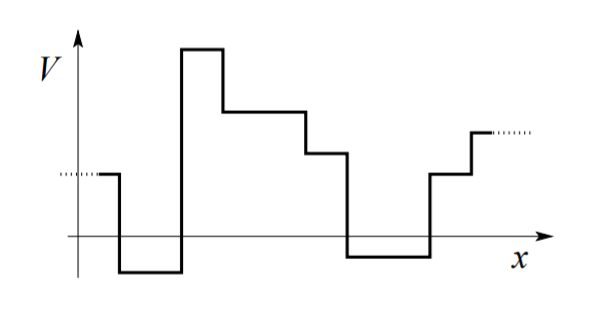
\includegraphics[scale=1]{3_1.PNG}
    \captionsetup{font={Large}}
    \caption{Piecewise constant potential.}
    \label{fig:3_1}
\end{figure}
As special cases we then examine different potentials with exemplary character, in particular bound states in pot (Figure 3.2 (a)), the tunneling effect through a potential barrier (Figure 3.2 (b)), different scattering problems that lead to resonances ( Fig. 3.2 (c) and (d)), the $\delta$-function potential (Fig. 3.2 (e)), periodic potentials leading to energy bands (Fig. 3.2 (f)), or disordered potentials representing the wave function locate (Figure 3.2 (g)).\\\\
\begin{figure}[ht]
    \centering
    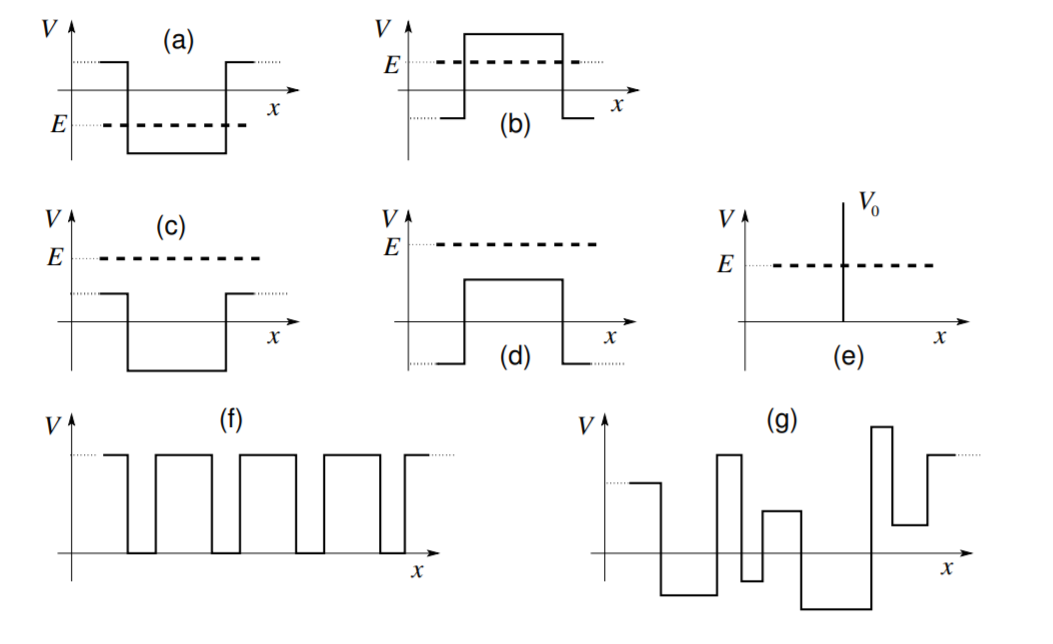
\includegraphics[scale=1]{3_2.PNG}
    \captionsetup{font={Large}}
    \caption{(a) Bonded states in pot, (b) tunneling effect through potential barrier, (b), (c), (d) and (e) scattering problems and resonances, (e) δpotential, (f) periodic potential, (g) random potential.}
    \label{fig:3_2}
\end{figure}
Then we consider some exactly solvable cases, the harmonic oscillator, see Fig. 3.3 (a), the Morse potential, see Fig. 3.3 (b), the $cosh^{-2} x$ potential, see Fig. 3.3 (c) , and the constant force field, cf. Fig. 3.3 (d). In all cases, the Hamiltonian has the form $H = p^2 / 2m + V (x)$, where the potential $V (x)$ takes the form described.
%图 3.3
\begin{figure}[ht]
    \centering
    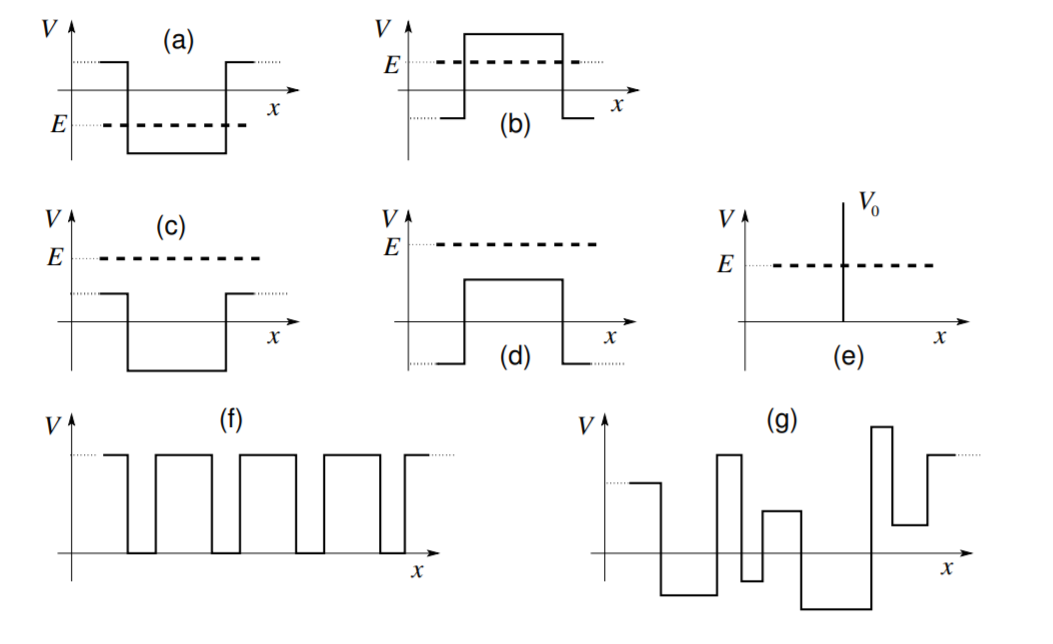
\includegraphics[scale=1]{3_2.PNG}
    \captionsetup{font={Large}}
    \caption{Exactly solvable problems: (a) harmonic potential, (b) the Morse potential that approximates a surface potential, (c) the Cosekans hyperbolic potential (the corresponding eigenvalue problem occurs in different situations), (d) the constant Force field, eg, an electron in the electric field.}
    \label{fig:3_3}
\end{figure}

%Page79
\section{Transfermatrix formalism}
Consider the potential level outlined in Figure 3.4. We are interested in stationary states Ψ which satisfy the time independent equation $H\Psi = E\psi$. The generic solutions to this eigenvalue problem with stuck constant $V$ are $exp \pm ikx)$ if $E> V$ and $exp (\pm αx)$ for $E <V$. Accordingly, we define the wave functions
%图 3.4
\begin{figure}[ht]
    \centering
    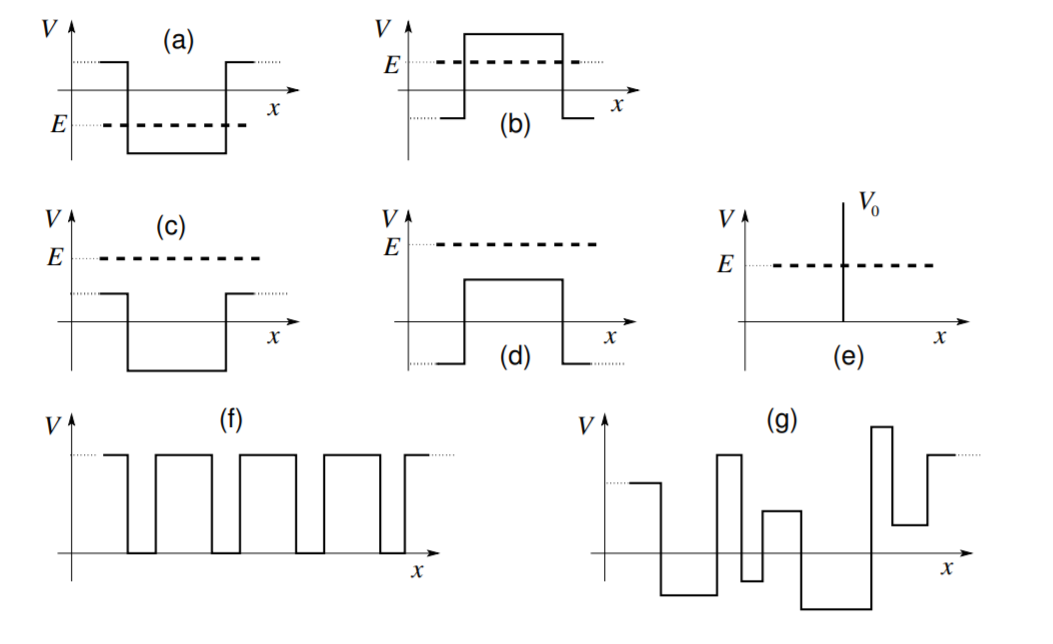
\includegraphics[scale=1]{3_2.PNG}
    \captionsetup{font={Large}}
    \caption{Potential level as element in the transfer matrix
    Formalism.}
    \label{fig:3_4}
\end{figure}
%公式 3.1
\begin{equation}
    \Psi_l=ae^{ikx}+b^{-ikx},\quad \Psi_r=Ae^{-\alpha x}+Be^{\alpha x}
\end{equation}
with
%公式 3.2
\begin{equation}
    k=\sqrt{2mE}/\hbar,\quad \alpha=\sqrt{2m(E_b-E)}/\hbar.
\end{equation}
Stationary states of H must be continuous in $x$ such that $\Psi_l (0) = \Psi_r (0)$ and $\Psi_l^{\prime} (0) = \Psi_r^{\prime} (0)$, where $\prime$ is the usual derivative $\partial x = d / dx$ denotes (otherwise ∂2xin H produces a $\delta$-function in $0$, if in Hamiltonian different (effective) masses $m_l \neq m_r$ the correct hermitian form must be used). The evaluation of the continuity condition connects the amplitudes,
%图 3.5
\begin{figure}[ht]
    \begin{minipage}{0.5\textwidth}
        \centering
        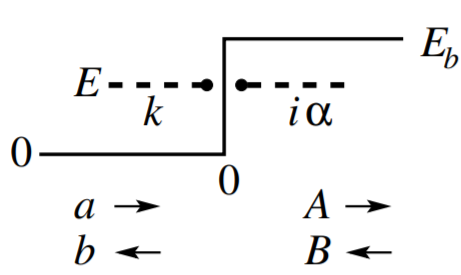
\includegraphics[scale=1]{3_5.PNG}
        \captionsetup{font={Large}}
        \caption{Potential step}
    \end{minipage}
    \begin{minipage}{0.5\textwidth}
        \begin{equation}
            \begin{aligned}
            \left(\begin{array}{cr}{a} 
            \\ {b}\end{array}\right) &=\frac{1}{2}\left(\begin{array}{cc}{1+\frac{i \alpha}{k}} & {1-\frac{i \alpha}{k}} 
            \\ {1-\frac{i \alpha}{k}} & {1+\frac{i \alpha}{k}}\end{array}\right)\left(\begin{array}{c}{A} 
            \\ {B}\end{array}\right) 
            \\ &=M\left(\begin{array}{cc}{A} 
            \\ {B}\end{array}\right), \quad \operatorname{det} M=\frac{i \alpha}{k} &
            \end{aligned}
            \end{equation}
            
            \begin{equation}
                \begin{aligned}
                \left(\begin{array}{cr}{A} 
                \\ {B}\end{array}\right) &=\frac{1}{2}\left(\begin{array}{cc}{1+\frac{k}{i \alpha}} & {1-\frac{k}{i \alpha}} 
                \\ {1-\frac{k}{i \alpha}} & {1+\frac{k}{i \alpha}}\end{array}\right)
                \left(\begin{array}{c}{a} 
                \\ {b}\end{array}\right) 
                \\ &=M^{-1}\left(\begin{array}{cc}{a} 
                \\ {b}\end{array}\right), \quad \operatorname{det} M^{-1}=\frac{k}{i \alpha} &
                \end{aligned}
                \end{equation}
    \end{minipage}

\end{figure}
%公式 3.3
%公式 3.4
%Page80
Likewise, we obtain the transfer matrix (using the approach $Ψ_l = ae^{-αx} + be^{αx}$ and $Ψ_r = Ae^{ikx} + Be^{-ikx}$)for the inverse step
图 3
%公式 3.5
\begin{figure}[ht]
    \begin{minipage}{0.5\textwidth}
        \centering
        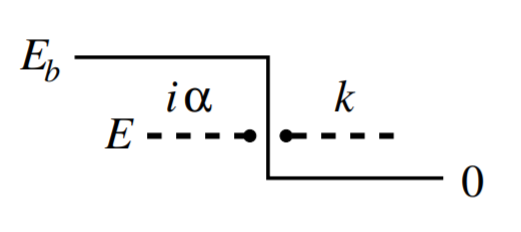
\includegraphics[scale=1]{3_5_1.PNG}
    \end{minipage}
    \begin{minipage}{0.5\textwidth}
        \begin{equation}
            \begin{aligned}
                M = &\frac{1}{2}\left(\begin{array}{cc}{1+\frac{k}{i \alpha}} & {1-\frac{k}{i\alpha}}\\{1-\frac{k}{i\alpha}}&{1+\frac{k}{i\alpha}}
                \end{array}\right),
                \\& \operatorname{det}M=\frac{k}{i\alpha},
            \end{aligned}
        \end{equation}
    \end{minipage}
\end{figure}
and further:\\
%公式 3.6
\begin{figure}[ht]
    \begin{minipage}{0.5\textwidth}
        \centering
        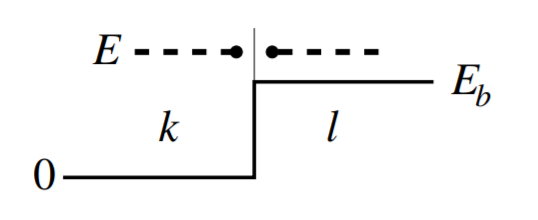
\includegraphics[scale=1]{3_5_2.PNG}
    \end{minipage}
    \begin{minipage}{0.5\textwidth}
        \begin{equation}
            \begin{aligned}
                M = &\frac{1}{2}\left(\begin{array}{cc}{1+\frac{l}{k}} & {1-\frac{l}{k}}\\{1-\frac{l}{k}}&{1+\frac{l}{k}}
                \end{array}\right),
                \\l =& \sqrt{2m(E-E_b)}/\hbar<k,
            \end{aligned}
        \end{equation}
    \end{minipage}
\end{figure}

%公式 3.7
\begin{figure}[ht]
    \begin{minipage}{0.5\textwidth}
        \centering
        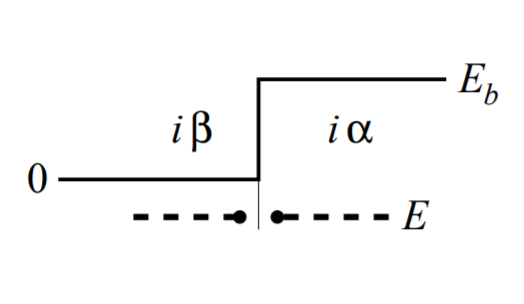
\includegraphics[scale=1]{3_5_3.PNG}
    \end{minipage}
    \begin{minipage}{0.5\textwidth}
        \begin{equation}
            \begin{aligned}
                M = &\frac{1}{2}\left(\begin{array}{cc}{1+\frac{k}{l}} & {1-\frac{k}{l}}\\{1-\frac{k}{l}}&{1+\frac{k}{l}}
                \end{array}\right),
                \\& \operatorname{det}M=\frac{k}{l},
            \end{aligned}
        \end{equation}
    \end{minipage}
\end{figure}

%公式 3.8
\begin{figure}[ht]
    \begin{minipage}{0.5\textwidth}
        \centering
        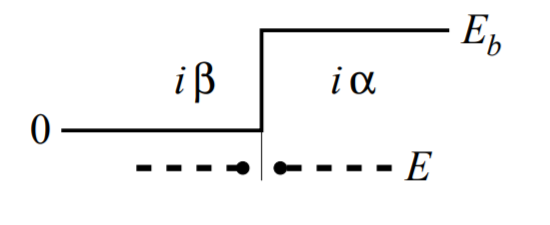
\includegraphics[scale=1]{3_5_4.PNG}
    \end{minipage}
    \begin{minipage}{0.5\textwidth}
        \begin{equation}
            \begin{aligned}
                M = &\frac{1}{2}\left(\begin{array}{cc}{1+\frac{\alpha}{\beta}} & {1-\frac{\alpha}{\beta}}\\{1-\frac{\alpha}{\beta}}&{1+\frac{\alpha}{\beta}}
                \end{array}\right),
                \\\beta =& \sqrt{2m(-E)}/\hbar<\alpha,
            \end{aligned}
        \end{equation}
    \end{minipage}
\end{figure}
%公式 3.9
\begin{figure}[ht]
    \begin{minipage}{0.5\textwidth}
        \centering
        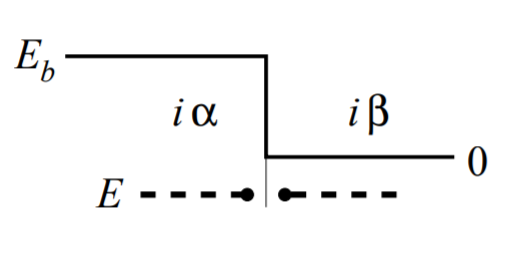
\includegraphics[scale=1]{3_5_5.PNG}
    \end{minipage}
    \begin{minipage}{0.5\textwidth}
        \begin{equation}
            \begin{aligned}
                M = &\frac{1}{2}\left(\begin{array}{cc}{1+\frac{\beta}{\alpha}} & {1-\frac{\beta}{\alpha}}\\{1-\frac{\beta}{\alpha}}&{1+\frac{\beta}{\alpha}}
                \end{array}\right),
                \\& \operatorname{det}M=\frac{\beta}{\alpha},
            \end{aligned}
        \end{equation}
    \end{minipage}
\end{figure}
In addition, we need matrices, which are the 'propagation' over and over again describe constant potentials. For positive energies take legal and left-hander the phases $exp (ikw)$ and $exp (-ikw)$, where w denotes the propagation distance; in the area of ​​forbidden propagation, the waves are damped, $\Psi^{\to}_r = e^{-αw}Ψ^{\to}_l$ for right-wing and $\Psi^{\leftarrow}_l = e^{-αw}Ψ^{\gets}_r$ for left-handers, where $r$ and $l$ are the right and left ends of the left Interval (see sketch) and the arrows $\to$ or $\gets$ specify the directions. Furthermore, right and left runners do not mix, which results in the transfer matrices.\\
%图
%公式 3.10
\begin{figure}[ht]
    \begin{minipage}{0.5\textwidth}
        \centering
        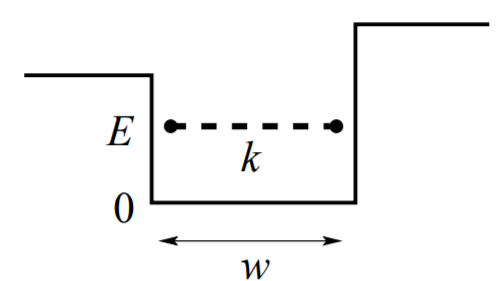
\includegraphics[scale=1]{3_5_6.PNG}
    \end{minipage}
    \begin{minipage}{0.5\textwidth}
        \begin{equation}
            \begin{aligned}
                \widetilde{M} = &\frac{1}{2}\left(\begin{array}{cc}{e^{-ikw}} & {0}\\{0}&{e^{ikw}}
                \end{array}\right),
                \\& \operatorname{det}\widetilde{M}=1,
            \end{aligned}
        \end{equation}
    \end{minipage}
\end{figure}

%公式 3.11
\begin{figure}[ht]
    \begin{minipage}{0.5\textwidth}
        \centering
        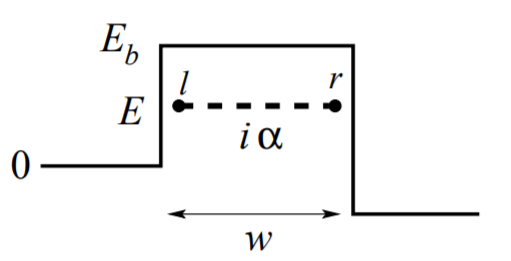
\includegraphics[scale=1]{3_5_7.PNG}
    \end{minipage}
    \begin{minipage}{0.5\textwidth}
        \begin{equation}
            \begin{aligned}
                \widetilde{M} = &\frac{1}{2}\left(\begin{array}{cc}{e^{\alpha w}} & {0}\\{0}&{e^{-\alpha w}}
                \end{array}\right),
                \\& \operatorname{det}\widetilde{M}=1,
            \end{aligned}
        \end{equation}
    \end{minipage}
\end{figure}
The whole problem with stuck wise constant potentials
%图 3.6
\begin{figure}[ht]
    \centering
    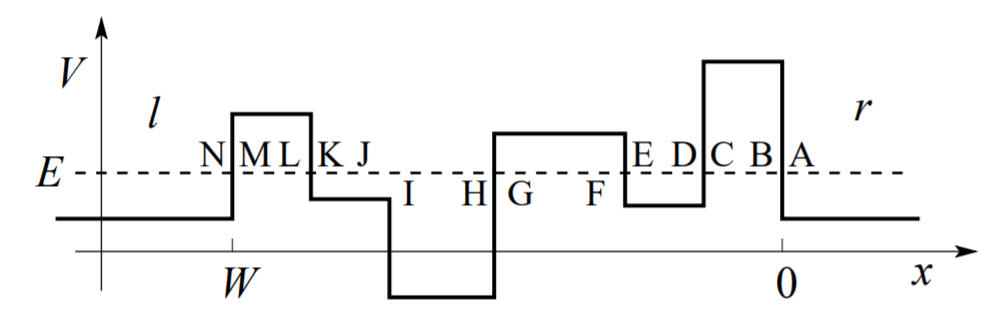
\includegraphics[scale=1]{3_6.PNG}
    \captionsetup{font={Large}}
    \caption{Piecewise constant potential with arbitrary shape.}
\end{figure}
is solved by a simple matrix multiplication; Let the wave function on the right side be given by
%公式 3.12
\begin{equation}
\Psi_r=\left(\begin{array}{cc}{A}\\{B}\end{array}\right),
\end{equation}
then the wave function $Ψ_l$ on the left side results as
%公式 3.13
\begin{equation}
    \begin{aligned}
        \Psi_l = \left(\begin{array}{cc}
            {a}\\{b}
        \end{array}\right)=&M_{NM}\widetilde{M}_{ML}M_{LK}\widetilde{M}_{KJ}M_{JI}\widetilde{M}_{IH}M_{HG}\\
        &\times \widetilde{M}_{GF}M_{FE}\widetilde{M}_{ED}M_{DC}\widetilde{M}_{CB}M_{BA}\left(\begin{array}{cc}
            {A}\\{B}
        \end{array}\right).
    \end{aligned}
\end{equation}

%Page82
Note that the wave functions $Ψ_l$ and $Ψ_r$ are given by
%3.14
\begin{equation}
    \begin{split}
        &\Psi_r = Ae^{ikx}+Be^{-ikx}\\
        &\Psi_l = ae^{ik(x-W)}+be^{-ik(x-W)},\quad (here, W<0)
    \end{split}
\end{equation}
since the matrices $M$ were always referenced to $x = 0$. Of course, the relevant $\alpha, \beta, k, l$ and propagation distances $w$ are always to be used. The above formalism is particularly suitable for numerical solutions (by computer). Since the complete information is always calculated, the solution of specific questions (with some coefficients A$, B, a, b = 0$) is often simpler by means of direct analysis instead of transfer matrix technique.

\section{Scatter Matrix}
An important quantity related to the transfer matrix $M$ is the scattering matrix $S$: Whilst the transfer matrix has the amplitudes $A, B,\cdots $ on the right side of the potential with the amplitudes $a, b,\cdots$ to the left of the potential, the scattering matrix connects the incident amplitudes (e.g., $a$ and $B$) with the falling out amplitudes (e.g., $A$ and $b$),
%公式 3.15
\begin{equation}
\begin{aligned} 
\Psi_{\mathrm{out}}=&\quad
    \left(\begin{array}{c}{b} \\ {A}\end{array}\right) &=\left(\begin{array}{cc}{r} & {t^{\prime}} \\ {t} & {r^{\prime}}\end{array}\right)\left(\begin{array}{c}{a} \\ {B}\end{array}\right)=S \Psi_{\mathrm{in}} ,
\\ & (\stackrel{b}{\leftarrow} \operatorname{Out} \stackrel{A}{\rightarrow})&=\left(\begin{array}{cc}{S_{L L}} & {S_{L R}} 
\\ {S_{R L}} & {S_{R R}}\end{array}\right)(\stackrel{a}{\rightarrow} \operatorname{In} \stackrel{B}{\leftarrow}) 
\end{aligned}
\end{equation}
The matrix elements $S_{LL} = r$ and $S_{LR} = t^{\prime}$ reflect and transmit left-incidence particles (amplitude $a$) to the left and right-incident particles (amplitude $B$) to the left and correspondingly to $S_{RL} = t$ and $S_{RR} = r^{\prime}$. The particle number preservation requires that $S$ be unitary, $S^{\dagger}S = \mathbb{I}$, which yields the following conditions for the coefficients (for $SS^{\dagger} = \mathbb{I}$ one shows that $r$ follows that $| t |$ and $| r | 2 = 1$, etc)
%公式 3.16
\begin{equation}
    \mid t\mid^2 + \mid r\mid^2 \,= \, 1 \,= \,\mid t^{\prime}\mid^2 + \mid r^{\prime}\mid^2,
\end{equation}
%公式 3.17
\begin{equation}
    r^{\prime *}t+t^{\prime *}r = 0,
\end{equation}
%公式 3.18
\begin{equation}
    t^* r^{\prime}+r^*t^{\prime}=0,
\end{equation}
%公式 3.19
\begin{equation}
    \quad \to r^{\prime}=-r^*t^{\prime}/t^*.
\end{equation}
The time-reversal invariance (T-invariance, when the magnetic field disappears $H = 0$) requires that with $\Psi, \Psi^*$ must be a solution,
%page 83
$\Psi^*_{in} = S\Psi^*_{out}$ from which we derive the condition
%公式 3.20
\begin{equation}
    \to t=t^{\prime}  
\end{equation}
(or $S = S^T$). Finally, for a symmetric scattering potential ($P$-invariant, $PSP = S$ with $P = \sigma_x$ the Pauli-matrix)
%公式 3.21
\begin{equation}
    \to r^{\prime}=r,\, t^{\prime}=t.
\end{equation}
Thus we find the scattering matrix in the form ($T$-invariant, $P$-invariant)
%公式 3.22
\begin{equation}
    S = \left(\begin{array}{cc}{r}&{t}\\{t}&{r}
    \end{array}\right),
\end{equation}
with $\mid r\mid ^2 + \mid t\mid^2=1$ and $t^*t=-r^*t$ and det $S=r/r^*=-t/t^*,\mid det S\mid = 1$.
%图 3.7
\begin{figure}[ht]
    \begin{minipage}{0.5\textwidth}
        \centering
        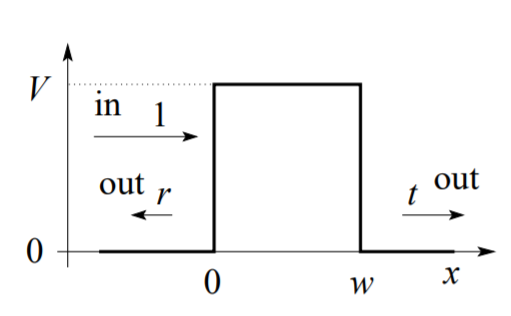
\includegraphics[scale=1]{3_7.PNG}
    \end{minipage}
    \begin{minipage}{0.5\textwidth}
        \captionsetup{font={Large}}
        \caption{The scattering matrix S transforms the incident amplitudes (here 1 from the left) into the outgoing amplitudes, here a transmitted t (to the right) and a reflected one (to the left).}
    \end{minipage}
\end{figure}
The amplitudes $r$ and $t$ are called reflection and transmission amplitudes. Consider a potential barrier between $x = 0 $and $x = w$ and a wave incident from the left with $a = 1$, e.g. Fig. 3.7; then a wave $t exp [ik (x - w)]$ is transmitted and a wave $r exp (-ikx)$ is reflected. (For a (parity) symmetric problem, with $\Psi(x)$ also $[P\Psi] (x ) = \Psi (-x)$ a solution, which describes a wave entering from the right and one recognizes immediately that $t+0 = t$ and $r_0 = r$ must be.) The phase $2φ$ of the reflection coefficient $r = | r |$ Within the quasi-classical approximation, $exp (i2φ)$ assumes the value $φ = \pi / 4$ for a linearly increasing potential; for an infinitely high potential, $φ = \pi / 2$, and the incident and reflected waves cancel out at the edges, $r = -1$ for the total reflection.\\
The form (3.22) can be diagonalized, 
%公式3.23
\begin{equation}
\begin{aligned} S_{D}=\left(\begin{array}{cc}{r+t} & {0} \\ {0} & {r-t}\end{array}\right)=\sqrt{\frac{t}{t^{*}}}\left(\begin{array}{cc}{e^{\pm i \varphi}} & {0} \\ {0} & {-e^{\mp i \varphi}}\end{array}\right) \\=\left(\begin{array}{cc}{e^{i(\delta \pm \varphi)}} & {0} \\ {0} & {-e^{i(\delta \mp \varphi)}}\end{array}\right) \end{aligned}
\end{equation}
with $t = |t|e^{i\delta},\delta$ is the phase of $t$ and $\varphi = arctan (| r | / | t |)$. (In a first step one finds the eigenvalues $​​r \pm t$. The unitarity relations $|t|^2+|r|^2=1, \text{ and } t^*r+r^*t=0$ imply that $| r \pm t |^2 = 1$. With the approach $t = | t | exp (i\delta), r = | r | exp (i\chi$ follows from $t^*r+r^*t = 0$, that $\chi = \delta \pm \pi / 2 + 2n\pi$. This yields eigenvalues ​​in the form $r + t = exp (i\delta) [(\pm i) | r | + | t |]$ and $r - t = exp (i\delta) [(\pm i) | r | - | t |]$. With $\varphi \equiv arctan (| r | / | t |)$ one finds the result $r + t = exp [i (\delta \pm \varphi)], r -t = - exp [i (\delta\mp\varphi)]$; the sign of $varphi$ results from the continuity of the solutions and changes with resonances ($r = 0$, note that then the phase $\chi = \delta \pm \pi / 2$ of $r$ also jumps by $\pi$), cf. the example of scattering at two $\delta$-potentials in Fig. 3.21)

\section{particles in the pot}
A potential well as shown in Fig. 3.8 binds states in a number determined by the potential depth V. The Heisenberg uncertainty principle gives us the energy scale of the problem: with Δx ≈ w Δp ~ ~ / w and we find the energy E0 = ~ 2 / 2mw2. The bound states in the potential well
%图 3.8
\begin{figure}[ht]
    \begin{minipage}{0.5\textwidth}
        \centering
        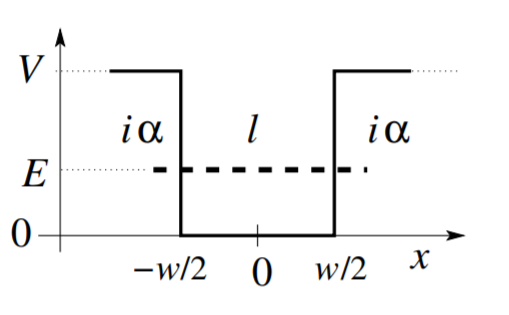
\includegraphics[scale=1]{3_8.PNG}
    \end{minipage}
    \begin{minipage}{0.5\textwidth}
        \captionsetup{font={Large}}
        \caption{Potential pot of width $w$ and depth $v$.}
    \end{minipage}
\end{figure}
can be found with the help of transfer matrix formalism. We construct the transfer matrix from the corresponding three elements,
%公式
$$
\begin{aligned}\left(\begin{array}{l}{a} \\ {b}\end{array}\right) &=\frac{1}{4}\left(\begin{array}{cc}{1+\frac{1}{i \kappa}} & {1-\frac{1}{i \kappa}} \\ {1-\frac{1}{i \kappa}} & {1+\frac{1}{i \kappa}}\end{array}\right)\left(\begin{array}{cc}{e^{-i l w}} & {0} \\ {0} & {e^{i l w}}\end{array}\right)\left(\begin{array}{cc}{1+i \kappa} & {1-i \kappa} \\ {1-i \kappa} & {1+i \kappa}\end{array}\right)\left(\begin{array}{c}{A} \\ {B}\end{array}\right) \\ &=M\left(\begin{array}{c}{A} \\ {B}\end{array}\right) \end{aligned}
$$
where $\kappa ≡ \alpha / l, \alpha = \sqrt{2m(V-E)}/\hbar, l=\sqrt{2mE}/\hbar$. With some trigonometry we find the transfer matrix
%公式 3.24
\begin{equation}
M=\left(\begin{array}{cc}{\cos l w-\sinh y \sin l w} & {-\cosh y \sin l w} \\ {\cosh y \sin l w} & {\cos l w+\sinh y \sin l w}\end{array}\right)
\end{equation}
with $y = - \operatorname{ln} \kappa$ and
%公式 3.25
\begin{equation}
    \sinh y=\frac{1}{2}\left(\frac{1}{\kappa}-\kappa\right), \quad \cosh y=\frac{1}{2}\left(\frac{1}{\kappa}+\kappa\right)
    \end{equation}
%Page85
We find the bound states by asking for normability. Accordingly, no exponentially growing components can occur, which is why the amplitudes a and B must disappear (no 'einfallende' particles),
%公式 3.26
\begin{equation}
\left(\begin{array}{l}{a} \\ {b}\end{array}\right)=\left(\begin{array}{l}{0} \\ {b}\end{array}\right),\left(\begin{array}{c}{A} \\ {B}\end{array}\right)=\left(\begin{array}{c}{A} \\ {0}\end{array}\right)
\end{equation}
This constraint forces the disappearance of the matrix element $M_{11}$ and we get the condition
%公式 3.27
\begin{equation}
    \cos l w=\sinh y \sin l w
    \end{equation}
which can be rewritten as$ cot x = [cot (x / 2) - tan (x / 2)] / 2$ and the relation (3.25)
%公式 3.28
\begin{equation}
    2 \cot l w=\cot (l w / 2)-\tan (l w / 2)=1 / \kappa-\kappa
    \end{equation}
With $cot x = 1 / tan x$ we ​​obtain the simpler transcendental equations
%公式 3.29
\begin{equation}
    \cot \frac{l w}{2}=-\kappa \quad \text { and } \quad \tan \frac{l w}{2}=\kappa
    \end{equation}
which can be solved graphically. For this we define new coordinates $\xi = lw / 2$ and $\eta = \alpha w / 2$ and find the relations
%公式 3.30
\begin{equation}
    \xi \cot \xi=-\eta, \quad \xi \tan \xi=\eta
    \end{equation}
The parameters $\xi = w\sqrt{2mE}/2\hbar$ and $\eta = w\sqrt{2m(V-E)}/2\hbar$ are linked via energy $E$ and potential $V$ and we get the second relation
%公式 3.31
\begin{equation}
    \xi^{2}+\eta^{2}=\frac{m w^{2} V}{2 \hbar^{2}} \overset{E_{0}=\hbar^{2} /2m w^{2}}{=} \frac{V}{4 E_{0}}
    \end{equation}
Figure 3.9 (a) illustrates the graphical solution to the problem. The solutions with even and odd numbers of nodes result alternately from the two transcendental equations; the energies result from the values ​​of $\xi$ via
%公式 3:32
\begin{equation}
    E=\frac{\hbar^{2} l^{2}}{2 m}=4 E_{0} \xi^{2}
\end{equation}
with the energy scale $E_0 = \hbar^2 / 2mw^2$; the associated eigenvalues ​​/ functions are shown in Figure 3.9 (b) and (c). An increase of $\xi$ by $\pi / 2$ gives another bound state if $\xi$ remains below the radius $\sqrt{V} / 4E_0$ of the circle (3.31). This immediately results in the maximum number of bound states nbound = $n_{bound}=\lfloor 2\xi/\pi\rfloor+1=\lfloor\sqrt{V/E_0}/\pi\rfloor+1$.
%page86
%图 3.9
\begin{figure}[ht]
        \centering
        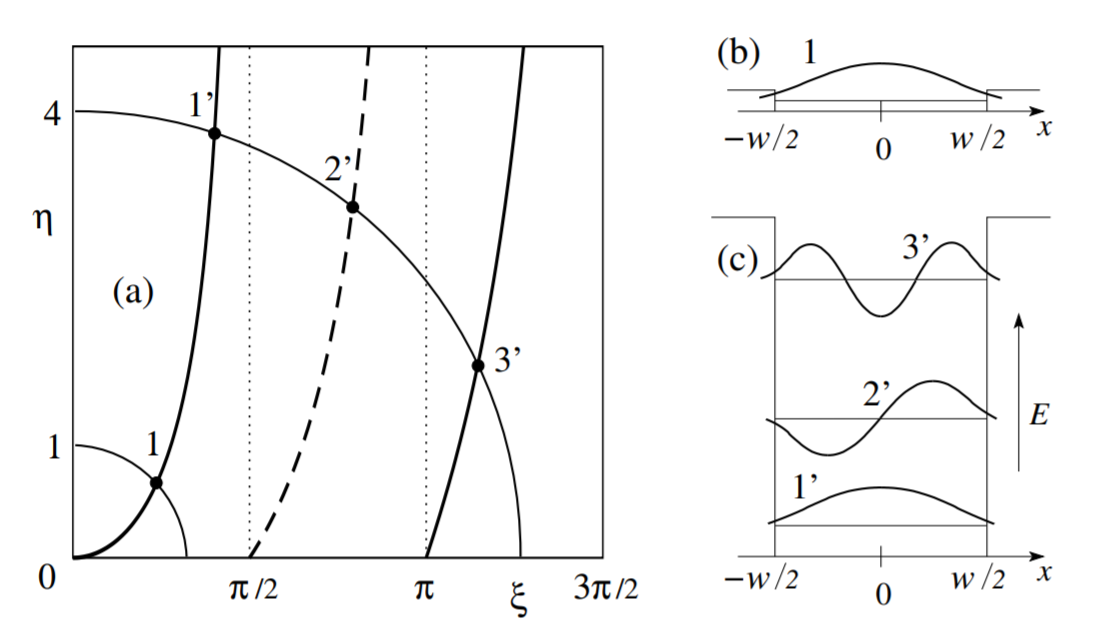
\includegraphics[scale=1]{3_9.PNG}
        \captionsetup{font={Large}}
        \caption{Energy eigenvalues and eigenfunctions for potential pots of depth $V = 4E_0$ and $V = 64E_0$. (a) Graphical solution of the transcendental equation with $\xi$ tan $\xi$ (straight solutions, solid lines) and $\xi$ cot $\xi$ (odd solutions, dashed lines). (b) Solution for the shallow pot with $V = 4E_0$, (c) Solutions for the deep pot with $V = 64E_0$.}
\end{figure}
\subsection{Parity}
For $V\to\infty$ results in wave functions of the form $\propto \operatorname{sin} (n\pi x / w)$ and $\propto \operatorname{cos} (n\pi x / w)$, cf. Section 1.6.2; these are odd and even in $x$. This symmetry for the wave functions also holds for potential heads of finite depth, that is, $V <\infty$; it is a consequence of the symmetry $x\longleftrightarrow -x$ of the Hamiltonian. We define the (symmetry) operator $P$, the parity operator
%公式 3:33
\begin{equation}
    (P \Psi)(x)=\Psi(-x), \quad\langle x|P| \Psi\rangle=\langle- x | \Psi\rangle
    \end{equation}
The Hamiltonian $H$ commutes with $P$, that is, $H$ is invariant under the exchange $x \longleftrightarrow -x$ since we chose $V (x)$ symmetrically, $V (x) = V (-x)$. In particular, the kinetic term is invariant under $x \longleftrightarrow -x: \partial_x^2\to (-\partial_x)^2=\partial_x^2$, and it is explicit that $\langle | HP | \Psi\rangle = \langle x | P H | \Psi\rangle$ for all $\Psi$ and all $x$,

%Page 87
%公式 3:34
\begin{equation}
\begin{aligned}\langle x|H P| \Psi\rangle &=\left[-\left(\hbar^{2} / 2 m\right) \partial_{x}^{2}+V(x)\right]\langle x|P| \Psi\rangle \\ &=\left[-\left(\hbar^{2} / 2 m\right) \partial_{x}^{2}+V(x)\right]\langle- x | \Psi\rangle \\ &=\left[-\left(\hbar^{2} / 2 m\right) \partial_{x}^{2}+V(-x)\right]\langle- x | \Psi\rangle \\
&=\langle- x|H| \Psi\rangle=\langle x|P H| \Psi\rangle
\end{aligned}
\end{equation}
$P$ is an involution, $P_2 = \mathbb{I}$, resulting in eigenvalues $\pm 1$. Since $H$ and $P$ commute, cf. the discussion on page 64, we can simultaneously diagonalize $H$ and $P$, that is, we can choose eigenvectors to $H$, which are at the same time eigenvectors to $P$ and thus either even or odd in $x$. Since $H$ has no other symmetry, dimEigEn = $1$ and our eigenfunctions to $H$ are automatically even or odd: the solutions to $\xi tan \xi= \eta$ are even (it obviously always exists at least one such solution) while the solutions to $\xi cot\xi = -\eta$ are odd. For $V <\pi^2E_0$ there is only one bound state. In special cases (or, more generally, if there is an additional symmetry), Dim $Eig_{E_n}> 1$, for example, could be a symmetric double-well potential with an infinitely high partition. Let the potential $V (x) = V (-x)$ be symmetric, then with $\phi n (x)$ we also get $\phi n (-x)$ as a solution. If dim $Eig_{E_n} = 1$ then $\phi n (-x) = (+ \text{ or } -) \phi n (x)$ and we find (anti-) symmetrical eigenfunctions. If dim$Eig_{E_n} ≥ 2$ then the linear combinations $\varphi_{g, u} = [\varphi_n (x) \pm \varphi_n (-x)] / \sqrt{2}$ define even or odd eigenfunctions in $Eig_{E_n}$.
In summary, let $H$ be symmetric with interchange $x \longleftrightarrow -x, [H, P] = 0, P$ is the parity operator, $P^2 = \mathbb{I}$. Let $\Psi$ be a solution to $H\Psi = E\Psi$, then also $\Phi\equiv P\Psi$ solution of the eigenvalue problem with the same energy, $H\Phi = HP\Psi = P H\Psi = P E\Psi = E\Phi$. It is either $\langle\Psi,\Phi\rangle = 0, \Phi ⊥ \Psi$, and $\Psi, \Phi $span at least one two-dimensional eigenspace ($\to$ (anti -) - symmetrize the wavefunctions) or $\Phi = \alpha\Psi=P\Psi\to P\Psi=\pm\Psi$ and $\Psi$ either even or odd. You can always find states that diagonalize both $H$ and $P$.
\section{Tunnel effect}
The tunnel effect describes the 'propagation' of a particle through an energetically forbidden zone, cf. Fig. 3.10, a pure quantum effect that is classically forbidden. Again, the tunneling effect can be described with the transfer matrix formalism; with $\kappa = k / \alpha$ we compose the transfer matrix $M$ from three elements and find it
%图 3.10
\begin{figure}[ht]
    \begin{minipage}{0.5\textwidth}
        \centering
        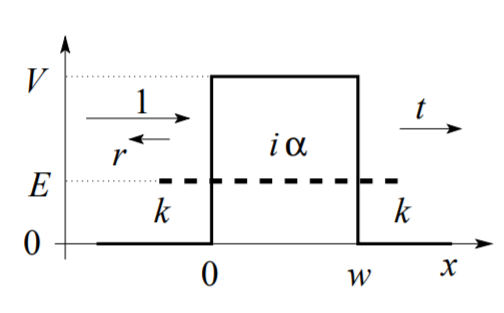
\includegraphics[scale=1]{3_10.PNG}
    \end{minipage}
    \begin{minipage}{0.5\textwidth}
        \captionsetup{font={Large}}
        \caption{Tunnel effect: Particles can penetrate a potential barrier. $t$ and $r$ are transmission and reflection coefficients and we define $\kappa = k / \alpha$.}
    \end{minipage}
\end{figure}
%公式 3:35
\begin{equation}
    \begin{split}
    \left(\begin{array}{l}{a} \\ {b}\end{array}\right)&=\frac{1}{4}\left(\begin{array}{cc}{1-\frac{1}{i \kappa}} & {1+\frac{1}{i \kappa}} \\ {1+\frac{1}{i \kappa}} & {1-\frac{1}{i \kappa}}\end{array}\right)\left(\begin{array}{cc}{e^{\alpha w}} & {0} \\ {0} & {e^{-\alpha w}}\end{array}\right)\left(\begin{array}{cc}{1-i \kappa} & {1+i \kappa} \\ {1+i \kappa} & {1-i \kappa}\end{array}\right)\left(\begin{array}{c}{A} \\ {B}\end{array}\right)\\
    &=M\left(\begin{array}{c}
        {A}\\{B}
    \end{array}\right)\\
    \end{split}
\end{equation}
%公式 3:36
\begin{equation}
M=\left(\begin{array}{cc}{\cosh \alpha w+i \sinh y \sinh \alpha w} & {i \cosh y \sinh \alpha w} \\ {-i \cosh y \sinh \alpha w} & {\cosh \alpha w-i \sinh y \sinh \alpha w}\end{array}\right)
\end{equation}
with $y = - \operatorname{ln} \kappa$ and
%公式 3:37
\begin{equation}
\sinh y=\frac{1}{2}\left(\frac{1}{\kappa}-\kappa\right), \quad \cosh y=\frac{1}{2}\left(\frac{1}{\kappa}+\kappa\right)
\end{equation}
The transfer matrices (3.36) and (3.24) are $\alpha$ equivalent under the interchange $l\longleftrightarrow i\alpha$. The tunnel configuration can also be understood as a scattering configuration, with incident and reflected (backscatter) amplitude $a = l$ and $b = r$, as well as a transmitted (previously scattered) amplitude $t$.
%公式 3:38
\begin{equation}
\left(\begin{array}{l}{a} \\ {b}\end{array}\right)=\left(\begin{array}{l}{1} \\ {r}\end{array}\right), \quad\left(\begin{array}{l}{A} \\ {B}\end{array}\right)=\left(\begin{array}{l}{t} \\ {0}\end{array}\right)
\end{equation}
The combination with (3.36) leads us to the transfer matrix in the form
%公式 3:39
\begin{equation}
M=\left(\begin{array}{cc}{\frac{1}{t}} & {\frac{r^{*}}{t^{*}}} \\ {\frac{r}{t}} & {\frac{1}{t^{*}}}\end{array}\right)
\end{equation}
with the properties (by comparison with (3.36))
%公式 3:40
\begin{equation}
\begin{aligned} \frac{r^{*}}{t^{*}} &=-\frac{r}{t}, \quad|r|^{2}+|t|^{2}=1 \\ \operatorname{det} M &=\frac{1}{|t|^{2}}-\frac{|r|^{2}}{|t|^{2}}=1 \\ M^{-1} &=\left(\begin{array}{cc}{\frac{1}{t^{*}}} & {-\frac{r^{*}}{t^{*}}} \\ {-\frac{r}{t}} & {\frac{1}{t}}\end{array}\right)=\left(\begin{array}{cc}{\frac{1}{t^{*}}} & {\frac{r}{t}} \\ {\frac{r^{*}}{t^{*}}} & {\frac{1}{t}}\end{array}\right)=M^{*} \end{aligned}
\end{equation}
For the calculation of $M^{-1}$ we have the usual relation
%公式 3:41
\begin{equation}
A=\left(\begin{array}{ll}{a} & {b} \\ {c} & {d}\end{array}\right) \quad \Leftrightarrow \quad A^{-1}=\frac{1}{\operatorname{det} A}\left(\begin{array}{cc}{d} & {-b} \\ {-c} & {a}\end{array}\right)
\end{equation}
used. The transmission $(t)$ and reflection $(r)$ coefficients defined here are identical to those in the scattering matrix,
%公式 3:42
\begin{equation}
S=\left(\begin{array}{ll}{r} & {t} \\ {t} & {r}\end{array}\right)
\end{equation}
whereas the scattering matrix S connects the amplitudes $(a\quad B)$ and $(b\quad A)$, the transfer matrix $M$ transposes the amplitudes $(A\quad B)$ into $(a \quad b)$. Although all particles are classically reflected (note that $E <V$) can quantum mechanically penetrate particles through the forbidden region and propagate further for $x> w$: this is the tunneling effect. The probability for the tunneling process is given by
%公式 3:43
\begin{equation}
    |t|^{2}=\frac{1}{1+\cosh ^{2} y \sinh ^{2} \alpha w}\overset{{\left(\frac{1}{\kappa}+\kappa\right)^{2}}=\frac{V^{2}}{2}}{=} \frac{1}{1+\frac{V^{2} \sinh ^{2} \alpha w}{4 E(V-E)}}
    \end{equation}
We used the relations $cosh^2 \alpha w - sinh^2 \alpha w = 1$ and $cosh^2 \alpha w + sinh^2 y sinh^2 \alpha w = 1 + cosh^2 y sinh^2 \alpha w$. The tunnel amplitude is given too
%公式 3:44
\begin{equation}
    t=\frac{2 i k \alpha}{2 i k \alpha \cosh \alpha w-\left(\alpha^{2}-k^{2}\right) \sinh \alpha w}
    \end{equation}
With $\alpha w = w\sqrt{2m (V - E)} / \hbar = \sqrt{ (V - E)} / E_0$ and $E_0, E\ll V$ we obtain
%公式 3:45
\begin{equation}
    |t|^{2} \approx \frac{16 E}{V} e^{-2 \sqrt{V / E_{0}}}, \quad t \approx-4 i \sqrt{\frac{E}{V}} e^{-\sqrt{V / E_{0}}}
    \end{equation}
or
%公式 3:46
\begin{equation}
    |t|^{2} \approx \frac{16 E}{V} e^{-2 w \sqrt{2 m V} / \hbar}, \quad t \approx-4 i \sqrt{\frac{E}{V}} e^{-w \sqrt{2 m V} / \hbar}
    \end{equation}
The tunneling probability is exponentially small in the distance w and in the forbidden momentum $\propto \sqrt{V}: \sqrt{(V - E) / E_0} = \alpha w = (\text{ forbidden pulse }/\hbar) · \text{ path } = ΔpΔx / \hbar$. Thus, the Heisenberg uncertainty principle (HUP) is ultimately responsible for the tunneling process: A particle can 'survive' a distance $Δx ~ \hbar / Δp$ in the forbidden regime. The exponent $\alpha w = \int p dx / \hbar$ measures how strongly prohibited the process is.\\\\
It is interesting to plot the trajectories of the reflection and transmission amplitudes $r$ and $t$ in the complex plane as a function of the energy E of the incident particle, see Fig. 3.11 and these with the results in Fig. 3.21 for the double barrier in section 3.7. 2 compare.
%图 3.11
\begin{figure}[ht]
    \centering
    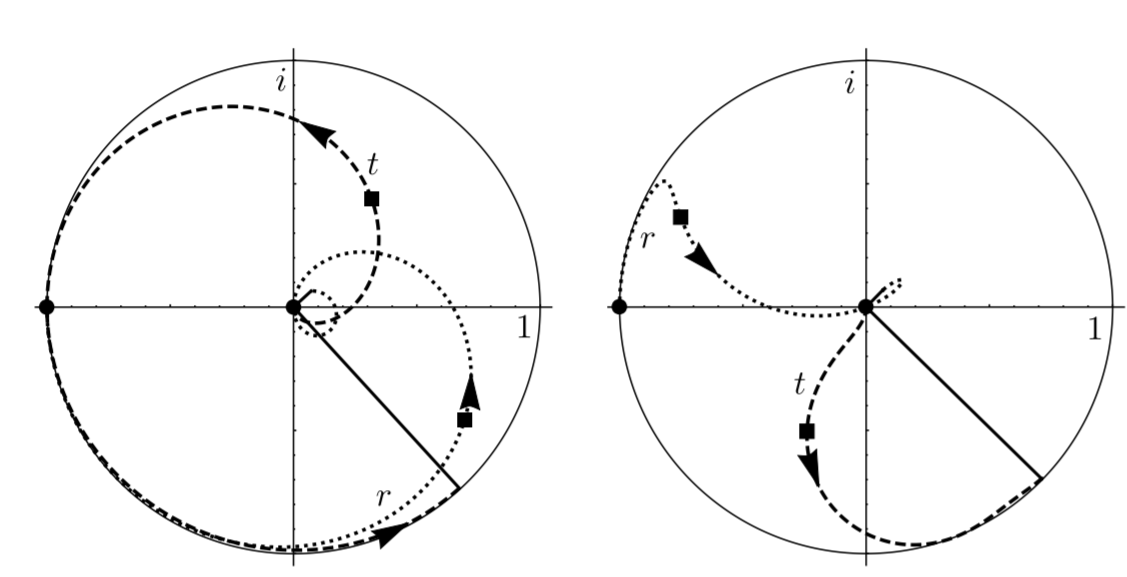
\includegraphics[scale=1]{3_11.PNG}
    \captionsetup{font={Large}}
    \caption{Trajectories of the reflection and transmission amplitudes $r$ (dotted) and $t$ (dashed) in the complex plane as a function of the energy $E$ of the incident particle ($E$ = curve parameter). The starting points at$ E = 0 (r = -1, t = 0)$ are marked by bold points $\bullet$. The marker $\blacksquare$ denotes the energy $E = V$ where the particle first hits the barrier can fly over. The vectors for $r$ and $t$ are orthogonal (according to $r^*t+t^*r=0$ for a symmetric potential). Left: $r$ and $t$ as defined in (3.38); the reflection coefficient $r$ follows the unit circle and falls through the center when $t = -1$ (first resonance); the transmission $t$ swings up to the unit circle and touches this in the resonances with energies $E> V$. Right: renormalized coefficients $r \to exp (-ikw) r$ and $t \to exp (-ikw) t$ reduced by the trivial propagation phase $kw$. The transmission $t$ approaches the asymptotic value 1
    by oscillating closer and closer to the unit circle.}
\end{figure}
The tunnel effect has multiple technical applications. On the one hand, these are 'everyday' effects such as the penetration of electrons (current) through oxide layers in semiconductors (electronics, transistors, see the work of Tsui \& Esaki, Appl. Phys. Lett., 22, 562 (1973), Sollner et al., Appl. Phys., Lett., 43, 588 (1983), Ricco \& Azbel, Phys., Rev. B, 29, 1970 (1984))., On the other hand, the effect has interesting applications such as the tunneling microscope (Binnig and Rohrer, Phys., Rev. Lett., 50, 120 (1983)), outlined in Figure 3.12.

%Page 91
%图 3.12
\begin{figure}[ht]
    \centering
    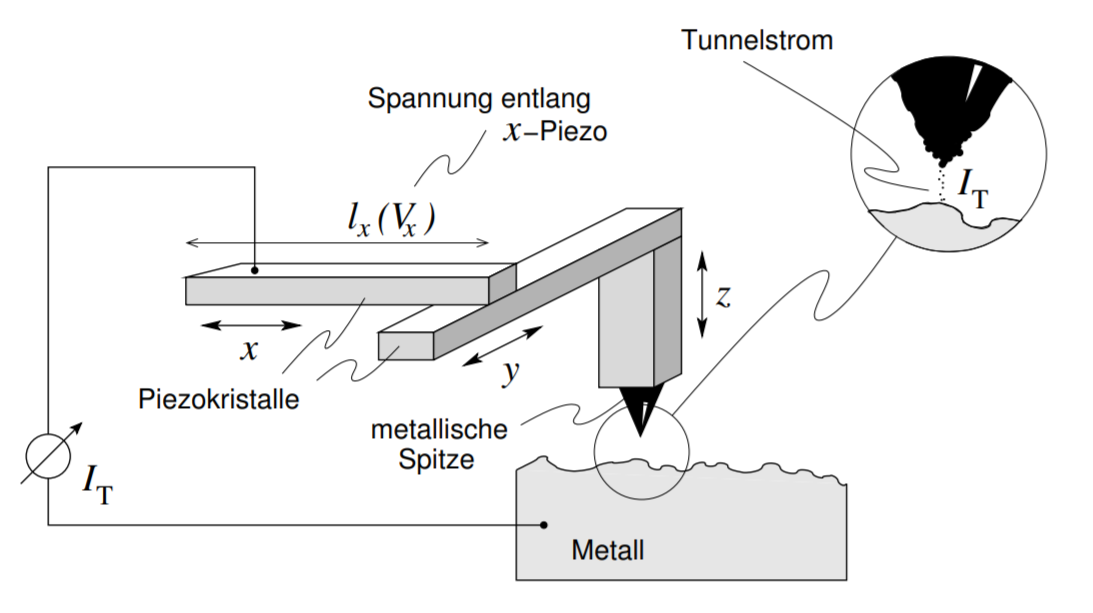
\includegraphics[scale=1]{3_12.PNG}
    \captionsetup{font={Large}}
    \caption{Tunneling microscope (Binnig \& Rohrer, IBM): The tunneling current IT flows from the metal tip of the microscope to the surface under investigation. The current $I_T$ depends sensitively (exponentially) on the distance tip-to-surface and can thus be used as control parameters: The current $I_T$ is transformed into a voltage $V_z (x, y)$ which manipulates the piezocrystal along $z$, so $I_T$ stays constant. The crystals along the $x, y$ plane serve to shift the tip ('scanning'). The potential relief $V_z (x, y)$ then serves as the elevation map of the surface.}
\end{figure}
\section{$\delta$-potential}
The solution for the $\delta$-potential, see Fig. 3.13, involves a special transfer matrix which is also useful in other situations, e.g. for the solution of the Kronig-Penney model or for the problem of the double barrier. To solve is the eigenvalue problem with the Hamiltonian
%公式 3:47
\begin{equation}
    H=-\frac{\hbar^{2}}{2 m} \partial_{x}^{2}+V_{0} \delta(x)
    \end{equation}
where the $\delta$-function forces special boundary conditions at 0. Note the units of [$V$] = energy, whereas that of [$V_0$] = energy · length. To get the boundary conditions at $\Psi_0 (x)$ at $x = 0$
integrate $H\Psi$ over the interval $[-\epsilon, \epsilon], \epsilon\to 0$, around 0,

%Page 92
%图 3.13
\begin{figure}[ht]
    \begin{minipage}{0.5\textwidth}
        \centering
        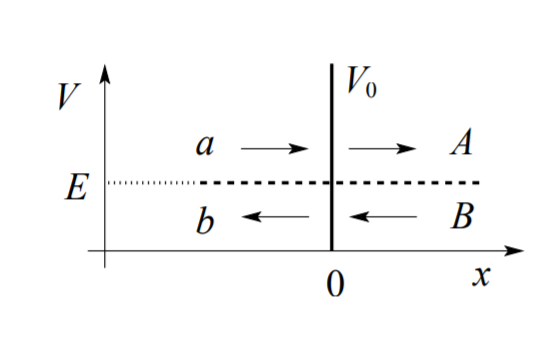
\includegraphics[scale=1]{3_13.PNG}
    \end{minipage}
    \begin{minipage}{0.5\textwidth}
        \captionsetup{font={Large}}
        \caption{Delta potential of the strength
        $V_0$.}
    \end{minipage}
\end{figure}
%公式 3:48
\begin{equation}
\begin{aligned} \int_{-\varepsilon}^{\varepsilon}\left[-\frac{\hbar^{2}}{2 m} \Psi^{\prime \prime}+V_{0} \delta(x) \Psi\right] d x &=\frac{\hbar^{2}}{2 m}\left(\Psi_{l}^{\prime}-\Psi_{r}^{\prime}\right)+V_{0} \Psi(0) \\ &=\int_{-\varepsilon}^{\varepsilon} E \Psi(x) d x=0 \end{aligned}
\end{equation}
With $\Psi_l (0) = \Psi_r(0)$ regular in 0 and (3.48) we get the equation system
%公式 3:49
\begin{equation}
\begin{aligned} a+b &=& A+B, & \quad k=\sqrt{2 m E} / \hbar \\ a(1-2 i v / k)-b(1+2 i v / k) &=&A-B, &\quad v=m V_{0} / \hbar^{2} \end{aligned}
\end{equation}
in matrix notation
%公式 3:50
\begin{equation}
\left(\begin{array}{l}{a} \\ {b}\end{array}\right)=\left(\begin{array}{cc}{1+i v / k} & {i v / k} \\ {-i v / k} & {1-i v / k}\end{array}\right)\left(\begin{array}{c}{A} \\ {B}\end{array}\right)
\end{equation}
the same result is obtained from (3.36) with $V · w = V0 = \text{ const. and }w \to 0,$
%公式 3:51
\begin{equation}
\begin{aligned} \alpha w &=\sqrt{2 m\left(w V_{0}-E w^{2}\right)} / \hbar \rightarrow 0 \\ \kappa &=\alpha / k=\sqrt{2 m\left(V_{0} / w-E\right)} / \hbar k \rightarrow \infty \end{aligned}
\end{equation}
In the following we consider both attractive and repulsive potentials:
\subsection{$V_0 <0$, bound state}
For bound states, the boundary condition applies
%公式 3:52
\begin{equation}
\left(\begin{array}{l}{a} \\ {b}\end{array}\right)=\left(\begin{array}{l}{0} \\ {b}\end{array}\right) \quad \text { and } \quad\left(\begin{array}{l}{A} \\ {B}\end{array}\right)=\left(\begin{array}{l}{A} \\ {0}\end{array}\right)
\end{equation}
%page 93
it produces the condition $1 + iv / k = 0$ which requires that $k \to i\alpha = i\sqrt{2m | E |} / \hbar$ be purely imaginary, which corresponds to a negative energy $E <0$. The energy eigenvalue results from
%公式 3:53
\begin{equation}
    1=-\frac{i v}{k}=\frac{m\left|V_{0}\right| \hbar}{\hbar^{2} \sqrt{2 m|E|}} \rightarrow E=-\frac{m V_{0}^{2}}{2 \hbar^{2}}
    \end{equation}
and we find for every $V_0 <0$ exactly one bound state (note that $dim = 1$), see Fig. 3.14.
%图 3.14
\begin{figure}[ht]
    \begin{minipage}{0.5\textwidth}
        \centering
        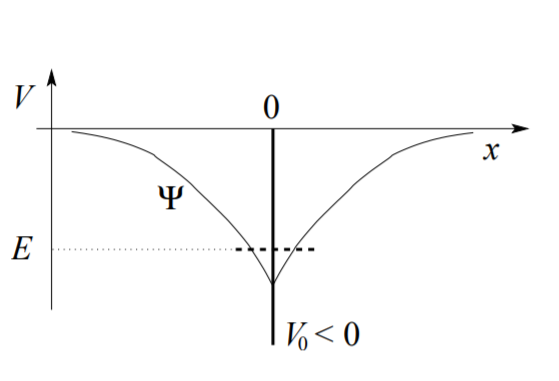
\includegraphics[scale=1]{3_14.PNG}
    \end{minipage}
    \begin{minipage}{0.5\textwidth}
        \captionsetup{font={Large}}
        \caption{The attractive $\delta$-potential in 1D binds exactly a condition. The kink in the wave function at $x = 0$ produces the compensating $\delta$-function after two derivatives. Compare also with the kink in the 1D Green's function to the operator $\mathcal{L}=\partial_x^2$}
    \end{minipage}
\end{figure}
\subsection{$V_0> 0$, scattering condition}
The transmission amplitude is
%公式 3:54
\begin{equation}
    t=\frac{1}{1+i v / k}, \quad|t|^{2}=\frac{1}{1+m V_{0}^{2} / 2 \hbar^{2} E}\overset{V_0 \text{ gross }}{\approx}\frac{2\hbar^2 E}{mV_0^2}
    \end{equation}
This result also follows from (3.43) with sinh αw ≈ αw and the substitutionV $-E \to V_0 / w-E \approx V_0 / w$. The relevant energy scale in the problem is given by $E = mV_0^2/2\hbar^2\sim V^2 / 4E_0$.
\section{Resonances}
We consider a pot potential as sketched in Fig. 3.15. The energy of the particle is positive this time, corresponding to a scattering configuration. Classically, we expect the particle to fly over the potential well - the quantum mechanical result is different.
Propagation again involves three subelements
%公式 3:55
\begin{equation}
\left(\begin{array}{l}{a} \\ {b}\end{array}\right)=\frac{1}{4}\left(\begin{array}{cc}{1+\frac{1}{\kappa}} & {1-\frac{1}{\kappa}} \\ {1-\frac{1}{\kappa}} & {1+\frac{1}{\kappa}}\end{array}\right)\left(\begin{array}{cc}{e^{-i l w}} & {0} \\ {0} & {e^{i l w}}\end{array}\right)\left(\begin{array}{cc}{1+\kappa} & {1-\kappa} \\ {1-\kappa} & {1+\kappa}\end{array}\right)\left(\begin{array}{l}{A} \\ {B}\end{array}\right)
\end{equation}
%Page94
%图 3.15
\begin{figure}[ht]
    \begin{minipage}{0.5\textwidth}
        \centering
        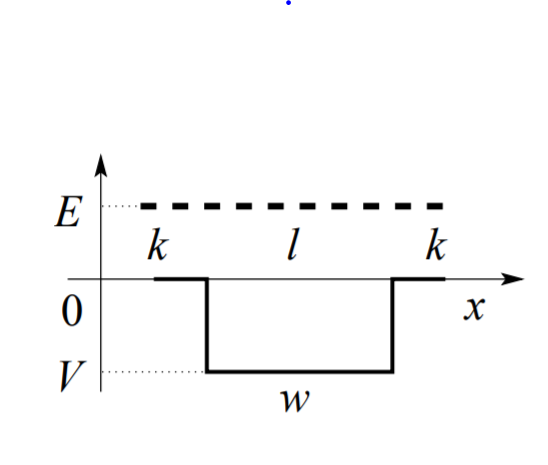
\includegraphics[scale=1]{3_15.PNG}
    \end{minipage}
    \begin{minipage}{0.5\textwidth}
        \captionsetup{font={Large}}
        \caption{Pot potential of depth V and width w which generates stray resonances. We define
        $k=\sqrt{2mE}/\hbar,l=\sqrt{2m(E-V)}/\hbar,\text{ and }\kappa=k/l.$}
    \end{minipage}
\end{figure}
and we find the transfer matrix for the scattering problem in the mold
%公式 3:56
\begin{equation}
M=\left(\begin{array}{cc}{\cos w l-i \cosh y \sin w l} & {-i \sinh y \sin w l} \\ {i \sinh y \sin w l} & {\cos w l+i \cosh y \sin w l}\end{array}\right)
\end{equation}
with $y = - ln \kappa$ and
%公式 3:57
\begin{equation}
    \sinh y=\frac{1}{2}\left(\frac{1}{\kappa}-\kappa\right), \quad \cosh y=\frac{1}{2}\left(\frac{1}{\kappa}+\kappa\right)
    \end{equation}
Printed by reflection and transmission amplitudes we can write
%公式 3:58
\begin{equation}
\left(\begin{array}{l}{a} \\ {b}\end{array}\right)=\left(\begin{array}{l}{1} \\ {r}\end{array}\right)=M\left(\begin{array}{l}{t} \\ {0}\end{array}\right)=M\left(\begin{array}{l}{A} \\ {B}\end{array}\right)
\end{equation}
with
%公式 3:59
\begin{equation}
\begin{aligned} M &=\left(\begin{array}{cc}{\frac{1}{t}} & {\frac{r^{*}}{t^{*}}} \\ {\frac{r}{t}} & {\frac{1}{t^{*}}}\end{array}\right) \\ t &=\frac{1}{\cos w l-i \cosh y \sin w l} \end{aligned}
\end{equation}
The transmission probability is
%公式 3.60
\begin{equation}
    |t|^{2}=\frac{1}{1+\left[\sin ^{2}(w l) V^{2}\right] / 4 E(E-V)}
    \end{equation}
and $| t |^2 <1$ in general. This means that quantum-mechanical particles can also be reflected at potential with energies $E> V (x)$, which would not be classically possible; Quantum mechanical and classical scattering processes are different. Perfect transmission occurs under the condition $| t |^2 = 1$; this is the case for $sin^ 2 wl = 0$. The condition $l = n\pi / w$,
then gives the associated energies
%公式 3.61
\begin{equation}
    E_{\mathrm{res}}=\frac{\hbar^{2} \pi^{2}}{2 m w^{2}} n^{2}+V=E_{0}(n \pi)^{2}+V
    \end{equation}
The number of bound states follows from the condition $E_0 (n\pi)^2 + V <0, n> \sqrt{| V | / E0 /} \pi$, and we find the minimum $n$ for a resonance,
%公式 3.62
\begin{equation}
    n_{\min }>\lceil\sqrt{|V| / E_{0}}\rceil= n_{\text {bound }}
    \end{equation}
A pretty application example is the resonant tunnel diode, cf. Fig. 3.16. The transmission amplitude has the form
%图 3.16
\begin{figure}[ht]
    \begin{minipage}{0.5\textwidth}
        \centering
        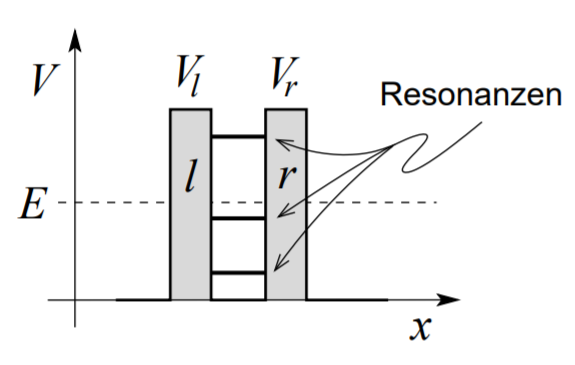
\includegraphics[scale=1]{3_16.PNG}
    \end{minipage}
    \begin{minipage}{0.5\textwidth}
        \captionsetup{font={Large}}
        \caption{Double barrier for the resonant tunnel diode.}
    \end{minipage}
\end{figure}
%公式 3.63
\begin{equation}
    t(E)=\frac{C_{0}}{C_{1} T_{l} T_{r}+C_{2} T_{l} / T_{r}+C_{3} T_{r} / T_{l}+C_{4} / T_{l} T_{r}}
    \end{equation}
with the transmission coefficients $T_l$ and $T_r$ for the left and right barrier. We choose $V_l$, $V_r$ large, $E$ small, so that $T_l, T_r \ll 1$. Thus, $(E) ≈ (C_0 / C_4) T_lT_r \ll 1$, unless $C_4 = 0$. If one chooses $E$ such that $C_4 (E) = 0$ vanishes, then $t (E) \approx CT_{min} / T_{max} \sim 1$ for $T_l = T_r$ (symmetric barriers). The resonant tunnel diode RTD is a useful device with negative differential resistance (NDR) in certain voltage ranges, cf. Fig. 3.17.
3.7 Analyticity
The analytic structure of the transmission coefficient $t (p)$ or $t (E)$ as a function of the momentum p or the energy E provides information about bound states and resonances. For this we set the functions $t (p)$ and $t (E)$ into the complex $p$ and $e$ plane. The relationship between the momentum $p = \sqrt{2mE}$ and the energy $E$ is given by
%公式 3.64
\begin{equation}
    E=\frac{p^{2}}{2 m}, \quad p=\sqrt{2 m E}
    \end{equation}
with the complex root defined via
%公式 3.65
\begin{equation}
    \sqrt{z}=\sqrt{|z|} e^{i \arg (z) / 2} \operatorname{mit} \arg z \in[0,2 \pi)
    \end{equation}
%图 3.17
\begin{figure}[ht]
        \centering
        \includegraphics[scale=1]{3_17.PNG}
        \captionsetup{font={Large}}
        \caption{Left: Double barrier of the resonant tunnel diode under voltage Vext. The transmission through the double barrier increases dramatically when electrons in the left conductor are resonant to a quasi-bound state within the double barrier. Right: I-V characteristic of a resonant tunnel barrier with resonance peaks. The negative differential resistance (NDR) is used technologically.}
\end{figure}
and is shown in Fig. 3.18. The physical plane is the first Riemann plane of $E$ with $\operatorname{Im} p> 0$.
%图 3.18
\begin{figure}[ht]
    \centering
    \includegraphics[scale=1]{3_18.PNG}
    \captionsetup{font={Large}}
    \caption{Complex $p$ plane and its mapping into the complex $E$ plane with two Riemann surfaces.}
\end{figure}
\subsection{Poles of $t$, Zeros $t^{-1} = 0$}
 Examination of the zeros of $t^{-1}$ or poles of $t$ for the pot potential gives the conditions
%公式 3.66
\begin{equation}
    2 i k l t^{-1}=2 i k l \cos l w+\left(k^{2}+l^{2}\right) \sin l w=0
    \end{equation}
Equation (3.66) is satisfied when
%公式 3.67
\begin{equation}
    2 \cot l w=\cot \frac{l w}{2}-\tan \frac{l w}{2}=\frac{i k}{l}-\frac{l}{i k}\\
    \cot \frac{l w}{2}=\frac{i k}{l} \text {  or  } \tan \frac{l w}{2}=-\frac{i k}{l}
    \end{equation}
The comparison with (3.29) shows that these conditions give just the bound states, where $ik$ just equals $-\alpha$ for a negative energy $E <0$,
%公式 3.68
\begin{equation}
\begin{aligned} i k &=\frac{i}{\hbar} \sqrt{2 m E} \stackrel{E<0}{=}-\alpha, \quad \alpha=\sqrt{2 m|E|} / \hbar \\ \Rightarrow \cot \frac{l w}{2} &=\frac{-\alpha}{l}, \quad \tan \frac{l w}{2}=\frac{\alpha}{l} \end{aligned}
    \end{equation}
Thus the poles of $t$ lie on the imaginary axis in $p$, $p \in i\mathbb{R}^+$ or on the negative semiaxis $E <0$. The poles of t lie in the first Riemann plane; they are physically relevant and describe bound states. 
\subsection{Resonances in $t, t \approx 1$}
 Next we investigate t (E) near a resonance, $wl ≈ n\pi$ and $E_n = \hbar^2\pi^2 n^2 / 2mw^2$,
%公式 3.69
\begin{equation}
    \frac{1}{t}=\cos w l\left[1-\frac{i}{2}\left(\frac{k}{l}+\frac{l}{k}\right) \tan w l\right] \approx \pm 1
    \end{equation}
It is $\operatorname{cos} wl \approx 1$ and we can develop the second factor in $E - E_n$ (use that tan $wl | E_n = 0$)
%公式 3.70
\begin{equation}
    1-\frac{i}{2} \frac{d}{d E}\left[\left(\frac{k}{l}+\frac{l}{k}\right) \tan w l\right]_{E_{n}}\left(E-E_{n}\right) \equiv 1-\frac{2 i}{\Gamma}\left(E-E_{n}\right)
    \end{equation}
%公式 3.71
\begin{equation}
    \operatorname{with} \quad \frac{4}{\Gamma}=\left.\left(\frac{k}{l}+\frac{l}{k}\right) \frac{d w l}{d E}\right|_{E_{n}}
    \end{equation}
Thus we obtain for $t(E)$ a rational function generated by a pole at $E = E_n - i\Gamma / 2$ in the lower complex half-plane,
%公式
$$
    t(E) \cong \frac{\pm i \Gamma / 2}{E-\left(E_{n}-i \Gamma / 2\right)}
$$
We obtain the pole at $E = E_n - i\Gamma / 2$ by analytically continuing $t (E)$ through the cut in $\mathbb{R}^+$ into the lower half-plane, so that this pole comes to rest in the second Riemann plane and is therefore unphysical.\\
This means that this pole does not correspond to a bound state. What we see on $E\in \mathbb{R}^+$ from this pole is a quasi-bound state, a resonance. The distance $\Gamma / 2$ from the axis $\mathbb{R}^+$ gives us the lifetime of the resonance / the quasi-bound state,
%公式 3.72
\begin{equation}
\begin{aligned} \Psi(x, t) \propto e^{-i E t / \hbar} &=e^{-i\left(E_{n}-i \Gamma / 2\right) t / \hbar} \\ &=e^{-i E_{n} t / \hbar} e^{-\Gamma t / 2 \hbar} \end{aligned}
\end{equation}
All of these properties (poles, resonances and phase shifts) are generally valid structures of the scattering matrix, which reappear in the scattering theory in dim = 3. Figure 3.19 summarizes these results.
We can write the amplitude $t (E)$ as a product of modulus and phase,
%公式 3.73
\begin{equation}
    t(E)=|t| e^{i \delta(E)}
    \end{equation}
the magnitude square $| t (E) |^2$ is described by a Lorentz curve, cf. Fig. 3.20 (a),
%公式 3.74
\begin{equation}
    |t|^{2} \cong \frac{\Gamma^{2} / 4}{\left(E-E_{n}\right)^{2}+\Gamma^{2} / 4}
    \end{equation}
and for the phase we get (modulo $\pi$)
%公式 3.75
\begin{equation}
    \delta(E)=\arctan \left[2\left(E-E_{n}\right) / \Gamma\right]
    \end{equation}
At each resonance, the phase $\delta (E)$ increases by $\pi$, cf. Fig. 3.20 (b). The value $\delta (E = 0)$ is related to the number of bound states, cf. Levinson's Theorem [e.g. in M. Sassoli de Bianchi, J. Math. Phys. 35, 2719 (1994)], $\delta (0) = (nbound - 1/2) \pi$ (case without $E = 0$ solution).
%图 3.19
\begin{figure}[ht]
    \centering
    \includegraphics[scale=1]{3_18.PNG}
    \captionsetup{font={Large}}
    \caption{Bound states produce a pole in $t (p), t (E)$ for $p \in i\mathbb{R}^+, E <0$ in the 1st Riemann plane. Resonances appear as poles in the transmission amplitude $t (E)$ for energies $E$ in the lower complex half-plane of the 2nd Riemann plane; they are unphysical.}
\end{figure}
%图 3.20
\begin{figure}[ht]
    \begin{minipage}{0.5\textwidth}
        \centering
        \includegraphics[scale=1]{3_20.PNG}
    \end{minipage}
    \begin{minipage}{0.5\textwidth}
        \captionsetup{font={Large}}
        \caption{(a) transmission probability $\mid t(t)\mid^2$ at a resonance $E_{n_2}> 0$; a bound state at $E_{n_1} <0$ corresponds to a $\delta$-function. (b) phase shift $\delta(E)$ in $t (E)$ via a resonance; the jump in $\pi$ is lubricated over the width $Gamma$ (= inverse lifetime of the resonance). A bound state corresponds to a sharp level.}
    \end{minipage}
\end{figure}
In Figure 3.21, the transmission amplitudes are $t = | t | exp (i\bar{\delta})$ and the associated reflection amplitude $r = | r | exp (i\bar{\chi})$ for the case of two repulsiver $\delta$ functions at a distance $w$. The phases $\bar{\delta} = \delta - kw \text{ and } \bar{\chi}=\chi-kw$ of the transmission and reflection amplitudes $t$ and $r$ involve the additional shift $-kw$; one finds this correction by using a single reference point instead of different reference points for the plane waves $\Psi_l$ and and $\Psi_r$, cf. (3.14).
%图 3.21
\begin{figure}[ht]
    \begin{minipage}{0.5\textwidth}
        \centering
        \includegraphics[scale=1]{3_21.PNG}
    \end{minipage}
    \begin{minipage}{0.5\textwidth}
        \captionsetup{font={Large}}
        \caption{Transmission ($t=\mid t\mid exp(i\bar{\delta})$) and reflection ($r=\mid r\mid exp(i\bar{\mathcal{X}})$) amplitudes for two repulsive $\delta$-functions at distance $w$. The plot starts at the energy $E = 0$ where $(t, r) = (0, -1)$ (black point) and runs through two resonances with $\mid t \mid = 1$. For $E\to\infty$, $t$ in turns approximates the value 1. The reflection amplitude r stands, according to $t^*r+r^*t=0$ perpendicular
        on $t$ (white dot). The phase $\mathcal{X}$
        jumps $\pm\pi$ at each resonance.}
    \end{minipage}
\end{figure}

\section{Periodic potentials}
We consider energy eigenstates in the periodic potential $V (x + w) = V (x)$, which are assumed to be constant in stucco, so that we can use the transfer matrix method, cf. Fig. 3.22. The Hamiltonian has the form
%公式 3.76
\begin{equation}
\begin{aligned} H &=\frac{p^{2}}{2 m}+V(x) \\ V(x+w) &=V(x) \text { periodic. } \end{aligned}
\end{equation}
The problem has the symmetry $V (x - w) = V (x)$, a discrete translation symmetry.
%图 3.22
\begin{figure}[ht]
    \begin{minipage}{0.5\textwidth}
        \centering
        \includegraphics[scale=1]{3_22.PNG}
    \end{minipage}
    \begin{minipage}{0.5\textwidth}
        \captionsetup{font={Large}}
        \caption{Piece by piece constant, periodic potential $V (x) = V (x - w)$ with period $w$.}
    \end{minipage}
\end{figure}
We define the translation operator $T_w$ in place space by $T_{w}x = x + w$; Accordingly, there is a representation of $T_w$, the translation operator $U_w$, in the Hilbert space. He shifts wave functions accordingly
%公式 3.77
\begin{equation}
\begin{aligned}\left(U_{w} \Psi\right)(x) &=\Psi\left(T_{w}^{-1} x\right)=\Psi(x-w) \\\left\langle x | U_{w} \Psi\right\rangle &=\langle x-w | \Psi\rangle \end{aligned}
\end{equation}
both forms are equivalent, the second uses the Dirac notation. The translation around $w$ is a symmetry of the Hamiltonians, so interchange the operators, $HU_w = Uw_H$, or explicitly,
%公式 3.78
\begin{equation}
\begin{aligned}\left\langle x\left|H U_{w}\right| \Psi\right\rangle &=\left[-\left(\hbar^{2} / 2 m\right) \partial_{x}^{2}+V(x)\right]\left\langle x\left|U_{w}\right| \Psi\right\rangle \\ &=\left[-\left(\hbar^{2} / 2 m\right) \partial_{x}^{2}+V(x-w)\right]\langle x-w | \Psi\rangle \\ &=\langle x-w|H| \Psi\rangle=\left\langle x\left|U_{w} H\right| \Psi\right\rangle \end{aligned}
\end{equation}
This allows us to diagonalize $H$ and $U_w$ simultaneously,
%公式 3.79
\begin{equation}
\begin{aligned} H \Psi_{n k} &=E_{n k} \Psi_{n k} \\ U_{w} \Psi_{n k} &=\lambda_{k} \Psi_{n k} \end{aligned}
\end{equation}
We first look for the eigenvalues ​​$\lambda_k$. In doing so we require that the states are extended over the whole space, so the eigenvalue must have modulus 1 and can only be one phase, $\lambda_k = e^{-ikw}$; the associated quantum number $k$ defines the crystal momentum = $\hbar k$ (note that the crystal momentum is not equal to the particle momentum, since the translation symmetry is broken by the periodic potential, we can not expect a sharp momentum.) On the other hand, the continuous translation symmetry becomes the discrete symmetry the potential is replaced, and accordingly the crystal pulse replaces the usual pulse). The relation $exp [ikw] = exp [i (k + 2\pi n / w) w]$ allows us to limit the value range for the wave number k of the crystal momentum to $k \in [-\pi / w, \pi / w]$; the interval
%公式 3.80
\begin{equation}
    [-\pi / w, \pi / w] \quad \text { is called Brillouin zone. }
    \end{equation}
With
%公式 3.81
\begin{equation}
    \Psi_{n k}(x-w)=e^{-i k w} \Psi_{n k}(x) \quad \text { and } \quad \Psi_{n k}(x) \equiv e^{i k x} u_{n k}(x)
    \end{equation}
we get the periodic share
%公式 3.82
\begin{equation}
    u_{n k}(x-w)=u_{n k}(x) \quad \text { periodic. }
    \end{equation}
We find that $\Psi_{nk} (x)$ takes the form of a soft-modulated periodic function; $\Psi_{nk} (x)$ means (after Felix Bloch) Bloch wave function. The solutions of (3.76) are classified by two quantum numbers $n$ and $k$. We will see that $n$ is a band index (energy band) and $k$ describes the situation in the band. In the following we solve this\\\\
\textbf{Kronig-Penney model}\\\\
with the potential $V (x)$ given by a periodic sequence of $\delta$-functions, see Fig. 3.23
%公式 3.83
\begin{equation}
    V(x)=\sum_{n=-\infty}^{\infty} V_{0} \delta(x-n w)
    \end{equation}
We use the transfer matrix formalism around the context
%图 3.23
\begin{figure}[ht]
    \begin{minipage}{0.5\textwidth}
        \centering
        \includegraphics[scale=1]{3_23.PNG}
    \end{minipage}
    \begin{minipage}{0.5\textwidth}
        \captionsetup{font={Large}}
        \caption{Kronig-Penney Model: The periodic potential is defined as the sum of $\delta$-functions of the strong $V_0$ at a distance $w$.}
    \end{minipage}
\end{figure}
between the amplitudes $(a, b)$ and $(\tilde{A},\tilde{B})$ over a period, cf. see Fig. 3.23. With $v = mV_0 / \hbar^2$ and $E = \hbar^2K^2/2m$ (note that $K$ sets the energy while $k$ defines the crystal momentum) we find the relationships
%公式 3.84
\begin{equation}
\stackrel{(3.50)}{\longrightarrow}\left(\begin{array}{l}{a} \\ {b}\end{array}\right)=\left(\begin{array}{cc}{1+\frac{i v}{K}} & {\frac{i v}{K}} \\ {-\frac{i v}{K}} & {1-\frac{i v}{K}}\end{array}\right)\left(\begin{array}{l}{A} \\ {B}\end{array}\right)=D\left(\begin{array}{l}{A} \\ {B}\end{array}\right)\\
\stackrel{(3.10)}{\longrightarrow}\left(\begin{array}{l}{A} \\ {B}\end{array}\right)=\left(\begin{array}{cc}{\exp [-i K w]} & {0} \\ {0} & {\exp [i K w]}\end{array}\right)\left(\begin{array}{c}{\tilde{A}} \\ {\tilde{B}}\end{array}\right)=M\left(\begin{array}{c}{\tilde{A}} \\ {\tilde{B}}\end{array}\right)\\
\stackrel{(3.81)}{\longrightarrow}\left(\begin{array}{l}{a} \\ {b}\end{array}\right)=\left(\begin{array}{cc}{\exp [-i k w]} & {0} \\ {0} & {\exp [-i k w]}\end{array}\right)\left(\begin{array}{c}{\tilde{A}} \\ {\tilde{B}}\end{array}\right)=U_{w}\left(\begin{array}{c}{\tilde{A}} \\ {\tilde{B}}\end{array}\right)
\end{equation}
The comparison of the first two equations with the third gives the condition
%公式 3.85
\begin{equation}
\left(D M-U_{w}\right)\left(\begin{array}{c}{\tilde{A}} \\ {\tilde{B}}\end{array}\right)=0
\end{equation}
The existence of a non-vanishing wave requires that $\operatorname{det} (DM-U_w) = 0$, or simpler $\operatorname{det} (D-U_wM^{-1}) = 0$,
%
\begin{equation}
\begin{array}{c}{\operatorname{det}\left(\begin{array}{cc}{1+\frac{i v}{K}-e^{i(K w-k w)}} & {\frac{i v}{K}} \\ {-\frac{i v}{K}} & {1-\frac{i v}{K}-e^{-i(K w+k w)}}\end{array}\right)} \\ {=2 e^{-i k w}[\cos k w-\cos K w-(v / K) \sin K w]=0}\end{array}
\end{equation}
%图 3.24
\begin{figure}[ht]
    \begin{minipage}{0.5\textwidth}
        \centering
        \includegraphics[scale=1]{3_24.PNG}
    \end{minipage}
    \begin{minipage}{0.5\textwidth}
        \captionsetup{font={Large}}
        \caption{Graphical representation of equation (3.87), $cos [k (K) w]$ vs $Kw$; Given $k$, determine $cos [kw] \in [-1, 1]$ and find the solution $K$. The solid lines enumerated by $n$ define the allowed values for $K$ from which the energy band $E_{nk}=\hbar^2K^2(n,k)/2m$.}
    \end{minipage}
\end{figure}
The implicit equation (compare Fig. 3.24)
%^公式 3.87
\begin{equation}
    \cos k w=\cos K w+v w \frac{\sin K w}{K w}
    \end{equation}
for given crystal moment $\hbar k \in [-\pi \hbar / w, \pi \hbar / w]$ determines the parameter $K$ and thus the energy
%公式 3.88
\begin{equation}
    E_{n k}=\frac{\hbar^{2}[K(n, k)]^{2}}{2 m}
    \end{equation}
%图 3.25
The solutions $K (k, n)$ arrange themselves in bands (indexed by $n$)
\begin{figure}[ht]
    \begin{minipage}{0.5\textwidth}
        \centering
        \includegraphics[scale=1]{3_25.PNG}
    \end{minipage}
    \begin{minipage}{0.5\textwidth}
        \captionsetup{font={Large}}
        \caption{Sketch of the energy band for a periodic potential. The quadratic dispersion $E(k)=\hbar^2k^2/2m$ (dotted line) of a free particle splits into allowed energy bands and forbidden energy lows. The crystal impulse $k$ is on the first Brillouin zone limited; the indices $n$ enumerate the bands. Alternatively, use the scheme with the periodically extended bands (avoid multiple counting).}
    \end{minipage}
\end{figure}
whence the allowed energies $E_{nk} = E (K (n, k)) = \hbar^2K^2 (n, k) / 2m$ and the forbidden areas that directly give up energy surges. Within the bands, the solutions are distinguished by the crystal impulse k, cf. see Fig. 3.25. Particles with energies in the band gaps are exponentially evaporated and can not propagate, for example, Tamm states on the surfaces of a crystal.
\section{Unordered $\text{potentials}^*$}
Unordered potentials create a new type of eigenstates localized in space (as opposed to the extended periodic potential Bloch waves). In the following we consider a piecewise constant random potential as shown in Fig. 3.26. Our analysis is different from the previous one. Instead of an eigenvalue problem to solve, we consider the transport of particles through the 'dirty ladder' = D-random potential. We calculate the resistance $R$ as a function of the length $L$ of the conductor and find that $R$ increases exponentially. We interpret this result as an exponential evaporation of the wave functions in the disorder potential.
%图 3.26
\begin{figure}[ht]
    \begin{minipage}{0.5\textwidth}
        \centering
        \includegraphics[scale=1]{3_26.PNG}
    \end{minipage}
    \begin{minipage}{0.5\textwidth}
        \captionsetup{font={Large}}
        \caption{Piecewise constant random potential.}
    \end{minipage}
\end{figure}
We first derive the Landauer formula for the transport of particles in one-dimensional conductive channels and calculate the resistance generated by a spreader. For this we consider the simplest case of a single barrier, cf. Figure 3.27.
%图 3.27
\begin{figure}[ht]
    \begin{minipage}{0.5\textwidth}
        \centering
        \includegraphics[scale=1]{3_27.PNG}
    \end{minipage}
    \begin{minipage}{0.5\textwidth}
        \captionsetup{font={Large}}
        \caption{Transport through a tunnel barrier which acts as a scattering center. The occupation levels (chemical potentials) $\mu_l,\mu)r$ of leads $A$ and $B$ differ by the established voltage $eV, \mu_l-\mu_r = eV$.}
    \end{minipage}
\end{figure}
The particles (electrons $e^-$) flow from line $A$ to line $B$; the reflection of the charged particles at the barrier creates an electric dipole that corresponds to a potential jump $V$ between the conductors. The potential shifts the bottom of the power straps so that the leads remain charge-neutral. Note that in this argument the current $I$
%图 3.28
\begin{figure}[ht]
    \begin{minipage}{0.5\textwidth}
        \centering
        \includegraphics[scale=1]{3_28.PNG}
    \end{minipage}
    \begin{minipage}{0.5\textwidth}
        \captionsetup{font={Large}}
        \caption{Landauer dipole: Reflected electrons accumulate in front of the barrier and generate a negative excess charge; these are missing on the jerky side of the spreader resulting in an uncompensated positive charge. The resulting charge dipole is ultimately compensated by the applied voltage.}
    \end{minipage}
\end{figure}
the driver is and the potential $V$ defines the answer. Let $I_0$ be the incident current, then the current $I = I_0 | t |^2$ is transported from $A$ to $B$. The dipole to be compensated involves the charge density
%公式 3.89
\begin{equation}
\begin{aligned} \delta n &=n_{l}-n_{r}=\frac{I_{0}}{e v}\left(1+|r|^{2}-|t|^{2}\right) \\ v &=\partial E / \partial p \quad \text { the speed. } \end{aligned}
\end{equation}
This charge density is compensated by a corresponding charge density, which results from the displacement of the bands in the supply lines around the potential $V$ results,
%公式 3.90
\begin{equation}
    \begin{split}
        \delta n=\left.\frac{1}{L} \frac{d N}{d E}\right|_{\text {Total }} e V & \text{ with} \quad \frac{d E}{d N}=\frac{d E}{d k} \frac{d k}{d N}=\hbar v \frac{2 \pi}{L}\\
        &\text { and }\left.\quad \frac{d N}{d E}\right|_{\text {Total }}=\frac{d N}{d E} \underbrace{\cdot 2}_{\text {Spin}}\underbrace{\cdot 2}_{direction}\\   
    \end{split}
\end{equation}
For the resistance $R = V / I$ we find the result
%公式 3.91
\begin{equation}
    R=\frac{I_{0}\left(1+|r|^{2}-|t|^{2}\right) h v}{4 e v e I_{0}|t|^{2}}=\frac{h}{2 e^{2}} \frac{|r|^{2}}{|t|^{2}}
    \end{equation}
where the quantum resistance is the universal value
%公式 3.92
\begin{equation}
    R_{Q}=R_{K}=h / e^{2} \cong 25.812807449 \mathrm{k} \Omega
    \end{equation}
accepts (a Klitzing). The size (If the voltage across the reservoirs (instead of the lines) is measured, then to the resistance $R_Q | r |^2/2|t|^2$ for each contact between reservoir and conductor a contact resistance (Sharvin resistance) $R_Q / 4$ to add, so $R = (R_Q / 2) (| r |^2/|t|^2+2\cdot 1/2=R_Q/2|t|^2$ resulting in a conductance $G = (2e^2/h)\mid t\mid^2$ between the reservoirs.)

%公式 3.93
\begin{equation}
    G=1 / R=\frac{2 e^{2}}{h} \frac{|t|^{2}}{|r|^{2}}
    \end{equation}
is called conductance, $I = G · V$.
We next consider the resistance of a disordered conductor, i. Let $V (x)$ be a disordered, piecewise constant potential. We start with an incident amplitude 1 and want to calculate the transmission $t$, see Figure 3.29,

%图 3.29
\begin{figure}[ht]
    \begin{minipage}{0.5\textwidth}
        \centering
        \includegraphics[scale=1]{3_29.PNG}
    \end{minipage}
    \begin{minipage}{0.5\textwidth}
        \captionsetup{font={Large}}
        \caption{Stuckwise constant potential with two barriers. For the transmission through the whole structure, all paths with multiple reflections are to be considered.}
    \end{minipage}
\end{figure}
%公式 3.94
\begin{equation}
\begin{aligned} t &=t_{1} t_{2}+t_{1} r_{2} r_{1}^{\prime} t_{2}+t_{1} r_{2} r_{1}^{\prime} r_{2} r_{1}^{\prime} t_{2}+\cdots \\ &=t_{1} \frac{1}{1-r_{2} r_{1}^{\prime}} t_{2} \end{aligned}
\end{equation}
The resistance ($[R]$ in units $h / 2e^2$) over the reservoirs is
%公式 3.95
\begin{equation}
    R=1 /|t|^{2}-1=\left|1-r_{2} r_{1}^{\prime}\right|^{2} /\left|t_{1}\right|^{2}\left|t_{2}\right|^{2}-1
    \end{equation}
We average over the distance $w$, then the term $\langle r_2 r_1^{\prime}\rangle_w=0$ does not contribute because the coefficients contain random phases $e^{ikw}$ and we find
%公式 3.96
\begin{equation}
\begin{aligned} R=\frac{1+\left|r_{2}\right|^{2}\left|r_{1}^{\prime}\right|^{2}}{\left|t_{1}\right|^{2} | r_{2}^{\prime}}-1 &=\left(\frac{1}{\left|t_{1}\right|^{2}}-1\right)+\left(\frac{1}{\left|t_{2}\right|^{2}}-1\right) \\ &+2\left(\frac{1}{\left|t_{1}\right|^{2}}-1\right)\left(\frac{1}{\left|t_{2}\right|^{2}}-1\right) \\ &=\underbrace{R_{1}+R_{2}}_{\text {classical result }}+\underbrace{2 R_{1} R_{2}}_{\text {qm-interference }} \end{aligned}
\end{equation}
The interference term has a drastic effect on the result in that the resistance $R$ increases exponentially with the length. We show this by extending a disordered ladder stub of Lange $L$ by one piece $dL$ and calculating the increase in resistance. We set $R_1 = R (L), R_2 = dR = \alpha dL$, the small addition. Then

%公式 3.97
\begin{equation}
\begin{aligned} R(L+d L) &=R(L)+\underbrace{\alpha d L}_{d R}+2 \alpha R d L \quad \alpha=\partial_{L} R \\ \Rightarrow \partial_{L} R &=\alpha(\underbrace{1}_{\text {classical }}+\underbrace{2 R}_{\mathrm{qm}}) \end{aligned}
\end{equation}
The classical term alone yields a result linear in $L, R (L) = \alpha L$. Taking into account the quantum mechanical interferences results in an exponential increase of the resistance
%公式 3.98
\begin{equation}
\begin{aligned} \ln \frac{1+2 R}{1+2 R_{0}} &=2 \alpha\left(L-L_{0}\right) \\ \overset{R_{0} \text { small }}{\to} & \approx\left(e^{2 \alpha L}-1\right) / 2 \end{aligned}
\end{equation}
We interpret this result as meaning that the states are localized in the disordered potential, that is, the wave functions are eliminated due to destructive interference and decay exponentially with the distance $L, \Psi \propto exp (-\alpha x)$ and therefore $R \propto exp (2\alpha x)$.

\subsection{Comparison $V (x)$ periodic $\leftrightarrow V (x)$ disordered}
As well as in the periodic as well as in the disordered potential, interferences play an important role, see Fig. 3.30. At the periodic potential, these interferences are regular and either constructive when the energy is within an allowable energy band or destructive when the energy is placed in a forbidden gap. Positive interferences result in modulated periodic Bloch functions of infinite extent. \\\\
In the random potential the positive interferences appear only locally,
%图 3.30
\begin{figure}[ht]
        \centering
        \includegraphics[scale=1]{3_30.PNG}
        \captionsetup{font={Large}}
        \caption{Wave functions in the periodic (a) and in the random potential (b). Constructive interferences in the periodic potential produce extended Bloch functions. In the disordered potential, constructive interferences arise only locally (depending on E) and the wave functions decompose exponentially $\propto exp[-\alpha(E)\mid x-x_0(E)\mid]$.}
\end{figure}
constructive interference over long distances is never possible. Dependent on the energy and the details of the potential arise localized eigenfunctions which decompose exponentially; whose center 'jumps' with the change of $E$.
In dim = 1, all states in the $V_{coincidence}(x)$ are exponentially localized. In dim = 3 there is a bounded energy $E_M$ (index $M$ for 'mobility') which separates extended from localized states. The situation for dim = 2 is marginal, that is, all states are just localized.
For hackers: Solve the problem $V (x)$ -periodic and unordered using the transfermatrix technique on the computer. Select $V$ in a staggering way. For the disordered case, it is sufficient to choose the positions $x_i$ by chance. More details can be found in the article by Anderson, Thouless, Abrahams, Fisher, Phys. Rev. B 22, 3519 (1980).
\section{Harmonic oscillator}
The harmonic oscillator is a 'Drosophila' of quantum mechanics. Many problems can be traced back to the (shifted) harmonic oscillator and thus become exactly soluble (phonons in the crystal lattice, $e^-$ in the magnetic field, $H_{c2}$ in the type II superconductor, electromagnetic radiation field, · · ·). A detailed discussion is coming up. We define the problem via the Hamiltonian H with the potential $V (q) = (f / 2) q^2$ (see Fig. 3.31),
%公式 3.99
%公式 3.99
\begin{equation}
    \begin{split}{l} 
        &\quad H =\frac{p^{2}}{2 m}+\frac{f}{2} q^{2} \\ 
        &\quad \overset{\omega^{2} =\frac{f}{m}}{=}  \frac{p^{2}}{2 m}+\frac{1}{2} m \omega^{2} q^{2} \\
        &[p, q] =\hbar / i \quad \rightarrow \quad p=-i \hbar \partial_{q} 
    \end{split}
    \end{equation}
We are looking for the stationary states with $H\Psi = E\Psi$ and boundary conditions $\Psi(q\to\pm\infty)=0$. We go over to dimensionless variables,
%公式 3100
\begin{equation}
\begin{aligned} x=\sqrt{\frac{m \omega}{\hbar}} q \rightarrow q &=\sqrt{\frac{\hbar}{m \omega}} x \\ p &=-i \sqrt{m \hbar \omega} \partial_{x} \\ H &=\frac{\hbar \omega}{2}\left(-\partial_{x}^{2}+x^{2}\right), \quad\left[i \partial_{x}, x\right]=i \end{aligned}
\end{equation}
%图 3.31
\begin{figure}[ht]
    \begin{minipage}{0.5\textwidth}
        \centering
        \includegraphics[scale=1]{3_31.PNG}
    \end{minipage}
    \begin{minipage}{0.5\textwidth}
        \captionsetup{font={Large}}
        \caption{Harmonic potential $V(q)=fq^2/2=mw^2q^2/2 \text{ with }w=\sqrt{f/m}$.}
    \end{minipage}
\end{figure}
It is
%公式 3101
\begin{equation}
\begin{aligned} \hbar \omega=\hbar \sqrt{f / m}, &[f]=F / L=E / L^{2} \quad \text { the spring constant } \\ &[f / m]=E / m L^{2}=\sec ^{-2} \Rightarrow \hbar \omega \text { an energy. } \end{aligned}
\end{equation}
We obtain the eigenvalue problem $H\Psi=E\Psi$ in the dimensionless form
%公式 3102
\begin{equation}
    \left[\partial_{x}^{2}+\lambda-x^{2}\right] \Psi=0, \quad \lambda=\frac{2 E}{\hbar \omega}
    \end{equation}
This problem can be solved in various ways.
3.10.1 Conventional solution
The leading term for $x \to \infty \text{ is } (x^2 \gg \lambda)$,
%公式 3103
\begin{equation}
    \left(\partial_{x}^{2}-x^{2}\right) \Psi=0 \quad \rightarrow \quad \Psi \propto e^{-x^{2} / 2}
    \end{equation}
($\partial_x\Psi=-x\Psi,\partial_x^2\Psi=-\Psi+x^2\Psi\approx x^2\Psi$ for $x\to\infty$). We use the approach $\Psi(x)=H(x)e^{-x^2/2}$ and find the differential equation for $H(x)$,
%公式 3104
\begin{equation}
    \left[\partial_{x}^{2}-2 x \partial_{x}+(\lambda-1)\right] \mathrm{H}(x)=0
    \end{equation}
We use the Fuchs approach for the solution
%公式 3105
\begin{equation}
    \mathrm{H}(x)=x^{s} \sum_{n} a_{n} x^{n}
    \end{equation}
with $a0 \neq 0$ and $s \geq 0$, and find by coefficient comparison
%公式 3106
\begin{equation}
\begin{aligned} s(s-1) a_{0} &=0 \\(s+1) s a_{1} &=0 \\(s+2)(s+1)a_2-(2s+1-\lambda) a_{0} &=0 \\ \vdots &  \\(s+n+2)(s+n+1) a_{n+2}-(2 s+2 n+1-\lambda) a_{n} &=0 \end{aligned}
\end{equation}
By assumption, $a0 \neq 0$, which is why $s = 0$ or $s = 1$; Furthermore, without limiting generality, we set $a_1 = 0$. From these
Conditions arise
\begin{itemize}
    \item[-]  for $s = 0, H (x) = a_0 + a_2x
    ^2 + \cdots$ even in $x$,
    \item[-]  for $s = 1, H (x) = x (a_0 + a_2x
    ^2 + \cdots)$ odd in $x$.
\end{itemize}
Note that $ V (q) = V (-q)$ and thus $[P, H] = 0$, which means that we can find eigenfunctions with defined parity. The asymptotic $a_{n + 2} / a_n \to 2 / n$ yields (at least) an asymptotic behavior $H \sim exp (x^2) \text{ for } x\to\infty,$ so the series for $H (x)$ overcompensates for the asymptotic $\sim exp (-x^2 / 2)$ in the approach $\Psi (x ) = H (x) e^{-x^ 2/2}$ The boundary condition $lim_{x \to\infty}\Psi (x) \to 0$ can only be satisfied if the series breaks off and we obtain the eigenvalues $​​λ_n = 2n + 1$ with eigenfunctions $\Psi_n = H_n (x ) exp (-x^2 / 2)$, $Hn (x)$ the Hermite polynomial in summary we find the result

%公式 3107
\begin{equation}
\begin{aligned}
&\left\{\begin{array}{cl}{\lambda_{n}=} & {2n+1} \\ {\Psi_{n}=} & {N_{n} \mathrm{H}_{n}(x) \exp \left[-x^{2} / 2\right]} \\ {0=} & {\mathrm{H}_{n}^{\prime \prime}-2 x \mathrm{H}_{n}^{\prime}+2 n \mathrm{H}_{n}}\\ & \mathrm{H}_{0}=1, \quad \mathrm{H}_{1}=2 x \\ & \mathrm{H}_{2}=4 x^{2}-2, \cdots \\ & N_{0}=1 / \pi^{1 / 4}, N_{n}=N_{0} / \sqrt{2^{n} n !} \\ E_{n}=& \hbar \omega\left(\frac{1}{2}+n\right) 
\end{array}\right.
\end{aligned}
\end{equation}
Note that $q = \sqrt{\hbar/mwx} , \to N_0=\sqrt[4]{mw/\pi\hbar}$ in the q coordinate. This solution path represents the standard procedure: Separate the asymptotic ($e^{-x^2/2}$) for$ x \to\infty$, find the correction (here the function $H (x)$) through a series approach; the boundary condition (RB) demands the discontinuation of the series and the spectrum $E_n$ and the polynomial portions of the eigenfunctions $\propto H_n$ are obtained. In the following we consider a more elegant way.
\subsection{Elegant solution}
This is based on an operator technique with ascending and descending operators as used for the second quantization. We define
%公式 3108
\begin{equation}
\begin{aligned} a & \equiv \frac{1}{\sqrt{2}}\left(x+\partial_{x}\right)=\frac{1}{\sqrt{2}}\left(\sqrt{\frac{m \omega}{\hbar}} q+\frac{i}{\sqrt{m \hbar \omega}} p\right) \\ a^{\dagger} & \equiv \frac{1}{\sqrt{2}}\left(x-\partial_{x}\right) \end{aligned}
\end{equation}
is reversed
%公式 3109
\begin{equation}
\begin{aligned} x &=\frac{1}{\sqrt{2}}\left(a+a^{\dagger}\right) \\ \partial_{x} &=\frac{1}{\sqrt{2}}\left(a-a^{\dagger}\right) \end{aligned}
\end{equation}
Substituting in (3.100) yields the Hamiltonian
%公式 3110
\begin{equation}
\begin{aligned} H &=\frac{\hbar \omega}{2}\left(-\partial_{x}^{2}+x^{2}\right) \\ &=\frac{\hbar \omega}{4}\left[-\left(a-a^{\dagger}\right)\left(a-a^{\dagger}\right)+\left(a+a^{\dagger}\right)\left(a+a^{\dagger}\right)\right] \\ &=\frac{\hbar \omega}{4}\left(-a^{2}+a a^{\dagger}+a^{\dagger} a-a^{\dagger 2}+a^{2}+a a^{\dagger}+a^{\dagger} a+a^{\dagger 2}\right) \\ &=\hbar \omega\left(a^{\dagger} a-\left[a^{\dagger}, a\right] / 2\right) \end{aligned}
\end{equation}
For the commutator we find (compare (3.100))
%公式 3111
\begin{equation}
\begin{aligned}\left[a, a^{\dagger}\right] &=\frac{1}{2}\left[\left(x+\partial_{x}\right)\left(x-\partial_{x}\right)-\left(x-\partial_{x}\right)\left(x+\partial_{x}\right)\right] \\ &=\frac{1}{2}\left(-x \partial_{x}+\partial_{x} x\right) 2=1 \end{aligned}
\end{equation}
We define the operator $N = a^{\dagger} a$ such that
%公式 3112
\begin{equation}
    H=\hbar \omega\left(N+\frac{1}{2}\right)
    \end{equation}
The eigenvalue problem $H\Psi = E\Psi$ reduces too
%公式 3113
\begin{equation}
    N|n\rangle= n|n\rangle
    \end{equation}
which leads us to diracnotation, $|n\rangle\leftrightarrow\Psi_n$. We investigate the effect of the operators $a^{\dagger}$ and a on the eigenstates $\langle n\rangle$ of N. For this we determine the commutators of $N$ with $a^{\dagger}$ and with $a$,
%公式 3114
\begin{equation}
    \left[N, a^{\dagger}\right]=\left[a^{\dagger} a, a^{\dagger}\right]=a^{\dagger}\left[a, a^{\dagger}\right]+\left[a^{\dagger}, a^{\dagger}\right] a=a^{\dagger}
    \end{equation}
%公式 3115
\begin{equation}
    [N, a]=\left[a^{\dagger} a, a\right]=a^{\dagger}[a, a]+\left[a^{\dagger}, a\right] a=-a
    \end{equation}
The conditions
%公式 3116
\begin{equation}
    a^{\dagger}|n\rangle, \quad a|n\rangle
    \end{equation}
then define new eigenvectors to $N$ with eigenvalue $n + 1$ and $n - 1$:
%公式 3117
\begin{equation}
\begin{aligned} N a^{\dagger}|n\rangle &=\left(a^{\dagger} N+\left[N, a^{\dagger}\right]\right)|n\rangle= a^{\dagger} n|n\rangle+ a^{\dagger}|n\rangle=(n+1) a^{\dagger}|n\rangle \\ N a|n\rangle &=(a N+[N, a])|n\rangle= a n|n\rangle- a|n\rangle=(n-1) a|n\rangle \end{aligned}
\end{equation}
The operators $a^{\dagger}$ and a thus increase and decrease the eigenvalue n of an eigenstate $\langle n\rangle$ by 1; this property is a consequence of the commutation relations between $a, a^{\dagger}$, and $N = a^{\dagger} a$ (which ultimately defines the spectrum),
%公式 3118
\begin{equation}
    \left[a, a^{\dagger}\right]=1, \quad\left[N, a^{\dagger}\right]=a^{\dagger}, \quad[N, a]=-a
    \end{equation}
We call $a^{\dagger}$ an ascending operator and $a$ descending operator. The states $a^{\dagger}\langle n\rangle$ and $a\langle n\rangle$ are not yet normalized: Let $\langle n|n\rangle = 1$ be normalized, then
%公式 3119
\begin{equation}
\begin{aligned}\left\langle n\left|a^{\dagger} a\right| n\right\rangle &=\langle n|N| n\rangle= n \text { and } \\\left\langle n\left|a a^{\dagger}\right| n\right\rangle &=\left\langle n\left|\left[a, a^{\dagger}\right]+a^{\dagger} a\right| n\right\rangle= n+1 \end{aligned}
\end{equation}
and we get normalized eigenvectors when we define
%公式 3120
\begin{equation}
\begin{aligned}|n-1\rangle &=\frac{1}{\sqrt{n}} a|n\rangle \\|n+1\rangle &=\frac{1}{\sqrt{n+1}} a^{\dagger}|n\rangle \end{aligned}
\end{equation}
In the next step we determine the eigenvalues ​​n via an abort criterion. Let $|n\rangle$ be an eigenvector of eigenvalue $n$, then
%公式 3121
\begin{equation}
    a^{k}|n\rangle=\sqrt{n(n-1)(n-2) \cdots(n-k+1)}|n-k\rangle
    \end{equation}
and $|n-k\rangle$ is an eigenvector to eigenvalue $n - k$. But we have $n = \langle n | N | n\rangle = \langle an | an\rangle \geq 0$. If we choose $k \in\mathbb{N}$ big enough we get a negative eigenvalue $n - k$ to $N \Rightarrow$  the iteration has to be aborted and so $n$ has to be integer $\geq 0$ be. The smallest eigenvalue is $n = 0$ and
%公式 3122
\begin{equation}
    a|0\rangle= 0
    \end{equation}
i.e. the operator annihilates $|0\rangle$. Then all $|n\rangle$ are followed by applying $a^{\dagger}$,
%公式 3123
\begin{equation}
    |n\rangle=\frac{\left(a^{\dagger}\right)^{n}}{\sqrt{n !}}|0\rangle, \quad n \geq 0
    \end{equation}
The eigenvalue $n$ determines the energy
%公式 3124
\begin{equation}
    E_{n}=\hbar \omega\left(N+\frac{1}{2}\right)=\hbar \omega\left(n+\frac{1}{2}\right)
    \end{equation}
thus $n$ counts the existing energy quantum $\hbar w$. The application of $a^{\dagger}$ generates an additional quantum of energy that increases the oscillation amplitude of the oscillator. The lowest eigenstate, the ground state $|0\rangle$, has no energy quanta, but a finite energy $E_0 = \hbar ω / 2 \neq 0$, a consequence of Heisenberg's uncertainty principle (HUP): the particle can not stay sharp at $x = 0 \Rightarrow$ the uncertainty makes the expectation $\langle H\rangle \neq 0$ finite, even in the ground state; the energy $\hbar w/2$ is the result of the zero point vibrations (of the vacuum). We can easily estimate this minimal energy: the HUP implies $\delta p\sim \hbar/\delta x$, thus $E \backsimeq \hbar^2/ 2m\delta x^2 + mω^2 \delta x^2 / 2$; $E$ is minimal for $E_{pot}\sim E_{kin}\to\delta x \sim \sqrt{\hbar/ mω}$ and $E \sim \hbar ω.$ The numerical factor 1/2 results from the exact calculation.
We call:
%公式 3125
\begin{equation}
\begin{aligned} 
    &a  \qquad \text { the drop-off or destruction operator, } \\ 
    &a^{\dagger} \,\,\,\quad\text { the ascending or generating operator, } \\ 
    & \qquad\qquad\quad \uparrow \text { in } n \qquad\quad\uparrow\text{of energy quanta}\\
    &|0\rangle= \text { the ground state or the vacuum } \\ 
    & \qquad\qquad\quad  \uparrow \text { in } n\qquad\quad\uparrow \text{ no quanta.} \\ 
    &N= \text { Pay the quanta in the system. } \end{aligned}
\end{equation}
We can interpret the quanta as 'particles' of energy $\hbar w$, then have
%公式 3126
\begin{equation}
\begin{array}{l}{|0\rangle=\text { the vacuum }=\text { no 'particles' }} \\ {|n\rangle= n \text { energy quanta }=n \text { n 'particles'. }}\end{array}
\end{equation}
Finally, we still need the wave functions, first $| 0\rangle$, the vacuum. It is $a | 0\rangle = 0$, in place representation, (Note the drop $\propto exp (-x^2 / 2)$ when the wave function enters the forbidden zone, compare this to a potential step and with a linear potential, Eq (3.161))
%公式 3127
\begin{equation}
\begin{aligned} 0=\sqrt{2}\langle x|a| 0\rangle=&\left(x+\partial_{x}\right)\langle x | 0\rangle=\left(x+\partial_{x}\right) \Psi_{0}(x) \\ \Rightarrow &\langle x | 0\rangle \propto e^{-x^{2} / 2} \\ & \downarrow \text { Normierung } \\ &\langle x | 0\rangle=\frac{1}{\sqrt[4]{\pi}} e^{-x^{2} / 2} \end{aligned}
\end{equation}
The states $\langle x | n\rangle$ follow by iterative application of $a^{\dagger}$,
%公式 3128
\begin{equation}
\begin{aligned}\langle x | 1\rangle=\left\langle x\left|a^{\dagger}\right| 0\right\rangle &=\frac{1}{\sqrt{2}}\left(x-\partial_{x}\right) \frac{1}{\sqrt[4]{\pi}} e^{-x^{2} / 2}=\frac{1}{\sqrt{2 \sqrt{\pi}}} 2 x e^{-x^{2} / 2} \\ &=\sqrt{\frac{2}{\sqrt{\pi}}} x e^{-x^{2} / 2} \\\langle x | n\rangle &=\frac{1}{\sqrt{2^{n} n ! \sqrt{\pi}}}\left(x-\partial_{x}\right)^{n} e^{-x^{2} / 2} \\ &=\frac{1}{\sqrt{2^{n} n ! \sqrt{\pi}}} \mathrm{H}_{n}(x) e^{-x^{2} / 2} \end{aligned}
\end{equation}
With
%公式 3129
\begin{equation}
\begin{array}{l}{\mathrm{H}_{0}=1} \\ {\mathrm{H}_{1}=2 x} \\ {\mathrm{H}_{2}=(2 x)^{2}-2} \\ {\mathrm{H}_{3}=(2 x)^{3}-6(2 x)} \\ {\mathrm{H}_{4}=(2 x)^{4}-12\left(2 x^{2}\right)+12}\end{array}
\end{equation}
The form of eigenfunctions is given in Figure 3.32. Going over to the variable variable $q = \sqrt{\hbar/ mω} x$ we ​​obtain
%公式 3130
\begin{equation}
    \langle q | n\rangle=\sqrt{\sqrt{\frac{m \omega}{\pi \hbar}} \frac{1}{2^{n} n !}} \mathrm{H}_{n}(\sqrt{m \omega / \hbar} q) e^{-\left(m \omega q^{2}\right) / 2 \hbar}
    \end{equation}

%图 3:32
\begin{figure}[ht]
        \centering
        \includegraphics[scale=1]{3_32.PNG}
        \captionsetup{font={Large}}
        \caption{Eigenfunctions ($\propto$ Hermite polynomials) of the harmonic oscillator, on the left the amplitudes $\Psi_n$, on the right the probabilities $\mid \Psi_n\mid$}
\end{figure}
\subsection{Classic Limes}
For large energies $E_n$, the quantum mechanical solution approaches the classic $\to$ classical Limes. The classical probability of residence and energy are given by ($W_{kl}dx = dt / T$)
%公式 3131
\begin{equation}
\begin{aligned} W_{\mathrm{kl}} &=\frac{1}{2 \pi q_{0} \sqrt{1-\left(x / q_{0}\right)^{2}}} \\ E_{\mathrm{kl}} &=\frac{1}{2} m \omega^{2} q_{0}^{2} \end{aligned}
\end{equation}
In Figure 3.33 we compare this classical result with the quantum mechanical for $n=10$ quanta, where the amplitude $q_0$ is given by $E_{kl} = E_{10}$.
%图 3:33
\begin{figure}[ht]
    \begin{minipage}{0.5\textwidth}
        \centering
        \includegraphics[scale=1]{3_33.PNG}
    \end{minipage}
    \begin{minipage}{0.5\textwidth}
        \captionsetup{font={Large}}
        \caption{Classic Limes of the harmonic Oscillator. The probability $\mid\Psi_{10}\mid^2$ approximates (after averaging over small scales) the classical result $W_{kl}(q_0)$, where $q_0$ follows from the relation $E_{kl} = E_{10}$ between the energies.}
    \end{minipage}
\end{figure}
\subsection{Coherent States}
Coherent states are eigenstates of the annihilation operator $a$,
%公式 3132
\begin{equation}
    a|\alpha\rangle=\alpha|\alpha\rangle
    \end{equation}
With $a|n\rangle=\sqrt{n}|n-1\rangle$, cf. (3.120), one easily finds that the series
%公式 3133
\begin{equation}
    |\alpha\rangle= e^{-|\alpha|^{2} / 2} \sum_{n=0}^{\infty} \frac{\alpha^{n}}{\sqrt{n !}}|n\rangle
    \end{equation}
the eigenvalue problem (3.132) with $\alpha \in\mathbb{C}$ arbitrary, solving. The time evolution of the coherent states has the form
%公式 3134
\begin{equation}
    |\alpha\rangle(t)=|\alpha(t)\rangle e^{-i \omega t / 2} \operatorname{mit} \alpha(t)=\alpha e^{-i \omega t}
    \end{equation}
and produces the amplitude of a classical vibration,
%公式 3135
\begin{equation}
    \langle x\rangle_{\alpha}(t)=\sqrt{\hbar / 2 m \omega}\left[\alpha(t)+\alpha^{*}(t)\right]
    \end{equation}
Coherent states are of great importance in quantum optics. Further details in the exercises.
\section{Morse potential}
The Morse potential
%公式 3136
\begin{equation}
    V(x)=V_{0}\left(e^{-2 x / x_{0}}-2 e^{-x / x_{0}}\right)
    \end{equation}
is sketched in Fig. 3.34. As usual, we solve the eigenvalue problem
%图 3:34
\begin{figure}[ht]
    \begin{minipage}{0.5\textwidth}
        \centering
        \includegraphics[scale=1]{3_34.PNG}
    \end{minipage}
    \begin{minipage}{0.5\textwidth}
        \captionsetup{font={Large}}
        \caption{Morse potential $V (x) = V_0 [exp (-2x / x_0) - 2 exp (-x / x_0)]$; the half-sided potential with repulsive and attractive portions is suitable for describing a surface. Note the exponential behavior compared to the algebraic Lennard-Jones (particle-particle) potential $V(r)=4V_0[(r_0/r)^{12}-(r_0/r)^6]$.}
    \end{minipage}
\end{figure}
%公式 3137
\begin{equation}
    H \Psi=E \Psi
    \end{equation}
for $E <0 (E> 0)$ we obtain a discrete (continuous) spectrum. To the solution of
%公式 3138
\begin{equation}
    \left[-\frac{\hbar^{2}}{2 m} \partial_{x}^{2}+V_{0}\left(e^{-2 x / x_{0}}-2 e^{-x / x_{0}}\right)-E\right] \Psi=0
    \end{equation}
let's go over to new variables,
%公式 3139
\begin{equation}
\begin{aligned} k_{0} &=& \frac{1}{\hbar} \sqrt{2 m V_{0}}, & y=2 k_{0} x_{0} e^{-x / x_{0}} \\ \alpha &=\frac{1}{\hbar} \sqrt{2 m|E|}, & e &=\alpha x_{0} \end{aligned}
\end{equation}
and find the modified problem with $\partial_x^2=(\partial_x^2y)\partial_y+(\partial_xy)^2\partial_y^2$
%公式 3140
\begin{equation}
    \left[\partial_{y}^{2}+\frac{1}{y} \partial_{y}-\frac{1}{4}+\frac{k_{0} x_{0}}{y}-\frac{e^{2}}{y^{2}}\right] \Psi(y)=0
    \end{equation}
We write $k_0x_0 = n + e$ and use the approach $\Psi (y) = y^ee^{-y/2} \varphi(y)$ which follows from the asymptotic for lim $y \to 0$ and lim $y \to\infty$,
%公式 3141
\begin{equation}
\begin{aligned} 
y \rightarrow \infty: &\,\partial_{y}^{2}-\frac{1}{4}  &\Rightarrow \Psi \sim e^{-y / 2} \\ y \rightarrow 0:&\, \partial_{y}^{2}+\frac{1}{y} \partial_{y}-\frac{e^{2}}{y^{2}}  &\Rightarrow \Psi \sim y^{e} \end{aligned}
\end{equation}
We obtain the differential equation for $\varphi(y)$ in the form
%公式 3142
\begin{equation}
    \left[y \partial_{y}^{2}+(2 e+1-y) \partial_{y}+n\right] \varphi=0
    \end{equation}
it is governed by the confluent hypergeometric function
%公式 3143
\begin{equation}
    \varphi(y)=F(-n, 2 e+1 ; y)
    \end{equation}
solved. This has the series development
%公式 3144
\begin{equation}
    F(\alpha, \gamma ; y)=1+\frac{\alpha}{\gamma} \frac{y}{1 !}+\frac{\alpha}{\gamma} \frac{\alpha+1}{\gamma+1} \frac{y^{2}}{2 !}+\cdots
    \end{equation}
and satisfies the differential equation
%公式 3145
\begin{equation}
    \left[y \partial_{y}^{2}+(\gamma-y) \partial_{y}-\alpha\right] F=0
    \end{equation}
Again (for bound states) F must break off (polynomial instead of row) and we find the condition that $n \geq 0$ must be an integer. For the discrete part of the spectrum we find the energies
%公式 3146
\begin{equation}
    E_{n}=-V_{0}\left[1-\frac{n+1 / 2}{x_{0} k_{0}}\right]^{2}, \quad n+\frac{1}{2}<x_{0} k_{0}
    \end{equation}
For $x_0k_0 <1/2$ there are no solutions, a consequence of the asymmetry in the half-side potential (a symmetric attractive potential always binds at least one state).
\section{H-$\text{Sekans}^2$-Potential}
Potential The $\text{sech}^2$ potential appears in the treatment of various problems, eg, in the solution of the nonlinear Schr¨odinger equation (solitons), in the tunnel problem of elastic strings (dim = 1 elastic objects), or in transport physics ( Boltzmann equation with $e^- - e^-$scattering, see Fermi-Liquid-theory). The potential
%公式 3147
\begin{equation}
    V(x)=-\frac{V_{0}}{\cosh ^{2}\left(x / x_{0}\right)}
    \end{equation}
is drawn in Fig. 3.35;
%图 3:35
\begin{figure}[ht]
    \begin{minipage}{0.5\textwidth}
        \centering
        \includegraphics[scale=1]{3_35.PNG}
    \end{minipage}
    \begin{minipage}{0.5\textwidth}
        \captionsetup{font={Large}}
        \caption{The $\text{H-secant}^2$ potential $V (x) = -V_0 / cosh^2(x / x_0)$ occurs in different contexts, for example, in the treatment of the nonlinear Schrodinger equation, instantons in tunneling processes, or in the scattering of fermions.}
    \end{minipage}
\end{figure}
Here we are looking for solutions to the eigenvalue equation
%公式 3148
\begin{equation}
    \left[-\frac{\hbar^{2}}{2 m} \partial_{x}^{2}-\frac{V_{0}}{\cosh ^{2}\left(x / x_{0}\right)}-E\right] \Psi(x)=0
    \end{equation}
For $E <0$, a discrete spectrum results. We define the new one variable $y = \operatorname{tanh} (x / x_0)$ and the parameters $\alpha = \sqrt{2m | E |}/\hbar, e = \alpha x_0, k_0 = \sqrt{2mV_0} / \hbar$; then
%公式 3149
\begin{equation}
    \partial_{x} y=\frac{1 / x_{0}}{\cosh ^{2}\left(x / x_{0}\right)}, \quad \partial_{x}^{2} y=-\frac{2 / x_{0}^{2}}{\cosh ^{2}\left(x / x_{0}\right)} \tanh \frac{x}{x_{0}}
    \end{equation}
and the differential equation (3.148) for $\Psi(y)$ can be written as
%公式 3150
\begin{equation}
    \left[\underbrace{\underbrace{\partial_{y}\left[\left(1-y^{2}\right) \partial_{y}\right]+k_{0}^{2} x_{0}^{2}}_{(\mathrm{A})}-\frac{e^{2}}{1-y^{2}}}_{(B)}\right] \Psi(y)=0
    \end{equation}
The term $(A)$ can be solved with $k_0^2x_0^2 = s (s + 1)$ through the legend polynomials Ps; the complete expression $(B)$ leads to the associated Legendre polynomials. By the approach $\Psi = (1 - y^2)^{e / 2}\varphi$ we get rid of the last term,
%公式 3151
\begin{equation}
    \left(1-y^{2}\right) \partial_{y}^{2} \varphi-2(e+1) y \partial_{y} \varphi+\left[k_{0}^{2} x_{0}^{2}-e(e+1)\right] \varphi(y)=0
    \end{equation}
The transition to $\mu = (1 - y) / 2, \partial y = -\partial u / 2$, yields a hypergeometric differential equation,
%公式 3152
\begin{equation}
    [u(1-u) \partial_{u}^{2}+(e+1)(1-2 u) \partial_{u}-\underbrace{(e-s)(e+s+1)}_{e(e+1)-\underbrace{s(s+1)}_{k_{0}^{2} x_{0}^{2}}}] \varphi(u)=0
    \end{equation}
The standard form of the hypergeometric differential equation
%公式 3153
\begin{equation}
    \left\{\left[u(1-u) \partial_{u}^{2}+[\gamma-(\alpha+\beta+1) u] \partial_{u}-\alpha \beta\right\} F(\alpha, \beta, \gamma ; u)=0\right.
    \end{equation}
is going through
%公式
$$
    F(\alpha, \beta, \gamma ; u)=1+\frac{\alpha \beta}{1 ! \gamma} u+\frac{\alpha(\alpha+1)}{2 !} \frac{\beta(\beta+1)}{\gamma(\gamma+1)} u^{2}+\cdots
$$
solved. By coefficient comparison one finds the consistent set of parameters $\alpha = e - s, \beta = e + s + 1, \gamma = e + 1$, and thus the solution
%公式 3154
\begin{equation}
\begin{aligned} \varphi(u) &=F(e-s, e+s+1, e+1 ; u) \quad \text { or } \\ \Psi(y) &=\left(1-y^{2}\right)^{e / 2} F[e-s, e+s+1, e+1 ;(1-y) / 2] \end{aligned}
\end{equation}
Again, F must be a polynomial and we e
%公式 3155
\begin{equation}
\begin{aligned} e^{2} &=(s-n)^{2}=-\frac{E_{n}}{V_{0}} k_{0}^{2} x_{0}^{2} \\-E_{n} &=V_{0}\left(\frac{s-n}{x_{0} k_{0}}\right)^{2} \text { und mit } s(s+1)=k_{0}^{2} x_{0}^{2} \\ &=V_{0}\left(\frac{\sqrt{1+4 k_{0}^{2} x_{0}^{2}}-(1+2 n)}{2 x_{0} k_{0}}\right)^{2} \\ &=\frac{\hbar^{2}}{8 m x_{0}^{2}}[\sqrt{1+\frac{8 m x_{0}^{2}}{\hbar^{2}} V_{0}-(1+2 n)}]^{2} \end{aligned}
\end{equation}
Again, $n <s\backsimeq x_0k_0$ (for $s\gg 1$) and thus the number of bound states is limited; $n = 0$ is always a solution. Note that in dim = 1 every attractive potential with $V (x \to\pm\infty\to 0, V (0) <0,$ has at least one bound state. The Morse potential has $V(x\to -\infty)\to\infty$ and thus $x_0k_0 <1/2$ must be satisfied for a bound state to exist. Another nice example is the $x^{-2}$ potential in d dimensions, see Landau-Lifschitz and Phys. Rev. Lett. 85, 1590 (2000).
\section{Constant force field}
The constant force field is due to the linear potential
%公式 3156
\begin{equation}
    V(x)=-F x, \quad F>0
    \end{equation}
describe, cf. the notation in Fig. 3.36. We are looking for stationary
%图 3:36
\begin{figure}[ht]
    \begin{minipage}{0.5\textwidth}
        \centering
        \includegraphics[scale=1]{3_36.PNG}
    \end{minipage}
    \begin{minipage}{0.5\textwidth}
        \captionsetup{font={Large}}
        \caption{The linear potential $V (x) = -F x$ describes a particle in the force field, e.g., an electron in the electric field, and is important in describing particle transport.}
    \end{minipage}
\end{figure}
Solution of the Schrodinger equation; the eigenvalue problem $H\Psi=E\Psi$ leads to the differential equation
%干 撒 3157
\begin{equation}
    \left[-\left(\hbar^{2} / 2 m\right) \partial_{x}^{2}-F x-E\right] \Psi(x)=0
    \end{equation}
with any eigenvalue $E$ as a parameter (the problem is invariant with simultaneous displacement of place and energy). As usual, we choose custom variables
%公式 3158
\begin{equation}
\begin{aligned} y &=\left(2 m F / \hbar^{2}\right)^{1 / 3}(x+E / F)=\left(x+x_{E}\right) / l_{F} \\ l_{F} &=\left(\hbar^{2} / 2 m F\right)^{1 / 3} \end{aligned}
\end{equation}
with $l_F$ of the characteristic length in the problem. The differential equation
%公式 3159
\begin{equation}
    \left(\partial_{y}^{2}+y\right) \Psi(y)=0
    \end{equation}
with the boundary condition $\Psi(y\to -\infty)\to 0$, the Airy function has $Ai (-y)$ as
Solution,
%公式 3160
\begin{equation}
    \Psi(y)=N \operatorname{Ai}(-y)=\frac{N}{\sqrt{\pi}} \int_{0}^{\infty} d \nu \cos \left(\frac{\nu^{3}}{3}-\nu y\right)
    \end{equation}
The Airy function produces the following asymptotics for $y\to\pm\infty$,
%公式 3161
\begin{equation}
\begin{array}{ll}{y \rightarrow-\infty:} & {\Psi(y) \approx \frac{N}{2|y|^{1 / 4}} e^{-\frac{2}{3}|y|^{3 / 2}} \rightarrow 0} \\ {y \rightarrow+\infty:} & {\Psi(y) \approx \frac{N}{y^{1 / 4}} \sin \left(\frac{2}{3} y^{3 / 2}+\frac{\pi}{4}\right)}\end{array}
\end{equation}
and we choose a standardization
%公式 3162
\begin{equation}
    \int_{\mathbb{R}} \Psi^{*}\left[\left(x+x_{E^{\prime}}\right) / l_{F}\right] \Psi\left[\left(x+x_{E}\right) / l_{F}\right] d x=\delta\left(E-E^{\prime}\right)
    \end{equation}
with the real wave function $\Psi^*=\Psi$. To determine the normalization factor $N$, we use the asymptotics $y\to\infty$, which gives a dominant contribution, and normalize $\Psi$ such that $\Psi\to$ yields a current density of $1 / h$ (With normalization (3.162) the wave function Ψ carries the unit $[| \Psi |^2= 1 / \text{energy · length}$ and the current density $j\sim(\hbar/2im[\Psi^*\partial_x\Psi-c.c.]$ is measured in units of $1 / \text{effect}$.), See Landau Lifschitz; as a result we find

%公式 3163
\begin{equation}
    N=1 / \sqrt{\pi F} l_{F}
    \end{equation}
With the normalization $N$ we finally find the required eigenfunction
%图 3:37
\begin{figure}[ht]
    \begin{minipage}{0.5\textwidth}
        \centering
        \includegraphics[scale=1]{3_37.PNG}
    \end{minipage}
    \begin{minipage}{0.5\textwidth}
        \captionsetup{font={Large}}
        \caption{Linear potential $V (x) = -F x$ with airy function as stationary solution of the associated eigenvalue problem with energy $E$.}
    \end{minipage}
\end{figure}
Ψ, cf. Fig. 3.37
%公式 3164
\begin{equation}
    \Psi(x)=\frac{1}{\sqrt{\pi F} l_{F}} \operatorname{Ai}\left(-\frac{x+E / F}{l_{F}}\right)
    \end{equation}
The function $Bi (y)$ denotes the second solution to the problem $(\partial^2_y + y) \Psi (y) = 0$ with the boundary condition $\Psi(y\to -\infty)\to\infty$; This is not normalizable and therefore unphysical.
\section{Charged particle in the electric field}
As an example of the constant force field we consider the electron with charge $q = -e <0, e> 0$ in the electric field $\vec{\varepsilon}$, see Figure 3.38 (we define the charge of the electron as $q = -e, e$ the (positive) charge unit) , Then the force $F = e\varepsilon> 0$ and write for the potential
%图 3:38
\begin{figure}[ht]
    \begin{minipage}{0.5\textwidth}
        \centering
        \includegraphics[scale=1]{3_38.PNG}
    \end{minipage}
    \begin{minipage}{0.5\textwidth}
        \captionsetup{font={Large}}
        \caption{Linear potential $V (x) = -e\varepsilon x$ generated by electric field $\vec{\varepsilon}$ of the power $\varepsilon$ and acting on an electronic charge $q = -e <0$. The force $F = -\partial_xV = e\varepsilon$ accelerates the particle in the positive $x$-direction.}
    \end{minipage}
\end{figure}
we $V (x) = -e\varepsilon x$. The eigenvalue problem has the known form
%公式 3165
\begin{equation}
    H \Psi_{E}=E \Psi_{E} \quad \operatorname{mit} \quad H=-\frac{\hbar^{2}}{2 m} \partial_{x}^{2}-e \mathcal{E} x
    \end{equation}
We can take the above solution and find the stationary eigenfunctions
%公式 3166
\begin{equation}
\begin{aligned} \Psi_{E}(x) &=\frac{1}{\sqrt{\pi e \mathcal{E}} l_{e \mathcal{E}}} \operatorname{Ai}\left(-\frac{x+E / e \mathcal{E}}{l_{e \mathcal{E}}}\right) \\ \Psi_{E}(x, t) &=\Psi_{E}(x) e^{-i E t / \hbar} \end{aligned}
\end{equation}
On the other hand, we can represent a constant electric field
%公式 3167
\begin{equation}
    \overrightarrow{\mathcal{E}}=-\frac{1}{c} \partial_{t} \vec{A} \Rightarrow \vec{A}=-c \overrightarrow{\mathcal{E}} t, \quad \varphi=0
    \end{equation}
The general Hamiltonian for a particle with charge
%公式 3168
\begin{equation}
    H=\frac{(\vec{p}-q \vec{A} / c)^{2}}{2 m}+q \varphi
    \end{equation}
we now choose $\varphi = 0, q = -e, \vec{A} = -c \vec{\varepsilon} t$ and get
%公式 3169
\begin{equation}
    H=\frac{(p+e \mathcal{E} t)^{2}}{2 m}=H(t)
    \end{equation}
We are looking for a solution of $i\hbar\partial_t\Psi (x, t) = H\Psi (x, t)$. With the approach
%公式 3170
\begin{equation}
    \Psi_{p}(x, t)=e^{i p x / \hbar} \varphi_{p}(t)
    \end{equation}
we receive
%公式 3171
\begin{equation}
\begin{aligned} i \hbar \partial_{t} \varphi_{p}(t) &=\frac{(p+e \mathcal{E} t)^{2}}{2 m} \varphi_{p}(t) \\ \Rightarrow \Psi_{p}(x, t) &=\exp \left[\frac{i}{\hbar}\left(p x-\int^{t} d t^{\prime} \frac{\left(p+e \mathcal{E} t^{\prime}\right)^{2}}{2 m}\right)\right] \end{aligned}
\end{equation}
The solutions $\Psi_p (x, t)$ are called Houghton functions. We compare the two solutions
%列表 对比
$$\Psi_p(x,t) \text{ Nonstationary solution to H } \text{ with }\partial_tH\neq 0. \Psi_p\sim exp[i(px-E(e)t)/\hbar] \text{ is complex and carries electricity. }\\
\Psi_E(x,t), \text{ stationary solution to H } \text{ with }\partial_tH=0. \Psi_E\sim exp[i(p(x)x-Et)/\hbar t]+c.c. p(x)x\sim \sqrt{2mFx}x\sim x^{3/2} \text{ for }x\to\infty\text{ is real, carries no electricity. }$$\\
By means of a gauge transformation we can relate the two solutions. (We apply the gauge invariance to the problem 'electron in the constant field' and start from the Hamiltonian $H (\vec{A}, t)$ in the form
%公式 3172
\begin{equation}
    H=\frac{1}{2 m}\left(\vec{p}+\frac{e}{c} \vec{A}\right)^{2}, \vec{A}=-c \overrightarrow{\mathcal{E}} t, \varphi=0
    \end{equation}
with the solutions $\Psi_p (x, t)$ of the time-dependent equation of the equation, $i\hbar\partial_t\Psi_p = H\Psi_p$. With
the conversion to $\vec{A}^{\prime} = 0 \Rightarrow \chi = -c \varepsilon tx \Rightarrow \varphi^{\prime}=\varepsilon x$ and $V (x) = -e\varphi^{\prime}= -e\varepsilon x$, we get the transformed Hamiltonian $H_{\prime} = p^2 / 2m - e\varepsilon x$ and the transformed wavefunction
%公式 3173
\begin{equation}
    \Psi_{p}^{\prime}(x, t)=\exp \left\{\frac{i}{\hbar}\left[p x-\int^{t} d t^{\prime}\left(\frac{1}{2 m}\left(p+e \mathcal{E} t^{\prime}\right)^{2}+e \mathcal{E} x\right)\right]\right\}
    \end{equation}
But is also $i \hbar\partial_t\Psi_E = H^{\prime}\Psi_E$ with $\Psi_E(x, t) = \Psi_E(x) exp (-iEt / \hbar)$. $\Psi_p^{\prime}$ and $\Psi_E$ generate complete orthogonal basis systems and can be converted into one another, for example (to check
%公式 3174
\begin{equation}
\begin{aligned} \Psi_{E}(x, 0) &=\int \frac{d p}{2 \pi \hbar} a_{E}(p) \Psi_{p}^{\prime}(x, 0) \\ a_{E}(p) &=\frac{1}{\sqrt{e \mathcal{E}}} \exp \left[-\frac{i p}{\hbar e \mathcal{E}}\left(\frac{p^{2}}{6 m}-E\right)\right] \end{aligned}
\end{equation}
)
\section{gauge transformation}
Consider a charged particle of charge q and mass m in the electromagnetic potential given by $(\varphi, \vec{A});$ the Hamiltonian in the form
%公式 3175
\begin{equation}
    H=\frac{(\vec{p}-q \vec{A} / c)^{2}}{2 m}+q \varphi
    \end{equation}
follows from the correspondence principle. The gauge transformation of the electrical potentials
%公式 3176
\begin{equation}
\begin{aligned} \vec{A} & \rightarrow \vec{A}+\nabla \chi(\vec{r}, t)=\vec{A}^{\prime} \\ \varphi & \rightarrow \varphi-\frac{1}{c} \partial_{t} \chi(\vec{r}, t)=\varphi^{\prime} \end{aligned}
\end{equation}
leave the fields $\vec{B} = \vec{\nabla} \wedge \vec{A} $ and $\vec{E}= -\vec{\nabla}\varphi - c^{-1}\partial_t\vec{A}$ and thus the Maxwell equations invariant. Here $\chi (\vec{r} , t)$ is a scalar calibration function. In quantum mechanics one also requires that the Schreiber equation is invariant, which implies a third transformation rule for the wave function,
%公式 3177
\begin{equation}
    \Psi \rightarrow \Psi \exp \left[\frac{i q}{\hbar c} \chi(\vec{r}, t)\right]=\Psi^{\prime}
    \end{equation}
the transformation (3.177) guarantees that with $i \hbar \partial_t\Psi = H (\varphi^{\prime}, \vec{A^{\prime}}, t ) \Psi^{\prime}$ also
$i \hbar \partial_t\Psi^{\prime} = H (\varphi^{\prime},\vec{A^{\prime}} t) \Psi^{\prime} $ is a solution. For the proof: Write the equation of the equation in the form $(i \hbar\partial_t - q\varphi) \Psi = (P^2 / 2m) \Psi$ with the operator $\vec{P} \equiv \vec{p} - (q / c) \vec{A}$ and show that $(i \hbar\partial_t - q\varphi^{\prime}) \Psi^{\prime} = exp (iq\chi / \hbar c) i \hbar\partial_t\Psi$ and $\vec{P^{\prime}}\Psi^{\prime} = exp (iq\chi / \hbar c) \vec{P} \Psi$ is satisfied.


%\chapter{Rotation \& angular momentum}

%图1.1
\begin{comment}
\begin{figure}[ht]
    \centering
    \includegraphics[scale=1]{1_1.PNG}
    \captionsetup{font={Large}}
    \caption{The double-slit experiment: those emitted by the source particles/waves hit a screen with two overlays columns and are analyzed in the detector.}
    \label{fig:1.1}
\end{figure}
\\
\end{comment}

Symmetries play an important role in physics, especially in quantum mechanics. They not only allow the classification of solutions but also simplify their calculation. To get started, let's start with the translations, a simple and important symmetry operation.

\section{Translation}
Let $\Psi(\vec{r})$ be a wave function in the place representation, eg, a wave packet at $\vec{ r} = 0$. An (active) shift of the packet by $\vec{a}$ is achieved by the operation $\Psi(\vec{r})\to\Psi(\vec{r}-\vec{a})$, see fig. 4.1. We denote the translation $\vec{r}\to\vec{r}+\vec{a}$ in real space with $T_{\vec{a}}\vec{r}=\vec{r}+\vec{a}$. The picture in the Hilbert space
%公式 4.1
\begin{equation}
\begin{aligned} U_{\vec{a}}: \mathcal{H} & \rightarrow \mathcal{H} \\\left(U_{\vec{a}} \Psi\right)(\vec{r}) &=\Psi\left(T_{\vec{a}}^{-1} \vec{r}\right) \\ &=\Psi(\vec{r}-\vec{a}) \end{aligned}
\end{equation}
generates a representation\footnote{$\left(U_{\vec{a}} \Psi\right)(\vec{r})=\Psi\left(T_{\vec{a}} \vec{r}\right)$ creates an anti representation. For an illustration applies
$\left[U_{a} \Psi\right](x)=\Psi\left(T_{a}^{-1} x\right):\left[U_{a} U_{b} \Psi\right](x)=\left[U_{a} \Phi\right](x)=\Phi\left(T_{a}^{-1} x\right)$ in which $\Phi(x)=\left[U_{b} \Psi\right](x)=$
$\Psi\left(T_{b}^{-1} x\right)$ and together $\left[U_{a} U_{b} \Psi\right](x)=\Psi\left(T_{b}^{-1} T_{a}^{-1} x\right)=\Psi\left(\left(T_{a} T_{b}\right)^{-1} x\right),$ or $\left\langle x\left|U_{a} U_{b}\right| \Psi\right\rangle=$
$\left\langle T_{a}^{-1} x\left|U_{b}\right| \Psi\right\rangle=\left\langle T_{b}^{-1} T_{a}^{-1} x | \Psi\right\rangle=\left\langle\left(T_{a} T_{b}\right)^{-1} x | \Psi\right\rangle$} of the (abelian) group $G_T = {T_{\vec{a}}| \vec{a} \in \mathbb{R}^3}$ of the translations in $\mathbb{R}^3$ in the Hilbert space $\mathcal{H}$ of the wave functions. We call this representation $\mathcal{G}_{T}=\left\{U_{\vec{a}} | T_{\vec{a}} \in G_{T}\right\}$. The location representation for the operators $U_{\vec{a}}$ can be easily found,
%公式 4.2
\begin{equation}
\begin{aligned}
    \left(U_{\vec{a}} \Psi\right)(\vec{r}) &=\Psi_{\vec{a}}(\vec{r})=\Psi(\vec{r}-\vec{a}) \\ 
    &\overset{\vec{a}\text{ small }}{\approx}  \Psi(\vec{r})-\vec{a} \cdot(\vec{\nabla} \Psi)(\vec{r}) \\ 
    &=(11-i \vec{a} \cdot \vec{p} / \hbar) \Psi(\vec{r}) \\ 
    & \approx e^{-i \vec{a} \cdot \vec{p} / \hbar} \Psi(\vec{r}) \end{aligned}
\end{equation}
The result $(4.2)$ is exactly: $(a)$ write $\Psi(\vec{r}-\vec{a})$ as a Taylor series and resummate, or $(b)$ integrate: first, choose an infinitesimal shift $\vec{a}\to\vec{a}+\delta\vec{a}, \Psi_{\vec{a}+\delta \vec{a}}=\Psi_{\vec{a}}-(i \delta \vec{a} \cdot \vec{p} / \hbar) \Psi_{\vec{a}}$ and we get the differential equation $\partial_{\vec{a}} \Psi_{\vec{a}}=-i(\vec{p} / \hbar) \Psi_{\vec{a}}$; with the initial condition $\Psi_{\vec{0}}=\Psi$ we obtain via integration the solution $\Psi_{\vec{a}}=exp(-i\vec{p}\cdot\vec{a}/\hbar)\Psi_{\vec{0}}$. Thus, the translation operator has the form
%公式 4.3
\begin{equation}
    U_{\vec{a}}=e^{-i\vec{a}\cdot \vec{p}/\hbar}
\end{equation}
It describes the active translation/shift of the wave function by $\vec{a}$, where the momentum operator $\vec{p}$ is the infinitesimal origin of the translation. With $\vec{p}$ hermitian, $U_{\vec{a}}$ unitary. $\mathcal{G}_T$ and $G_T$ are abelian, continuously contiguous, three-parameter non-compact groups.
%图 4.1
\begin{figure}[ht]
    \begin{minipage}{0.5\textwidth}
        \centering
        \includegraphics[scale=1]{4_1.PNG}
    \end{minipage}
    \begin{minipage}{0.5\textwidth}
        \captionsetup{font={Large}}
        \caption{Active translation of a (Gaussian) wave packet
        around $a, \Psi (x) \to \Psi (x - a) = (Ua\Psi) (x)$.}
    \end{minipage}
\end{figure}
The isomorphic groups $\mathcal{G}_T$ and $G_T$ are useful in describing a symmetry of the problem: If the Hamiltonian $H$ is translation invariant then $[H, U_{\vec{a}}] = 0$ for all $T_{\vec{a}}\in G_T$ and the operators $H$ and $U_{\vec{a}}\in\mathcal{G}_T$ have common eigenvectors. The use of such symmetries facilitates the solution of many problems, in particular the solution of eigenvalue problems like that of the periodic potential, cf. Chapter 3, where we used the symmetry of the discrete translation group. GT is an example of geometric symmetry.

\section{Rotation}
Another example of geometrical symmetry is the rotations $R_{\vec{w}} \in SO (3)$ with the rotation axis $\vec{w}$ and the rotation angle $0 \leq w \leq 2\pi$. The group $SO (3)$ is called a special orthogonal group (det = 1) in $\mathbb{R}^3$; it is not abelian, continuous (but not simple) coherent, tri-parametric, and compact, cf. see also fig. 4.2. The group operation $\circ$ is the matrix multiplication.
%图 4.2
\begin{figure}[ht]
    \centering
    \includegraphics[scale=1]{4_2.PNG}
    \captionsetup{font={Large}}
    \caption{$(a)$ The special orthogonal group $SO (3)$ can be parameterized by vectors in the sphere with radius $\pi$, whereby opposite points on the surface can be identified. $(b)$ The group is not simply connected: the two paths from A to B combine to form a loop that can not be contracted.}
\end{figure}
We denote the unitary representation of the rotation $R_{\vec{w}} \in SO (3)$ by $\vec{w}$ in the Hilbert space of the one-particle wave functions $\Psi (\vec{r})$ with $U_{\vec{w}}$,
%公式 4.4
\begin{equation}
    \left(U_{\vec{\omega}} \Psi\right)(\vec{r})=\Psi_{\vec{\omega}}(\vec{r})=\Psi\left(R_{\vec{\omega}}^{-1} \vec{r}\right)
    \end{equation}
the rotation operator $U _{\vec{w}}$ turns the wave function by $\vec{w}$. Again, if the Hamiltonian is invariant under rotations (e.g., $V (\vec{r}) = V (r)$, a central potential) then $[H, U_{\vec{w}}] = 0$ for all $R_{\vec{w}}\in SO (3)$. Note, however, that the rotations $R_{\vec{w}}$ do not commute among themselves (i.a.). Nevertheless, the $SO (3)$ symmetry is again extremely helpful (though not entirely trivial) in solving many problems, such as finding the eigenbase as a three-invariant operator. Note that the Coulomb potential $-\kappa / r$ has not only the geometric symmetry $SO (3)$ but an additional dynamic symmetry. This symmetry is associated with the Lenz vector $\vec{M} = \vec{p} \wedge \vec{L} / \mu - \kappa \vec{r} / r$ and is responsible for the formation of the closed elliptical orbits in the Kepler problem (for any central potential, the orbits would not be closed $\Rightarrow \vec{M} = \text{ constant}$.). The symmetry of the Kepler problem is given by the group $SO (4)$, more later. For small rotations $R_{\vec{w}}^{-1}\vec{r}\approx\vec{r}-\vec{w}\wedge\vec{r}$ and in analogy to (4.2) we find
%公式 4.5
\begin{equation}
\begin{aligned} \Psi_{\vec{\omega}}(\vec{r}) & \approx \Psi(\vec{r}-\underbrace{\vec{\omega} \wedge \vec{r}})=\Psi(\vec{r})-\varepsilon_{i j k} \omega_{i} r_{j} \partial_{k} \Psi(\vec{r})+\cdots \\ &=[1]-i \vec{\omega} \cdot \vec{L} / \hbar+\cdots] \Psi(\vec{r})=e^{-i \vec{\omega} \cdot \vec{L} / \hbar} \Psi(\vec{r}) \\ \vec{L} &=\vec{r} \wedge \vec{p} \quad \Leftrightarrow \quad L_{i}=\varepsilon_{i j k} r_{j}\left(-i \hbar \partial_{k}\right) \end{aligned}
\end{equation}
The representation $U_{\vec{w}}=exp(-i\vec{w}\cdot\vec{L}/\hbar)$ holds for large $\vec{w}$: be $\vec{r}_{\vec{w}}=R^{-1}_{\vec{w}}\vec{r}$, then $\vec{r}_{\vec{w}+\delta\vec{w}}=\vec{r}_{\vec{w}}-\hat{w}\wedge\vec{r}_{\vec{w}}\delta\vec{w}$ with $\delta\vec{w}$ parallel to $\vec{w}$ and $ \hat{w} \equiv \vec{w} / w$. We get the differential equation
%公式 4.6
\begin{equation}
    \frac{\partial \Psi_{\vec{\omega}}}{\partial \omega}=-\frac{i}{\hbar} \hat{\omega} \cdot \vec{L} \Psi_{\vec{\omega}}
    \end{equation}
with $\Psi_0=\Psi$, and the integration yields
%公式 4.7
\begin{equation}
    \Psi_{\vec{\omega}}(\vec{r})=U_{\vec{\omega}} \Psi(\vec{r})=e^{-i \vec{\omega} \cdot \vec{L} / \hbar} \Psi(\vec{r})
    \end{equation}
The operator $\vec{L}=\vec{r}\wedge\vec{p}$ is the angular momentum operator (compare correspondence principle) and is the infinitesimal generatrix of the rotation
%公式 4.8
\begin{equation}
    U_{\vec{\omega}}=e^{-i \vec{\omega} \cdot \vec{L} / \hbar} \in \mathcal{S O}(3)
    \end{equation}
The groups $SO (3)$ and their representation $SO (3)$ in Hilbert space $\mathcal{H}$ are isomorphic.
Instead of the states $\Psi$ we can also shift or rotate the operators $A$: With $\langle\Psi, A \Psi\rangle=\left\langle\Psi_{\vec{a}}, A_{\vec{a}} \Psi_{\vec{a}}\right\rangle=\left\langle\Psi, U_{\vec{a}}^{\dagger} A_{\vec{a}} U_{\vec{a}} \Psi\right\rangle$ (simultaneous shifts / rotations of $A$ and $\Psi$ pick up) can be found immediately

%公式 4.9
\begin{equation}
\begin{aligned} A_{\vec{a}} &=e^{-i \vec{a} \cdot \vec{p} / \hbar} A e^{i \vec{a} \cdot \vec{p} / \hbar} \quad \text { and as well } \\ A_{\vec{\omega}} &=e^{-i \vec{\omega} \cdot \vec{L} / \hbar} A e^{i \vec{\omega} \cdot \vec{L} / \hbar} \end{aligned}
\end{equation}
In diracnotation we write for the formula (4.5)
%公式 4.10
\begin{equation}
\begin{aligned}\left\langle T_{\vec{a}}^{-1} \vec{r}\right| &=\left\langle\vec{r}-\vec{a}\left|=\langle\vec{r}| e^{-i \vec{a} \cdot \vec{p} / \hbar}\right.\right.\\\left\langle R_{\vec{\omega}}^{-1} \vec{r}\right| &=\left\langle\vec{r}_{\vec{\omega}}\left|=\langle\vec{r}| e^{-i \vec{\omega} \cdot \vec{L} / \hbar}\right.\right.\end{aligned}
\end{equation}

\section{Angular momentum}
We can use the expression for the angular momentum
%公式 4.11
\begin{equation}
    \vec{L}=\vec{r} \wedge \vec{p}
    \end{equation}
derive either from the principle of correspondence or as infinitesimal generators of rotation. With $L_{i}=\varepsilon_{i j k} x_{j}(-i \hbar) \partial_{k}$ we find $(1 = x, 2 = y, 3 = z)$

%公式 4.12
\begin{equation}
\begin{aligned} 
    L_{x}=y p_{z}-z p_{y}, \quad L_{x}^{\dagger}&=L_{x} \\ 
    L_{y}=z p_{x}-x p_{z}, \quad L_{y}^{\dagger}&=L_{y} \\ 
    L_{z}=x p_{y}-y p_{x}, \quad L_{z}^{\dagger}&=\left(x p_{y}\right)^{\dagger}-\left(y p_{x}\right)^{\dagger} \\ 
    &=p_{y}^{\dagger} x^{\dagger}-p_{x}^{\dagger} y^{\dagger}=p_{y} x-p_{x} y \\ &=x p_{y}-y p_{x}=L_{z} \end{aligned}
\end{equation}
The angular momentum operator $\vec{L} = \vec{L}^{\dagger}$ is Hermitian and hence the rotation operators $U_{\vec{w}}=exp[-i\vec{w}\cdot\vec{L}/\hbar]$ are unitary. It becomes interesting when we consider different commutation relations ($\hat{n}$ ​​the unit vector in the direction $\vec{n}$),
%公式 4.13
%公式 4.14
%公式 4.15
%公式 4.16
\begin{eqnarray}
    \text { with the place: }  \quad \left\{\begin{array}{lcl}
            {\left[L_{i}, x_{j}\right]} & {=} & {i \hbar \varepsilon_{i j k} x_{k}} \\ 
            {\left[\hat{n} \cdot \hat{L}, \vec{r}\right]} & {=} & {i \hbar \hat{r} \wedge \hat{n}}
        \end{array}\right.\\
    \text { with the impulse: } \quad \left\{\begin{array}{lcl}
            {\left[L_{i}, p_{j}\right]} & {=} & {i \hbar \varepsilon_{i j k} p_{k}} \\ {[\hat{n} \cdot \vec{L}, \vec{p}]} & {=} & {i \hbar \vec{p} \wedge \hat{n}_{k}}
        \end{array}\right.\\
    \text { with yourself: } \quad \left\{\begin{array}{lcl}
            {\left[L_{i}, L_{j}\right]} & {=} & {i \hbar \varepsilon_{i j k} L_{k}} \\ 
            {\left[\hat{n} \cdot \vec{L}, \vec{L}\right]} & {=} & {i \hbar \vec{L} \wedge \hat{n}} \\ {\vec{L} \wedge \vec{L}} & {=} & {i \hbar \vec{L}}
        \end{array}\right.
\end{eqnarray}

\begin{equation}
        \text{ with a scalar: } \qquad \left[\vec{L}, A \right] = \quad 0
\end{equation}
Proof by calculating: $\left[L_{x}, x\right]=\left[y p_{z}-z p_{y}, x\right],$ everything involves different directions $\rightarrow=0 ;\left[L_{x}, y\right]=\left[y p_{z}-z p_{y}, y\right]=-z\left[p_{y}, y\right]=i \hbar z ;\left[L_{x}, z\right]=\left[y p_{z}-z p_{y}, z\right]\\=y\left[p_{z}, z\right]=-i \hbar y,$ thus is $\left[L_{x}, x_{j}\right]=i \hbar \varepsilon_{1 j k} x_{k},$ cyclic exchange leads to $\left[L_{i}, x_{j}\right]=i \hbar \varepsilon_{i j k} x_{k} .$ The multiplication by $\hat{n}_{i}$ gives $[\hat{n} \cdot \vec{L}, \vec{r}]=i \hbar \vec{r} \wedge \hat{n} .$ All other printouts are also calculated.
An alternative and elegant proof can be found by considering the effect of small rotations on vector operators. Let $\vec{A}$ be a vector operator (i.e., the components of $\vec{A}$ behave like a vector under rotation), then
%公式 4.17
\begin{equation}
    \vec{A}_{\vec{w}} \quad \approx \quad \vec{A} - \vec{w}\wedge \vec{A}
\end{equation}
for small turns around $\vec{w}$. On the other hand, from (4.9)
%公式 4.18
\begin{equation}
\begin{aligned} \vec{A}_{\vec{\omega}} &=e^{-i \vec{\omega} \cdot \vec{L} / \hbar} \vec{A} e^{i \vec{\omega} \cdot \vec{L} / \hbar} \approx(11-i \vec{\omega} \cdot \vec{L} / \hbar) \vec{A}(11+i \vec{\omega} \cdot \vec{L} / \hbar) \\ & \approx \vec{A}-(i / \hbar) \omega_{i}\left[L_{i}, \vec{A}\right] \end{aligned}
\end{equation}
The comparison with the above expression (4.17) yields $(i/\hbar)w_l[L_l,A_j]=\varepsilon_{jkl}w_lA_k; [\vec{w}\cdot\vec{L},\vec{A}]=i\hbar\vec{A}\wedge\vec{w}$. The operators $\vec{x},\vec{p},\vec{L}$ are vector operators, which immediately follows the formulas (4.13) - (4.15).

\section{Eigenvalues ​​and eigenvectors}
We work out a formal solution of the eigenvalue problem for a vector operator with the properties

%公式 4.19
\begin{equation}
    \vec{L} \text{ hermitean, } \quad \vec{L}\wedge\vec{L}=i\hbar\vec{L}
\end{equation}
The relations (4.19) fully characterize the angular momentum. The three components Li do not commute in pairs, so there is no common eigenbasis. But $L^2=\vec{L}\cdot\vec{L}$ is a rotation scale, so $[L^2, \vec{L}] = 0$. Hence, we can diagonalize $L^2$ and a component of $\vec{L}$ simultaneously. We choose $L_z$. Note: With $L_z$ sharp surely $L_x, L_y$ is out of focus, since $[L_x, L_z] = -i\hbar\vec{L_y}, [L_y, L_z] = i\hbar \vec{L_x}$. The operator $L^2$ is positive, $\left\langle\Psi, L^{2} \Psi\right\rangle=\left\langle\Psi, L_{i} L_{i} \Psi\right\rangle \geq 0$, so the eigenvalues ​​of $L^2$ are positive and we make the approach $\hbar^2l (l + 1), l ≥ 0$ (note $[L] = [xp]$ is an effect). The eigenvalues ​​of $L_z$ have the form $\hbar m$, where $m$ denotes the azimuthal quantum number. The formal eigenbasis to $L^2$ and $L_z$ is thus the set {$| l, m\rangle$}

%公式 4.20
\begin{equation}
\begin{aligned} L^{2}|l, m\rangle &=\hbar^{2} l(l+1)|l, m\rangle \\ L_{z}|l, m\rangle &=\hbar m|l, m\rangle \end{aligned}
\end{equation}
we have to find the allowed values ​​for $l$ and $m$. Our approach follows the strategy used in the harmonic oscillator. We drove up and down operators $L_{\pm}$
%公式 4.21
\begin{equation}
    L_{+}\equiv L_x+iL_y,\quad L_{-}\equiv L_x-iL_y
\end{equation}
and consider their rules of confusion,
%公式 4.22
\begin{equation}
\begin{aligned}\left[L_{z}, L_{\pm}\right] &=\left[L_{z}, L_{x} \pm i L_{y}\right]=i \hbar\left(L_{y} \mp i L_{x}\right) \\ &=\hbar\left(\pm L_{x}+i L_{y}\right)=\pm \hbar L_{\pm} \end{aligned}
\end{equation}
The commutator $[L_+, L^{\dagger}_+] = [L_+, L_-] = 2 \hbar L_z$ follows
%公式 4.23
\begin{equation}
    L_{\pm} L_{\mp}=L_{x}^{2}+L_{y}^{2} \mp i\left(L_{x} L_{y}-L_{y} L_{x}\right)=L^{2}-L_{z}^{2} \pm \hbar L_{z}
    \end{equation}
Thus, the pairs $L_z, L_{\pm}$ play the same role as $N, a^{\dagger}$ and $N, a: L_+$ is an ascending operator for $L_z$, while $L_-$ plays the role of the descending operator; this is also consistent with the relationship $L^{\dagger}_+ = L_-$. Compared to the operators $a, a^{\dagger}$, and $N = a^{\dagger} a$ in the harmonic oscillator problem (see (3.118))
%公式
$$[a,a^{\dagger}]=1, \quad [N,a^{\dagger}]=a^{\dagger}, \quad [N,a]=-a$$
satisfy the operators $L_{\pm}$, and $L_z$ following relationships
%公式 4.24
\begin{equation}
    \left[L_{-}, L_{+}\right]=-2 \hbar L_{z}, \quad\left[L_{z}, L_{+}\right]=\hbar L_{+}, \quad\left[L_{z}, L_{-}\right]=-\hbar L_{-}
    \end{equation}
Note that the commutator $[L_-, L^{\dagger}_+] = -2\hbar L_z$ is manifestly different from its analog $[a, a^{\dagger}] = 1$ in the harmonic oscillator problem; also, $N = a^{\dagger} a$ but $\hbar L_z  \neq L_+ L_-$; the important properties for the application of ascending and descending operators are given by (4.24).
%图 4.3
\begin{figure}[ht]
    \begin{minipage}{0.5\textwidth}
        \centering
        \includegraphics[scale=1]{4_3.PNG}
    \end{minipage}
    \begin{minipage}{0.5\textwidth}
        \captionsetup{font={Large}}
        \caption{The system with angular momentum $L = \hbar\sqrt{l (l + 1)}$ has a sharp component along the $z-$axis with allowed values $L_z = m\hbar, -l\leq m\leq l$, and undeterminated components $L_x$ and $L_y$ in the $xy$ plane.}
    \end{minipage}
\end{figure}
We verify that $L_{\pm}$ are really up and down operators for eigenstates of $L_z$,
%公式 4.25
\begin{equation}
\begin{aligned} L_{z} L_{\pm}|l, m\rangle &=\left(L_{\pm} L_{z}+\left[L_{z}, L_{\pm}\right]\right)|l, m\rangle= L_{\pm}\left(L_{z} \pm \hbar\right)|l, m\rangle \\ &=\hbar(m \pm 1) L_{\pm}|l, m\rangle \end{aligned}
\end{equation}
The states $L_{\pm} | l,m\rangle$ thus agree with the states $| l, m \pm 1\rangle$, except for normalization. With the help of normalization conditions (we use (4.23))
%公式
$$\left\langle l, m\left|L_{\pm} L_{\mp}\right| l, m\right\rangle=\hbar^{2}[l(l+1)-m(m \mp 1)]=\left|c_{l, m}^{\mp}\right|^{2}\langle l, m \mp 1 | l, m \mp 1\rangle$$
we find the new eigenvectors $| l, m \pm 1\rangle$ to $L_z$,
%公式 4.26
\begin{equation}
    |l, m \pm 1\rangle= L_{\pm}|l, m\rangle / \hbar \sqrt{l(l+1)-m(m \pm 1)}
    \end{equation}
To find the spectrum, let's look again through the $L_+$ and $L_-$ produced conditions, in particular their norm. It is
%公式 4.27
\begin{equation}
    \left\langle l, m\left|L_{\pm} L_{\mp}\right| l, m\right\rangle=\hbar^{2}[l(l+1)-m(m \mp 1)] \geq 0
    \end{equation}
Thus, $(l + 1/2)^2 \geq (m \pm 1/2)^2$ and we get the restriction
%公式 4.28
\begin{equation}
    -l\leq m \leq l.
\end{equation}
Suppose that $m> 1$, then $(m + 1/2)^2> (l + 1/2)^2$ and we find a contradiction. Let $m <-l$ then $(m - 1/2)^2> (-l - 1/2)^2 = (l + 1/2)^2$ and again we find a contradiction. The iterative application of $L_+$ and $L_-$ must be constrained by the condition (4.28), so that both $l (l + 1) - m (m + 1)$ for the largest $m$ and $l (l + 1 ) - m (m - 1)$ for the smallest $m$ disappear. Obviously, $m_{max} = 1$ and $m_min = -l$. But since mmax follows from mmin by addition of ones, $l$ must be either half or integer. Thus, $m$ can take the following values:
%公式 4.29
\begin{equation}
\begin{array}{l}{m=-l,-l+1,-l+2, \cdots, 0, \cdots, l-2, l-1, l ; \quad l \text { integer }} \\ {m=-l,-l+1, \cdots,-\frac{1}{2}, \frac{1}{2}, \cdots, l-2, l-1, l ; \quad l \text { half-integer. }}\end{array}
\end{equation}
These formal considerations provide us with the solution of the eigenvalue problem to the operators $L^2, L_z$ in the form:
%公式 4.30
\begin{equation}
\begin{array}{l}{L^{2}|l, m\rangle=\hbar^{2} l(l+1)|l, m\rangle \quad \text { mit } \quad l=n \text { oder } n+1 / 2, n \geq 0} \\ {L_{z}|l, m\rangle=\hbar m|l, m\rangle \quad \text { mit } \quad m=-l,-l+1, \ldots, l-1, l}\end{array}
\end{equation}
The eigenspace to $l$ is $2l + 1$-fold degenerate. We give this result the following physical interpretation: Let a system with angular momentum $L = \hbar\sqrt{l (l + 1)}$ be given. We can measure the angular momentum component $L_z$ along an axis (without limiting the generality, we choose the $z$-axis) without disturbing the value of $L^2$. The values ​​for $L_z$ lie between $-l \hbar$ and $l \hbar$ and can be changed into quanta of $\hbar$. The values ​​for the transverse components $L_x$ and $L_y$ are indeterminate, see Figure 4.3, a consequence of the non-interchangeability of $L_z$ with $L_x$ and $L_y$.\\\\
The $| l, m\rangle$ form an orthonormalized system: $\langle l, m | l_0, m_0 \rangle = \delta_{ll^{\prime}}\delta_{mm^{\prime}}$. With this we have found all the irreducible representations\footnote{The representations of $SO (3) / SU (2)$ belong to the all/half-number $l$} of the angular momentum Lie algebra. The $2l + 1$-dimensional representations are spanned by the states ${| l, m\rangle}$ with $L^2$ and $L_z$ diagonally. Some examples are shown in Table 4.1.

\section{Location}
The natural location representation for the angular momentum problem (or rotation) in $\mathbb{R}^3$ is the unitary sphere $S^2$. A location base is given by the angles $\theta, \varphi$ satisfy $|\theta, \varphi\rangle$ = state (of a particle) with sharp direction coordinates $\theta$ and $\phi$, cf. fig. 4.4. The space of the square integrable functions over the $\mathbb{R}^3$ can be decomposed according to $L^2 (\mathbb{R}^3) = L^2 (S^2) \otimes L^2 (R_+)$. The corresponding states to the position operator are written as $| \vec{r}\rangle$ and $| \theta, \phi, r\rangle$ in Cartesian and spherical coordinates.
%图 4.4
\begin{figure}[ht]
    \begin{minipage}{0.5\textwidth}
        \centering
        \includegraphics[scale=1]{4_4.PNG}
    \end{minipage}
    \begin{minipage}{0.5\textwidth}
        \captionsetup{font={Large}}
        \caption{Angular coordinates $\theta \in[0, \pi] \text{ and } \varphi \in [0, 2\pi)$.}
    \end{minipage}
\end{figure}
We want to represent the abstract vectors $|l,m\rangle$ in the $|\theta, \varphi\rangle$ basis. For this, we have to calculate the transformation matrices $\langle \theta, \varphi|l, m\rangle$. We need a location representation of the operators $L_z$ and $L^2$ and start with formula (4.10)
%公式 4.31
\begin{equation}
\begin{aligned}\left\langle R_{\vec{\omega}} \vec{r}\right| &=\langle\vec{r}| \exp (i \vec{\omega} \cdot \vec{L} / \hbar) \\ & \approx\langle\vec{r}| 1+i \vec{\omega} \cdot \vec{L} / \hbar \quad \text { for little ones } \vec{\omega} \\ & \approx\langle\vec{r}+\vec{\omega} \wedge \vec{r}| \end{aligned}
\end{equation}
We choose $r = 1, \vec{r}\in S^2$, and go to sphere coordinates
%公式 4:32
\begin{equation}
\left.\begin{array}{rl}{x} & {=\sin \theta \cos \varphi} \\ {y} & {=\sin \theta \sin \varphi} \\ {z} & {=\cos \theta}\end{array}\right\} \Leftrightarrow\langle\vec{r}|\rightarrow\langle\theta, \varphi|
\end{equation}
We are looking for a representation of the operators $L_z$ and $L_x$, $L_y$. First we write the differentials of Cartesian coordinates in spherical coordinates,
%公式 4:33
\begin{equation}
\left(\begin{array}{c}{d x} \\ {d y} \\ {d z}\end{array}\right)=\left(\begin{array}{c}{\cos \theta \cos \varphi d \theta-\sin \theta \sin \varphi d \varphi} \\ {\cos \theta \sin \varphi d \theta+\sin \theta \cos \varphi d \varphi} \\ {-\sin \theta d \theta}\end{array}\right)
\end{equation}
To find $L_z$ we choose $\vec{w} = (0, 0, w), w$ small; the associated rotation $R_{\vec{w}} \approx \vec{r} + \vec{w} \wedge \vec{r}$ produces a shift
%公式 4:34
\begin{equation}
\left(\begin{array}{l}{d x} \\ {d y} \\ {d z}\end{array}\right) \approx\left(\begin{array}{c}{-\omega y} \\ {\omega x} \\ {0}\end{array}\right)
\end{equation}
and by comparing (4.33) with (4.34) we find the differentials $d\theta = 0$ and $d\varphi = w$. Relation (4.31) then gives the representation of $L_z$ as a differential operator in spherical coordinates,
%公式 4:35
\begin{equation}
\begin{aligned}\langle\theta+ d \theta, \varphi+d \varphi| &=\left\langle\theta, \varphi+\omega\left|\approx\left\langle\theta, \varphi\left|+\omega \partial_{\varphi}\left\langle\theta, \varphi\left|=\langle\theta, \varphi|\left(11+i \omega L_{z} / \hbar\right)\right.\right.\right.\right.\right.\right.\\ & \Rightarrow L_{z}=-i \hbar \partial_{\varphi} \end{aligned}
\end{equation}
To find $L_x$ we choose $\vec{w} = (w, 0, 0), w$ small. The associated rotation in Cartesian coordinates yields

%公式 4:36
\begin{equation}
\left(\begin{array}{l}{d x} \\ {d y} \\ {d z}\end{array}\right) \approx\left(\begin{array}{c}{0} \\ {-\omega z} \\ {\omega y}\end{array}\right)
\end{equation}
and the comparison with (4.33) gives the differentials
%公式 4:37
\begin{equation}
\begin{aligned} d \theta &=-\omega \sin \varphi \\ d \varphi &=-\omega \cot \theta \cos \varphi \end{aligned}
\end{equation}
The evaluation of (4.31) for the rotation around $(w, 0, 0)$ gives us the operator $L_x$ in the form
%公式 4:38
\begin{equation}
\begin{aligned}
    &\langle\theta+ d \theta, \varphi+d \varphi|  \approx\langle\theta-\omega \sin \varphi, \varphi-\omega \cot \theta \cos \varphi| \\
    &=\left\langle\theta, \varphi\left|-\omega \sin \varphi \partial_{\theta}\left\langle\theta, \varphi\left|-\omega \cot \theta \cos \varphi \partial_{\varphi}\langle\theta, \varphi|\right.\right.\right.\right.\\
    &=\langle\theta, \varphi|] 1+i \omega L_{x} / \hbar \\ 
    &\Rightarrow L_{x}=-i \hbar\left(-\sin \varphi \partial_{\theta}-\cot \theta \cos \varphi \partial_{\varphi}\right) 
\end{aligned}
\end{equation}
Likewise we find $L_y$ and with $L^2 = L^2_x + L^2_y + L^2_z$ also $L^2$
%公式 4:39
\begin{equation}
    L_{y} =-i \hbar(\cos \varphi \partial_{\theta}-\cot \theta \sin \varphi \partial_{\varphi}) 
\end{equation}

%公式 4:40
\begin{equation}
    L^{2} =-\hbar^{2}\left[\frac{1}{\sin ^{2} \theta} \partial_{\varphi}^{2}+\frac{1}{\sin \theta} \partial_{\theta}\left(\sin \theta \partial_{\theta}\right)\right] 
\end{equation}
The up and down operators $L_{\pm}$ have the form
%公式 4:41
\begin{equation}
    L_{\pm}=-i \hbar e^{\pm i \varphi}\left(\pm i \partial_{\theta}-\cot \theta \partial_{\varphi}\right)
    \end{equation}
The Laplace operator in spherical coordinates can be written in the following form,
%公式 4:42
\begin{equation}
    \nabla^{2}=\frac{1}{r} \partial_{r}^{2} r-\frac{1}{r^{2}} \frac{L^{2}}{\hbar^{2}} \quad \text { with } L^{2} \operatorname{out}(4.40)
    \end{equation}
We can now calculate the eigenvectors $|l, m\rangle$ in the $|\theta,\varphi\rangle$ representation. First we determine the $\varphi$-dependence: It is $L_z | l, m\rangle = \hbar m | l, m\rangle$ and the projection on $|\theta,\varphi\rangle$ has the form
%公式 4:43
\begin{equation}
\begin{aligned}\left\langle\theta, \varphi\left|L_{z}\right| l, m\right\rangle &=\hbar m\langle\theta, \varphi | l, m\rangle \\ & \stackrel{(4,35)}{=}-i \hbar \partial_{\varphi}\langle\theta, \varphi | l, m\rangle \end{aligned}
\end{equation}
the integration over $\varphi$ yields
%公式 4:44
\begin{equation}
    \langle\theta, \varphi | l, m\rangle= e^{i m \varphi}\langle\theta, 0 | l, m\rangle
    \end{equation}
The result (4.44) is unique in $\mathbb{R}^3$ under the rotation $\varphi = 2\pi$ if $m$ is an integer; Accordingly, we consider here the basis functions for the irreducible representations of $SO (3)$ with $l$ integer (representations with integer $l$ have no unique basis functions). For the determination of the $\theta$-dependence we consider the relation $L_+ | l, l\rangle = 0$ and write these again on $|\theta,\varphi\rangle$,
%公式 4:45
\begin{equation}
\begin{aligned} 0=\left\langle\theta, \varphi\left|L_{+}\right| l, l\right\rangle &=- i \hbar e^{i \varphi}\left(i \partial_{\theta}-\cot \theta \partial_{\varphi}\right)\langle\theta, \varphi | l, l\rangle \\ 0 &=\left(\partial_{\theta}-l \cot \theta\right)\langle\theta, \varphi | l, l\rangle \end{aligned}
\end{equation}
The integration results
%公式 4:46
\begin{equation}
    \langle\theta, \varphi | l, l\rangle= c_{l, l} e^{i l \varphi}(\sin \theta)^{l} \quad \text { with } l \text { all. }
    \end{equation}
The standardization
%公式 4:47
\begin{equation}
    c_{l, l}=\frac{(-1)^{l}}{2 l !} \sqrt{\frac{2 l+1}{4 \pi}(2 l) !}
    \end{equation}
results from integration over $\int d \Omega=\int_{0}^{2 \pi} d \varphi \int_{0}^{\pi} \sin \theta d \theta$; the factor $(-1)^{l}$ is convention. The remaining functions $|l,m\rangle$ with $m <l$ are obtained by applying $L_-$ to $| l, l\rangle$ (and iteratively continuing to $| l, m <l\rangle$) and then projecting onto $|\theta,\varphi\rangle$,
%公式 4:48
\begin{equation}
\begin{aligned}|l, m-1\rangle &=\frac{1}{\hbar \sqrt{l(l+1)-m(m-1)}} L_{-}|l, m\rangle \\\langle\theta, \varphi| L_{-}=&-i \hbar e^{-i \varphi}\left(-i \partial_{\theta}-\cot \theta \partial_{\varphi}\right)\langle\theta, \varphi| \end{aligned}
\end{equation}
The functions $\langle \theta,\varphi|l,m\rangle$ defined in this way are just the spherical functions $Y_{lm} (\theta, \varphi)$,
%公式 4:49
\begin{equation}
    Y_{l m}(\theta, \varphi)=\frac{(-1)^{l}}{2 l !} \sqrt{\frac{2 l+1}{4 \pi} \frac{(l+m) !}{(l-m) !}} \frac{e^{i m \varphi}}{\sin ^{m} \theta} \partial_{\cos \theta}^{l-m} \sin ^{2 l} \theta
    \end{equation}
Examples of the simplest spherical functions are given in Table 4.2.
The spherical functions show the following symmetries, under $m \to -m$:

%公式 4:50
\begin{equation}
    Y_{l,-m}(\theta, \varphi)=(-1)^{m} Y_{l m}^{*}(\theta, \varphi)
    \end{equation}
under parity: the parity operation $\vec{r} \to \vec{r}$ is equivalent to $\theta \to \pi - \theta, \varphi \to \varphi + \pi$, thus transformed $e^{im\varphi} \to (-1)^m e^{im\varphi}, sin \theta \to sin \theta, cos \theta \to - cos \theta$ and we get (see (4.49))
%公式 4:51
\begin{equation}
P Y_{l m}(\theta, \varphi)=(-1)^{l} Y_{l m}(\theta, \varphi)\left\{\begin{array}{ll}{l} & {\text { even: }} \\ {l} & {\text { odd: }}\end{array} \quad \begin{array}{c}{\text { even in } \quad P} \\ {\text { odd in } \quad P}\end{array}\right.
\end{equation}
The $Y_{lm}$ are completely in $L^2(S^2)$ and orthonormal,

%公式 4:52
\begin{equation}
\begin{aligned} \sum_{l=0}^{\infty} \sum_{m=-l}^{l} Y_{l m}(\theta, \varphi) Y_{l m}^{*}\left(\theta^{\prime}, \varphi^{\prime}\right) &=\frac{1}{\sin \theta} \delta\left(\theta-\theta^{\prime}\right) \delta\left(\varphi-\varphi^{\prime}\right) \\ 
&=\delta^{2}\left(\Omega-\Omega^{\prime}\right) 
\end{aligned}
\end{equation}
%公式 4:53
\begin{equation}
    \int d \Omega Y_{l m}^{*}(\theta, \varphi) Y_{l^{\prime} m^{\prime}}(\theta, \varphi) =\delta_{l l^{\prime}} \delta_{m m^{\prime}} 
\end{equation}
The addition theorem for spherical functions applies,
%公式 4:54
\begin{equation}
    \sum_{m=-l}^{l} Y_{l m}(\theta, \varphi) Y_{l m}^{*}\left(\theta^{\prime}, \varphi^{\prime}\right)=\frac{2 l+1}{4 \pi} P_{l}(\cos \vartheta)
    \end{equation}
with $cos\vartheta = \hat{r} \cdot \hat{r}^{\prime}, \vartheta$ the angle between $\vec{r}$ and $\vec{r}^{\prime}$, and
%公式 4:55
\begin{equation}
    P_{l}(z)=\frac{1}{2 l !} \frac{d^{l}}{d z^{l}}\left(z^{2}-1\right)^{l}
    \end{equation}
the legend polynomials. The completeness of the $Y_lm$ in $\mathbb{L}_2(S^2)$ implies that $\mathbb{L}_2(S^2)$ decays into orthogonal subspaces, so that
%公式 4:56
\begin{equation}
    \mathbb{L}_{2}\left(S^{2}\right)=\bigoplus_{l=0}^{\infty} \mathcal{H}_{l}
    \end{equation}
where $H_l$ with dim $H_l = 2l + 1$ denotes the vector space spanned by the spherical functions $Y_lm$ to fixed $l$. With this we have decomposed the Hilbert space $\mathbb{L}_2(S^2)$ according to the irreducible representations of $SO (3)$ [or $O (3)$]\footnote{The orthogonal group $O (3)$ results from the special orthogonal group $SO (3)$ by multiplication by the group $C_I = {\mathcal{I}, I}$, with $I = P$ of inversion or parity, $O (3) = SO (3 ) × CI$. The irreducible representations of $SO (3)$ are the $D^l$ with $l \in N_0$ and dim $D^l = 2l + 1$. The irreducible representations of $O (3)$ are the $D^{l\pm}$ with dim $D^l \pm = 2l + 1$. The basis functions $Y_{lm}$ belong to $D^{l+}$ if $l$ is even and odd to $D^l$-for $l$, cf. (4:51). For $D^{l+}$ with $l$ odd and $D^{l-}$ with $l$ even, there are no basis functions. The reduction of the space$\mathbb{L}_2(S^2)$ according to $SO (3)$ yields all representations $D^l$ with the basis functions $Y_{lm}$ (since the group $SO (3)$ does not contain the inversion, the transformation behavior of $Y_{lm}$ under I in the reduction of $SO (3)$ is irrelevant). In contrast, the reduction of the space L2 (S2) according to $O (3)$ contains only 'half' of the representations $D^{l\pm}$ of $O (3)$; Since I is now a group element of $O (3)$, the behavior of the basis functions $Y_{lm}$ under I is now relevant and only the representations $D^{l+}$ with even $l$ and $D^l$ with odd $l$ occur. Note that not all irreducible drafts have to occur in the reduction of a representation $-$ this is exactly the case with the reduction of $\mathbb{L}_2(S^2)$ according to $O (3)$.}.\\\\
For graphical clarification, the spherical functions $Y_{lm}$ are shown as polar diagrams in fig. 4.5, $r = | Y_{lm}(\theta, \varphi = 0) |^2$.
%图 4.5
\begin{figure}[ht]
    \centering
    \includegraphics[scale=1]{4_5.PNG}
    \captionsetup{font={Large}}
    \caption{Polar diagrams $r = | Y_{lm} (\theta, \varphi = 0) |^2$ of the spherical functions to $l \leq 3$. The abbreviations $s, p, d, f$ refer to angular momenta with $l = 0, 1, 2, 3$.}
\end{figure}
It is $\langle l, m | L_x l,m\rangle \equiv \langle L_x\rangle_{lm} = \langle L_y\rangle_{lm} = 0$. The states $| l, \pm l\rangle$ are concentrated in the $xy$-plane with $\langle \Delta L_x\rangle_{u} = \langle L^2_x-\langle L_x\rangle^2_{u}\rangle^{1/2}_{u}=\langle L_x^2\rangle^{1/2}_{u}=\sqrt{l/2}\hbar$ and $\langle \Delta L_y\rangle_u=\sqrt{l/2}\hbar$. The states $| l, 0\rangle$ are along the $z$-axis
extended.\\\\
It is instructive to find the spherical functions $Y_{lm}$ as solutions of the eigenvalue problem to the operators $iL_z/\hbar=\partial_{\varphi}$ and $-L^2/\hbar^2=\Delta \operatorname{auf}\mathbb{L}_2(S^2)$. We first calculate the $\varphi$-dependence,
%公式 4:57
\begin{equation}
\begin{aligned} \partial_{\varphi} Y_{l m} &=i m Y_{l m} \\ \Rightarrow Y_{l m}(\theta, \varphi) &=e^{i m \varphi} p(\theta) \end{aligned}
\end{equation}
with $m$ completely such that $Y_{lm} (\theta, \varphi + 2\pi) = Y_{lm} (\theta, \varphi)$. Then we determine the $\theta$ dependence,
%公式 4:58
\begin{equation}
\begin{aligned} L^{2} Y_{l m}(\theta, \varphi) &=\hbar^{2} l(l+1) Y_{l m}(\theta, \varphi) \\\left[\frac{1}{\sin \theta} \partial_{\theta} \sin \theta \partial_{\theta}-\frac{m^{2}}{\sin ^{2} \theta}+l(l+1)\right] p(\theta) &=0 \end{aligned}
\end{equation}
or with $z = cos \theta$,
%公式 4:59
\begin{equation}
    \left[\partial_{z}\left[\left(1-z^{2}\right) \partial_{z}\right]-\frac{m^{2}}{1-z^{2}}+l(l+1)\right] p(z)=0
    \end{equation}
As a solution, we obtain the associated legendary functions, see (3.150). First, consider the case $m = 0$ and find the legend polynomials
%公式 4.60
\begin{equation}
\begin{aligned} p(z) &=P_{l}(z)=\left[2 l^{l} l ! !\right]^{-1} \partial_{z}^{l}\left(z^{2}-1\right)^{l} \\ P_{0}=1, \quad P_{1}=z, & P_{2}=\left(3 z^{2}-1\right) / 2, \quad P_{3}=\left(5 z^{3}-3 z\right) / 2, \cdots \end{aligned}
\end{equation}
with the properties
%公式 4.61
\begin{equation}
\begin{aligned}(l+1) P_{l+1} &=(2 l+1) z P_{l}-l P_{l-1} \\\left(1-z^{2}\right) \partial_{z} P_{l} &=l P_{l-1}-l z P_{l} \\ \int_{-1}^{1} d z P_{l}(z) P_{l^{\prime}}(z) &=\frac{2}{2 l+1} \delta_{l l^{\prime}} \end{aligned}
\end{equation}
Next we consider $m \neq 0$ arbitrarily and get the associated Legendre polynomials,
%公式 4.62
\begin{equation}
\begin{aligned} P_{l m}(z) &=\left(1-z^{2}\right)^{m / 2} \partial_{z}^{m} P_{l}(z), \quad m=0,1, \ldots, l \\ &=\left[2^{l} l !\right]^{-1}\left(1-z^{2}\right)^{m / 2} \partial_{z}^{l+m}\left(z^{2}-1\right)^{l}, \quad m=-l, \ldots, l \end{aligned}
\end{equation}
They have the properties (with $n !! = n (n - 2) (n - 4)\dots$)
%公式 4.63
\begin{equation}
\begin{aligned} P_{l m}(-z) &=(-1)^{l+m} P_{l m}(z) \\ P_{l 0}=P_{l}, & P_{l l}=(2 l-1) ! !\left(1-z^{2}\right)^{l / 2} \\(l+1-m) P_{l+1 m} &=(2 l+1) z P_{l m}-(l+m) P_{l-1 m} \\\left(1-z^{2}\right) \partial_{z} P_{l m} &=(l+m) P_{l-1 m}-l z P_{l m} \\ \int_{-1}^{1} d z P_{l m}(z) P_{l^{\prime} m}(z) &=\frac{2}{2 l+1} \frac{(l+m) !}{(l-m) !} \delta_{l l^{\prime}} \end{aligned}
\end{equation}
The combination of the above results gives us the spherical functions
%公式 4.64
\begin{equation}
    Y_{l m}(\theta, \varphi)=(-1)^{m} \sqrt{\frac{2 l+1}{4 \pi}} \frac{(l-m) !}{(l+m) !} e^{i m \varphi} P_{l m}(\cos \theta)
    \end{equation}

\section{Rotation and tensors}
In this section we set $\hbar= 1$. The rotation $U_{\vec{w}}=exp(-i\vec{w}\cdot\vec{L})$ rotates a state about the axis $\vec{w}$ with the angle $|\vec{w}|$; the rotation is positive (note $U_{\vec{a}}$ shifts a position by $\vec{a},U_{\vec{w}}$ turns a position by $\vec{w}$).\\\\
Let the eigenstate $l,m\rangle$ be rotated to $L^2$, $L_z$. $U_{\vec{w}}$ leaves $l$ invariant but generally mixes the $m$-values. As a result, is

%公式 4.65
\begin{equation}
    U_{\vec{\omega}}|l, m\rangle=\sum_{m^{\prime}=-l}^{l} d_{m^{\prime} m}^{l}(\vec{\omega})\left|l, m^{\prime}\right\rangle
    \end{equation}
The coefficient matrix $d^l_{m^{\prime}m}(\vec{w})$ is given by
%公式 4.66
\begin{equation}
\begin{aligned} d_{m^{\prime} m}^{l}(\vec{\omega}) &=\left\langle l, m^{\prime}\left|e^{-i \vec{\omega} \cdot \vec{L}}\right| l, m\right\rangle \\ &=\left[\mathcal{D}^{l}(\vec{\omega})\right]_{m^{\prime} m} \end{aligned}
\end{equation}
The matrices [$\mathcal{D}^l_{\vec{w}}$] define the $2l + 1$-dimensional irreducible representations of the rotation group $SO (3)$. The rotation matrices $\mathcal{D}$ are unitary, $\mathcal{D}^{\dagger}(\vec{w})\mathcal{D}(\vec{w})=\mathcal{D}(-\vec{w})\mathcal{D}(\vec{w}) = \mathbb{I}$, so $\mathcal{D}^{\dagger}(\vec{w})=\mathcal{D}(\vec{w})$, and in components, $[\mathcal{D}^{l\dagger}(\vec{w})]_{m^{\prime}m}=d^{l*}_{mm^{\prime}}(\vec{w})=d^l_{m^{\prime}m}(-\vec{w})$ To find the matrices $d^l_{m^{\prime}m}(\vec{w})$, we introduce the Euler angles, see fig. 4.6. Any
%图 4.6
\begin{figure}[ht]
    \begin{minipage}{0.55\textwidth}
        \centering
        \includegraphics[scale=1]{4_6.PNG}
    \end{minipage}
    \begin{minipage}{0.45\textwidth}
        \captionsetup{font={Large}}
        \caption{Euler angle $\varphi$ (rotation around $z$, defined $y^{\prime}$), $\theta$ (rotation around $y^{\prime}$, defined $z^{\prime}$), $\phi$ (rotation around $z^{\prime}$, defined $y^{\prime\prime}$).}
    \end{minipage}
\end{figure}
Rotation $R (\varphi, \theta, \Psi)$ can be represented as a combination of single rotations with the help of Euler angles.
%公式 4.67
\begin{equation}
\begin{aligned} R(\varphi, \theta, \psi) & e^{-i \psi L_{z^{\prime}}} \quad e^{-i \theta L_{y^{\prime}}} \quad e^{-i \varphi L_{z}} \\ \text { Turn around } & z^{\prime}-\quad y^{\prime}-\quad z-\text { axis } \end{aligned}
\end{equation}
compare fig. 4.6. We use that
%公式 4.68
\begin{equation}
\begin{aligned} L_{y^{\prime}} &=e^{-i \varphi L_{z}} L_{y} e^{i \varphi L_{z}} \\ e^{-i \theta L_{y^{\prime}}} &=e^{-i \varphi L_{z}} e^{-i \theta L_{y}} e^{i \varphi L_{z}} \\ e^{-i \psi L_{z^{\prime}}} &=e^{-i \theta L_{y^{\prime}}} e^{-i \psi L_{z}} e^{i \theta L_{y^{\prime}}} \end{aligned}
\end{equation}
the use of these expressions in (4.67) yields
%公式 4.69
\begin{equation}
\begin{aligned} R(\varphi, \theta, \psi) &=e^{-i \theta L_{y^{\prime}}} e^{-i \psi L_{z}} e^{i \theta L_{y^{\prime}}} e^{-i \varphi L_{z}} e^{-i \theta L_{y}} \underbrace{e^{i \varphi L_{z}} e^{-i \varphi L_{z}}}_{1} \\ &=e^{-i \varphi L_{z}} e^{-i \theta L_{y}} e^{i \varphi L_{z}} e^{-i \psi L_{z}} e^{-i \varphi L_{z}} e^{i \theta L_{y}} e^{i \varphi L_{z}} e^{-i \varphi L_{z}} e^{-i \theta L_{y}} \\ &=e^{-i \varphi L_{z}} e^{-i \theta L_{y}} e^{-i \psi L_{z}} \end{aligned}
\end{equation}
Inserting (4.69) into the definition (4.66) yields for the coefficient matrix $d^l_{mm^{\prime}} (\varphi, \theta, \psi)$
%公式 4.70
\begin{equation}
\begin{aligned} d_{m m^{\prime}}^{l}(\varphi, \theta, \psi)=& e^{-i m \varphi} e^{-i m^{\prime} \psi} d_{m m^{\prime}}^{l}(\theta) \\ \text { mit } d_{m m^{\prime}}^{l}(\theta)=& \left\langle l, m\left|e^{-i \theta L_{y}}\right| l, m^{\prime}\right\rangle \end{aligned}
\end{equation}
The elements $d^l_{m^{\prime}}$ are easy to find: It is $|\theta,\varphi\rangle = R_{φ, \theta, 0} | \theta = 0, \varphi = 0\rangle$ and the projection on $\langle l, m |$ results
%公式 4.71
\begin{equation}
\begin{aligned}\langle l, m | \theta, \varphi\rangle=& \sum_{m^{\prime}}\left\langle l, m\left|R_{\varphi, \theta, 0}\right| l, m^{\prime}\right\rangle\left\langle l, m^{\prime} | 0,0\right\rangle \\ Y_{l m}^{*}(\theta, \varphi)=& \sum_{m^{\prime}} d_{m m^{\prime}}^{l}(\varphi, \theta, 0) \quad \underbrace{Y_{l, m^{\prime}}^{*}(0,0)}_{\delta_{m^{\prime}, 0} \sqrt{2 l+1 / 4 \pi}} \\ \Rightarrow & d_{m, 0}^{l}(\varphi, \theta, \psi)=\sqrt{\frac{4 \pi}{2 l+1}} Y_{l m}^{*}(\theta, \varphi) \end{aligned}
\end{equation}
The other elements $d^l_{mm^{\prime}}$ with $m^{\prime}\neq 0$ are a little harder to find; the result is (see exercises)
%公式 4.72
\begin{equation}
\begin{array}{l}{d_{m m^{\prime}}^{l}(\theta)=(-1)^{l+m^{\prime}}\left[\frac{\left(l+m^{\prime}\right) !}{\left(l-m^{\prime}\right) !(l+m) !(l-m) !}\right]^{1 / 2} \sin ^{m^{\prime}-m}(\theta / 2)} \\ {\times \cos ^{m+m^{\prime}}(\theta / 2)\left[(1-t)^{m-m^{\prime}} t^{-m-m^{\prime}} \partial_{t}^{l-m^{\prime}}\left[t^{l+m}(1-t)^{l-m}\right]\right]_{t=\cos ^{2} \frac{\theta}{2}}}\end{array}
\end{equation}
The $d^l_{mm^{\prime}}$ describe the transformation behavior of tensor operators under rotation: An irreducible tensor operator Tk of order $k$ with its $2k + 1$ components $T^k_q, q \in {-k, -k + 1, \dots, k-1, k}$ transforms under rotations according to
%公式 4.73
\begin{equation}
    U_{\vec{\omega}} T_{q}^{k} U_{\vec{\omega}}^{-1}=\sum_{q^{\prime}=-k}^{k} d_{q^{\prime} q}^{k}(\vec{\omega}) T_{q^{\prime}}^{k}
    \end{equation}
The relation (4.73) is the defining property of a 'rotation tensor' $T^k$. Knowing the behavior (4.73) under rotations allows us to easily calculate the commutators $[\vec{L}, T^k_q]$: For small $\vec{w}$ is $U_{\vec{w}}\approx \mathbb{I}-i\vec{w}\cdot\vec{L}$ and we get
%公式 4.74
\begin{equation}
\begin{aligned}
    \left[\vec{L}, T_{q}^{k}\right] &=\sum_{q^{\prime}}\left\langle k, q^{\prime}|\vec{L}| k, q\right\rangle T_{q^{\prime}}^{k} 
\end{aligned}
\end{equation}
%公式 4.75
\begin{equation}
    \left[L_{z}, T_{q}^{k}\right] =q T_{q}^{k} 
\end{equation}
%公式 4.76
\begin{equation}
    \left[L_{\pm}, T_{q}^{k}\right] =\sqrt{k(k+1)-q(q \pm 1)} T_{q \pm 1}^{k} 
\end{equation}
For $k = 0$ we obtain a scalar operator $S$ with the transformation behavior (use that $d^0_{00} = 1$)
%公式 4.77
\begin{equation}
    S \rightarrow S^{\prime}=U_{\vec{\omega}} S U_{\vec{\omega}}^{-1}=S
    \end{equation}
that is, a scalar is invariant under rotation.
The superscript $k = 1$ denotes a vector operator $\vec{V}$ with 3 components, e.g. $\vec{r},\vec{p},\vec{L}$. The $q$-components of $V ~$ are

%公式 4.78
\begin{equation}
    V_{q=0}=V_{z}, V_{q=\pm 1}=\mp \frac{1}{\sqrt{2}}\left(V_{x} \pm i V_{y}\right)
    \end{equation}
For vector operators $\vec{V}$ in Cartesian components, we have previously found that
%公式 4.79
\begin{equation}
    \left[L_{i}, V_{j}\right]=i \varepsilon_{i j k} V_{k}, \quad i, j, k \doteq x, y, z
    \end{equation}
The results (4.74) and (4.79) are equivalent with the help of (4.78).
An example of a second-order tensor operator can be constructed as follows: Let $\vec{U}$ and $\vec{V}$ be two vectors. We group the components of the direct product accordingly
%公式
\begin{equation}
    V_{i} U_{j}=\underbrace{\frac{\vec{V} \cdot \vec{U}}{3} \delta_{i j}}_{\rightarrow \text { scalar }}+\underbrace{\frac{V_{i} U_{j}-U_{i} V_{j}}{2}}_{\frac{1}{2} \varepsilon_{i j k}(\vec{V} \wedge \vec{U})_{k} \rightarrow \text { vector }}+\underbrace{\left(\frac{V_{i} U_{j}+U_{i} V_{j}}{2}-\frac{\vec{V} \cdot \vec{U}}{3} \delta_{i j}\right)}_{\rightarrow \text { tensor 2nd order }}
    \end{equation}
We print the 5 components $T_{ij}$ of this tensor $(T_{ij} = T_{ji}, \operatorname{Sp}T = 0)$ in rotational components $T^k_{\pm q}$,
%公式
%公式 4.80
\begin{equation}
    \begin{aligned} 
    T_{0}^{2} =& \frac{1}{\sqrt{6}}\left(V_{1} U_{-1}+2 V_{0} U_{0}+V_{-1} U_{1}\right) \\ 
    T_{\pm 1}^{2} =& \frac{1}{\sqrt{2}}\left(V_{\pm 1} U_{0}+V_{0} U_{\pm 1}\right) \\ 
    T_{\pm 2}^{2} =& V_{\pm 1} U_{\pm 1}
    \end{aligned}
\end{equation}\\
For more details, see Gordon Baym, chapter 17.

\newpage

%\chapter{Central potential}

In the following, we investigate stationary states in the central potential $V (\vec{r}) = V (r)$, that is, in problems with rotationally symmetric potentials.
The Hamiltonian is
%公式 5.1
\begin{equation}
    H=\frac{p^{2}}{2 m}+V(r)
    \end{equation}
and we examine the eigenvalue problem
%公式 5.2
\begin{equation}
    H \Psi(\vec{r})=E \Psi(\vec{r})
    \end{equation}
It is $V = V (r)$ but $\Psi=\Psi(\vec{r})$, which means that the wave function $\Psi$ also has structure in the angle coordinates. The rotational symmetry $[H,U_{\vec{w}}]=0,U_{\vec{w}}\in\mathcal{SO}(3)$, allows us to diagonalize $H, L^2$ and $L_z$ at the same time, simplifying the solution of the problem. \\\\
The situation is similar to that in mechanics: each symmetry corresponds to a size obtained, in the present problem this is the invariance under translations in time and under rotations; the associated conserved quantities are the energy E and the angular momentum $\vec{L}$. These conservation laws are very helpful in solving the mechanical problem. \\\\
The same symmetries in quantum mechanics give us a sharp (received) energy and an obtained angular momentum because $[H, \vec{L}] = 0$. However, a difference occurs due to the non-commutability of the three angular momentum components; although we can set $\vec{L}$ in any direction (we call it the z-direction), it follows that $[L_i, L_j] = i\hbar \varepsilon_{ijk}L_k\neq 0$ that we can not set all three components simultaneously. Thus, the four obtained sizes in mechanics correspond to only three quantum numbers $E$ (to the Hamiltonian $H, l$ (to the angular momentum $L^2$), and $m$ (to the angular momentum component $L_z$) in quantum mechanics.)\\\\
Technically, the solution of the problem is simplified by just Solving the angular problem by reducing the rotation group in the Hilbert space, we can solve the remaining radial problem in each sector in a fixed way.
We go to spherical coordinates so that we can directly exploit the rotational symmetry.

\section{Eigenvalue problem in spherical coordinates}
It is
%公式 5.3
\begin{equation}
\begin{aligned} L^{2} &=\varepsilon_{i j k} x_{j} p_{k} \varepsilon_{i l m} x_{l} p_{m} \\ &=\left(\delta_{j l} \delta_{k m}-\delta_{j m} \delta_{k l}\right) x_{j} p_{k} x_{l} p_{m} \\ &\left.=x_{j l} \delta_{k m}-\delta_{j m} \delta_{k l}\right) x_{j} p_{k} x_{l} p_{m} \\ &=x_{j} p_{k} x_{j} p_{k}-x_{j} p_{k} x_{k} p_{j} \\ &=x_{j}\left(x_{j} p_{k}-i \hbar \delta_{j k}\right) p_{k}-x_{j}\left(x_{k} p_{k}-3 i \hbar\right) p_{j} \\ &=x_{j} x_{j} p_{k} p_{k}-i \hbar x_{j} p_{j}-x_{j} x_{k} p_{k} p_{j}+3 i \hbar x_{j} p_{j} \\ &=r^{2} p^{2}-i \hbar \vec{r} \cdot \vec{p}-\underbrace{x_{j}\left(p_{j} x_{k}+i \hbar \delta_{j k}\right) p_{k}}_{(\vec{r} \cdot \vec{p})^{2}+t \hbar \vec{r} \cdot \vec{p}} \\ &=r^{2} p^{2}-(\vec{r} \cdot \vec{p})^{2}+i \hbar \vec{r} \cdot \vec{p} \end{aligned}
\end{equation}
Classically, $L^2=r^2p^2-(\vec{r}\cdot\vec{p})^2$ for the proof, calculate directly or use the $\operatorname{lim}\hbar\rightarrow 0$ of (5.3). It is
%公式
$$
\vec{\nabla}=\left(\partial_{x}, \partial_{y}, \partial_{z}\right) \rightarrow\left(\partial_{r}, \frac{1}{r \sin \theta} \partial_{\varphi}, \frac{1}{r} \partial_{\theta}\right)
$$
and
%公式 5.4
\begin{equation}
    \vec{r} \cdot \vec{p}=-i \hbar \vec{r} \cdot \vec{\nabla}^{\vec{r}=r \hat{e}_{r}}-i \hbar r \partial_{r}
    \end{equation}
the projection from $\vec{p}$ to $\vec{r}$. With (5.3) we get the kinetic energy (or the Laplace operator $\Delta$) in spherical coordinates,
%公式 5.5
\begin{equation}
\begin{aligned} p^{2} &=-\hbar^{2} \nabla^{2}=-\hbar^{2} \Delta=\frac{1}{r^{2}}\left(\vec{L}^{2}+(\vec{r} \cdot \vec{p})^{2}-i \hbar \vec{r} \cdot \vec{p}\right) \\ &=-\frac{\hbar^{2}}{r^{2}}\left[\left(r \partial_{r}\right)^{2}+r \partial_{r}\right]+\frac{L^{2}}{r^{2}} \\ &=p_{r}^{2}+\quad \frac{L^{2}}{r^{2}} \end{aligned}
\end{equation}
$p_r$ is asymptotically the radial component of the momentum and has the forms
% 5.6
\begin{equation}
    p_{r}=-i \hbar r^{-1}\left(\partial_{r} r\right)=-i \hbar\left(\partial_{r}+\frac{1}{r}\right)
    \end{equation}
The operator $p^2_r$ can then be written as follows,
%公式 5.7
\begin{equation}
\begin{aligned} p_{r}^{2} &=-\hbar^{2}\left(\partial_{r}^{2}+\frac{2}{r} \partial_{r}\right)=-\hbar^{2}\left(\partial_{r}^{2}+\frac{\operatorname{dim}-1}{r} \partial_{r}\right) \\ &=-\hbar^{2}\left(\frac{1}{r} \partial_{r} r \partial_{r}+\frac{1}{r} \partial_{r}\right) \\ &=-\hbar^{2}\left(\frac{1}{r} \partial_{r} r\right)^{2}=-\hbar^{2}\left(\frac{1}{r} \partial_{r}^{2} r\right)=-\hbar^{2}\left(\frac{1}{r^{2}} \partial_{r} r^{2} \partial_{r}\right) \end{aligned}
\end{equation}
It is $[r, p_r] = i \hbar$, that is, $p_r$ is canonically conjugate to $r$. The eigenvalue problem takes the following form in spherical coordinates,
%公式 5.8
\begin{equation}
    \left[-\frac{\hbar^{2}}{2 m}\left(\partial_{r}^{2}+\frac{2}{r} \partial_{r}\right)+\frac{L^{2}}{2 m r^{2}}+V(r)\right] \Psi(\vec{r})=E \Psi(\vec{r})
    \end{equation}
The angular coordinates are in $L^2$, see (4.40) and for the Laplace operator $\Delta$ is given
%公式 5.9
\begin{equation}
    \Delta=\partial_{r}^{2}+\frac{2}{r} \partial_{r}+\underbrace{\frac{1}{r^{2} \sin ^{2} \theta} \partial_{\varphi}^{2}+\frac{1}{r^{2} \sin \theta} \partial_{\theta}\left(\sin \theta \partial_{\theta}\right)}_{-L^{2} / \hbar^{2} r^{2}}
    \end{equation}
But since we have already solved the angle problem $L^2 Y_{l, m}=\hbar^2 l(l+1)Y_{l,m}$, it makes no sense to go to (5.9). The rotational symmetry $V = V (r)$ separates the angular and radial coordinates
%公式
$$
\begin{aligned} \Psi(r, \theta, \varphi) &=R(r) Y_{l, m}(\theta, \varphi) \\ L^{2} Y_{l, m} &=\hbar^{2} l(l+1) Y_{l, m} \end{aligned}
$$
and we can immediately go over to the radial problem,
% 5.10
\begin{equation}
    \left[-\frac{\hbar^{2}}{2 m}\left(\partial_{r}^{2}+\frac{2}{r} \partial_{r}\right)+\frac{\hbar^{2} l(l+1)}{2 m r^{2}}+V(r)\right] R(r)=E R(r)
    \end{equation}
To obtain the form of a 1-D Schrodinger equation we write the radial function $R (r)$ in the form
%公式 5.11
\begin{equation}
    R(r)=\frac{u(r)}{r}
    \end{equation}
and get the equation
%%公式 5.12
\begin{equation}
    \left[-\frac{\hbar^{2}}{2 m} \partial_{r}^{2}+\underbrace{\frac{\hbar^{2} l(l+1)}{2 m r^{2}}+V(r)}_{V_{\mathrm{eff}}(r)}\right] u(r)=E u(r)
    \end{equation}
Only for $l = 0$, angular momentum zero, is $V_{\text{eff}} (r) = V (r)$. Otherwise, in addition to $V (r)$, the repulsive potential $V_l (r) = \hbar^2l(l+1) / 2m r^2$ acts on the particle, the well-known centrifugal barrier, see figure 5.1. We will see that, because of this term, $\Psi(r)\propto r^l$ is suppressed for $r \rightarrow 0$ and the particle is displaced from $r = 0$. The equation (5.12)
%图 5.1
\begin{figure}[ht]
    \begin{minipage}{0.5\textwidth}
        \centering
        \includegraphics[scale=1]{5_1.PNG}
    \end{minipage}
    \begin{minipage}{0.5\textwidth}
        \captionsetup{font={Large}}
        \caption{The angular momentum generates
        the potential barrier $V_l=\hbar^2l(l+1)/2mr^2$ and displaces the wave function from the environment of origin. The potential $V (r)$ combines with $V_l (r)$ to be effective potential $V_{\text{eff}} (r)$.}
    \end{minipage}
\end{figure}
corresponds to a 1-D Schr¨odinger problem with $V (x <0) = \infty, V (x> 0) = V (x = r)$; for an attractive potential, the typical situation in Figure 5.2 is sketched. Conversely, the symmetric extension $V (x <0) = V (| x | = r)$ gives us a typical 1-D problem. In 1-D, every attractive potential (with $V (| x |\rightarrow \infty) \rightarrow 0, V (0) <0)$ binds at least one (in $x$ direction, $V (x) = V (| x |)$ is invariant under $x \rightarrow -x$) state. Now consider the dim = 3, $l = 0$ problem. Then $u (0) = 0$, and thus $u$ odd. It follows that the attractive potential in dim = 3 must have a minimum strength so that it can bind a state, cf. the discussion in section 3.3 (particles in the pot).\\\\
A dimensional estimate gives the condition $V_0>\hbar^2/2mr_0^2$ for a bound state in the $l = 0$ sector. In addition, the centrifugal barrier counteracts the formation of bound states for ¨$l> 0$. Next we investigate the behavior of $u (r)$ and thus of the wave function $ \Psi (\vec{r}$) in the limits $r \rightarrow 0$ and $r \rightarrow \infty$.
% 5.2
\begin{figure}[ht]
    \begin{minipage}{0.6\textwidth}
        \centering
        \includegraphics[scale=1]{5_2.PNG}
    \end{minipage}
    \begin{minipage}{0.3\textwidth}
        \captionsetup{font={Large}}
        \caption{The centrally symmetric potential problem leaves to a equivalent half-sided 1D problem (with $r=x\geq 0$), here for illustrates an attractive potential.}
    \end{minipage}
\end{figure}
Limit case $r \rightarrow 0$ For ¨$V (r) \propto 1 / r^{2-\varepsilon}, \varepsilon> 0$, the leading terms (¨$l> 0$) of the differential equation (5.12) are given
%公式 5.13
\begin{equation}
    \left[-\frac{\hbar^{2}}{2 m} \partial_{r}^{2}+\frac{\hbar^{2} l(l+1)}{2 m r^{2}}\right] u(r)=0
    \end{equation}
This results in the following solutions for u (r),
%公式 5.14
\begin{equation}
u(r) \propto\left\{\begin{array}{ll}{r^{l+1}} & {\leftarrow \text { reguläre Lösung }} \\ {r^{-l}} & {\leftarrow \text { nicht normierbar }}\end{array}\right.
\end{equation}
For ¨$l = 0, u$ has to disappear at $r = 0$ (proof to absurdity): Let $u (0) = u_0 \neq 0$, then $\Psi (\vec{r}) \propto u_0 / r$ at $0$ and $\nabla^2$ generates a δ-function at 0 (the function $1 / r$ is just the Green function for the Laplace problem, $\nabla^2 (1 / r) = -4π\delta (\vec{r})$, to be checked using the theorem of Gauss). This $\delta$-function remains uncompensated in the Schr¨odinger equation and hence $u_0 = 0$.
Limit case $r\rightarrow\infty$, we assume that $V (r\rightarrow\infty) \rightarrow 0$ at least as $1 / r$; the surviving terms are then
%公式 5.15
\begin{equation}
    \left[-\frac{\hbar^{2}}{2 m} \partial_{r}^{2}-E\right] u=0
    \end{equation}
and for bound states (with E <0) we find the asymptotic
%公式 5.16
\begin{equation}
    u(r) \propto e^{-\alpha r}, \quad \alpha=\sqrt{2m|E}/\hbar
    \end{equation}
\textbf{Fuchsian approach}\\\\
After separating the asymptotic for $r\rightarrow 0$ and $r\rightarrow\infty$, we solve the remaining problem with a Fuchsian approach,

%公式 5.17
\begin{equation}
\begin{aligned} u(r)=& r^{l+1} e^{-\alpha r} \chi(r) ; \quad l>0 ; \alpha=\sqrt{2 m|E|} / \hbar, \quad E<0 \\ & \chi(r)=r^{s} \sum_{k} a_{k} r^{k} \text { Fuchsscher Ansatz. } \end{aligned}
\end{equation}
For $V (r)\propto -1 / r^{2 + \varepsilon}, \varepsilon> 0$, the particle falls into the singularity at 0, see Landau Lifschitz; the case $\varepsilon = 0$ is marginal (pre-factor $V_0$ of $V (r) ~ V_0 / r^2$ is relevant (check)). In the following we examine in detail two examples, the 3D well and the attractive Coulomb potential. We concentrate mainly on bound states, $E <0$. We will deal with the scattering states with positive energies $E> 0$ later.

\section{The particle in the 3D well}
We define as usual $E <0, k =\sqrt{2m(E+v_0)}/\hbar, \alpha=\sqrt{2m|E|}/\hbar$ solution theorems differ for ¨$l = 0$ and $l> 0$, so we will treat the two cases separately.
%图 5.3
\begin{figure}[ht]
    \begin{minipage}{0.5\textwidth}
        \centering
        \includegraphics[scale=1]{5_3.PNG}
    \end{minipage}
    \begin{minipage}{0.5\textwidth}
        \captionsetup{font={Large}}
        \caption{Well potential of depth $V_0$ and width $r_0$.}
    \end{minipage}
\end{figure}
\subsection{For $l = 0$}
we get the differential equation
%公式 5.18
\begin{equation}
\begin{aligned}\left[\partial_{r}^{2}+k^{2}\right] u_{0}(r) &=0, \quad r \leq r_{0} \\\left[\partial_{r}^{2}-\alpha^{2}\right] u_{0}(r) &=0, \quad r \geq r_{0} \end{aligned}
\end{equation}
with the solution
%公式 5.19
\begin{equation}
\begin{array}{l}{u_{0}\left(r \leq r_{0}\right)=A e^{i k r}+B e^{-i k r}} \\ {u_{0}\left(r \geq r_{0}\right)=C e^{-\alpha r}}\end{array}
\end{equation}
The solution (5.19) must satisfy the boundary conditions at $r = 0, u_0 (0) = 0 \Rightarrow A + B = 0$, and at $r_0$,
%公式 5.20
\begin{equation}
\begin{aligned} u_{0}\left(r_{0}^{-}\right)=& u_{0}\left(r_{0}^{+}\right) \\ & \Rightarrow 2 i A \sin k r_{0}=C e^{-\alpha r_{0}} \\ u_{0}^{\prime}\left(r_{0}^{-}\right)=& u_{0}^{\prime}\left(r_{0}^{+}\right) \\ & \Rightarrow 2 i k A \cos k r_{0}=-\alpha C e^{-\alpha r_{0}} \end{aligned}
\end{equation}
We get an (3.29) equivalent implicit equation for $E$,
%公式 5.21
\begin{equation}
    \cot k r_{0}=-\frac{\alpha}{k}
    \end{equation}
We find bound states if $V0> \hbar^2\pi^2/8mr_0^2$, noting that $r_0 \longleftrightarrow w / 2$.

\subsection{For $l=0$}
we define $\rho = kr$ and get the differential equation for $r<r_0$
%公式 5.22
\begin{equation}
    \left[\partial_{\rho}^{2}+\frac{2}{\rho} \partial_{\rho}+\left(1-\frac{l(l+1)}{\rho^{2}}\right)\right] R_{l}(\rho)=0
    \end{equation}
This equation also holds for $r >r_0$ if we redefine the variable $\rho$ to $\rho\equiv i\alpha r$. The solutions of (5.22) are the verbal Bessel and Neumann functions,
%公式 5.23

%公式 5.24
\begin{align}
\text { Bessel } \rightarrow j_{l}(\rho)&=\sqrt{\frac{\pi}{2 \rho}} \mathcal{J}_{l+\frac{1}{2}}(\rho) \\
 \text { Neumann } \rightarrow n_{l}(\rho)&=(-1)^{l+1} \sqrt{\frac{\pi}{2 \rho}} \mathcal{J}_{-l-\frac{1}{2}}(\rho)
\end{align}
The Bessel functions $\mathcal{J}n$ are the solutions of the differential equation
%公式 5.25
\begin{equation}
    \left[\partial_{\varrho}^{2}=\frac{1}{\rho} \partial_{\varrho} \pm\left(1-\frac{n^{2}}{\rho^{2}}\right)\right] \mathcal{J}_{n}(\rho)=0
    \end{equation}
Note that (5.22) is less than $l+\frac{1}{2}\rightarrow -l-\frac{1}{2}$ symmetric, and thus bypasses the Neumann solutions into the Bessel solutions. Examples of the verbal Bessel and Neumann functions are (see also figure 5.4 and 5.5).

%公式 5.26
\begin{equation}
\begin{aligned} 
j_{0} &=\frac{\sin \rho}{\rho}, & n_{0} &=-\frac{\cos \rho}{\rho} \\ 
j_{1} &=\frac{\sin \rho}{\rho^{2}}-\frac{\cos \rho}{\rho}, & n_{1} &=-\frac{\cos \rho}{\rho^{2}}-\frac{\sin \rho}{\rho} \\ 
j_{2} &=\left(\frac{3}{\rho^{3}}-\frac{1}{\rho}\right) \sin \rho-\frac{3}{\rho^{2}} \cos \rho, & n_{2} &=-\left(\frac{3}{\rho^{3}}-\frac{1}{\rho}\right) \cos \rho-\frac{3}{\rho^{2}} \sin \rho
\end{aligned}
\end{equation}
%图 5.4,5.5
\begin{figure}[ht]
    \centering
    \subfigure{
        \begin{minipage}{7cm}
            \centering
            \includegraphics[scale=1]{5_4.PNG}
            \captionsetup{font={Large}}
            \caption{Bessel functions $j_0(x),j_1(x), j_2(x)$.}
        \end{minipage}
    }
    \subfigure{
        \begin{minipage}{7cm}
            \centering
            \includegraphics[scale=0.93]{5_5.PNG}
            \captionsetup{font={Large}}
            \caption{Neumann functions $n_0 (x), n_1 (x), n_2 (x)$.}
        \end{minipage}
    }
\end{figure}
\\
The spherical Bessel functions show the following behavior for small (series expansion for $\rho \rightarrow 0$) and large (asymptotic for $\rho \rightarrow \infty$) arguments:
%公式 5.
\begin{equation}
\begin{aligned} \rho & \rightarrow 0: & \rho & \rightarrow \infty \\ j_{l} & \sim \frac{\rho^{l}}{(2 l+1) ! !}, & j_{l} & \sim \frac{1}{\rho} \cos [\rho-(l+1) \pi / 2] \\ n_{l} & \sim-\frac{(2 l-1) ! !}{\rho^{l+1}},   &n_{l} &\sim \frac{1}{\rho} \sin [\rho-(l+1) \pi / 2] \end{aligned}
\end{equation}
For the spherical Bessel functions $z_l = j_l, n_l$ the recursion formulas $(l> 0)$ apply
%公式 5.28
\begin{equation}
\begin{aligned}
    z_{l-1}+z_{l+1}&=\frac{2 l+1}{\rho} z_{l}\\
    \partial_pz_l&=z_{l-1}-\frac{l+1}{\rho}z_l
\end{aligned}
\end{equation}
For $\rho\rightarrow 0$, $n_l$ is always singular, and thus it is a solution; $R_l(r>r_0)$ can then be represented as
%公式 5.29
\begin{equation}
    R_{l}\left(r \leq r_{0}\right)=A j_{l}(k r)
    \end{equation}
In the outer space $r \geq r_0$ we choose the combinations
% 5.30
\begin{equation}
\begin{aligned} h_{l}^{(1)}(\rho) &=j_{l}(\rho)+i n_{l}(\rho) \\ h_{l}^{(2)}(\rho) &=j_{l}(\rho)-i n_{l}(\rho) \end{aligned}
\end{equation}
the Hankel functions with the asymptotic behavior
%公式 5.31
\begin{equation}
    h_{l}^{(1,2)} \sim \frac{1}{\rho} e^{\pm i[\rho-(l+1) \pi / 2]}
    \end{equation}
With $\rho\equiv i\alpha r$ we obtain an exponentially decaying function for ¨$R_l (r \geq r_0)$ outside $r_0$,
%公式 5:32
\begin{equation}
\begin{aligned} R_{l}\left(r \geq r_{0}\right) &=B\left[j_{l}(i \alpha r)+i n_{l}(i \alpha r)\right] \\ &=B h_{l}^{(1)}(i \alpha r) \\ & \sim \frac{B}{\rho}(-i)^{l+1} e^{-\alpha r} \end{aligned}
\end{equation}
the component $h_l^{(2)}(kr)\propto exp[-ikr]$ was describing an incident wave, $h_l^{(2)}(i\alpha r)\propto exp[\alpha r]$ describing a non-normative solution. The energy levels are again obtained from the boundary conditions at $r = r_0$: with $\xi = kr_0$ and $\eta =\alpha r_0,\hbar k=\sqrt{2m(E+V_0)}$ and $\hbar \alpha = \sqrt{2m|E|}$ we find the relations

%公式 5:33
\begin{equation}
    \xi^{2}+\eta^{2}=2 m V_{0} r_{0}^{2} / \hbar^{2}, \quad E=-\frac{\hbar^{2}}{2 m r_{0}^{2}} \eta^{2}
    \end{equation}
The boundary conditions
%公式 5:34
\begin{equation}
    R_{l}\left(r_{0}^{-}\right)=R_{l}\left(r_{0}^{+}\right), \quad R_{l}^{\prime}\left(r_{0}^{-}\right)=R_{l}^{\prime}\left(r_{0}^{+}\right)
    \end{equation}
result in the implicit transcendental equations for $\xi$ and $\eta$ which lead to the energies $E$,
%公式 5:35
\begin{equation}
\begin{aligned} l &=0: \quad \xi \cot \xi=-\eta \\ l &=1: \quad \frac{\cot \xi}{\xi}-\frac{1}{\xi^{2}}=\frac{1}{\eta}+\frac{1}{\eta^{2}} \\ & \vdots \end{aligned}
\end{equation}
For every angular momentum sector $¨l$, a new transcendental equation $\eta(\xi)$ results. In each equation, a $\operatorname{cot} \xi$ function with an infinite number of branches appears. We number these with $n$, with the new branches appearing at $\xi = (n + 1/2) \pi$, respectively. These branches define the quantum number $n$ in the angular momentum sector $l$, thus the eigenvalues ​​depend on 2 quantum numbers, $E_{nl}$. The levels are degenerate in $m$, since the magnetic quantum number $m$ does not appear in the differential equation, but for each $l (2l + 1)$ functions $Y_{lm}$ occur, which is why each eigenvalue $E_{nl}$ is just $(2l + 1)$-fold degenerate. This is the normal degeneracy in a SO3 invariant system. The hydrogen atom will turn out to be a special case, with levels only dependent on $n, E_n \propto -1 / n^2$, and a higher degeneracy $\propto n^2$. The deeper reason for this higher degeneracy is the greater symmetry in the hydrogen problem, SO4 instead of SO3.
\\\\
New bound states appear in the $l = 0$ sector if cot $\xi$ $\rightarrow 0$, ie $\xi$ passes through the value $n\pi + \pi / 2$; the first bound state (at $E = 0^-$) appears at $\eta = 0$ and $\xi = \pi / 2$, ie $V_0 = \hbar^2\pi^2/8mr_0^2$. For $l = 1$, new states appear when cot$\xi$ becomes finite from $+ \infty$, that is, at $\xi = nπ$, where $n = 0$ does not produce a solution; the first bound state (at $E = 0 $-) then appears for $\eta \rightarrow 0, \xi \rightarrow \pi$ if $V_0 = \hbar^2\pi^2/2mr_0^2$, compare with $l = 0$ where the first state appears at $V_0 = \hbar^2\pi^2/8mr_0^2$; the repulsive centrifugal force counteracts the formation of bonded states.

\section{Hydrogen atom}
\subsection{2-body problems}
First we repeat the classical problem: Let the Hamiltonian be given for two interacting (potential $V (r = | \vec{r} |))$ massive (mass $m_{1,2}$) particles,
%公式 5:36
\begin{equation}
    H=\frac{p_{1}^{2}}{2 m_{1}}+\frac{p_{2}^{2}}{2 m_{2}}+V\left(\left|\vec{r}_{1}-\vec{r}_{2}\right|\right)
    \end{equation}
We go to center of gravity and relative coordinates $\vec{R}$ and $\vec{r}$ about\footnote{For a multiple-body problem with $n$ particles in positions $x_i, i = 1,\cdots, n$, defined one the center of gravity coordinate (COM) $nX=\Sigma_1^n x_i$ and the relative COM coordinates $\tilde{x}_i = x_i -X$, then $\Sigma_1^n \tilde{x}_i=0$. The kinetic energy $T=\Sigma_1^n\dot{x}^2_i$ then lets go to print out the relative coordinates $\delta x_{ij}=x_j-x_i=\delta\tilde{x}_{ij}, T=n\dot{X}^2+n^{-1}\Sigma_{i<j}\delta\dot{x}_{ij}^2$. To the proof write $T=x\dot{X}^2+\Sigma_1^n \tilde{\dot{x}}_i^2$ then print the equation $(\Sigma_1^n\tilde{\dot{x}}_i)^2=0$ by $\Sigma_1^n\tilde{\dot{x}}_i^2+R=0$ and eliminate the remainder $R$ via the relation $\Sigma_{i<j}\delta\dot{x}_{ij}^2=(n-1)\Sigma_1^n\tilde{\dot{x}}_i^2-R$}.
%公式 5:37
\begin{equation}
    \vec{r}=\vec{r}_{1}-\vec{r}_{2}, \quad \vec{R}=\frac{m_{1} \vec{r}_{1}+m_{2} \vec{r}_{2}}{m_{1}+m_{2}}
    \end{equation}
also for the (conjugate) impulses
%公式 5:38
\begin{equation}
    \vec{p}=\frac{m_{2} \vec{p}_{1}-m_{1} \vec{p}_{2}}{m_{1}+m_{2}}, \quad \vec{P}=\vec{p}_{1}+\vec{p}_{2}
    \end{equation}
We define the reduced and the total mass
%公式 5:39
\begin{equation}
    m=\mu=\frac{m_{1} m_{2}}{m_{1}+m_{2}}, \quad M=m_{1}+m_{2}
    \end{equation}
We quantize with the help of the commutation relations: From $[x_{\nu i},p_{\mu j}]=i\hbar\delta_{ij}\delta_{\nu\mu}$ for $\nu,\mu\in {1, 2}; i, j \in {1, 2, 3}$ follow the commutation relations for ¨ $\vec{r}$ and $\vec{p}$ and $\vec{R}$ and $\vec{P}$,
%公式 5:40
\begin{equation}
    \left[x_{i}, p_{j}\right]=i \hbar \delta_{i j}, \quad\left[X_{i}, P_{j}\right]=i \hbar \delta_{i j}
    \end{equation}
and we get the following representations for ¨ $\vec{p}$ and $\vec{P}$,
%公式 5:41
\begin{equation}
    \vec{p}=\frac{\hbar}{i} \vec{\nabla}_{\vec{r}}, \quad \vec{P}=\frac{\hbar}{i} \vec{\nabla}_{\vec{R}}
    \end{equation}
The Hamiltonian in relative and center of gravity coordinates has the shape
%公式 5:42
\begin{equation}
    H=\frac{P^{2}}{2 M}+\frac{p^{2}}{2 \mu}+V(r)
    \end{equation}
and allows the separation of center of gravity and relative movement through the approach
%公式 5:43
\begin{equation}
    \Psi_{\vec{K}}(\vec{r}, \vec{R})=e^{i \vec{K} \cdot \vec{R}} e^{-i \hbar K^{2} t / 2 M} e^{-i E t / \hbar} \psi(\vec{r})
    \end{equation}
with the remaining relative problem
%公式 5:44
\begin{equation}
    \left[\frac{p^{2}}{2 \mu}+V(r)\right] \psi(\vec{r})=E \psi(\vec{r})
    \end{equation}
The total energy is then the combination E + ~ 2K2 / 2M

\subsection{Coulomb potential, H atom}
We solve the relative problem
% 5:45
\begin{equation}
    \left[-\frac{\hbar^{2}}{2 m} \vec{\nabla}^{2}+V(r)\right] \psi(\vec{r})=E \psi(\vec{r})
    \end{equation}
with the Coulomb potential $V (r) = -Z e^2 / r$. After the separation of the angle coordinates $[\psi (\vec{r}) = \psi (r, \theta, \varphi) = Y_{l, m}(\theta, \varphi) R_{\alpha l} (r)]$ and using the approach $R_{\alpha l} = u_{\alpha l} / r$, we obtain the radial problem
%公式 5:46
\begin{equation}
    \left[\partial_{\rho}^{2}-\frac{l(l+1)}{\rho^{2}}+\frac{2}{\rho}-\alpha^{2}\right] u_{\alpha l}(\rho)=0
    \end{equation}
Here we have the length scale
%公式 5:47
\begin{equation}
    a_{B}=\hbar^{2} / m_{e} e^{2}=0.529 \mathrm{A}
    \end{equation}
We introduce ($\rho = Zr / a_B$, we approximate $m \approx m_e$ because $M\gg m_e$ of the hydrogen problem) and rewrite the energy $E$ according to the scaling
%公式 5:48
\begin{equation}
    \alpha^{2}=\frac{-E}{Z^{2} E_{R}}, \quad E_{R}=\frac{\hbar^{2}}{2 m_{e} a_{B}^{2}}=13.605 \mathrm{eV}
    \end{equation}
$a_B$ is called Bohr radius, $E_R$ is the Rydbergen energy; they are the relevant length and energy scales in the problem. After the usual splitting off of the asymptotic (for $\rho \rightarrow 0, \infty$) we use the Fuchsian approach (see (5.13) and (5.16))
%公式 5:49
\begin{equation}
\begin{aligned} u_{\alpha l}(\rho) &=\rho^{l+1} e^{-\alpha \rho} f_{\alpha l}(\rho) \quad \text { with } \\ f_{\alpha l}(\rho) &=\sum_{\nu} a_{\nu} \rho^{\nu} \end{aligned}
\end{equation}
and get the differential equation
%公式 5:50
\begin{equation}
    \partial_{\rho}^{2} f_{\alpha l}+2\left(\frac{l+1}{\rho}-\alpha\right) \partial_{\rho} f_{\alpha l}+\frac{2}{\rho}[1-\alpha(l+1)] f_{\alpha l}(\rho)=0
    \end{equation}
The coefficient comparison in the powers $\rho^{\nu}$ gives the recursion

%公式 5:51
\begin{equation}
    a_{\nu+1}=2 \frac{\alpha(l+\nu+1)-1}{(\nu+1)(\nu+2 l+2)} a_{\nu}, \quad \nu=0,1,2, \ldots
    \end{equation}
%表 5.1
\begin{table}
    \centering
    \captionsetup{font={Large}}
    \Large
    \begin{tabular}{c|c|c}

        \hline
        End level & Name & Energy\\
        \hline
        n=1 & Lyman & UV \\
        n=2 & Balmer & Visible\\
        n=3 & Paschen & IR \\
        n=4 & Bracket & IR\\
        n=5 & Pfund & IR \\
        \hline
    \end{tabular}
    \caption{Transition between levels}
\end{table}
\\
The coefficient $a_0$ is determined by normalization. Since $a_{\nu + 1} / a_{\nu} \sim 2\alpha / \nu, \nu \rightarrow \infty$, the series must break off and we get the spectrum
%公式 5:52
\begin{equation}
    \alpha = \frac{1}{l+1+\nu}
\end{equation}
The eigenvalues
%公式 5:53
\begin{equation}
    E_{n}=-\frac{Z^{2} E_{R}}{n^{2}}, \quad n=1,2,3, \ldots=\text { Principal quantum number }
    \end{equation}
occur with the degrees of degeneration $D_n$
%公式 5:54
\begin{equation}
    D_{n}=\sum_{m, l, \nu} \delta_{l+1+\nu, n}=\sum_{l=0}^{n-1}(\underbrace{2 l+1}_{\Sigma_{m}})=n^{2}
    \end{equation}
\\
The quantum numbers $n, l, m$ are called the main quantum number $n$, the minor or orbital angular momentum quantum number $l$, and the magnetic quantum number $m$. The additional degeneracy in $l$ is a consequence of the dynamic symmetry in the Coulomb potential. If the spin is taken into account (see later) the degeneration doubles, $D_n = 2n^2$. The transitions between the levels involve $\Delta l = 1$ (see later) and belong to one of the sequences in table 5.1; see also figure 5.6 for a graphical representation of the states involved.

\subsection{Radial wave functions}
The radial wave functions of the Coulomb potential result from the differential equation (5.50), which we use via the manipulations
%公式 5:55
\begin{equation}
    \partial_{\rho}^{2}+2[(l+1) / \rho-\alpha] \partial_{\rho}+(2 / \rho)[1-\alpha(l+1)]
    \end{equation}
%表 5.6
\begin{figure}[ht]
    \centering
    \includegraphics[scale=1]{5_6.PNG}
    \captionsetup{font={Large}}
    \caption{U-tops in the H-atom: Lyman, Balmer, Paschen, Bracket and Pound series. The Lyman series is in the UV range with energies greater than 10 eV; the Balmer series is in the visible range with energies in the range of greater 1.9 eV (red, cyan, violet); the Paschen series is in the IR range with energies greater than 0.65 eV.}
\end{figure}
%公式 5:56

%公式 5:57
\begin{eqnarray}
\begin{aligned} 
\downarrow & z=2 \alpha \rho \\ 
4 \alpha^{2} \partial_{z}^{2}+4 \alpha[2 \alpha(l+1) / z-\alpha] & \partial_{z}+(4 \alpha / z)[1-\alpha(l+1)] 
\end{aligned}
\end{eqnarray}
\begin{equation}
    \begin{aligned}
        & \downarrow \cdot z / 4 \alpha^{2} \\ 
z \partial_{z}^{2}+[\underbrace{2(l+1)}_{b}-&z] \partial_{z}+[\underbrace{1 / \alpha-(l+1)}_{-a}] 
    \end{aligned}
\end{equation}
into the following form ($n = 1 / \alpha$)
%公式 5:
\begin{equation}
    \left\{z \partial_{z}^{2}+[2(l+1)-z] \partial_{z}+[n-(l+1)]\right\} f_{n l}(z)=0
    \end{equation}
The comparison with the differential equation
%公式 5:59
\begin{equation}
    z \partial_{z}^{2} F+(b-z) \partial_{z} F-a F=0
    \end{equation}
with the solutions (confluent hypergeometric functions)
%公式 5.60
\begin{equation}
    F(a, b ; z)=1+\frac{a}{b 1 !} z+\frac{a(a+1)}{b(b+1) 2 !} z^{2}+\cdots
    \end{equation}
gives us the radial functions in the form
%公式 5.61
\begin{equation}
\begin{aligned} R_{n l}\left(r=\rho a_{B} / Z\right) &=\rho^{l} e^{-\alpha \rho} f_{n l}(z=2 \rho / n) \\ & \propto(\kappa r)^{l} e^{-\kappa r} F(-n+l+1,2 l+2 ; 2 \kappa r) \end{aligned}
\end{equation}
with $z = 2\alpha\rho = 2Z r / n a_B = 2\kappa r, \kappa = Z / a_Bn$ the effective wavenumber. The boundary condition (for $r\rightarrow\infty$) requires that $n-l-1 = ν \geq 0$ is an integer, resulting in the spectrum $E = -\hbar^2/2m_ea^2_Bn^2=-m_ee^4/2\hbar^2n^2,n\in\mathbb{N}$. The confluent hypergeometric function with integer parameters is (except for one factor) identical to the associated Laguerre polynomial
\footnote{The Laguerre differential equation
%公式 5.62
\begin{equation}
    \left[z \partial_{z}^{2}+(1-z) \partial_{z}+p\right] L_{p}(z)=0, \quad p>0
    \end{equation}
is solved by the Laguerre polynomials
%公式 5.63
\begin{equation}
    L_{p}(z)=e^{z} \partial_{z}^{p}\left(z^{p} e^{-z}\right), \quad p=0,1, \ldots
    \end{equation}
The following recursion formulas apply to $L_p (z)$
%公式 5.64
\begin{equation}
\begin{aligned} L_{p+1} &=(2 p+1-z) L_{p}-p^{2} L_{p-1} \\ \partial_{z} L_{p} &=p\left(\partial_{z} L_{p-1}-L_{p-1}\right) \end{aligned}
\end{equation}
The assigned Laguerre polynomial
%公式 5.65
\begin{equation}
    L_{p}^{k}(z)=\partial_{z}^{k} L_{p}(z)=\frac{p !}{(p-k) !} e^{z} \partial_{z}^{p}\left(z^{p-k} e^{-z}\right)
    \end{equation}
solve the differential equation
%公式 5.66
\begin{equation}
    \left[z \partial_{z}^{2}+(k+1-z) \partial_{z}+(p-k)\right] L_{p}^{k}(z)=0, \quad k \leq p
    \end{equation}}
%公式 5.67
%\begin{equation}
\begin{align}
L_{p}^{k}(z)&=\frac{p !}{(p-k) !} e^{z} \partial_{z}^{p}\left(z^{p-k} e^{-z}\right)\\
  %  \end{equation}
%公式 5.68
%\begin{equation}
F(-p+k, k+1 ; z) &\propto L_{p}^{k}(z)
\end{align}
%\end{equation}
and the identification $p = n + 1, k = 2l + 1$ gives us the following final results for the generalized hydrogen atom,
% 5.69

%公式 5.70
%\begin{equation}
\begin{align} 
    \Psi_{n l m}(r, \theta, \varphi) &=R_{n l}(r) Y_{l m}(\theta, \varphi) \\ 
    R_{n l}(r) &=-N_{n l}(2 \kappa r)^{l} e^{-\kappa r} L_{n+l}^{2 l+1}(2 \kappa r) \\
    N_{n l} &=\left(\frac{Z}{a_{B}}\right)^{\frac{3}{2}} \frac{2}{n^{2}(n+l) !} \sqrt{\frac{(n-l-1) !}{(n+l) !}}\notag
 \end{align}
%\end{equation}
The radial function is normalized to 1,
%公式 5.71
\begin{equation}
    \int_{0}^{\infty} d r r^{2}\left|R_{n l}(r)\right|^{2}=1
    \end{equation}
which is via the integral
%公式 5.72
\begin{equation}
    \int_{0}^{\infty} d z z^{k+1} \mathrm{e}^{-z}\left[L_{p}^{k}(z)\right]^{2}=\frac{(p !)^{3}}{(p-k) !}(2 p-k+1)
    \end{equation}
the normalization constant $N_{nl}$ yields. Explicit examples of radial functions with $n \leq 3$ are (see also figure 5.7)

%公式 5.73
\begin{equation}
\begin{aligned} R_{10} &=2 \kappa^{3 / 2} \exp [-\kappa r] \\ R_{20} &=2 \kappa^{3 / 2}(1-\kappa r) \exp [-\kappa r] \\ R_{21} &=\frac{2 \kappa^{3 / 2}}{\sqrt{3}} \kappa r \exp [-\kappa r] \\ R_{30} &=2 \kappa^{3 / 2}\left[1-2 \kappa r+2(\kappa r)^{2} / 3\right] \exp [-\kappa r] \\ R_{31} &=\frac{4 \sqrt{2} \kappa^{3 / 2}}{3} \kappa r(1-\kappa r / 2) \exp [-\kappa r] \\ R_{32} &=\frac{2 \sqrt{2} \kappa^{3 / 2}}{3 \sqrt{5}}(\kappa r)^{2} \exp [-\kappa r] \end{aligned}
\end{equation}
With increasing principal quantum number $n$, the orbit $\langle r\rangle_{nl}$ shift outwards
%公式 5.74
\begin{equation}
    \langle r\rangle_{n l}=\frac{a_{B}}{2 Z}\left(3 n^{2}-l(l+1)\right)
    \end{equation}
and the fluctuations $\Delta r=[\langle r^2\rangle_{nl}-\langle r\rangle^2_{nl}]^{1/2}$ grow according to
%公式 5.75
\begin{equation}
    \Delta r=\frac{a_{B}}{2 Z} \sqrt{n^{2}\left(n^{2}+2\right)-l^{2}(l+1)^{2}}
    \end{equation}
where we used that
%公式 5.76
\begin{equation}
    \left\langle r^{2}\right\rangle_{n l}=\frac{n^{2} a_{B}^{2}}{2 Z^{2}}\left[5 n^{2}-3 l(l+1)+1\right]
    \end{equation}
Finally, we consider the characteristics of two particularly simple cases, $l = n - 1$ and $l = 0$. For $¨l = n - 1$, the radial function $R_{n, n-1}$ has no zeros and their characteristics are
%公式 5.77
\begin{equation}
\begin{aligned}\langle r\rangle_{n, n-1} &=\frac{a_{B}}{2 Z} n(2 n+1) \\ \Delta r_{n, n-1} &=\frac{a_{B}}{2 Z} n \sqrt{2 n+1} \\ \Delta r /\left.\langle r\rangle\right|_{n, n-1} & \sim 1 / \sqrt{2 n+1} \rightarrow 0 \text { für } n \rightarrow \infty \end{aligned}
\end{equation}
%图 5.7
\begin{figure}[ht]
    \begin{minipage}{0.5\textwidth}
        \centering
        \includegraphics[scale=1]{5_7.PNG}
    \end{minipage}
    \begin{minipage}{0.5\textwidth}
        \captionsetup{font={Large}}
        \caption{Radial probability densities $r^2R^2_{nl}$. Note the increasing displacement of the wave function        from the environment of $r = 0$
        with $l$ ($\leftarrow$ centrifugal barrier)
        and the increase of zeros with $n$; the number zero is by $n - l - 1$
        given. The radial function
        $R_{nn-1}=[(2\kappa)^{3/2}/\sqrt{(2n)!}](2\kappa r)^{n-1}e^{-\kappa r}$ with the
        highest $l$ does not have any zero and defines for $n \rightarrow \infty$ sharp tracks (i.e.  $\Delta r / r \rightarrow 0$) at $r\sim a_B n^2/Z$.}
    \end{minipage}
\end{figure}
\\
For $¨l = 0, R_{n0}$ has the maximum number of $n - 1$ zeros and their characteristics are

%公式 5.78
\begin{equation}
\begin{aligned} R_{n 0}(0) & \neq 0 \\\langle r\rangle_{n, 0} &=\frac{3 a_{B}}{2 Z} n^{2} \\ \Delta r /\left.\langle r\rangle\right|_{n, 0} &=\sqrt{1+\left(2 / n^{2}\right) / 3} \sim 1 / 3 \end{aligned}
\end{equation}
\subsection{Dynamic Symmetry}
The dynamic symmetry is based on a special form of the law of force (the potential), here $V (r) \propto 1 / r$. A potential $1 / r^{1 + \varepsilon}, \varepsilon \neq 0$ has the geometric rotational symmetry, but not an additional dynamic symmetry. In the case of the H atom, dynamic symmetry has a classical analogue, the (obtained) lenz vector. This is not always the case: quantum-mechanically dynamic symmetry does not necessarily have to be a classical analogue. We investigate the Kepler problem $H = p^2 / 2\mu - \kappa / r$, where $\mu$ denotes the reduced mass and $\kappa$ for the generalized hydrogen atom is chosen to $\kappa = Ze^2$. Classical orbits are closed ellipses (see figure 5.8) with semiaxes $a$ and $b$ and eccentricity $e = (1 - b^2/a^2)^{1/2}$ conservation laws are the energy $E = -\kappa / 2a$ and the angular momentum $\vec{L}$, the direction $\hat{L}$ lays the orbital plane, the amount $L$ determines the eccentricity via $L^2 = \mu\kappa a (1 - e^2)$ .The trajectory is thus defined by the conserved quantities $E$ and $\vec{L}$ In addition to $H$ and $\vec{L}$ the lenticular Get Runge Vector $\vec{M}$,

%公式 5.79
\begin{equation}
\begin{aligned} \vec{M} &=\frac{1}{\mu} \vec{p} \wedge \vec{L}-\frac{\kappa}{r} \vec{r}, \quad M=\kappa e, \quad \vec{L} \cdot \vec{M}=0 \\ M^{2} &=\frac{2 H}{\mu} L^{2}+\kappa^{2} \end{aligned}
\end{equation}
$\vec{M}$ = const. implies the absence of perihelion rotation, a peculiarity of the $1 / r$-potential.
%图 5.8
\begin{figure}[ht]
    \begin{minipage}{0.5\textwidth}
        \centering
        \includegraphics[scale=0.8]{5_8.PNG}
    \end{minipage}
    \begin{minipage}{0.5\textwidth}
        \captionsetup{font={Large}}
        \caption{The Runge-Lenz vector $\vec{M}$ shows from the focal point to the perihelion and is a preserved size in the Kepler problem. Perturbations of the $1 / r$-potential cause a rotation of $\vec{M}$; the observation of the peri-turn of Mercury was one of the first experimental confirmations of ART.}
    \end{minipage}
\end{figure}
Fur $V\propto1/r^{1+\varepsilon}$ results in a perihelion rotation; a famous example is the corrections to the Kepler problem as a result of the General Relativity Theory (ART); Mercury's peri-rotation was one of the first experimental confirmations of ART. The isotropic harmonic oscillator with $r^2$ potential also has a dynamic symmetry: In the isotropic harmonic oscillator, the obtained size is not a vector but a quadrupole, because center of attraction is not a focal point but the center of the elliptical orbit.
In quantum mechanics we define the Pauli-Lenz vector
%公式 5.80
\begin{equation}
    \vec{M}=\frac{1}{2 \mu}(\vec{p} \wedge \vec{L}-\vec{L} \wedge \vec{p})-\kappa \frac{\vec{r}}{r}
    \end{equation}
It is still $\vec{M}\cdot\vec{L} = 0 = \vec{L}\cdot\vec{M}$ as well
%公式 5.81
\begin{equation}
    M^{2}=2 H\left(L^{2}+\hbar^{2}\right) / \mu+\kappa^{2}
    \end{equation}
with the additional term $\propto \hbar^2$. $\vec{M}$ is a vector, so the exchange relationships apply
%公式 5.82
\begin{equation}
    \left[L_{i}, M_{j}\right]=i \hbar \varepsilon_{i j k} M_{k}
    \end{equation}
The permutation of the components $M_i$ among each other
%公式 5.83
\begin{equation}
    \left[M_{i}, M_{j}\right]=-(2 H / \mu) i \hbar \varepsilon_{i j k} L_{k}
    \end{equation}
We define $\vec{K}=\sqrt{-\mu/2H}\vec{M}$ and constrain $\vec{M}$ to $\operatorname{Eig}_{E <0}H$, $\vec{K}=\sqrt{\mu/2|E|}\vec{M}$; for $¨E <0, \vec{K}$ is a Hermitian operator. The six operators {$\vec{K},\vec{L}$} satisfy the commutation relations
%公式 5.84
\begin{equation}
\begin{aligned}\left[K_{i}, K_{j}\right] &=i \hbar \varepsilon_{i j k} L_{k} \\\left[L_{i}, K_{j}\right] &=i \hbar \varepsilon_{i j k} K_{k} \\\left[L_{i}, L_{j}\right] &=i \hbar \varepsilon_{i j k} L_{k} \end{aligned}
\end{equation}
Extend the variables $x_i, p_i, i \in {1, 2, 3}$ to $x_4, p_4$ by asking for it
%公式 5.85
\begin{equation}
\begin{aligned} L_{i j} &=r_{i} p_{j}-r_{j} p_{i}, \quad i \in\{1,2,3,4\} \\ L_{14} &=K_{x}, \quad L_{24}=K_{y}, \quad L_{34}=K_{z} \quad\left(\leftrightarrow x_{4} \& p_{4}\right) \end{aligned}
\end{equation}
thus the $L_{ij}, i \in {1, 2, 3, 4}$ form the Lie algebra of O(4). We find that the symmetry group of $H$ is not SO(3) but the larger group SO(4). For $¨E> 0$ we get the Poincare (or Lorentz) group over $\mathbb{M}^4 = (t, \vec{r}$), the Minkowski space, instead of SO(4). 
\\\\
Finally we compute the spectrum to H: using (5.81) we can write H as
%公式 5.86
\begin{equation}
    H=-\frac{\mu \kappa^{2}}{2\left(K^{2}+L^{2}+\hbar^{2}\right)}
    \end{equation}
The two vector operators
%公式 5.87
\begin{equation}
    \vec{S}=\frac{1}{2}(\vec{L}+\vec{K}) \quad \text { and } \quad \vec{D}=\frac{1}{2}(\vec{L}-\vec{K})
    \end{equation}
define the two Casimir operators\footnote{The Casimir operator is a bilinear combination of the generators of a LieAlgebra that commutes with these generators. The number of independent Casimir Operators equals the rank of the group, i.e., the maximum number of commuting generatrix. As an example consider the group SO(3) with $[L_i, L_j] = i\hbar \varepsilon_{ijk}L_k$. your Rank is 1, the Casimir operator is $L^2$, Another example is SO(4), where ${S_i, D_j}$ stands for $i$ and $j$ form a maximum commuting set. The rank is 2, the Casimir operators are $D^2$ and $S^2$,} $S^2$ and $D^2$ to SO(4):
%公式 5.88
\begin{equation}
\begin{aligned}
    \left[S_{i}, S_{j}\right]&=i \hbar \varepsilon_{i j k} S_{k}, &\left[D_{i}, D_{j}\right] &=i \hbar \varepsilon_{i j k} D_{k} \\
    [\vec{S}, \vec{D}]&=0 \longrightarrow &\left[S^{2}, \vec{S}\right]&=\left[S^{2}, \vec{D}\right] =0 \\ 
    & &\left[D^{2}, \vec{S}\right] &=\left[D^{2}, \vec{D}\right]=0 \end{aligned}
\end{equation}
$\vec{D}$ and $\vec{S}$ each define an SO(3) or SU(2) algebra. Allowed eigenvalues ​​are
%公式 5.89
\begin{equation}
\begin{aligned} \operatorname{Eig} D^{2} &=\hbar^{2} d(d+1) \\ \operatorname{Eig} S^{2} &=\hbar^{2} s(s+1) \\ d, s & \in\left\{0, \frac{1}{2}, 1, \frac{3}{2}, 2, \frac{5}{2}, \cdots\right\} \end{aligned}
\end{equation}
Since neither $\vec{S}$ nor $\vec{D}$ are orbital angular momenta, half-integer values ​​for $d$ and $s$ are allowed. It is
%公式 5.90
\begin{equation}
\begin{aligned} H &=-\frac{\mu \kappa^{2}}{2\left[(\vec{S}-\vec{D})^{2}+(\vec{S}+\vec{D})^{2}+\hbar^{2}\right]} \\ &=-\frac{\mu \kappa^{2}}{2\left(2 S^{2}+2 D^{2}+\hbar^{2}\right)} \end{aligned}
\end{equation}
Since $\vec{K}\cdot\vec{L} = 0, (\vec{S} - \vec{D}) · (\vec{S} + \vec{D}) = S^2 - D^2 = 0$, so $d = s$ and we get the energy eigenvalues

%公式 5.91
\begin{equation}
\begin{aligned} E_{n} &=-\frac{\mu \kappa^{2}}{2 \hbar^{2}[4 s(s+1)+1]} \\ &=-\frac{\mu \kappa^{2}}{2 \hbar^{2}(2 s+1)^{2}} \\ &=-\frac{\mu \kappa^{2}}{2 \hbar^{2} n^{2}} \end{aligned}
\end{equation}
with $n = (2s + 1)$ completely; the dimension of the energy eigenspace is dim $\operatorname{Eig}_{E_n}H = (2s + 1) (2d + 1) = n^2$.

%%Chapter 6
\chapter{Scattering theory}
In this chapter we investigate the following problem: Given a (time-independent) (stray) potential $V(\vec{r})$ with $r V (\vec{r}) \rightarrow 0$, that is, the potential should drop sufficiently fast (short-range potential). We will consider the long-range Coulomb potential with $V (r) \propto 1 / r$ as a special case later. $V (\vec{r})$ can have attractive regions, then bound states with $E <0$ can occur. Here we consider scattering states with $E> 0$. With $V (r \rightarrow\infty) \rightarrow 0$, these states are asymptotically free. For the time-independent problem, $\partial_tH = 0$ and we can look at stationary states,

%公式 6.1
\begin{equation}
    H \Psi_{\vec{k}}(\vec{r})=E_{k} \Psi_{\vec{k}}(\vec{r})
    \end{equation}
with $H = p^2 / 2m + V (\vec{r})$ and the definition $E_k \equiv \hbar^2k^2 / 2m$. The boundary conditions are given by the scattering geometry, see figure 6.1. Accordingly, the wave function $Ψ \Psi_{\vec{k}}$ should behave asymptotically for large distances $r$
%公式 6.2
\begin{equation}
    \Psi_{\vec{k}}(\vec{r}) \sim e^{i \vec{k} \cdot \vec{r}}+f_{k}(\Omega) \frac{e^{i k_{s} r}}{r}
    \end{equation}
For elastic scattering processes $¨k_s = k$. The scattering amplitude $f_k (\Omega)$ depends on the wavenumber $k $/energy $E_k$ and the solid angle $\Omega$. In the experiment, individual particles are scattered which are described by wave packets. Since the theory is linear we can find the latter by superposition of the stationary solutions $Ψ\vec{k}$, see later (paragraph 6.2). Note that $\vec{k}$ is not a quantum number; the wave function $\Psi_{\vec{k}}$ contains momentum components $\neq\vec{k}$.
%图 6.1
\begin{figure}[ht]
        \centering
        \includegraphics[scale=1]{6_1.PNG}
        \captionsetup{font={Large}}
        \caption{Scattering geometry: The incident wave $\operatorname{exp}(i\vec{k}\cdot\vec{r})$ is scattered by the potential $V(\vec{r})$. Asymptotically, the scattered wave has the form of a spherical wave $f_k(\Omega)\operatorname{exp}(ikr)/r$ modulated in the solid angle w.}
\end{figure}
\\
\section{Lippmann-Schwinger equation}
In a first step, we solve the eigenvalue problem (6.1) with the boundary condition (6.2),
%公式 6.3
\begin{equation}
    \underbrace{\left[\frac{\hbar^{2}}{2 m} \vec{\nabla}^{2}+E_{k}\right]}_{\text {freie Propagation }} \Psi_{\vec{k}}(\vec{r})=\underbrace{V(\vec{r}) \Psi_{\vec{k}}(\vec{r})}_{\text {Quelle }}
    \end{equation}
where we have already made a meaningful grouping of the terms, which is adapted to the scattering geometry. (6.3) is not an EW-problem in the usual sense (where $E_k$ is unknown): every energy $E_k$ produces a solution. (6.3) is an inhomogeneous partial differential equation, where the source $V(\vec{r})\Psi_{\vec{k}}(\vec{r})$ depends on the solution. Such driven differential equations are usually solved using Green's functions: We choose a point source $\delta(\vec{r})$ and solve
%公式 6.4
\begin{equation}
    \left[\frac{\hbar^{2}}{2 m} \nabla^{2}+E\right] G(\vec{r}, E)=\delta(\vec{r}) \quad \& \quad \text { Randbedingungen }(\mathrm{RB}) \text { für } G
    \end{equation}
If we know the solution (6.4) we can write the solution to (6.3) as
%公式 5
\begin{equation}
    \Psi_{\vec{k}}(\vec{r})=\underbrace{e^{i \vec{k} \cdot \vec{r}}}_{\text {Lösung der hom. Gl. }}+\underbrace{\int d^{3} r^{\prime} G\left(\vec{r}-\vec{r}^{\;\prime}, E_{k}\right) V\left(\vec{r}^{\;\prime}\right) \Psi_{\vec{k}}\left(\vec{r}^{\;\prime}\right)}_{\text {Lösung der inhomogenen Gleichung. }}
    \end{equation}
The solution of the homogeneous equation is just the incident wave and the solution of the inhomogeneous equation is the scattered wave. To prove that the integral equation (6.5) is equivalent to the problem (6.3) plus boundary conditions, we define the 'free' Hamiltonian $H_0 \equiv p^2 / 2m$ and apply the operator $(E_k - H_0)$ to (6.5),

%公式 6
\begin{equation}
\begin{aligned}\left(E_{k}-H_{0}\right) \Psi_{\vec{k}} &=\int d^{3} r^{\prime}\left[\left(E_{k}-H_{0}\right) G\left(\vec{r}-\vec{r}^{\;\prime}\right)\right] V\left(\vec{r}^{\;\prime}\right) \Psi_{\vec{k}^{\prime}}\left(\vec{r}^{\;\prime}\right) \\ &=\int d^{3} r^{\prime}\left[\delta\left(\vec{r}-\vec{r}^{\;\prime}\right)\right] V\left(\vec{r}^{\;\prime}\right) \Psi_{\vec{k}}\left(\vec{r}^{\;\prime}\right) \\ &=V(\vec{r}) \Psi_{\vec{k}}(\vec{r}) \end{aligned}
\end{equation}
The incident wave satisfies the first term of the asymptotic (6.2), the scattered wave must therefore give the second term $\propto exp (ikr) / r, r \rightarrow\infty$, in the asymptotic (6.2), for which we have the asymptotics of the Green's function G (cf. ~ r, E) need. We find the Green's function $G (\vec{r}, E)$ to be (6.4), $(E - H_0) G = \delta$, by Fourier transformation,
%公式 7
\begin{equation}
\begin{array}{c}{\int d^{3} r \mathrm{e}^{-i \vec{q} \cdot \vec{r}}\left(E-H_{0}\right) G(\vec{r}, E)=\int d^{3} r \delta^{3}(\vec{r}) e^{-i \vec{q} \cdot \vec{r}}} \\ {\left(E-\frac{\hbar^{2} q^{2}}{2 m}\right) G(\vec{q}, E)=1}\end{array}
\end{equation}

%公式 8
\begin{equation}
    G(\vec{q}, E)=\frac{1}{E-\hbar^{2} q^{2} / 2 m}=\frac{1}{E-\varepsilon_{q}}
    \end{equation}
By return transformation we get
%公式 9
\begin{equation}
\begin{aligned} G(\vec{r}, E) &=\int \frac{d^{3} q}{(2 \pi)^{3}} \frac{e^{i \vec{q} \cdot \vec{r}}}{E-\varepsilon_{q}} \\ &=-\frac{2 m}{\hbar^{2}} \int_{0}^{\infty} \frac{q^{2} d q}{4 \pi^{2}} \int_{-1}^{1} d z \frac{e^{i q z r}}{q^{2}-2 m E / \hbar^{2}} \\ &=-\frac{2 m}{4 \pi^{2} \hbar^{2}} \int_{0}^{\infty} d q q^{2} \frac{2 \sin q r}{q r} \frac{1}{q^{2}-2 m E / \hbar^{2}} \\ &=-\frac{m}{2 \pi^{2} \hbar^{2} i r} \int_{-\infty}^{\infty} d q \frac{q e^{i q r}}{q^{2}-2 m E / \hbar^{2}} \end{aligned}
\end{equation}
The last integral we can solve with the help of the residual theorem; In doing so, we implement the right boundary conditions, or in other words, we fix the analytic properties of $G (E, \vec{r})$. The integrand of (6.9) has poles at $q = \pm \sqrt{2mE }/ \hbar$. It is $r> 0$, so we have to conclude the integration path above, $i (q_r + iq_i) r = iq_rr - q_ir$ in the exponent. Further, we want an outgoing wave for $r\rightarrow\infty$, so we are interested in the pole at $+\sqrt{2mE} / \hbar$. We therefore choose the integration path $\gamma$ as appropriate
%图 6.2
\begin{figure}[ht]
    \begin{minipage}{0.5\textwidth}
        \centering
        \includegraphics[scale=1]{6_2.PNG}
    \end{minipage}
    \begin{minipage}{0.5\textwidth}
        \captionsetup{font={Large}}
        \caption{Integration path in the complex $q$-plane. By including the pole at $q = + \sqrt{2mE} / \hbar$ we guarantee the asymptotics of an outgoing wave $\propto \operatorname{exp}[i(qr-ET\hbar)]$. The pole at $q = -\sqrt{2mE} / \hbar$ produces an incoming wave $\propto \operatorname{exp}[-i(qr+Et/\hbar)]$. The choice of the poles in the complex q-plane thus determines the RB.}
    \end{minipage}
\end{figure}
Figure 6.2 and received
%公式 10
\begin{equation}
    G(\vec{r}, E)=-\frac{m}{2 \pi \hbar^{2}} \frac{\mathrm{e}^{i \sqrt{2 m E} r / \hbar}}{r}
    \end{equation}
We can force the path $\gamma_r$ by itself by computing $G (\vec{r}, E + i\delta)$, the retarded Green's function: The denominator $q^2-2m (E + i\delta) / \hbar^2$ then has poles at $\pm p^2m (E + i\delta) / \hbar,$ see figure 6.3, and the integration over $¨ q \in \mathbb{R}$ automatically takes the pole at $+ \sqrt{2mE} / \hbar$. The choice $G^a (\vec{r}, E) \equiv G (\vec{r}, E - i\delta) = - (m / 2\pi\hbar^2)\operatorname{exp}[-i\sqrt{2mE}r/\hbar]/r$ produces an incident wave, so the choice $E = E + i\delta$ defines the boundary conditions and generates an outgoing wave (via the retarded Green's function $G^r$), conversely the choice $E - i\delta$ produces an incident wave (via the advanced Green's function Ga) With (6.10) we have found a formal solution of (6.3),
%图 6.3
\begin{figure}[ht]
    \begin{minipage}{0.5\textwidth}
        \centering
        \includegraphics[scale=1]{6_3.PNG}
    \end{minipage}
    \begin{minipage}{0.5\textwidth}
        \captionsetup{font={Large}}
        \caption{By shifting the energy into the complex plane, $E\rightarrow E+i\delta$, the poles shift into the complex $q$-plane, $q=\pm\sqrt{2mE}/\hbar\rightarrow\pm \sqrt{2m(E+i\delta)}/\hbar$. The integration along $\mathbb{R}$ then automatically takes into account the right pole in the upper half-plane.}
    \end{minipage}
\end{figure}
%公式 11
\begin{equation}
\begin{aligned} \Psi_{\vec{k}}(\vec{r})=& e^{i \vec{k} \cdot \vec{r}}+\int d^{3} r^{\prime} G\left(\vec{r}-\vec{r}^{\;\prime}, E_{k}\right) V\left(\vec{r}^{\;\prime}\right) \Psi_{\vec{k}}\left(\vec{r}^{\;\prime}\right) \\ & \text { mit } \quad G\left(\vec{r}, E_{k}\right)=-\frac{m}{2 \pi \hbar^{2}} \frac{e^{i k r}}{r} \end{aligned}
\end{equation}
Of course, we have not really solved (6.3), we have just rewritten the differential equation into an integral equation, taking into account the boundary conditions. (6.11) is the Lippmann-Schwinger equation; it is physically transparent, automatically takes into account the boundary conditions and is well suited for implementing approximations.

Next, let us look at the distance range $r \rightarrow \infty$ in (6.11) to verify the asymptotic (6.2) and find an expression for $¨ f_k (\Omega)$ [depending on $V (\vec{r})$]. For $r\rightarrow\infty$ is $k|\vec{r}-\vec{r}^{\;\prime}|=kr\sqrt{(\hat{r}-\vec{r}^{\;\prime}/r)^2}=kr[1-2\hat{r}\cdot\vec{r}^{\;\prime}/r+(r^{\prime}/r)^2]^{1/2}\approx kr-\vec{k}_{\Omega}\cdot\vec{r}^{\;\prime}$ where $\vec{k}_{\Omega}=k\hat{r}$. This allows to transform (6.11)
%公式 12
\begin{equation}
    \Psi_{\vec{k}}(\vec{r}) \quad \rightarrow \quad e^{i \vec{k} \cdot \vec{r}}+\left[-\frac{m}{2 \pi \hbar^{2}} \int d^{3} r^{\prime} e^{-i \vec{k}_{\Omega} \cdot \vec{r}^{\;\prime}} V\left(\vec{r}^{\;\prime}\right) \Psi_{\vec{k}}\left(\vec{r}^{\;\prime}\right)\right] \frac{e^{i k r}}{r}
    \end{equation}
and we get the scattering amplitude in the form
%公式 13
\begin{equation}
    f_{k}(\Omega)=-\frac{m}{2 \pi \hbar^{2}} \int d^{3} r^{\prime} e^{-i \vec{k}_{\Omega} \cdot \vec{r}^{\;\prime}} V\left(\vec{r}^{\;\prime}\right) \Psi_{\vec{k}}\left(\vec{r}^{\;\prime}\right)
    \end{equation}
The scattering amplitude $f_k (\Omega)$ immediately gives us the differential cross section
%公式 14
\begin{equation}
\begin{aligned} 
    \frac{d \sigma}{d \Omega} & \equiv \frac{d i(\Omega)}{j_{\text {in }} d \Omega} \\ 
    &=\frac{\text { Zahl der in } d \Omega \text { gestreuten Teilchen pro sec }}{\text { einfallende Teilchen pro } \mathrm{cm}^{2} \text { und sec } \cdot d \Omega} \\
    [d \sigma / d \Omega] &=\mathrm{cm}^{2}, \text { barn } \quad 1 \text { barn }=10^{-24} \mathrm{cm}^{2} \end{aligned}
%
\end{equation}
Inserting the printouts for the incident and scattered current density,
%
$$
\begin{aligned} \vec{j}_{\mathrm{in}} &=\left.\frac{\hbar}{2 m i}\left(\Psi_{\mathrm{in}}^{*} \nabla \Psi_{\mathrm{in}}-c . c .\right)\right|_{\Psi_{\mathrm{in}}=e^{i \vec{k} \cdot \vec{r}} \cdot \vec{r}}=\frac{\hbar \vec{k}}{m} \\ j_{r} &=\left.\frac{\hbar}{2 m i}\left(\Psi_{s}^{*} \partial_{r} \Psi_{s}-c . c .\right)\right|_{\Psi_{s}=f_{k}(\Omega) e^{i k r} / r}=\frac{\hbar k}{m} \frac{1}{r^{2}}\left|f_{k}(\Omega)\right|^{2}+\mathcal{O}\left(r^{-3}\right) \end{aligned}
$$
$d i (\Omega) = j_rr^2d\Omega$ gives the differential cross section in the form
%
\begin{equation}
    \frac{d \sigma}{d \Omega}=\left|f_{k}(\Omega)\right|^{2}
    \end{equation}
Finally, we define the total cross section
%公式 16
\begin{equation}
    \sigma=\int d \Omega\left|f_{k}(\Omega)\right|^{2}
    \end{equation}
\section{Wave Packages}
We leave a wave packet (defined at time $t = t_0$)

%公式 17
\begin{equation}
    \Psi\left(\vec{r}, t_{0}\right)=\int \frac{d^{3} k}{(2 \pi)^{3}} a_{\vec{k}} e^{i \vec{k} \cdot \vec{r}}
    \end{equation}
come to the control center. The amplitude $a\vec{k}$ is concentrated around $\vec{k}_0$, so that the packet with velocity $\vec{v}_0=\hbar\vec{k}_0$ approaches the spreader. The time evolution of the wave function $\Psi(\vec{r},t)$ determines the signal measured in the detector at a later time $t> t_0$. Our task is thus to determine $\Psi (\vec{r}, t> t_0)$ at a later time. The scattering states $\Psi_{\vec{k}}$ are completely in the space of the extended wave functions and we can write the time evolution of $\Psi$ as
%
\begin{equation}
    \Psi(\vec{r}, t)=\int \frac{d^{3} k}{(2 \pi)^{3}} A_{\vec{k}} \Psi_{\vec{k}}(\vec{r}) e^{-i E_{k}\left(t-t_{0}\right) / \hbar}
    \end{equation}
At time t0, (6.17) and (6.18) must agree. We write (6.17) using (6.11) and then compare the coefficients
%公式 19
\begin{equation}
    \Psi\left(\vec{r}, t_{0}\right)=\int \frac{d^{3} k}{(2 \pi)^{3}} a_{\vec{k}}\left[\Psi_{\vec{k}}(\vec{r})+\frac{m}{2 \pi \hbar^{2}} \int d^{3} r^{\prime} \frac{e^{i k\left|\vec{r}-\vec{r}^{\;\prime}\right|}}{\left|\vec{r}-\vec{r}^{\;\prime}\right|} V\left(\vec{r}^{\;\prime}\right) \Psi_{\vec{k}}\left(\vec{r}^{\;\prime}\right)\right]
    \end{equation}
The scattering process is outlined in figure 6.4. In the second term we have to calculate the following expression
%公式 20
\begin{equation}
    \int \frac{d^{3} k}{(2 \pi)^{3}} a_{\vec{k}} e^{i k\left|\vec{r}-\vec{r}^{\;\prime}\right|} \Psi_{\vec{k}}\left(\vec{r}^{\;\prime}\right)
    \end{equation}
%图 6.4
\begin{figure}[ht]
        \centering
        \includegraphics[scale=1]{6_4.PNG}
        \captionsetup{font={Large}}
        \caption{Scattering of a wave packet: The incoming packet is scattered with probability $\propto |f_{k_0}(\Omega)|^2$ in the direction w.}
\end{figure}
We assume that $\Psi_{\vec{k}}$ is smooth over the support of ¨$a_{\vec{k}}$, so has no resonance (see also later). Hence $\Psi_{\vec{k}}\approx\Psi_{\vec{k}_0}$ in (6.20). Further we can write $k$ as $k \approx \vec{k} \cdot\hat{k}_0$ and we get
%公式 21
\begin{equation}
    \int \frac{d^{3} k}{(2 \pi)^{3}} a_{\vec{k}} e^{i \vec{k} \cdot\left(\hat{k}_{0}\left|\vec{r}-\vec{r}^{\;\prime}\right|\right)} \Psi_{\vec{k}_{0}}\left(\vec{r}^{\;\prime}\right) \quad \stackrel{(6.17)}{=} \Psi\left(\hat{k}_{0}\left|\vec{r}-\vec{r}^{\;\prime}\right|, t_{0}\right) \Psi_{\vec{k}_{0}}\left(\vec{r}^{\;\prime}\right)
    \end{equation}
Here, $\Psi(\hat{k}_0|\vec{r}-\vec{r}^{\;\prime}|,t_0)$ evaluates the incident wave packet to the right of the scatterer, where it is by definition $\sim 0$. The expression (6.19) therefore has the form
%公式 22
\begin{equation}
    \Psi\left(\vec{r}, t_{0}\right)=\int \frac{d^{3} k}{(2 \pi)^{3}} a_{\vec{k}} \Psi_{\vec{k}}(\vec{r})
    \end{equation}
and the (coefficient) comparison with (6.18) yields $A_{\vec{k}}=a_{\vec{k}}$. Finally, we evaluate $\Psi (\vec{r}, t)$ at the detection time $t> t_0$ to understand that the above stationary analysis is really physically correct. According to (6.18)
%公式 23
\begin{equation}
\begin{aligned} \Psi(\vec{r}, t) &=\int \frac{d^{3} k}{(2 \pi)^{3}} a_{\vec{k}} \Psi_{\vec{k}}(\vec{r}) e^{-i E_{k}\left(t-t_{0}\right) / \hbar} \\ & \psi \stackrel{(6.12)(6.17)}{\longleftarrow} \\ & \sim \Psi_{0}(\vec{r}, t)+\int \frac{d^{3} k}{(2 \pi)^{3}} a_{\vec{k}} \frac{e^{i k r}}{r} f_{k}(\Omega) e^{-i E_{k}\left(t-t_{0}\right) / \hbar} \end{aligned}
\end{equation}
$\Psi_0(\vec{r},t)$ describes the evolution of the incoming packet without spreader,
%公式 24
\begin{equation}
    \Psi_{0}(\vec{r}, t)=\underbrace{\int \frac{d^{3} k}{(2 \pi)^{3}} a_{\vec{k}} e^{i \vec{k} \cdot \vec{r}} e^{-i E_{k}\left(t-t_{0}\right) / \hbar}}
    \end{equation}
With $f_k$ smooth around $\vec{k}=\vec{k}_0$ (with which one can draw $f_k \approx f_{k_0}$ in front of the integral) and $k\approx\vec{k}\cdot\hat{k}_0$ we obtain

%公式 25
\begin{equation}
    \Psi(\vec{r}, t) \stackrel{t \text { gross }}{\longrightarrow} \quad \underbrace{\Psi_{0}(\vec{r}, t)}_{\text {ungestreutes Wellenpaket }}+\underbrace{\frac{f_{k_{0}}(\Omega)}{r} \Psi_{0}\left(\hat{k}_{0} r, t\right)}_{\text {gestreutes Paket }}
    \end{equation}
The scattering process is sketched in figure 6.4: according to (6.25) it involves the superposition of the unscattered wave packet and a packet scattered in the direction of $\Omega$. The latter involves the amplitude $\Psi_0(\hat{k}_0r,t)$ of a packet propagating in the forward direction, which is to be evaluated only at the right time at the correct distance. This packet is then multiplied by the correct angle-dependent amplitude $f_{k_0}(\Omega)$; the angle thus appears only via the amplitude $f$ and not in the wave function $\Psi_0$. The above analysis is not applicable in two cases:
\begin{enumerate}
    \item[-] if $V$ is long-range, e.g., $V = 1 / r$,
    \item[-] if the incident energy $E_k$ is resonant.
\end{enumerate}


\section{Born approximation}
The Lippmann-Schwinger equation (6.11) and physical arguments suggest the following iteration scheme as a solution:
%公式 26
\begin{equation}
\begin{array}{c}{\Psi_{\vec{k}}=e^{i \vec{k} \cdot \vec{r}}+\int d^{3} r^{\prime} G\left(\vec{r}-\vec{r}^{\;\prime}, E_{k}\right) V\left(\vec{r}^{\;\prime}\right)  \Psi_{\vec{k}}\left(\vec{r}^{\;\prime}\right)} \\ {\downarrow} \\ {0^{\mathrm{te}} \text { Näherung }} \\ {\delta \Psi_{\vec{k}}^{(0)}(\vec{r})=e^{i \vec{k} \cdot \vec{r}}}\end{array}
\end{equation}
%公式 27
\begin{equation}
\begin{aligned} \delta \Psi_{\vec{k}}^{(1)}(\vec{r}) &=\int d^{3} r^{\prime} G\left(\vec{r}-\vec{r}^{\;\prime}, E_{k}\right) V\left(\vec{r}^{\;\prime}\right) \overbrace{e^{i\vec{k}\cdot\vec{r}^{\;\prime}}}^{\delta\Psi_{\vec{k}}^{(0)}(\vec{r}^{\;\prime})} \\ & \vdots \\ \delta \Psi_{\vec{k}}^{(n)}(\vec{r}) &=\int d^{3} r^{\prime} G\left(\vec{r}-\vec{r}^{\;\prime}, E_{k}\right) V\left(\vec{r}^{\;\prime}\right) \delta \Psi^{(n-1)}_{\vec{k}}\left(\vec{r}^{\;\prime}\right) \\ \rightarrow \Psi_{\vec{k}}^{(N)}(\vec{r}) &=\sum_{n=0}^{N} \delta \Psi_{\vec{k}}^{(n)}(\vec{r}) \end{aligned}
\end{equation}
For ¨$N <\infty$, (6.27) is the Nte Born approximation, the limit $N \rightarrow\infty$ yields the Born series. Mostly only the first Bornian approximation,

%公式 28
\begin{equation}
    \Psi_{\vec{k}}^{(1)}(\vec{r})=e^{i \vec{k} \cdot \vec{r}}+\int d^{3} r^{\prime} G\left(\vec{r}-\vec{r}^{\;\prime}, E_{k}\right) V\left(\vec{r}^{\;\prime}\right) e^{i \vec{k} \cdot \vec{r}^{\;\prime}}
    \end{equation}
second hand. For the scattering amplitude ¨$f_k^{(1)}(\Omega)$ we find
%公式 29
\begin{equation}
    f_{k}^{(1)}(\Omega)=-\frac{m}{2 \pi \hbar^{2}} \int d^{3} r^{\prime} V\left(\vec{r}^{\;\prime}\right) e^{i\left(\vec{k}-\vec{k}_{\Omega}\right) \cdot \vec{r}^{\;\prime}}
    \end{equation}
with $\vec{k}_{\Omega}=k\hat{e}_{\Omega}$, where $\hat{e}_\Omega$ denotes the unit vector in the direction of the solid angle $\Omega$. $f^{(1)}_k (\Omega)$ is given by the Fourier transform $V_{\vec{k}_{\Omega}-\vec{k}}$ of the scattering potential
\\\\
The validity of the approximation needs to be assessed on a case-by-case basis. Certainly it is necessary that $| \delta\Psi^{(1)} (\vec{r}) | <| \delta\Psi^{(0)} (\vec{r}) | = 1$, so
%
\begin{equation}
    \left|\frac{m}{2 \pi \hbar^{2}} \int d^{3} r^{\prime} V\left(\vec{r}^{\;\prime}\right) \frac{e^{i k\left|\vec{r}-\vec{r}^{\;\prime}\right|}}{\left|\vec{r}-\vec{r}^{\;\prime}\right|} e^{i \vec{k} \cdot \vec{r}^{\;\prime}}\right| \ll 1
    \end{equation}
For large particle energies and weak scattering potential, ¨$V_0 r_0k \ll E_k$, (where $V_0$ denotes the strength and r0 the extent of $V)$, the Born approximation is trustworthy: We set ¨ $\vec{r} = 0$ (this is the worst case) and take $V (\vec{r}) \sim V (r)$, then $| \delta\Psi^{(1)} (\vec{r}) |$ Write as
%公式
$$
    \frac{m}{2 \pi \hbar^{2}}\left|\int d^{3} r^{\prime} \frac{V\left(r^{\prime}\right)}{r^{\prime}} e^{i k r^{\prime}\left(1+\cos \vartheta^{\prime}\right)}\right|=\frac{m}{\hbar^{2} k}\left|\int_{0}^{\infty} d r^{\prime} V\left(r^{\prime}\right)\left(e^{2 i k r^{\prime}}-1\right)\right|
$$
For $kr_0\gg 1$ and $V$ smooth, the factor $\propto\operatorname{exp} (2ikr')$ is averaged out and we get $V (r) \sim V_0$
%公式 31
\begin{equation}
    \left|\frac{m}{\hbar^{2} k} \int_{0}^{\infty} d r V(r)\right| \ll 1 \rightarrow V_{0} r_{0} \ll \frac{\hbar^{2} k}{m}
    \end{equation}
Problematic are small energies $kr_0\ll 1$. With $\operatorname{exp} (2ikr' - 1) \sim 2ikr'$ we obtain the condition
%公式 32
\begin{equation}
    \left|\frac{m}{\hbar^{2}} \int_{0}^{\infty} d r r V(r)\right| \ll 1 \rightarrow V_{0} r_{0}^{2} \ll \frac{\hbar^{2}}{m}
    \end{equation}
that is, $V_0 \ll \hbar^2 / mr^2_0$, which corresponds to a flat potential (a corresponding attractive flat potential has no bound states).

\section{Rotationally symmetric potentials $V (r)$}
For rotationally symmetric scattering potentials ¨$V (r)$ the Hamiltonian $H = p^2 / 2m + V (r)$ commutes with the rotation operators $U_{\vec{w}} = \operatorname{exp} (-i \vec{w} \cdot L / \hbar), \vec{w} =$ rotation vector, $[H,U_{\vec{w}}] = 0$. Consequently, the angular problem can be separated and we can decompose the scattering problem according to the irreducible representations of the rotation group. This partial wave decomposition reduces the problem to the solution of the sub-problems in the different angular momentum sectors \footnote{The $2l + 1$ dimensional Hilbert space $\mathcal{H}_l = \{Y_{lm}\}^{m = l}_{m = -l}$ is spanned by the spherical functions to $l$}: We decompose the total silver space $\mathbb{L}_2 (\mathbb{R}^3)$ according to $\mathbb{L}_2 (\mathbb{R}^3) = \mathbb{L}_2 (\mathbb{R}^+) \bigotimes [\bigoplus_l\mathcal{H}_l]$ and solve the partial problems in $\mathbb{L}_2 (\mathbb{R}^+) \bigotimes \mathcal{H}_l$, where the angular problem is trivial (ie, already diagonalized). We fully exploit the rotational symmetry by choosing a coordinate system $\hat{e}_z || \vec{k}$ with the $z$-axis parallel to the incident beam, $\hat{e}_z||\vec{k}$. The whole problem is then rotationally symmetric with respect to rotations about the $z$-axis and only quantum numbers $m = 0$ occur. We can develop the required stationary solution in partial waves,
%公式 33
\begin{equation}
    \Psi_{\vec{k}}(\vec{r})=\sum_{l} i^{l}(2 l+1) \underbrace{P_{l}(\cos \theta)}_{\alpha Y_{l 0}} R_{l}(r)
    \end{equation}
where the factor $i^l (2l + 1)$ is an advantageous convention. If we substitute the theorem (6.33) into the stationary Schr¨odinger equation $H\Psi_{\vec{k}} = E_k\Psi_{\vec{k}}$, we obtain the radial problem (see 5.10).
%公式 34
\begin{equation}
    \left[-\frac{p_{r}^{2}}{2 m}-\frac{\hbar^{2} l(l+1)}{2 m r^{2}}+\frac{\hbar^{2} k^{2}}{2 m}\right] R_{l}(r)=V(r) R_{l}(r)
    \end{equation}
with $p_r^2/\hbar^2=-r^{-1}\partial_r^2 r$ this leads to the problem
%公式 35
\begin{equation}
    \left[\partial_{r}^{2}-\frac{l(l+1)}{r^{2}}+k^{2}\right] r R_{l}(r)=\frac{2 m}{\hbar^{2}} r V(r) R_{l}(r)
    \end{equation}
where $\Psi_{\vec{k}}$ has to satisfy the boundary conditions (6.2). In fact, the incident wave exp$ (i \vec{k}\cdot\vec{r})$ can be decomposed into partial waves: with the incident beam along the $z$-axis, $\vec{k} = (0, 0, k)$ and with $V = 0$ the spherical Bessel functions $R_l = j_l$ (see (5.23)) become regular solutions. They combine to the incident wave exp$(ikz) =$ exp$(ikr cos \theta)$ according to \footnote{
The approach


%公式 36
\begin{equation}
    e^{i k r \cos \theta}=\sum_{l} A_{l} j_{l}(k r) \underbrace{\sqrt{\frac{2 l+1}{4 \pi}} P_{l}(\cos \theta)}_{Y_{l 0}}
    \end{equation}
separates the radial and angular dependence in the incident wave function exp$ (i\vec{k}\cdot\vec{r})$; we have to determine the coefficients ¨ $A_l$. With (4.61), $P_l \perp P_{l'}$, we obtain by integration
%公式 37
\begin{equation}
    A_{l} j_{l}(k r)=\frac{1}{2} \sqrt{4 \pi(2 l+1)} \int_{-1}^{1} d z P_{l}(z) e^{i k r z}
    \end{equation}
We choose $r \rightarrow 0$, once develop exp$ (ikrz)$ on the right and $j_l (kr)$ on the left and compare the resulting coefficients. First the right side: We develop exp$ (ikrz)$ and get
%公式 38
\begin{equation}
    \int_{-1}^{1} d z P_{l}(z) \sum_{s=0}^{\infty} \frac{(i k r z)^{s}}{s !} \approx \int_{-1}^{1} d z P_{l}(z) \frac{(i k r z)^{l}}{l !}
    \end{equation}
where we have used that in the limiting case smaller $r$ only the term $s = l$ yields a noteworthy contribution (terms with $s <l$ do not contribute since $P_{l <s} \perp z^s=\Sigma_i a_iP_{i\leq s}$, terms with $s> l$ give a small correction). Next we replace $z^l$ by Legendre polynomials $P_{l'}(z)$ with $l' ≤ l$. Under the integral, terms vanish with $l' <l$ (orthogonality of the Legendre polynomials) and we can replace $(ikrz)^l/l!\rightarrow[(ikr)^l 2^l l! / (2l)!] P_l (z)$. Finally, we use the normalization of $P_l (z)$ to that Integral over $¨z$ to execute and receive
%公式 39
\begin{equation}
    \int_{-1}^{1} d z P_{l}(z) \sum_{s=0}^{\infty} \frac{(i k r z)^{s}}{s !} \approx \frac{(i k r)^{l} 2^{l+1} l !}{(2 l+1) !}
    \end{equation}
To the left: the evolution for $¨j_l$ gives $A_l j_l (kr) = [2^l l! / (2l + 1)!] (Kr)^lA_l$ (see (5.27)) and the coefficient comparison gives us the desired result.
}
%
\begin{equation}
    e^{i k r \cos \theta}=\sum_{l=0}^{\infty} i^{l}(2 l+1) j_{l}(k r) P_{l}(\cos \theta)
    \end{equation}
For the general case with $\vec{k}$ and $\vec{r}$ arbitrary we can use the addition theorem for $¨ Y_{lm}$ and print out $P_l (cos \theta)$ by the spherical functions, see (4.54); This gives us the expression for the plane wave
%公式 41
\begin{equation}
    e^{i \vec{k} \cdot \vec{r}}=4 \pi \sum_{l=0}^{\infty} \sum_{m=-l}^{l} i^{l} j_{l}(k r) Y_{l m}^{*}\left(\Omega_{\vec{k}}\right) Y_{l m}\left(\Omega_{\vec{r}}\right)
    \end{equation}
We now use the result (¨ 6.40) to find the boundary conditions for the radial waves $R_l (r)$. For $r \rightarrow\infty$, $V (r) \rightarrow 0$ (even $rV (r) \rightarrow 0$ goes by assumption) and $ R_l (r)$ must be asymptotic in shape

%
\begin{equation}
    R_{l}(r) \sim \alpha_{l}\left[h_{l}^{(2)}(k r)+s_{l} h_{l}^{(1)}(k r)\right]
    \end{equation}
With
%公式 43
\begin{equation}
    h_{l}^{(1,2)}(\rho) \sim \frac{1}{\rho} \exp [\pm i(\rho-(l+1) \pi / 2)], \quad \rho=k r
    \end{equation}
the two fundamental solutions for $¨V = 0$, the incoming and outgoing spherical waves in the form of Hankel functions (5.30). We have to determine the coefficients αl and sl; for ¨$V \equiv 0$ is obvious
%公式 44
\begin{equation}
    R_{l}(r)=j_{l}(k r)=\frac{1}{2}\left[h_{l}^{(2)}(k r)+h_{l}^{(1)}(k r)\right]
    \end{equation}
and thus $\alpha_l = 1/2, s_l = 1$. For ¨$V \neq 0$, the incident wave $h_l^{(2)}$ changes slightly, but the outgoing component $h^{(1)}_l$ changes, which is why the latter is a non-trivial weight $s_l \neq 1$ gets. The conservation of the particle number requires that $| s_l | = 1$ is: The total radial current density is (note that $\int dzP^2_l (z) = 2 / (2l + 1)$)

%公式 45
\begin{equation}
\begin{aligned} j_{r}^{l}(r) &=\frac{\hbar}{2 i m}\left[R_{l}^{*} \partial_{r} R_{l}-R_{l} \partial_{r} R_{l}^{*}\right] \\ & \downarrow 2 R_{l} \sim\left[e^{-i\left(k r+w_{l}\right)} / k r+s_{l} e^{i\left(k r+w_{l}\right)} / k r\right] \\ & \sim \frac{\hbar}{4 m k r^{2}}\left[\left|s_{l}\right|^{2}-1\right]=0 \end{aligned}
\end{equation}
because as many particles as possible come in and out. We can then use the amplitude $s_l$ as a complex phase
%
\begin{equation}
    s_{l}=e^{2 i \delta_{l}(k)}
    \end{equation}
write with the scattering phase $\delta_l (k)$. The scattering phase $\delta_l$ determines the solution of the scattering problem by specifying the scattering amplitude $f_k (\Omega)$: let's put the solution (6.33) in the asymptotic range

%公式 47
\begin{equation}
    \Psi_{\vec{k}}(\vec{r}) \sim \frac{1}{2} \sum_{l} i^{l}(2 l+1) P_{l}(\cos \theta)\left[h_{l}^{(2)}(k r)+e^{i 2 \delta_{l}} h_{l}^{(1)}(k r)\right]
    \end{equation}
with the help of (6.40) on the form (6.2)
%公式 48
\begin{equation}
    \Psi_{\vec{k}}(\vec{r}) \sim e^{i \vec{k} \cdot \vec{r}}+\underbrace{\frac{1}{2} \sum_{l} i^{l}(2 l+1) P_{l}(\cos \theta)\left[e^{2 i \delta_{l}}-1\right] h_{l}^{(1)}(k r)}_{\sim f_{k}(\theta) e^{i k r} / r}
    \end{equation}
Thus we obtain the scattering amplitude in the form $[h_l^{(1)}\sim(-i)^{l+1}e^{ikr}/kr]$

%公式 49
\begin{equation}
\begin{aligned} f_{k}(\theta) &=\frac{1}{2 i k} \sum_{l}(2 l+1) P_{l}(\cos \theta)\left[e^{2 i \delta_{l}}-1\right] \\ &=\frac{1}{k} \sum_{l}(2 l+1) P_{l}(\cos \theta) e^{i \delta_{l}} \sin \delta_{l} \end{aligned}
\end{equation}
We call
%公式 50
\begin{equation}
    \frac{e^{2 i \delta_{l}}-1}{2 i k}=\frac{e^{i \delta_{l}} \sin \delta_{l}}{k} \equiv f_{l}
    \end{equation}
the partial wave amplitude. To compute this, we must know the radial function $R_l (r)$: Starting from the equation (6.13) for $kf_k (\theta)$ we use the expression (6.33) for $\Psi_{\vec{k}}$ and (6.41) by the factor exp$ (- i\vec{k}_{\Omega} \cdot\vec{r}')$ in spherical coordinates,
%公式 51
\begin{equation}
\begin{aligned} f_{k}(\theta)=&-\frac{m}{2 \pi \hbar^{2}} \int d^{3} r^{\prime} e^{-i \vec{k}_{\Omega} \cdot \vec{r}^{\;\prime}} V\left(\vec{r}^{\;\prime}\right) \Psi_{\vec{k}}\left(\vec{r}^{\;\prime}\right) \\=&-\frac{m}{2 \pi \hbar^{2}} 4 \pi \sum_{l, l^{\prime}, m^{\prime}} \int d^{3} r^{\prime}(-i)^{l^{\prime}} j_{l^{\prime}}\left(k r^{\prime}\right) Y_{l^{\prime} m^{\prime}}(\Omega) Y_{l^{\prime} m^{\prime}}^{*}\left(\Omega^{\prime}\right) \\ & \times V\left(r^{\prime}\right) i^{l}(2 l+1) P_{l}\left(\cos \theta^{\prime}\right) R_{l}\left(r^{\prime}\right) \end{aligned}
\end{equation}
With $P_l (cos \theta')=\sqrt{4\pi/(2l+1)}Y_{l0}(\Omega')$ the integration over $ ¨d\Omega'$ gives the factor $\sqrt{4\pi/(2l+1)}\delta_{ll'}\delta_{m'0}$ and we find the expression

%公式 52
\begin{equation}
    f_{k}(\theta)=-\frac{2 m}{\hbar^{2}} \sum_{l=0}^{\infty}(2 l+1) P_{l}(\cos \theta) \int_{0}^{\infty} d r^{\prime} r^{\prime 2} V\left(r^{\prime}\right) j_{l}\left(k r^{\prime}\right) R_{l}\left(r^{\prime}\right)
    \end{equation}
which we compare with (6.49), which gives the result for $¨f_l$ (or $\delta_l$),
%公式 53
\begin{equation}
    f_{l}=\frac{e^{i \delta_{l}} \sin \delta_{l}}{k}=-\frac{2 m}{\hbar^{2}} \int_{0}^{\infty} d r^{\prime} r^{\prime 2} V\left(r^{\prime}\right) j_{l}\left(k r^{\prime}\right) R_{l}\left(r^{\prime}\right)
    \end{equation}
The total cross section $\sigma$ is obtained by an angle integration,
%公式 54
\begin{equation}
\begin{aligned} \sigma &=\int d \Omega\left|f_{k}(\Omega)\right|^{2} \\ &=\frac{4 \pi}{k^{2}} \sum_{l}(2 l+1) \sin ^{2} \delta_{l}=4 \pi \sum_{l}(2 l+1)\left|f_{l}\right|^{2} \end{aligned}
\end{equation}
The size
%公式 55
\begin{equation}
    \sigma_{l}=\frac{4 \pi}{k^{2}}(2 l+1) \sin ^{2} \delta_{l}=4 \pi(2 l+1)\left|f_{l}\right|^{2}
    \end{equation}
means partial cross section. Obviously $\sigma_l ≤ 4\pi (2l + 1) / k^2$. The phase shift exp$ (2i \delta_l)$ can be interpreted in a simple way physically: Consider the function

%公式 56
\begin{equation}
\begin{aligned} e^{i \delta_{l}} j_{l}\left(k r+\delta_{l}\right) &=\frac{e^{i \delta_{l}}}{2}\left[h_{l}^{(1)}\left(k r+\delta_{l}\right)+h_{l}^{(2)}\left(k r+\delta_{l}\right)\right] \\ & \sim \frac{e^{i \delta_{l}}}{2}\left[\frac{(-i)^{l+1} e^{i\left(k r+\delta_{l}\right)}}{k r+\delta_{l}}+\frac{(+i)^{l+1} e^{-i\left(k r+\delta_{l}\right)}}{k r+\delta_{l}}\right] \\ & \stackrel{k>r d}{\sim}\left[h_{l}^{(2)}(k r)+e^{2 i \delta_{l}} h_{l}^{(1)}(k r)\right] \sim R_{l} \end{aligned}
\end{equation}
Let us now compare the case
%公式 57
\begin{equation}
    V \equiv 0: \quad R_{l}(r)=j_{l}(k r)
    \end{equation}
With
%公式 58
\begin{equation}
    V \not=0: \quad R_{l}(r) \sim e^{i \delta_{l}} j_{l}\left(k r+\delta_{l}\right)
    \end{equation}
thus we see that a positive phase shift $\delta_l> 0$ pulls the wave function `into potential', while a negative phase shift $\delta_l <0$ puts out the wave, as sketched in Figure 6.5.

\subsection{Optical theorem}
Consider the forward scattering amplitude $f (0)$, respectively its imaginary part,
%公式 59
\begin{equation}
\begin{aligned} \operatorname{Im} f(0) &=\left.\frac{1}{k} \sum_{l}(2 l+1) P_{l}(\cos \theta) \sin ^{2} \delta_{l}\right|_{\theta=0} \\ &=\frac{1}{k} \sum_{l}(2 l+1) \sin ^{2} \delta_{l}=\frac{k}{4 \pi} \underbrace{\frac{4 \pi}{k^{2}} \sum(2 l+1) \sin ^{2} \delta_{l}}_{\sigma} \end{aligned}
\end{equation}
%图 6.5
\begin{figure}[ht]
    \centering
    \includegraphics[scale=1]{6_5.PNG}
    \captionsetup{font={Large}}
    \caption{Phase shifts $\delta_l(k)$: An attractive potential (left) increases the kinetic energy and the wave function oscillates faster, which leads to a positive phase shift. Conversely, a repulsive potential (right) slows down the oscillation of the wave function and produces a negative $\delta_l(k)$.}
\end{figure}
We get the optical theorem
%公式 60
\begin{equation}
    \sigma=\frac{4 \pi}{k} \operatorname{Im} f(0)
    \end{equation}
The deeper cause of the optical theorem can be found in the conservation of the number of particles: The scattered particle flow $(\hbar k / m) \sigma = I_{Streu}$ must be taken from the incident current $I_0$ by scattering and thus lacks in the forward amplitude. It is the interference of the scattered wave with the incident wave that reduces the unscattered wave and thus creates a shadow of the scatterer in the forward direction. The missing particles in the shadow are just those which have been scattered $\leftrightarrow$ optical theorem (for details see Baym or Schwabel). Note that the relation (6.60) is generally valid as long as the particle number is conserved; this is the case when there is no capture and no conversion of the particles.

\subsection{Born approximation for $\delta_l (k)$}
A scattering problem can be considered to be solved if we know the scattering amplitude $f_k (\theta)$, since this gives us the current measured in the detector (the latter is the measuring magnitudes in the scattering problem). For $\mathcal{SO} (3)$ symmetric problems, $f_k$ is known as soon as we know the scattering phases $\delta_l (k)$. The latter must usually be found numerically by integration of the radial equation (¨ 6.34). We expect that only angular momenta $l<kr_0$ will suffer significant phase shifts, where $r_0$ represents the range of the potential. Particles with larger angular momenta have perturbation parameters $b \sim l / k$ which are outside the range $r_0$ of the potential. We see that thus $s$-waves always scatter, whereas $p$-waves (and higher angular momenta) are only weakly scattered at low energies $E <\hbar^2 / 2mr^2_0$. In these cases, we obtain an approximate calculation of $\delta_l$: Starting from (6.53) we replace the radial function $R_l (r)$ by the component $j_l (kr)$ of the incident wave and obtain


%公式 61
\begin{equation}
    f_{l}=\frac{e^{i \delta_{l}} \sin \delta_{l}}{k} \approx-\frac{2 m}{\hbar^{2}} \int_{0}^{\infty} d r r^{2} V(r) j_{l}^{2}(k r)
    \end{equation}
The result (6.61) is the Born approximation for the scattering phase $\delta_l (k)$. For large $l, j_l (r \rightarrow 0)$ is small, $j_l \sim r^l$, and δl becomes small for a bounded potential $V (r)$. Note that $R_l \approx j_l$ is not a good approximation in areas where $V$ is large and $R_l$ is strongly suppressed (e.g., a hard sphere).
\subsection{Analyticity of $s_l (E)$}
We consider a short-range potential which disappears outside of $r = r_0$. The radial solution for $r> r_0$ is then given by
%公式 62
\begin{equation}
    R_{l}(r)=\frac{1}{2}\left[h_{l}^{(2)}(k r)+s_{l} h_{l}^{(1)}(k r)\right]
    \end{equation}
whereas $R_l$ must be found for $r<r_0$ by integrating (6.34). The scattering phase $s_l$ must be set up in such a way that $R_l$ and $\partial_r R_l$ coincide at $r_0$ (continuity). The normalization factor drops out in the logarithmic derivative $(1 / R_l) \partial_rR_l = \partial_r \operatorname{ln} R_l$ and we use the boundary condition
%公式 63
\begin{equation}
    \alpha_{l}=\left.\frac{1}{R_{l}} \frac{\partial R_{l}}{\partial r}\right|_{r_{0}^{-}}=\left.\frac{\partial_{r} h_{l}^{(2)}+s_{l} \partial_{r} h_{l}^{(1)}}{h_{l}^{(2)}+s_{l} h_{l}^{(1)}}\right|_{r_{0}^{+}}
    \end{equation}
Resolutions after the scattering phase results

%公式 64
\begin{equation}
\begin{aligned} s_{l}-1 &=\left.\frac{2\left(\partial_{r}-\alpha_{l}\right) j_{l}}{\left(\alpha_{l}-\partial_{r}\right) h_{l}^{(1)}}\right|_{r_{0}} \\ & \downarrow \text { mit } s_{l}=1+\frac{2 i}{\cot \delta_{l}-i} \end{aligned}
\end{equation}
%公式 65
\begin{equation}
    \cot \delta_{l}=\left.\frac{\left(\partial_{r}-\alpha_{l}\right) n_{l}}{\left(\partial_{r}-\alpha_{l}\right) j_{l}}\right|_{r_{0}}
    \end{equation}
where $\delta_l$ follows from $\alpha_l$. The partial cross section is
%公式 66
\begin{equation}
    \sigma_{l}=\frac{4 \pi}{k^{2}}(2 l+1) \sin ^{2} \delta_{l}=\frac{4 \pi}{k^{2}} \frac{2 l+1}{1+\cot ^{2} \delta_{l}}
    \end{equation}
The analysis of the expressions for $s_l(\operatorname{cot} \delta_l)$ and $\sigma_l (\operatorname{cot}\delta_l)$ shows that the following statements hold: for
%公式 67
\begin{equation}
\begin{array}{ll}{\cot \delta_{l}=i} & {\text { has } s_{l} \text { a pole, } \sigma_{l} \text { is } \infty} \\ 
{\cot \delta_{l}=0} & {  \text { it is } s_{l}=-1 \text { and } \sigma_{l}=4 \pi(2 l+1) / k^{2} \text { is maximal. }}\end{array}
\end{equation}
As in dim = 1, the poles of $s_l$ correspond to just bound states: For a bound state, we have asymptotically $R_l(r)\sim h_l^{(1)}(i\kappa r)\propto e^{-\kappa r}$ with the binding energy $E_B = - \hbar^2\kappa^2 / 2m$ , The continuity condition is given by
%公式 68
\begin{equation}
    \alpha_{l}=\partial_{r} h_{l}^{(1)} /\left.h_{l}^{(1)}\right|_{r_{0}}=\left.\partial_{r} \ln h_{l}^{(1)}\right|_{r_{0}}
    \end{equation}
and insert into the general continuity condition (6.65)
%公式 69
\begin{equation}
    \cot \delta_{l}=\frac{h_{l}^{(1)} \partial_{r} n_{l}-n_{l} \partial_{r} h_{l}^{(1)}}{h_{l}^{(1)} \partial_{r} j_{l}-j_{l} \partial_{r} h_{l}^{(1)}} \quad^{h_{l}^{(1)}=j_{l}+i n_{l}} i
    \end{equation}
Likewise, the zeros of cot$\delta_l$ just correspond to the stray resonances: we evolve around the resonance,

%公式 70
\begin{equation}
\begin{aligned} \cot \delta_{l}(E) & \approx \cot \delta_{l}\left(E_{r}\right)-\left.\frac{1}{\sin ^{2} \delta_{l}} \frac{d \delta_{l}}{d E}\right|_{E_{r}}\left(E-E_{r}\right) \\ &=-\left.\frac{d \delta_{l}}{d E}\right|_{E_{r}}\left(E-E_{r}\right) \\ & \downarrow \text { mit: } \Gamma_{r}=\left.\frac{2}{\partial_{E} \delta_{l}}\right|_{E_{r}} \end{aligned}
\end{equation}
%公式 71
\begin{equation}
    \equiv-\frac{2}{\Gamma_{r}}\left(E-E_{r}\right)
    \end{equation}
This gives a resonance peak of width $\Gamma_r$ in the partial cross-section $\sigma_l$ with the shape
%公式 72
\begin{equation}
    \sigma_{l}=\frac{4 \pi}{k^{2}}(2 l+1) \frac{\left(\Gamma_{r} / 2\right)^{2}}{\left(E-E_{r}\right)^{2}+\left(\Gamma_{r} / 2\right)^{2}}
    \end{equation}
see figure 6.6. The scattering amplitude $s_l (E)$ has a pole in the 2nd Riemann plane of the complex energy plane,
%公式 73
\begin{equation}
    s_{l}-1=\frac{-i \Gamma_{r}}{E-\left(E_{r}-i \Gamma_{r} / 2\right)}
    \end{equation}
%图 6.6
\begin{figure}[ht]
    \centering
    \includegraphics[scale=1]{6_6.PNG}
    \captionsetup{font={Large}}
    \caption{Resonance peak of width $\Gamma_r$: on the left the cross-section $\sigma_l(E)$ and on the right the scattering phase $\delta_l(E)$; in the middle the position of the pole is sketched in the complex $E$-plane.}
\end{figure}
the scattering phase $\delta_l (E)$ increases by $\pi$, the steeper the tighter the resonance. The value $\delta_l (E = 0)$ gives the number of bound states: it is $\delta_l (0) = n^l_{bound}\pi$, where an additional phase shift $+ \pi / 2$ occurs in the sector $l = 0$ if a 'virtual' state \footnote{Im $l = 0$ sector, a bound state at $E <0$ to a virtual state (instead of a resonance) when the binding energy disappears, ie, $E \rightarrow 0$} exists to $E = 0$, see Levinson's Theorem. 
\\\\
In the following we consider the deep-energy behavior $kr_0 \ll 1$ for a spreader of the expansion $r_0$ a little more accurately.

\subsection{Depth-Energy Scattering, $kr_0\ll 1$}
Low-energy scattering of atoms has recently become a very relevant topic in quantum atom optics (cold atomic gases). We use the developments $j_l \sim x^l / (2l + 1) !!$ and $n_l \sim - (2l - 1) !! / x^{l + 1}$ in (6.65) and get for ¨ $kr_0\ll 1$
%公式 74
\begin{equation}
    \cot \delta_{l} \approx \frac{(2 l+1) ! !(2 l-1) ! !}{\left(k r_{0}\right)^{2 l+1}} \frac{l !+r_{0} \alpha_{l}(E)}{l-r_{0} \alpha_{l}(E)}
    \end{equation}
A rough estimate shows that
%公式 75
\begin{equation}
\begin{aligned} \cot \delta_{l}=\frac{\cos \delta_{l}}{\sin \delta_{l}} & \approx \frac{1}{\sin \delta_{l}} \sim \frac{1}{\left(r_{0} k\right)^{2 l+1}} \\ & \rightarrow \sin \delta_{l} \sim\left(r_{0} k\right)^{2 l+1} \end{aligned}
\end{equation}
that is, the scattering phases $\delta_l$ become rapidly smaller in the low energy region as the angular momentum increases; the $l = 0$ sector is dominant and we focus on this case first. A more detailed analysis of the scattering phase $\delta_0$ leads these to just one parameter, the scattering $a$, back

%公式 76
\begin{equation}
    k \cot \delta_{0} \quad \approx^{\alpha_{0}(E)} \approx^{\alpha_{0}(0)} \quad-\frac{1+r_{0} \alpha_{0}(0)}{r_{0}^{2} \alpha_{0}(0)} \equiv-\frac{1}{a}
    \end{equation}
the scattering a is then the relevant parameter in the problem. For ¨ $\alpha_0r_0\gg 1,\text{ is } a \approx r_0$; for example, for the hard sphere ¨$R_l (r_0) = 0, \alpha_l = \infty, a = r_0> 0$ and cot$ \delta_0 = -1 / kr_0$. Therefore, for small $kr_0, \delta_0 ≈ -kr_0 <0$, resulting in a negative phase shift for the repulsive potential, as expected. The cross section $\sigma_0$ is

%公式 77
\begin{equation}
    \sigma_{0}=\frac{4 \pi}{k^{2}} \frac{1}{1+\cot ^{2} \delta_{0}} \approx \frac{4 \pi}{k^{2}+1 / a^{2}}
    \end{equation}
In comparison, the cross sections for higher angular momenta $\sigma_l \propto [\operatorname{sin}^2\delta_l] / k^2$ are correct
%公式 78
\begin{equation}
    \sigma_{l} \propto r_{0}^{2}\left(r_{0} k\right)^{4 l} \rightarrow 0
    \end{equation}
accordingly, we find that the depth-energy distribution has $s$-character and $\sigma$ is dominated by $\sigma_0$. In particular

%
\begin{equation}
    \sigma(E=0)=4 \pi a^{2}
    \end{equation}
for the hard sphere with $a = r_0$, we find a fourfold larger scattering cross-section than classically expected, $\sigma_{kl} = \pi r^2_0$.
Next, consider bound states and resonances in the s channel. The scattering phase can be written using the scattering $a$ as
%公式 80
\begin{equation}
    s_{0}-1=\frac{2 i}{\cot \delta_{0}-i} \approx \frac{2 k a}{i-k a}=\frac{2 \sqrt{E}}{\sqrt{E_{B}}-\sqrt{E}}
    \end{equation}
with the energy
%公式 81
\begin{equation}
    E_{B}=-\frac{\hbar^{2}}{2 m a^{2}}
    \end{equation}
a bound state. Note that we used that $| kr_0 |\ll 1$ and therefore $| k |\ll 1 / r_0$; with $| k | = 1 / a\ll 1 / r_0$, a weakly bound state produces a large positive scattering $a\gg r_0> 0$ in the problem -- a weakly bound state repels a low-energy scattering particle. The bound state can also be felt in the cross-section,

%公式 82
\begin{equation}
    \sigma \approx \sigma_{0} \approx \frac{2 \pi \hbar^{2} / m}{E-E_{B}}, \quad E_{B} \lesssim 0
    \end{equation}
For $E_B \rightarrow 0$ we get $a \rightarrow \infty, \sigma\rightarrow 4\pi a^2 \rightarrow \infty$ if $E \rightarrow 0$. Note that in the $s$-channel no bound state is possible at $E_B = 0$\footnote{Consider the radial differential equation $[\partial^2r - l (l + 1) / r^2 - U (r)] u (r) = 0$ to $E = 0$. With $E = 0$, the centrifugal m is dominant for $¨r \rightarrow 0$ and $r \rightarrow\infty$. For any potential $U (r)$ At $r \sim 0$, the regular solution $r^{l + 1}$ goes into a combination of the generic solutions $r^(l + 1)$ and $r^{-l}$, and is therefore not normable, for special potentials $¨U$ the $r$ vanishes $(l + 1)$ term for $r\rightarrow\infty$, the solution can be normalized, resulting in a bound state at $E = 0$. For $l = 0, r^{-l}$ does not decay and the state is not normalizable there is no bound state to $E = 0$ in the $l = 0$ sector.} instead, one finds a pseudoresonance for $¨ E_B = 0$ with infinite scattering cross section and infinite scattering.
s-channel resonances are obtained according to (6.74) if
%公式 83
\begin{equation}
    \cot \delta_{0}=0 \approx \frac{1}{k_{r} r_{0}} \frac{1+r_{0} \alpha_{0}\left(E_{r}\right)}{-r_{0} \alpha_{0}\left(E_{r}\right)}
    \end{equation}
and thus the condition must
%公式 84
\begin{equation}
    1+r_{0} \alpha_{0}\left(E_{r}\right) \approx 0
    \end{equation}
be satisfied. For a resonance, the condition $\Gamma_r <E_r$ also applies, which guarantees a (albeit broad) resonance maximum. With

%公式 85
\begin{equation}
\begin{aligned} \cot \delta_{0}(E) & \approx-\frac{2}{\Gamma_{r}}\left(E-E_{r}\right) \\ &=\frac{1}{k_{r} r_{0}} \frac{\overbrace{1+r_{0} \alpha_{0}\left(E_{r}\right)}+r_{0} \partial_{E} \alpha_{0}\left(E-E_{r}\right)}{\underbrace{-r_{0} \alpha_{0}\left(E_{r}\right)}}_{1} \end{aligned}
\end{equation}
we get the condition
%公式 86
\begin{equation}
    \Gamma_{r}=-\frac{2 k_{r} r_{0}}{r_{0} \partial_{E} \alpha_{0}}=-\frac{2 k_{r}}{\partial_{E} \alpha_{0}}<\frac{\hbar^{2} k_{r}^{2}}{2 m}=E_{r}
    \end{equation}
%公式 87
\begin{equation}
    \Rightarrow\left|\frac{\partial \alpha_{0}}{\partial k^{2}}\right|>\frac{2}{k_{r}}
    \end{equation}
for the formation of a resonance.
Next we investigate the case $l> 0$. In general, the scattering in the $l> 0$ channel is small: with sin$ \delta_l \propto (r_0k)^{2l + 1}$ we find
%公式 88
\begin{equation}
    \sigma_{l}=\frac{4 \pi}{k^{2}} \frac{(2 l+1)}{1+\cot ^{2} \delta_{l}}=\frac{4 \pi}{k^{2}}(2 l+1) \sin ^{2} \delta_{l} \propto r_{0}^{2}\left(r_{0} k\right)^{4 l} \stackrel{k \rightarrow 0}{\longrightarrow} 0
    \end{equation}
Near a resonance, cot$ \delta_l \sim 0$ and $\sigma_l$ goes through a maximum,
%公式 89
\begin{equation}
    \sigma_{l} \sim \frac{4 \pi}{k^{2}}(2 l+1)
    \end{equation}
By (6.74) we find resonances

%公式 90
\begin{equation}
    l+1+r_{0} \alpha_{l}\left(E_{r}\right) \approx 0
    \end{equation}

For the breadth of the resonance we get \footnote{
    We use the expression $l - r_0\alpha_l$ in
    %公式 91
\begin{equation}
    \cot \delta_{l} \approx \frac{(2 l+1) ! !(2 l-1) ! !}{\left(k r_{0}\right)^{2 l+1}} \frac{l+1+r_{0}\left(\alpha_{l}+\partial_{E} \alpha_{l}\left(E-E_{r}\right)\right)}{l-r_{0} \alpha_{l}}=-\frac{2}{\Gamma_{r}}\left(E-E_{r}\right)
    \end{equation}
    can be replaced by $2l + 1$.}
%公式 92
\begin{equation}
    \Gamma_{r}=-\frac{2 k\left(r_{0} k\right)^{2 l}}{[(2 l-1) ! !]^{2} \partial_{E} \alpha_{l}} \propto k^{2 l+1}
    \end{equation}
The smaller $k$ and the larger $l ≥ 1$, the sharper the resonance. It should be noted that $E_r\propto k^2$ but $\Gamma_r\propto k^3$ at least; for $¨ l = 0$ it disappears faster than $\Gamma_r$ and the size of $\partial_E\alpha_0$ must save the resonance, cf. (6.87). Likewise, the larger the resonance, the greater the resonance (so sharp resonances in $\delta_l$ also result).\\\\
$l> 0$ bound states we get again for cot$\delta_l = i$. In the lowest order, the condition for a weakly bound state is just equal to the resonance condition, $l + 1 + r_0\alpha_l (E_B <0) \approx 0$; only the consideration of terms of higher order in $kr_0$ in $\alpha_l (E)$ allows us to distinguish cot$\delta_l (E_B <0) = i$ for bound states and cot$\delta_l (E_r> 0) = 0$ for resonances.\footnote{For a resonance, $r_0\alpha_l = -l-1$. For the pole we have $i (r_0k)^{2l + 1} = \nu_l (l + 1 + r_0\alpha_l) / (l-r_0\alpha_l)$ with $\nu_l = (2l + 1) !! (2l - 1) !!$ a number.The left-hand side is small and therefore $r_0\alpha_l = -l -1 + r_0\delta\alpha_l$. Substituting in the equation for the pole yields $\delta\alpha_l (k) \approx ik (r_0k)^2l (2l + 1) / \nu_l$ as an equation for determining the position of the pole.}
\\\\
In summary, we find the following behavior for low-energy scattering $¨ E \rightarrow 0 (kr_0\ll 1)$:
%公式
$$
    \sigma \approx \sigma_{0}=\frac{4 \pi}{k^{2}+a^{-2}}, \quad \sigma(0)=4 \pi a^{2}, \quad \sigma_{l} \propto k^{4 l} \rightarrow 0
$$
%图 6.7
\begin{figure}[ht]
        \centering
        \includegraphics[scale=1]{6_7.PNG}
        \captionsetup{font={Large}}
        \caption{Bound states (a, b) and resonances (c, d): (a) Bound state for $l = 0$. (b) Bound state for> 1> 0, with the potential $V (r)$ replaced by the effective state Potential with centrifugal barrier $\hbar^2l (l +1) / 2mr^2$. (c) In the $l = 0$ sector, the resonances are broad, possibly undefined with $\Gamma_r> E_r$. A defined resonance with $\Gamma_r <E_r$ implies that $| \partial_E\alpha_0 |$ is big. (d) For $l> 0$, sharp resonances result, since the decay of the state is suppressed by the centrifugal barrier. The resonances are the sharper the smaller $k$, the larger $l$, and the larger $\partial_E\alpha_l$ are.}
\end{figure}
\subsection{Great energies $kr_0\gg 1$}
The angular momenta with $l \leq kr_0$ contribute strongly to $\sigma$ (parameter within $r_0$). For a hard sphere, $\alpha_l = \infty$ and cot$\delta_l = n_l (kr_0) / j_l (kr_0)$. With the help of the asymptotic for $¨j_l$ and $n_l$ we obtain cot$\delta_l \sim\operatorname{cot}(kr_0 - l\pi / 2), \delta_l \sim -cr_0 + l\pi / 2 (+ n\pi)$. With these scattering phases, we can calculate the cross-section,

%公式 93
\begin{equation}
\begin{aligned} \sigma & \approx \frac{4 \pi}{k^{2}} \sum_{l=0}^{k r_{0}}(2 l+1) \sin ^{2} \delta_{l} \\ &=\frac{4 \pi}{k^{2}} \sum_{l=0}^{k r_{0}}\left[(l+1) \cos ^{2}\left(k r_{0}-(l+1) \pi / 2\right)+l \sin ^{2}\left(k r_{0}-l \pi / 2\right)\right] \\ & \approx \frac{4 \pi}{k^{2}} \sum_{l=1}^{k r_{0}} l\left(\cos ^{2}+\sin ^{2}\right)=\frac{4 \pi}{k^{2}} \frac{k r_{0}\left(k r_{0}+1\right)}{2} \approx 2 \pi r_{0}^{2} \end{aligned}
\end{equation}
just twice as big as the classic result.

\section{Regge Poles \& Trajectors*}
According to the last section 6.4.3, page 182, we know that the scatter function
%公式 94
\begin{equation}
    s_{l}(E)=1+\frac{2 i}{\cot \delta_{l}(E)-i}
    \end{equation}
their analytical properties, the structure of the scattering (bound states, resonances), e.g. cot$ delta_l (E) = i \Leftrightarrow$ bound state or cot$delta_l (E) = 0 \Leftrightarrow$ resonance. We considered cot$\delta_l (E)$ as a function of $E \in \mathbb{C}$ (especially if cot$\delta_l (E_r) = 0$ for $E_r \in \mathbb{R}$, then cot$\delta_l (E_r - i\Gamma / 2) = i \Leftrightarrow$ was a pole in the 2nd Riemann plane) , We can also examine cot$\delta_l (E)$ as a function of $l \in \mathbb{C}$ at fixed $E$. This leads us to the Regge analysis. We consider the zeros of the function
%公式 95
\begin{equation}
    f_{E}(l)=\cot \delta_{l}(E)-i, \quad l \in \mathbb{C}
    \end{equation}
We define the zeros $\alpha (E)$ of $f_E (l), f_E [l = \alpha (E)] = 0$. Each such zero $l = \alpha (E)$ defines a pole in $s_l = exp [2i\delta_l]$. We now let $E$ vary on $\mathbb{R}$ and get a trajectory $\alpha(E)$ in complex $l$-space. This trajectory is called Regge Trajectory,

%公式 96
\begin{equation}
    \text { Regge Trajektorie: } \quad \alpha(E) \in \mathbb{C}
    \end{equation}
Now consider the part of the Regge trajectory for $¨ -\infty <E <0$. If the trajectory for an $¨E_l <0$ is $l\geq 0$ with $l$ an integer, the point $(l, E_l)$ defines a bound state with the energy $E_l$ and the angular momentum $l$. In general, $f_E (l)$ defines several Regge trajectories: different zeros can produce different trajectories.
In an alternative approach we consider the radial differential equation (6.97) with $\rho = kr$,
%公式 97
\begin{equation}
    \left[\partial_{\rho}^{2}-l(l+1) / \rho^{2}-U(\rho)+p^{2}\right] u(\rho)=0
    \end{equation}
Obviously, we can either interpret the parameter $p = \sqrt{2m E}$ or the parameter $l$ as complex valued and consider the solutions $u (\rho)$. We obtain regular solutions $u_{l, p (rho)}$ analytically in $p$ and $l$ for $¨ p \in\mathbb{C}$ and (Re $ l)> -1/2$.\footnote{At $l = -1/2$, the solution $r^{l + 1}$ is transferred to the solution $r^{-l}$.} If we calculate the scattering amplitude $s_l (p)$ from these solutions we find their poles
\begin{enumerate}
    \item[-] for fixed $l\geq 0, l$ all, as a function of $p$, where $s_l (ip, p \in\mathbb{R}^+) = \infty$ identifies a bound state and $s_l (p, \operatorname{Im } p ​​<0) = \infty$ identifies a resonance;
    \item[-] for fixed $¨ p^2 \in \mathbb{R}$ as a function of $l$ where Re $l> -1/2$. Here, $s_{l\in\mathbb{N}_0}(p^2<0)=\infty$ identifies a bound state and $s_{\operatorname{Im }l>0}(p^2>0)=\infty$ a resonance.
\end{enumerate}
Suppose that we have fixed a zero $l_0 = \alpha (E_0 <0)$ and follow the Regge trajectory in the direction of increasing energy. It can be shown that $d\alpha / dE> 0$, so $\alpha (E)$moves to $R$ to the right as sketched in figure 6.8 (a). If the Regge trajectory reaches the point $\alpha (E_1) = l_0 + 1 = l_1$ for $¨E_1 <0$, then we have found (from $(l_0, E_0))$ another bound state with the energy $E_1$ and the angular momentum $l_1$, see figure 6.8(a). The angular momentum states $l_0$ and $l_1$ diverge by continuous variation of $p$ in (6.97); accordingly, a Regge trajectory (RT) classifies the bound states. By iteration, we get more bound states until $E$ goes through $0$; then $d\alpha / dE> 0$ is no longer valid and the RT leaves the real axis, as shown in Figure 6.8(b). The RT then passes $l \in\mathbb{N}^0$ for $¨E> 0$ and thus defines stray resonances. The scattering amplitude develops poles for complex-valued angular momenta $l = l_r + il_i, s_{l_r + il_i} (E> 0) = \infty$. Again the resonances are the sharper the smaller the imaginary part is. Finally, for large $E$, the RT breaks away from the real + positive axis $\mathbb{R}^+$ and we also lose the resonances. A typical RT for a potential which
%图 6.8
\begin{figure}[ht]
    \centering
    \includegraphics[scale=1]{6_8.PNG}
    \captionsetup{font={Large}}
    \caption{Regge trajectory: (a) Starting from a zero $l_0 = \alpha (E_0 <0)$ to the bound state with energy $E_0$ and angular momentum $l_0$, we increase $E$ until we find the next zero at $E_1> E_0$ with $\alpha (E_1) = l_0 + 1 = l_1$. If $E_1 <0$ we have found another bound state with energy E1 and angular momentum l1. (b) We continue to increase the parameter $E$ until we exceed the value 0 where the trajectory breaks away from the real $l$-axis.}
\end{figure}
\\\\
State until $l = 3$ can bind (for example, 3D-well or Yukawa potential) is shown in figure 6.9.
%图 6.9
\begin{figure}[ht]
    \begin{minipage}{0.5\textwidth}
        \centering
        \includegraphics[scale=1]{6_9.PNG}
    \end{minipage}
    \begin{minipage}{0.5\textwidth}
        \captionsetup{font={Large}}
        \caption{Sketch of the Regge trajectories for attractive Yukawa and pot potentials which bind states up to $l = 3$ and two resonances for
        $l = 4, 5$ (pot potential).}
    \end{minipage}
\end{figure}
We can combine the two formulations in $E$ and in $l$ also for the resonances: Let $s_{l_r + il_i} (E> 0) = \infty$ for $p_r\in\mathbb{N}^0$ and $l_i$ be small. We now go to 0 with $l_i$ and follow the pole in the complex $E$-plane: the pole of $s_l$ then slides into the lower half-plane, into the 2nd Riemann plane of $E$.
\\\\
The Regge analysis allows us to define families of bound states and resonances: each RT defines a family. In the following example, the Coulomb potential, these states are represented by the states $1s, 2p, 3d, 4f,\cdots$without zeros, $n - l - 1 = 0$, by the states $2s, 3p, 4d, 5f , \cdots$ Is given with a zero, $n - l - 1 = 1$, and so on.

\section{Coulomb potential}
The fact that the Coulomb potential is a peculiarity already reveals the bound states. We compare the radial functions for the attractive Coulomb potential (with the Laguerre polynomial $\propto r^{n-1}$) and the 3D pot at $r \rightarrow\infty$,
%公式
$$
\begin{array}{cc}{\text { Coulomb }} & {3 \mathrm{D} \text { -Topf }} \\ {\qquad \underbrace{r^{n-1}}_{\text {Laguerre Polynom }} e^{-\kappa r},} & {R(r) \sim r^{-1} e^{-\kappa r}}\end{array}
$$
The expression for the Coulomb potential can be given in the generic form
%公式 98
\begin{equation}
    R_{C}(r) \sim \frac{1}{r} e^{-\kappa r+n \ln r}
    \end{equation}
with the usual asymptotic $¨ \sim exp (-\kappa r) / r$, if we make a logarithmic correction in the exponent; the above expression holds for bound states with energies $E <0$. We extrapolate (6.98) into the range of positive energies $E> 0$ by taking the quantum number n by means of the expression for the energy, $¨ E = -me^4 / 2 \sim 2\hbar^2n^2 = - \hbar^2\kappa^2 / 2m$, print by the wavenumber $\kappa$,
%公式 99
\begin{equation}
    n=\frac{m e^{2}}{\hbar^{2} \kappa}=\frac{e^{2}}{\hbar} \frac{m}{\hbar \kappa}
    \end{equation}
and then the substitutions

%公式 100
\begin{equation}
    \kappa \rightarrow-i k, \quad \frac{\hbar \kappa}{m} \rightarrow-\frac{i \hbar k}{m}=-i v, \quad n \rightarrow-i \gamma=\frac{i e^{2}}{\hbar v}=\frac{i}{a_{B} k}
    \end{equation}
make. This gives us the asymptotic for the radial function of the scattering problem
%公式 101
\begin{equation}
    R_{C}(r) \sim \frac{1}{r} e^{i(k r-\gamma \ln r)}
    \end{equation}
The comparison with (6.58) leads to the scattering phase $\delta_l\sim -\gamma \text{ln } r = (e^2 / \hbar v) \text{ln } r> 0$; as expected for an attractive potential, $\delta_l> 0$. Also, the scattering phase never becomes constant, but increases as $ -\gamma \text{ln } r$ for $r \rightarrow \infty$; the wave never becomes free (that is, it never takes the form $e^{ikr }/ r$) how far away from $r = 0$ we go too. This is a consequence of the long range of the Coulomb potential. If we replace the Coulomb potential $V_C\sim 1 / r$ by a short-range interaction (for example, via shielding: $V \sim e^{-r / \lambda} / r$ for $r\rightarrow\infty$) we obtain the asymptotic freedom of $\Psi$. In the sequence we solve the Coulomb problem first in parabolic, then in spherical coordinates.

\subsection{Coulomb Scattering Problem: Parabolic Coordinates}
Parabolic coordinates are defined as follows (see Fig. 6.10)
%公式 102
\begin{equation}
\begin{aligned} \xi &=r-z=r(1-\cos \theta) \\ \eta &=r+z=r(1+\cos \theta) \\ \varphi &=\varphi \end{aligned}
\end{equation}
The Coulomb problem in parabolic coordinates has the form
%图 6.10
\begin{figure}[ht]
    \begin{minipage}{0.5\textwidth}
        \centering
        \includegraphics[scale=1]{6_10.PNG}
    \end{minipage}
    \begin{minipage}{0.5\textwidth}
        \captionsetup{font={Large}}
        \caption{Parabolic coordinates $\xi = r - z, \eta = r + z$, and azimuthal angle $\phi$. We choose $x = 0$     and $r=\sqrt{y^2+z^2}$.}
    \end{minipage}
\end{figure}

%公式 103
\begin{equation}
\begin{aligned}-\frac{\hbar^{2}}{2 m_{e}}\left[\frac{4}{\xi+\eta}\left[\partial_{\xi}\left(\xi \partial_{\xi}\right)+\partial_{\eta}\left(\eta \partial_{\eta}\right)\right]+\frac{1}{\xi \eta} \partial_{\varphi}^{2}\right] \Psi \\-\frac{2 e^{2}}{\xi+\eta} \Psi &=E \Psi \end{aligned}
\end{equation}
For the scattering problem with positive energies $¨E = \hbar^2k^2 / 2m$ we choose $\vec{k}_{in}||\hat{z}$, then for symmetry reasons $\partial_{\varphi}\Psi = 0$ and $\Psi=\Psi(\xi,\eta)$. Next we separate the incident wave $e^{ikz}$,
%公式 104
\begin{equation}
    \Psi=e^{i k z} \psi(\xi, \eta)
    \end{equation}
asymptotically we have to be $\Psi\sim e^{ikr} / r \sim e^{ikz}e^{ik\xi} / \xi$ and we make the approach $\Psi (\xi, \eta) = w (\xi)$. The differential equation for $¨w$ then results from (6.103) and we obtain the expression (the value $\gamma = e^2 /\hbar v= 1 / a_Bk$ with $v = \hbar k / m$ results for the repulsive Coulomb potential, for the Attractive potential can be found $\gamma = -e^2 / \hbar v$)

%公式 105
\begin{equation}
    \left[\xi \partial_{\xi}^{2}+(1-i k \xi) \partial_{\xi}-\gamma k\right] w(\xi)=0
    \end{equation}
The comparison with the confluent hypergeometric differential equation
%公式 106
\begin{equation}
    z \partial_{z}^{2} F+(b-z) \partial_{z} F-a F=0
    \end{equation}
with the (in $z = 0$) regular solutions (see (5.60))
%公式 107
\begin{equation}
\begin{aligned} F(a, b ; z) &=1+\frac{a}{b 1 !} z+\frac{a(a+1)}{b(b+1) 2 !} z^{2}+\cdots \\ &=\sum_{s=0}^{\infty} \frac{\Gamma(a+s) \Gamma(b)}{\Gamma(a) \Gamma(b+s) \Gamma(1+s)} z^{s} \end{aligned}
\end{equation}
shows that Equation (6.105) is the regular solution in $\xi = 0$
%公式 108
\begin{equation}
    F(-i \gamma, 1 ; i k \xi)
    \end{equation}
\footnote{Alternatively, starting from (6.103), use the separation approach $\Psi=f(\xi)g(\eta)\Phi(\varphi)$ with the separation variables $m, ν_g, ν_f$ (we simplify$ m_ee^2/\hbar^2=1/a_B,m_eE/2\hbar^2=k^2 / 4$, the $\varphi$-problem has the trivial solution $\Phi(\varphi)=e^{im\varphi}/\sqrt{2\pi}$) 

%公式 109
\begin{equation}
\begin{array}{l}{\left[\partial_{\xi}\left(\xi \partial_{\xi}\right)-\left(\frac{m^{2}}{4 \xi}-\frac{\xi k^{2}}{4}+\nu_{f}\right)\right] f(\xi)=0} \\ {\left[\partial_{\eta}\left(\eta \partial_{\eta}\right)-\left(\frac{m^{2}}{4 \eta}-\frac{\eta k^{2}}{4}+\nu_{g}\right)\right] g(\eta)=0}\end{array}
\end{equation}
and $ν_f + ν_g = -1 / a_B$. The incidental asymptotic $\Psi\sim \operatorname{exp}(ikz)=\operatorname{exp}[ik(\eta-\xi)/2],\xi\rightarrow\infty$ requires that $g (\eta) = \text{exp} (ik\eta / 2)$ and $f (\xi\rightarrow\infty) \sim \text{exp} (- ik\xi / 2)$. The approach for $g (\eta)$ defines the parameter $ν_g = ik / 2$ and the approach $f (\xi) = \text{exp} (-ik\xi / 2) w (\xi)$ leads to (6.105). The formulation of the Coulomb problem via (6.109) can also be used for the description of bound states in the attractive potential with $E = - \hbar^2\kappa^2 / 2m_e <0$. For this, one considers the asymptotic of $¨f$ (and $g$ as well) for small and large arguments with the approach $f (\xi) = \text{exp} (-\kappa\xi / 2) \xi^{| m | / 2} p (\xi)$. The resulting confluent hypergeometric differential equation is solved by the corresponding kh function $F (-n\xi, ​​| m | + 1; \kappa\xi)$ with integer parameter $n_{\xi}\geq$ solved, see Landau Lifschitz.}
\\\\
The gamma function $\Gamma (z)$ has the following properties and is shown in figure 6.11:
%公式 110
\begin{equation}
\begin{aligned} 
\Gamma(z) & \equiv \int_{0}^{\infty} d x x^{z-1} e^{-x} \\ \Gamma(1) &=\Gamma(2)=1 \\ 
\Gamma(z+1) &=z \Gamma(z) \\ 
\Gamma(n+1) &=n ! \text { for } n \geq 0, \quad &\Gamma(-n)=\infty, \text { for } n \geq 0 \\ 
\Gamma(1 / 2) &=\sqrt{\pi}, \quad &\Gamma(x) \Gamma(1-x)=\pi / \sin \pi x \\ 
\Gamma(3 / 2) &=\sqrt{\pi} / 2, \quad &\Gamma\left(z^{*}\right)=\Gamma^{*}(z) \end{aligned}
\end{equation}
%图 6.11
\begin{figure}[ht]
    \begin{minipage}{0.6\textwidth}
        \centering
        \includegraphics[scale=1]{6_11.PNG}
    \end{minipage}
    \begin{minipage}{0.4\textwidth}
        \captionsetup{font={Large}}
        \caption{Gamma function $\Gamma(z)$. For $z = n$, a natural number is $\Gamma (n + 1) = n !$; Next is $| \Gamma (-n) | = \infty, \Gamma (0) = \infty, \Gamma(1)= \Gamma(2) = 1, \Gamma (1/2) = \sqrt{\pi}, \text{ and }\Gamma (3/2) = \sqrt{\pi} / 2.$}
    \end{minipage}
\end{figure}
If we normalize the solution to $j_{in} = \hbar k / m = v$ this is the complete solution
%公式 111
\begin{equation}
    \Psi=\Gamma(1+i \gamma) e^{-\pi \gamma / 2} e^{i k z} F[-i \gamma, 1 ; i k(r-z)]
    \end{equation}
The asymptotic behavior of $F$ can be found using the integral representation (see Landau Lifschitz, Appendix $d$)

%公式 112
\begin{equation}
    F(a, b ; z)=\frac{\Gamma(b)}{2 \pi i} \int_{C} d t e^{t}(t-z)^{-a} t^{a-b}
    \end{equation}
with the integration path $C$ sketched in figure 6.12. The integrand has singularities in the points $t = z$ and $t = 0$; the path of integration is deformed corresponding to the paths $C_z$ and $C_0$ and two contributions are found
%公式 113
\begin{equation}
\begin{aligned} F(a, b ; z)=& \frac{\Gamma(b)}{\Gamma(b-a)}(-z)^{-a} g(a, a-b+1 ;-z) \\ &+\frac{\Gamma(b)}{\Gamma(a)} e^{z} z^{a-b} g(b-a, 1-a ; z) \end{aligned}
\end{equation}
With

%公式 114
\begin{equation}
    g(a, b ; z)=\frac{\Gamma(1-b)}{2 \pi i} \int_{C_{0}} d t e^{t}(1+t / z)^{-a} t^{b-1}
    \end{equation}
%图 6.12
\begin{figure}[ht]
    \begin{minipage}{0.6\textwidth}
        \centering
        \includegraphics[scale=1]{6_12.PNG}
    \end{minipage}
    \begin{minipage}{0.4\textwidth}
        \captionsetup{font={Large}}
        \caption{Integration paths to the integral representation of $F$. The original path ¨$C$ is deformed to $C_z$ and $C_0$, where $C_z$ and $C_0$ close in the infinite (dotted line).}
    \end{minipage}
\end{figure}
The factor $(1 + t / z)^{-a}$ in $g$ can be transformed into a power series and we get the asymptotic of $g$ in the form
%公式 115
\begin{equation}
    g(a, b ; z)=1+\frac{a b}{z 1 !}+\frac{a(a+1) b(b+1)}{z^{2} 2 !}+\cdots
    \end{equation}
Applied to $F (-i\gamma, 1; ik\xi)$ we find the expression
%公式 116
\begin{equation}
\begin{aligned} 
F(-i \gamma, 1 ; i k \xi) &\sim  \frac{(-i k \xi)^{i \gamma}}{\Gamma(1+i \gamma)}\left(1+\frac{\gamma^{2}}{i k \xi}\right)+\frac{(i k \xi)^{-i \gamma} \exp (i k \xi)}{i k \xi \Gamma(-i \gamma)} \\ 
&\sim e^{\pi \gamma / 2\left[\frac{1}{\Gamma(1+i \gamma)} e^{i \gamma \ln (k \xi)}\left(1+\frac{\gamma^{2}}{i k \xi}\right)\right.} \left(1+\frac{\gamma^{2}}{i k \xi}\right) \\
&\left.+\frac{(i \gamma)}{\Gamma(1-i \gamma)} \frac{\exp (i k \xi)}{i k \xi} e^{-i \gamma \ln (k \xi)}\right] \end{aligned}
\end{equation}
where we used that $(\pm i)^{\mp i\gamma} = \text{exp} (\pi\gamma / 2)$. This gives us asymptotics for $\Psi$
%公式 117
\begin{equation}
\begin{aligned} \Psi \quad &\sim \quad \underbrace{e^{i[k z+\gamma \ln k(r-z)]}\left(1+\frac{\gamma^{2}}{i k(r-z)}\right)}_{\Psi_{\text {in }}} \\
&+\underbrace{\frac{f_{C}(\theta)}{r} e^{i(k r-\gamma \ln 2 k r)}}_{\Psi_{\text {sat }}} \end{aligned}
\end{equation}
%公式 118
\begin{equation}
\begin{aligned} \text { with } \quad f_{C}(\theta) &=-\gamma \frac{\Gamma(1+i \gamma)}{\Gamma(1-i \gamma)} \frac{e^{-i \gamma \ln \left[\sin ^{2}(\theta / 2)\right]}}{2 k \sin ^{2}(\theta / 2)} \\ &=\frac{-\gamma}{2 k \sin ^{2}(\theta / 2)} e^{-i \gamma \ln \left[\sin ^{2}(\theta / 2)\right]+2 i \delta_{0}} \end{aligned}
\end{equation}
Here, exp$ (2i\delta_0) = \Gamma (1 + i\gamma) / \Gamma (1 - i\gamma)$ and we have used that $r - z = r (1 - \text{cos} \theta) = 2r \text{sin}^2 (\theta / 2)$. The resulting cross section
%公式 119
\begin{equation}
    \frac{d \sigma_{C}}{d \Omega}=\left|f_{C}\right|^{2}=\frac{e^{4}}{16 E^{2}} \frac{1}{\sin ^{4} \theta / 2}
    \end{equation}
is identical to the classical Rutherford result and (non-integrable) singular in the forward direction $\theta = 0$, a consequence of the long-range interaction. Furthermore, the angular distribution is energy independent. (6.117) shows that the particles never become free (phase shift $\sim\gamma \text{ln} kr$), but the currents $j_{in} = \hbar k / m$ and $j_{sc} = (\hbar k / m) | f_C (\theta) |^2 / r^2$ are asymptotic well defined.

\subsection{Coulomb Scattering Problem: Sphere Coordinates}
With the approach $\Psi (r, \theta) = \Sigma_l R_{kl} (r) P_l (\text{cos}\theta)$ (note that we choose $m = 0$) we obtain the radial differential equation
%公式 120
\begin{equation}
    \left[\frac{1}{r^{2}} \partial_{r}\left(r^{2} \partial_{r}\right)+k^{2}-\frac{2 \gamma k}{r}-\frac{l(l+1)}{r^{2}}\right] R_{k l}=0
    \end{equation}
and the substitution $R_{kl} (r) = r^le^{ikr}f_{kl} (r)$ leads us to the confluent hypergeometric differential equation.\footnote{See also (5.58) and (5.61) and replace $k \rightarrow -ik, n \rightarrow -i\gamma$.}(6.106),

%公式 121
\begin{equation}
    \left\{r \partial_{r}^{2}+[2 i k r+2(l+1)] \partial_{r}+[-2 \gamma k+2 i k(l+1)]\right\} f_{k l}=0
    \end{equation}
with the solution ($C_{kl}$ the normalization constant)

%公式 122
\begin{equation}
    f_{k l}=C_{k l} F(i \gamma+l+1,2(l+1) ;-2 i k r)
    \end{equation}
For normalization we use the known solution (6.111) in the limit $r \rightarrow 0$ and obtain the asymptotic for the radial function in the form
%公式 123
\begin{equation}
    R_{k l} \sim \frac{e^{i\left(\delta_{l}+l \pi / 2\right)}}{(2 l) !} \Gamma(2 l+2) \frac{1}{k r} \sin (k r-l \pi / 2+\underbrace{\delta_{l}-\gamma \ln 2 k r}_{\text {Phasenshift }})
    \end{equation}
The scattering phases are given by
%公式 124
\begin{equation}
    e^{2 i \delta_{l}}=\frac{\Gamma(1+l+i \gamma)}{\Gamma(1+l-i \gamma)}
    \end{equation}
and determine the scattering function $f_C (\theta)$ in the partial wave analysis (The result (6.125) is equivalent to the standard result (6.49) since the expression $\Sigma_l (2l + 1) P_l (\text{cos}\theta) = 2\delta (1 - \text{cos}\theta)$ vanishes) in the singular forward direction.)
%公式 125
\begin{equation}
    f_{C}(\theta)=\frac{1}{2 i k} \sum_{l=0}^{\infty}(2 l+1) P_{l}(\cos \theta) e^{2 i \delta_{l}}
    \end{equation}
Finally, the analyticity of fC is interesting. Evidently e2iδl has poles at $l + 1 + i\gamma = 0, -1, -2, \cdots $[of $\Gamma (1 + l + i\gamma)$]. Thus, for an attractive Coulomb potential we have bound states at $k = i / na_B$, where $n = (l + 1), (l + 2), (l + 3), \cdots$. For the Regge analysis we can write (the upper (lower) sign holds for an attractive (repulsive) Coulomb potential)
%公式 126
\begin{equation}
    l=\alpha(E)=-p-i \gamma=-p \pm \frac{i m e^{2}}{\hbar^{2} k}, p \in\{1,2,3, \cdots\}
    \end{equation}
%公式 127
\begin{equation}
=\left\{\begin{array}{ll}{-p \pm\left(e^{2} / \hbar\right) \sqrt{m / 2|E|}} & {, \quad E<0} \\ {-p \pm\left(i e^{2} / \hbar\right) \sqrt{m / 2 E}} & {, \quad E>0}\end{array}\right.
\end{equation}
%图 6.13
\begin{figure}[ht]
        \centering
        \includegraphics[scale=1]{6_13.PNG}
        \captionsetup{font={Large}}
        \caption{Regge analysis for the attractive (left) and repulsive (right) Coulomb potential. The attractive potential has bound states for all $l \in \mathbb{N}^0$ to $l = \infty$; the repulsive potential has neither bound states nor resonances}
\end{figure}
\\\\
With $p = 1$, in an attractive case we create the bound states $nl = 10, 21, 32, \cdots$. They go to$ E = 0^-$, that is, because of the long range of the Coulomb potential, we have no resonances, only bound states, for all $l\in\mathbb{N}^0$ to $l = \infty$. Thus, the Regge trajectory for $¨E \rightarrow 0^-$ runs to $\mathbb{R}^+$ infinity. For $¨P = 2$, we generate the family $20, 31, 42, \cdots$. The repulsive Coulomb problem has neither bound states nor resonances.

%%Chapter 7
\chapter{Formalism of Quantum Mechanics Part 2}
So far we have described a quantum mechanical system by a state $|\Psi\rangle$ in the Hilbert space H and its time evolution by the Schr¨odinger equation $i\hbar\partial_t|\Psi(t)\rangle=H|\Psi(t)\rangle$. This description assumes that at a time $t = t_0$ the state $|\Psi\rangle$ is known as a 1-dim vector in $\mathcal{H}$. This can be generated, for example, by measuring a complete set of observables; for the particle in the central potential by determining $E, L^2$ and $L_z$, for the H atom ($e ^-$ with spin), the measurement of $E, L^2$ and $L_z$ is no longer sufficient (because of the $SO (4)$ symmetry). \\\\In general, we can imagine situations where we can not maximize the system so that we can not specify a state vector in $\mathcal{H}$ as the starting value. This is the case, for example, with an effusion cell, see figure 7.1: the simple opening (without channel) produces particles with impulses $\vec{p}$ in all directions ($p_x> 0$) and different energies. How should such a weakly prepared system be described?
%图 7.1
\begin{figure}[ht]
    \begin{minipage}{0.6\textwidth}
        \centering
        \includegraphics[scale=1]{7_1.PNG}
    \end{minipage}
    \begin{minipage}{0.4\textwidth}
        \captionsetup{font={Large}}
        \caption{The effusion cell produces an ensemble of particles with different impulse directions $\vec{p}$ and different (thermally distributed) energies.}
    \end{minipage}
\end{figure}

\section{Density matrix as a statistical operator}
A clean physical characterization of the system requires that we have the adequate information at our disposal. This information is the classical-statistical (incoherent) information underlying the preparation. Transferred to the Hilbert space $\mathcal{H}$, this information gives us the probability that a state $|\Psi\rangle\in H$ occurs. In the example of the effusion cell, this information is given by the distribution of the pulses $\vec{p}$ in the cell; it allows us to calculate the distribution of the momentum in the beam as long as we know the geometry of the opening. We can then give the following classical description of the system:
\begin{enumerate}
    \item[] The (1-dim) state $|\Psi_i\rangle$ is realized in the prepared ensemble with the probability $p_i \leq 1$.
\end{enumerate}
The measurement of any observable $A$ should then be by the expected value

%公式 7.1
\begin{equation}
    \langle A\rangle=\sum_{i} p_{i}\left\langle\Psi_{i}|A| \Psi_{i}\right\rangle
    \end{equation}
be given. We want to put this expression into a generic form. Let $\{\varphi_i\}$ be a complete orthonormal system, then we can print $\langle A\rangle$ by $A$ and the density matrix $\rho$,
%公式 7.2
\begin{equation}
\begin{aligned}\langle A\rangle &=\sum_{i} p_{i}\left\langle\Psi_{i}|A| \Psi_{i}\right\rangle \\ &=\sum_{i} p_{i}\left\langle\Psi_{i} | \varphi_{m}\right\rangle\left\langle\varphi_{m}|A| \varphi_{n}\right\rangle\left\langle\varphi_{n} | \Psi_{i}\right\rangle \\ &=\sum_{m, n}\left\langle\varphi_{m}|A| \varphi_{n}\right\rangle\left\langle\varphi_{n}\left|\sum_{i} p_{i}\right| \Psi_{i}\right\rangle\left\langle\Psi_{i} | \varphi_{m}\right\rangle \\ &=\sum_{m}\left\langle\varphi_{m}|A \rho| \varphi_{m}\right\rangle \\ &=\operatorname{Trace}(A \rho) \end{aligned}
\end{equation}
The maximum information about the system is thus in the density matrix $\rho$,
%公式 7.3
\begin{equation}
    \rho=\sum_{i} p_{i}\left|\Psi_{i}\right\rangle\left\langle\Psi_{i}\right|=\sum_{i} p_{i} \underbrace{P_{i}}_{\text {Projector }}
    \end{equation}
because with their help we can calculate the result of each measurement. Here $p_i\leq 1$, $\sum_i p_i = 1$ and the states are normalized to $||\Psi_i||=1$. We distinguish between pure and mixed states:
%公式 7.4
\begin{equation}
\begin{aligned} \text { pure condition } & \rightarrow \rho=|\Psi\rangle\langle\Psi| \\ \text { mixed condition } & \rightarrow \rho=\sum_{i} p_{i}\left|\Psi_{i}\right\rangle\left\langle\Psi_{i}\right| \quad \text { mit } \quad p_{i}<1 \forall i \end{aligned}
\end{equation}
The important point here is the coherence: Every ray $|\Psi_i\rangle$ corresponds to a coherent state-these states are incoherently superposed in $\rho$ with probabilities $p_i$. The best way to understand this is to print the density matrix $\rho$ in a basis {$\varphi_i$} and then calculate $\langle A\rangle$. Let $|\Psi_i\rangle=\sum_j c_{ij}|\varphi_j\rangle$, then
%公式 7.5
\begin{equation}
\begin{aligned} \rho &=\sum_{i} p_{i}\left|\Psi_{i}\right\rangle\left\langle\Psi_{i}\right| \\ &=\sum_{i j k} p_{i} c_{i j} c_{i k}^{*}\left|\varphi_{j}\right\rangle\left\langle\varphi_{k}\right| \end{aligned}
\end{equation}
%公式 7.6
\begin{equation}
\begin{aligned}\langle A\rangle &=\operatorname{Trace}(A \rho)=\sum_{m}\left\langle\varphi_{m}\left|A \sum_{i j k} p_{i} c_{i j} c_{i k}^{*}\right| \varphi_{j}\right\rangle \underbrace{\left\langle\varphi_{k} | \varphi_{m}\right\rangle}_{\delta_{k m}} \\ &=\sum_{i j m} p_{i} c_{i j} c_{i m}^{*}\left\langle\varphi_{m}|A| \varphi_{j}\right\rangle \end{aligned}
\end{equation}
The coefficients $p_i$ (probabilities) and $c_{ij}$ (amplitudes) of the incoherent and the coherent sum are completely different. In (7.6), the $0 \leq p_i \leq 1$ are real probabilities, while the $c_{ij}\in\mathbb{C}$ are complex amplitudes. The phase relation among the $c_{ij}$ as a consequence of the coherent superposition of $|\varphi_j\rangle$ to $|\Psi_i\rangle$ is clearly evident in the result. In the incoherent sum over the ¨$p_i$ no such phases occur.\\\\
The density matrix $\rho$ has some nice properties:
%列表
\begin{enumerate}
    \item[-] $\rho=\rho^{\dagger} \text { is hermitian, } p_{i} \in \mathbb{R} \text { and } P_{i}=\left|\Psi_{i}\right\rangle\left\langle\Psi_{i}\right| \text {are}$ 
    \item[]$\text{hermitean projection operators.}$.
    \item[-] $\rho \text { is definitely positive, there is }\langle\varphi|\rho| \varphi\rangle=\sum_{i} p_{i}\left|\left\langle\varphi | \Psi_{i}\right\rangle\right|^{2}  \geq 0$ 
    \item[-] $\operatorname{Trace}[\rho]=1, \text{there is } \sum_{n}\left\langle\varphi_{n}|\rho| \varphi_{n}\right\rangle=\sum_{i, n} p_{i}\left|\left\langle\varphi_{n} | \Psi_{i}\right\rangle\right|^{2}$ 
    \item[] $=\sum_{i} p_{i}\left\langle\Psi_{i}\right| \overbrace{\sum_{n}\left|\varphi_{n}\right\rangle\left\langle\varphi_{n}\right\rangle}^{\|}=\sum_{i} p_{i}=1 \text { ist. }$ 
    \item[-] $\text{For a pure state is}\rho=P=|\Psi\rangle\langle\Psi| \text{ an projector } \rho^{2}=\rho$.
     
    \item[-] $\text{Trace}[\rho^2]=\left\{
        \begin{array}{ll}
            1, & \text{pure condition},\\
            <1, & \text{mixed condition},
        \end{array} 
        \right.$
    \item[] $\operatorname{because} \rho^{2}=\sum_{i} p_{i}^{2}\left|\Psi_{i}\right\rangle\left\langle\Psi_{i}\right|, \text { and } \operatorname{Trace}\left[\rho^{2}\right]=\sum_{i} p_{i}^{2}$ 
\end{enumerate}
Finally, we still need the time evolution for the density matrix $\rho$: the time evolution of the states is given by the Schr¨odinger equation (SG),
%公式 7.7
\begin{equation}
\begin{aligned} i \hbar \partial_{t}\left|\Psi_{i}(t)\right\rangle &= H\left|\Psi_{i}(t)\right\rangle \\- i \hbar \partial_{t}\left\langle\Psi_{i}(t)\right| &=\left\langle\Psi_{i}(t)\right| H \end{aligned}
\end{equation}
with which we can calculate the time evolution of $\rho$,

%公式 7.8
\begin{equation}
\begin{aligned} i \hbar \partial_{t} \rho &=\sum_{i} p_{i}\left(\overbrace{\left(i \hbar \partial_{t}\left|\Psi_{i}\right\rangle\right)}^{H\left|\Psi_{i}\right\rangle}\left\langle\Psi_{i}|+| \Psi_{i}\right\rangle \overbrace{\left(i \hbar \partial_{t}\left\langle\Psi_{i}\right|\right)}^{-\left\langle\Psi_{i}\right| H}\right) \\ &=H \rho-\rho H=[H, \rho] \end{aligned}
\end{equation}
Formula (7.8) is the von Neumann differential equation for the density matrix, the quantum mechanical analogue to the Liouville equation in (classical) statistical mechanics (time evolution in phase space).

\section{Dynamic Pictures: Schr¨odinger - Heisenberg - Dirac}
\subsection{Schr¨odinger image}
The Schr¨odinger picture is the picture we used so far: 
\begin{enumerate}
    \item[-] The state vectors $|\Psi(t)\rangle$ are time-dependent,
    \item[-] The operators $A$ are time-independent,
    \item[-] The time dependency of the states $|\Psi(t)\rangle$ is given by the Schr¨odinger equation, 
\end{enumerate}

%公式 7.9
\begin{equation}
    i \hbar \partial_{t}|\Psi(t)\rangle= H|\Psi(t)\rangle, \quad\left|\Psi\left(t_{0}\right)\right\rangle=\left|\Psi_{0}\right\rangle
    \end{equation}
We introduced the time evolution operator ¨$U (t, t_0)$, so that
% 7.10
\begin{equation}
    |\Psi(t)\rangle= U\left(t, t_{0}\right)\left|\Psi\left(t_{0}\right)\right\rangle
    \end{equation}
The operator $U$ should get the norm (preservation of the probability), which implies its unitarity
%公式 7.11

\begin{align}\langle\Psi(t) \Psi(t)\rangle &=\left\langle\Psi_{0} \Psi_{0}\right\rangle \\ & \Rightarrow U^{\dagger}\left(t, t_{0}\right) U\left(t, t_{0}\right)=\mathbb{I} \\ U^{-1}\left(t, t_{0}\right) &=U^{\dagger}\left(t, t_{0}\right) 
\end{align}
%公式 12
%公式 13
Further, from $|\Psi(t=t_0)\rangle=|\Psi_0\rangle$, it follows that $U (t_0, t_0) = \mathbb{I}$ is the identity. The time evolution from $t_0$ to $t$ via $t_1$ is independent of $t_1$ and multiplicative, hence
%公式 14

\begin{align} U\left(t, t_{0}\right) &=U\left(t, t_{1}\right) U\left(t_{1}, t_{0}\right) \\ \stackrel{t=t_{0}}{\Rightarrow} U^{-1}\left(t, t_{0}\right) &=U\left(t_{0}, t\right) \stackrel{(7,13)}{=} U^{\dagger}\left(t, t_{0}\right) 
\end{align}
%公式 15
In closed (conservative) systems, no point in time is excellent, and so we get the translation invariant form
%公式 16
\begin{equation}
    U\left(t, t_{0}\right)=U\left(t-t_{0}\right)
    \end{equation}
Finally, the Schr¨odinger equation (7.9) implements the differential equation for ¨$U$,

%
\begin{equation}
    i \hbar \partial_{t} U\left(t, t_{0}\right)=H U\left(t, t_{0}\right)
    \end{equation}
For $\partial_t H = 0$ we can integrate (7.17) immediately
%公式 18
\begin{equation}
    U\left(t, t_{0}\right)=e^{-i H\left(t-t_{0}\right) / \hbar}
    \end{equation}
in fact, $U (t_0, t_0) = \mathbb{I}, U$ is unitary, multiplicative, and dependent only on $t - t_0$. The Hamiltonian $H$ is the infinitesimal generator of time evolution (time translation) and with $H$ hermitesch, $U$ is also unitary, as expected.\\\\
In the general case with $\partial_t H\neq 0$ we have to do something more: we can formally integrate (7.17) and then solve iteratively,
%公式 19
\begin{align}
    U\left(t, t_{0}\right)&=\mathbb{I}+\frac{1}{i \hbar} \int_{t_{0}}^{t} d t^{\prime} H\left(t^{\prime}\right) U\left(t^{\prime}, t_{0}\right),\\
    &\approx \mathbb{I}+ \frac{1}{i\hbar}\int_{t_0}^t dt_1H(t_1)+\frac{1}{(i\hbar)^2}\int_{t_0}^t dt_1\int_{t_0}^{t_1}dt_2H(t_1)H(t_2)+\cdots,\nonumber\\
    &=\mathbb{I}+\sum_{n=1}^{\infty}U^{(n)}(t,t_0),\\
    U^{(n)}(t,t_0)&=\left(\frac{1}{i\hbar}\right)^n\int_{t_0}^t dt_1\int_{t_0}^{t_1}dt_2\cdots\int_{t_0}^{t_{n-1}}dt_nH(t_1)H(t_2)\cdots H(t_n),\nonumber
\end{align}
%公式 20
and we get the von Neumann series. Important in (7.20) is that there is a time order: $t\geq t_1\geq t_2\geq\cdots\geq t_0$,
%公式 21
\begin{equation}
\begin{array}{cccc}
    {H\left(t_{1}\right)} & {\cdots} & {H\left(t_{n}\right)} & \\ 
    {\uparrow} & {} & {\uparrow} & \\ 
    {\text { latter }} & {} & {\text { earlier }} & {\text { times }}
\end{array}
\end{equation}
This time order is unpleasant but formally remediable: The time-order implies an integration over the part ¨$t\geq t_1\cdots \geq t_n \geq t_0$ of the hypercube in $\mathbb{R}^n$, cf. figure 7.2 for ¨$n = 2$.
%图 7.2
\begin{figure}[ht]
    \begin{minipage}{0.5\textwidth}
        \centering
        \includegraphics[scale=1]{7_2.PNG}
    \end{minipage}
    \begin{minipage}{0.5\textwidth}
        \captionsetup{font={Large}}
        \caption{Integration area (hatched in gray) over the time-ordered sector for the case $n = 2$.}
    \end{minipage}
\end{figure}
\\
As a formal tool, we define the timing operator $T$, which times a sequence of time-dependent operators,

%公式 22
\begin{equation}
T A\left(t_{1}\right) B\left(t_{2}\right)=\left\{\begin{array}{ll}{A\left(t_{1}\right) B\left(t_{2}\right)} & {: t_{1}>t_{2}} \\ {B\left(t_{2}\right) A\left(t_{1}\right)} & {: t_{2}>t_{1}}\end{array}\right.
\end{equation}
the generalization to $n$ operators is trivial,
%公式 23
\begin{equation}
    T \prod_{i=1}^{n} A_{i}\left(t_{i}\right)=A_{\pi_{1}}\left(t_{\pi_{1}}\right) \ldots A_{\pi_{n}}\left(t_{\pi_{n}}\right)
    \end{equation}
with $\pi\in S_n, S_n$ is the symmetric group (group of permutations), $\Pi$ is the permutation which orders the times, $t_{\pi_1}\geq t_{\pi_2}\geq \cdots \geq t_{\pi_n}$. The timing operator $T$ allows us to extend the integrals in (7.20) to the full cube, for ¨$n = 2$,
%公式 24
\begin{equation}
\begin{aligned} \int_{t_{0}}^{t} d t_{1} \int_{t_{0}}^{t_{1}} d t_{2} H\left(t_{1}\right) H\left(t_{2}\right)=& \frac{1}{2}\left(\int_{t_{0}}^{t} d t_{1} \int_{t_{0}}^{t_{1}} d t_{2} H\left(t_{1}\right) H\left(t_{2}\right)\right.\\ &\left.+\int_{t_{0}}^{t} d t_{2} \int_{t_{0}}^{t_{2}} d t_{1} H\left(t_{2}\right) H\left(t_{1}\right)\right) \\=& \frac{1}{2} \int_{t_{0}}^{t} d t_{1} \int_{t_{0}}^{t} d t_{2} T H\left(t_{1}\right) H\left(t_{2}\right) \end{aligned}
\end{equation}
and for any $n$,

% 25
\begin{equation}
    \int_{t_{0}}^{t} d t_{1} \int_{t_{0}}^{t_{1}} d t_{2} \cdots \int_{t_{0}}^{t_{n-1}} d t_{n}=\frac{1}{n !} \prod_{i=1}^{n} \int_{t_{0}}^{t} d t_{i} T
    \end{equation}
That's how we get
%公式 26
\begin{equation}
    U^{(n)}\left(t, t_{0}\right)=\frac{1}{n !}\left(\frac{1}{i \hbar}\right)^{n} \int_{t_{0}}^{t} d t_{1} \ldots \int_{t_{0}}^{t} d t_{n} T H\left(t_{1}\right) \ldots H\left(t_{n}\right)
    \end{equation}
and we can (at least formally) explicitly state the time evolution operator $U$ in the Schr¨odinger image,
% 27
\begin{equation}
    U\left(t, t_{0}\right)=T \exp \left[-\frac{i}{\hbar} \int_{t_{0}}^{t} d t^{\prime} H\left(t^{\prime}\right)\right]
    \end{equation}
Note that (7.27) is always the series (7.20), with $U^{(n)}$ given by (7.20) or (7.26) with $T$ defined in (7.23).\\\\
In some cases the time-evolution operator is simplified: If $[H (t), H (t')] = 0$ we can set $T = \mathbb{I}$ and (7.27) becomes

% 28
\begin{equation}
    U\left(t, t_{0}\right)=\exp \left[-\frac{i}{\hbar} \int_{t_{0}}^{t} d t^{\prime} H\left(t^{\prime}\right)\right] \quad \Leftarrow \quad\left[H(t), H\left(t^{\prime}\right)\right]=0
    \end{equation}
It gets even easier if $\partial_tH = 0$,
%公式 29
\begin{equation}
    U\left(t, t_{0}\right)=\exp \left[-\frac{i}{\hbar} H\left(t-t_{0}\right)\right] \quad \Leftarrow \partial_{t} H=0
    \end{equation}
\subsection{Heisenberg picture}
In the Heisenberg picture we roll the time evolution from the states to the operators. Relevant are the (measurable) expectation values ​​$\langle A\rangle$, which should remain invariant,
%公式 30
\begin{equation}
    U\left(t, t_{0}\right)=\exp \left[-\frac{i}{\hbar} H\left(t-t_{0}\right)\right] \quad \Leftarrow \partial_{t} H=0
    \end{equation}
In the Heisenberg picture are the
%
$$
\begin{array}{ll}{-\text { conditions }} & {\left|\Psi_{H}\right\rangle=\left|\Psi\left(t_{0}\right)\right\rangle=\left|\Psi_{0}\right\rangle \quad \text { independent of time }} \\ {-\text { operators }} & {A_{H}(t)=U^{\dagger}\left(t, t_{0}\right) A U\left(t, t_{0}\right) \quad \text { time-dependent. }}\end{array}
$$
The equation of motion now applies to the operators and reads
%公式 31
\begin{equation}
\begin{aligned} i \hbar \frac{d}{d t} A_{H}(t) &=\underbrace{\left(i \hbar \partial_{t} U^{\dagger}\right)}_{-(H U)^{\dagger}} A U+U^{\dagger} A \underbrace{i \hbar \partial_{t} U}_{H U}+\underbrace{U^{\dagger} i \hbar \partial_{t} A U}_{\text {def }: i \hbar \partial_{t} A_{H}} \\ &=-(H U)^{\dagger} A U+U^{\dagger} A H U+i \hbar \partial_{t} A_{H} \\ &=\left[A_{H}, H_{H}\right]+i \hbar \partial_{t} A_{H} \end{aligned}
\end{equation}
If $\partial_tH = 0$ then $[H, U] = 0$ and thus $H_H (t) \equiv H_H = H$. In the conservative case, $H_H = H$ is time-independent, while other operators are the dynamics
%公式 32
\begin{equation}
    A_{H}(t)=\mathrm{e}^{i H\left(t-t_{0}\right) / \hbar} A \mathrm{e}^{-i H\left(t-t_{0}\right) / \hbar}
    \end{equation}
to have. Instead of the rotation of the vectors in the Hilbert space $\mathcal{H}$ (note: $U$ is unitary $\Rightarrow ||\Psi||$ and $\langle \Phi,\Psi\rangle$ are obtained under time evolution), we now have a rotation of the operators in the opposite direction (the relative motion of $|\Psi\rangle$ and $A$ remains the same ). For the motion constants, the following applies:
%公式 33
\begin{equation}
    A_{H} \text { a motion constant } \Leftrightarrow \partial_{t} A=0,\left[H_{H}, A_{H}\right]=0
    \end{equation}
Note that not only expectation hAi but also angles $\langle\Phi_H,\Psi_H\rangle=\langle\Phi(t),\Psi(t)\rangle$ are obtained. For the permutation relations applies
%公式 34
\begin{equation}
    [A, B]=C \quad \Rightarrow \quad\left[A_{H}, B_{H}\right]=C_{H}
    \end{equation}
because $[A_H, B_H] = U^{\dagger}AUU^{\dagger}BU-U^{\dagger}BUU^{\dagger}AU=U^{\dagger}[A,B]U=U^{\dagger}CU=C_H$.\\\\
Although the Schr¨odinger picture is conceptually simpler, the Heisenberg picture is more consistent, since the relation to classical physics via correspondence is more direct:
\begin{enumerate}
    \item[] $|\Psi_H\rangle\hat{=}$ orbit in phase space = total info. from preparation,
    \item[] $A_H (t) \hat{=}$ phase space function $A [q (t), p (t), t]$, dynamic variable. 
\end{enumerate}
Finally, let's look at the (practical) Dirac image:
\subsection{Dirac or interaction image}
Consider (7.20); if $H$ were small then we could break off the series as an approximation and get a good result. Usually, however, $H$ is not small. On the other hand, $H$ often consists of a simple, soluble fraction H0 and a correction $ H_0$, e.g.
\begin{enumerate}
    \item[-] $H_0$ = free particle or time independent,
    \item[-] $H'$ = interaction or time-dependent disturbance 
\end{enumerate}
In the interaction picture (WW image) we want to have the evolution (7.20) for $H'$ instead of $H$; it turns out that the corresponding evolutionary operator in the Dirac image is given by
%公式 35
\begin{equation}
    U_{D}\left(t, t_{0}\right)=\underbrace{U_{0}^{\dagger}\left(t, t_{0}\right)}_{\text {inverse free dynamics.  }}\underbrace{U(t,t_0)}_{\text{full dynamics}}
    \end{equation}
To do this, we distribute the dynamics in the Dirac image to states and operators,
%公式 36
\begin{equation}
\begin{aligned}\langle A\rangle &=\langle\Psi(t)|A| \Psi(t)\rangle \\ &=\left\langle\Psi_{0}\left|U^{\dagger}\left(t, t_{0}\right) A U\left(t, t_{0}\right)\right| \Psi_{0}\right\rangle \\ &=\underbrace{\left\langle\Psi_{0}\right| U^{\dagger}\left(t, t_{0}\right) U_{0}\left(t, t_{0}\right)}_{\left\langle\Psi_{D}(t)\right|} \underbrace{U_{0}^{\dagger}\left(t, t_{0}\right) A U_{0}\left(t, t_{0}\right)}_{A_{D}(t)} \underbrace{U_{0}^{\dagger}\left(t, t_{0}\right) U\left(t, t_{0}\right)\left|\Psi_{0}\right\rangle}_{\left|\Psi_{D}(t)\right\rangle} \\ &=\left\langle\Psi_{D}(t)\left|A_{D}(t)\right| \Psi_{D}(t)\right\rangle \end{aligned}
\end{equation}
Thus, the simple part of the dynamics is in the operators; with $\partial_tH_0 = 0$
%公式 37
\begin{equation}
    A_{D}(t)=e^{i H_{0}\left(t-t_{0}\right) / \hbar} A e^{-i H_{0}\left(t-t_{0}\right) / \hbar}
    \end{equation}
while the remaining (difficult but hopefully small) part of the dynamics is in $\Psi_D (t)$,
%公式 38
\begin{equation}
\begin{aligned} \Psi_{D}(t) &=U_{D}\left(t, t_{0}\right) \Psi_{0} \\ \text{with } U_{D}\left(t, t_{0}\right) &=U_{0}^{\dagger}\left(t, t_{0}\right) U\left(t, t_{0}\right) \end{aligned}
\end{equation}
The remaining time evolution operator $U_D$ obeys the differential equation
%公式 39
\begin{equation}
\begin{aligned} i \hbar \partial_{t} U_{D} &=i \hbar \partial_{t}\left[e^{i H_{0}\left(t-t_{0}\right) / \hbar} U\right] \\ &=U_{0}^{\dagger} \underbrace{\left(-H_{0}+H\right)}_{H^{\prime}} U \underbrace{U_{0}^{\dagger} U}_{U_{D}} \\ &=H_{D}^{\prime} U_{D} \end{aligned}
\end{equation}
with
%公式 40
\begin{equation}
    H_{D}^{\prime}=\mathrm{e}^{i H_{0}\left(t-t_{0}\right) / \hbar} H^{\prime} \mathrm{e}^{-i H_{0}\left(t-t_{0}\right) / \hbar}
    \end{equation}
By iteration, we obtain the following series as already known from the Schr¨odinger picture (see (7.20)),
%公式 41

\begin{align} 
    U_{D}\left(t, t_{0}\right)=& 11+\left(\frac{1}{i \hbar}\right) \int_{t_{0}}^{t} d t_{1} H_{D}^{\prime}\left(t_{1}\right)+\nonumber\\ 
    & \vdots \nonumber\\ 
    &+\frac{1}{n !}\left(\frac{1}{i \hbar}\right)^{n} \int_{t_{0}}^{t} d t_{1} \ldots d t_{n} T H_{D}^{\prime}\left(t_{1}\right) \ldots H_{D}^{\prime}\left(t_{n}\right)\\ 
    &=T \exp \left[-\frac{i}{\hbar} \int_{t_{0}}^{t} d t^{\prime} H_{D}^{\prime}\left(t^{\prime}\right)\right]
\end{align}
%公式 42
\section{Time reversal $T$}
In the context of this formal chapter we deal with another important symmetry, time reversal. We define the time reversal operator $\mathcal{T}$. Let $\mathcal{T}$ be a symmetry of the (closed) system. Thus, with $\Psi_E$, an eigenvector to H with the eigenvalue $E, \mathcal{T} \Psi_E$ is also an eigenvector to $E$. The question arises whether $\mathcal{T}\Psi_E$ is parallel to $\Psi_E$ or a new eigenvector to $E$ of $H$, the time reversal invariance implies a doubling of the Degeneracy or not. The answer is given by the Frobenius-Schur test:
\\\\
Let $G$ be the symmetry group of the operator $A$, let $A$ be invariant under time reversal. Consider the degenerations of the eigenspaces of $A$ defined by $G$; these are given by the dimensions of the associated irreducible representations $\mathcal{D}^{\alpha}_G$. The eigenspace to $\mathcal{D}^{\alpha}_G$ is doubled due to the time reversal invariance of $A$ if $FS\equiv\sum_{a\in G}\mathcal{X}^{\alpha}_G(a^2)$ or $-g$, where $\mathcal{X}^{\alpha}_G$ is the character of the representation $\mathcal{D}^{\alpha}_G$ and $g$ denotes the order of the group $G$. If $F S = g$, the degeneracy remains unchanged. These results apply to spineless particles.\footnote{For spin-1/2 particles, the degeneracy is doubled if ¨$F S = g, 0$, whereas the degeneracy remains unchanged for $F S = -g$. Known in this context is the Kramer's degeneration, dim $\operatorname{Eig}^E_H \geq 2$ for spin-1/2 particles.}
\\\\
In the following, we consider some properties of time reversal $\mathcal{T}$, in particular their representation in space. Let $\Psi$ be an arbitrary state in Hilbert space. We use the eigenbasis $\{\Psi_E\}$ for $H$ and develop $\Psi$ in the $\Psi_E$,
%公式 43
\begin{equation}
    \Psi=\sum_{E} a_{E} \Psi_{E}
    \end{equation}
We perform the following operation with $\Psi$, cf. figure 7.3,
%图 7.3
\begin{figure}[ht]
    \begin{minipage}{0.6\textwidth}
        \centering
        \includegraphics[scale=1]{7_3.PNG}
    \end{minipage}
    \begin{minipage}{0.4\textwidth}
        \captionsetup{font={Large}}
        \caption{Time reversal and propagation. The routes $a)$ and $b)$ generate the same final state $f$ from the same initial state $i$.}
    \end{minipage}
\end{figure}
\begin{enumerate}
    \item[a)] first time reversal, then propagation in $-t$ (ie $U_{-t}\mathcal{T}\Psi$),
    \item[b)] first propagation in $t$, then time reversal (ie $\mathcal{T}U_t\Psi$).
\end{enumerate}
a) and b) give only the same result if $\mathcal{T}$ is antilinear, that is, it must be valid
%公式 44
\begin{equation}
    \mathcal{T}(a \Psi+b \Phi)=a^{*} \mathcal{T} \Psi+b^{*} \mathcal{T} \Phi
    \end{equation}
Then we find for the ways a) and b):
%公式 45
\begin{align}
    \text { a) } & \quad \sum_{E} e^{i E t / \hbar} a_{E}^{*} \mathcal{T} \Psi_{E}\nonumber\\
    \text { b) } & \quad \mathcal{T} \sum_{E} e^{-i E t / \hbar} a_{E} \Psi_{E}=\sum_{E} e^{i E t / \hbar} a_{E}^{*} \mathcal{T} \Psi_{E}
\end{align}
Now consider the time reversal of the Schr¨odinger equation (we apply $\mathcal{T}$ to the equation of the equation)

%公式 46
\begin{equation}
\begin{array}{rcl} 
    i \hbar \partial_{t} \Psi &=&H \Psi \\
    &\downarrow&\\
    -i \hbar \partial_{t} \mathcal{T} \Psi &=&\mathcal{T} H \Psi \\ 
    & \downarrow& \text { falls } \mathcal{T} \text { is a symmetry } \\ 
    &=&H \mathcal{T} \Psi \end{array}
\end{equation}
So if $[H, \mathcal{T}] = 0$, then ¨$\mathcal{T}\Psi$ satisfies the Schr¨odinger equation with $t \rightarrow -t$, as expected.
\\
We want to find a representation of $\mathcal{T}$ (without spin): the position $\vec{r}$ should be invariant below $\mathcal{T}$, the linear and angular momenta should be inverted, then we have
%公式 47

%公式 48

\begin{align}{\vec{r} \mathcal{T}\;=\;} & {\mathcal{T} \vec{r} \quad \Rightarrow \quad[\vec{r}, \mathcal{T}]\;=\;0} \\ {\vec{p} \mathcal{T}\;=\;} & {-\mathcal{T} \vec{p}} \\ {\vec{L} \mathcal{T}\;=\;} & {-\mathcal{T} \vec{L}}\end{align}
\\
%公式 49
In the positional representation, $\vec{r}=\vec{r},\vec{p}=-i\hbar\nabla$, and we can give a simple representation for $\mathcal{T}$ such that $\mathcal{T}$ is antilinear and (7.47) - (7.49) are satisfied,
%公式 50
\begin{equation}
    \mathcal{T} \Psi=\Psi^{*}, \quad \text { complex conjugation. }
    \end{equation}
This representation of $\mathcal{T}$ is valid only in the Ortsdarstellung.\footnote{For a spin-1/2 particle described by the spinor $\Psi=\left(\begin{array}{c}{\mathcal{X}_{\uparrow}} \\ {\mathcal{X}_{\downarrow}}\end{array}\right)$ is the representation given by $\mathcal{T}\Psi=i\sigma_y\Psi^*=\left(\begin{array}{c}{\mathcal{X}^*_{\downarrow}}\\{-\mathcal{X}^*_{\uparrow}}\end{array}\right)$ and it is $\mathcal{T}^2\Psi = -\Psi$.}
Proof: We show that the representation (7.50) is determined to a factor $f = \pm 1$:
%列表
\begin{enumerate}
    \item[i)] $ {\hat{\mathcal{T}}|x\rangle= f(x)|x\rangle, \text{with } f(x) \in \mathbb{C}, \text{because } \hat{x} \hat{\mathcal{T}}|x\rangle=\hat{\mathcal{T}} \hat{x}|x\rangle= x \hat{\mathcal{T}}|x\rangle} {\text { and that}}$
    \item[] ${\text{is why } \hat{\mathcal{T}}|x\rangle \propto|x\rangle}$
    \item[ii)]$\hat{\mathcal{T}}|p\rangle=g(p)|-p\rangle, \text{ with }g(p)\in\mathbb{C}$ 
    \item[iii)] $f \;\&\; g$ are constants, because\\
        $\begin{aligned} \qquad\hat{\mathcal{T}}|p\rangle &=\hat{\mathcal{T}} \sum_{x}\langle x | p\rangle|x\rangle \\ &=\hat{\mathcal{T}} \sum_{x} e^{-i p x}|x\rangle=\sum_{x} e^{i p x} \hat{\mathcal{T}}|x\rangle=\sum_{x} f(x) e^{i p x}|x\rangle \\ &= g(p)|-p\rangle= g(p) \sum_{x} e^{i p x}|x\rangle \end{aligned}$
    \item[] and we receive $g(p)e^{ipx}=e^{ipx}f(x)$ and thus $f=g=\text{const}.\in\mathbb{C}$
    \item[iv)] We write the state $|\Psi\rangle$ in the location view, ,
    \item[] $|\Psi\rangle=\sum_x \psi(x)|x\rangle$ and calculate the effect of $\hat{\mathcal{T}}$, 
    \item[] $\qquad\qquad \hat{\mathcal{T}}|\Psi\rangle=\sum_{x} \psi^{*}(x) f|x\rangle= f \sum_{x} \psi^{*}(x)|x\rangle$
    \item[] is also $[\hat{\mathcal{T}}\Psi](y)=f\Psi^*(y).$
    \item[v)] Finally is $\hat{\mathcal{T}}^{2}=\mathbb{I} \rightarrow f=\pm 1$
\end{enumerate}
The group $\{\mathbb{I}, \mathcal{T}\}$ is abelian and thus their irreducible representations are one-dimensional (Schur).\\\\
For a closed system, $ [\mathcal{T}, H]$ = 0 and the combination of (7.46) and (7.50)
%公式 51
\begin{equation}
    -i \hbar \partial_{t} \underbrace{\mathcal{T} \Psi}_{\Psi^{*}}=H \underbrace{\mathcal{T} \Psi}_{\Psi^{*}}
    \end{equation}
therefore, with $\Psi (t)$ also $\Psi^* (- t)$ is a solution of the Schr¨odinger equation. We also find this result by simple complex conjugation of the Schr¨odinger equation. An external magnetic field breaks the time reversal invariance and $[\mathcal{T}, H] \neq 0$. Only when the coil that generates the magnetic field is included, do the currents in the coil also rotate under $\mathcal{T}$, and the total system is again $\mathcal{T}$-invariant. Explicitly: Consider a particle in the potential $V$ described by the Hamiltonian $H=\textbf{p}^2/2m+V=-(\hbar^2/2m)\Delta+V$; this Hamiltonian is real and thus $\mathcal{T}H=H\mathcal{T}$. On the other hand, for a particle with charge ¨ $q$ in the magnetic field,
%公式 52
\begin{equation}
\begin{aligned} H &=\frac{1}{2 m}\left(\vec{p}-\frac{q}{c} \vec{A}\right)^{2}+V \\ H^{*} &=\frac{1}{2 m}\left(\vec{p}+\frac{q}{c} \vec{A}\right)^{2}+V \end{aligned}
\end{equation}
So $\mathcal{T}H\neq H\mathcal{T}$. On the other hand, if $\vec{A}\rightarrow -\vec{A}$ is also transformed (reversing the field-generating currents), then $\mathcal{T}H= H\mathcal{T}$.

\subsection{Mathematical Addition: Schur's Lemma}
Let $G$ be a group; $U (G)$ is an irreducible representation of $G$ in $H$; $A$ is an operator in $H$. Then it follows from $[U (g), A] = 0$ for all ¨ $g \in G$ that $A = \lambda\mathbb{I}$, that is, $A$ is constant on every irreducible subspace of $G$ in $\mathcal{H}$.\\\\
Or more generally
\begin{enumerate}
    \item[] Let $U (G)$ and $U' (G)$ be two irreducible representations of $G$ in $H$ and $H'; A$ is a linear operator, $A: H \rightarrow H'$ and $AU = U'$.
    \item[] Then $A = 0$ or $\left\{\begin{array}{c}{\mathcal
        H \text{ is isomorphic to } H'},\\U \text{ is equivalent to } U'.     
    \end{array} \right.$  
\end{enumerate}
\textbf{Theorem}: All abelian groups have only one-dimensional irreducible representations.

\chapter{App. methods: variational approach}
Fewest problems are exactly solved and we have to resort to approximate solution methods. The following approaches are available:
\begin{enumerate}
    \item[1.] Approximate the problem with an exactly solvable problem; this approach is particularly suitable for understanding the structure of the solution.
    \item[2.] Numerical solution via computer — this strategy provides precise numbers, but often does not help understanding, and should therefore only be used last.
    \item[3.] Variation Approach: Searching under a family of solutions that best understanding understanding of the solution structure and a good nose (for the approach) ahead, very elegant. 
    \item[4.] Perturbation calculation: Systematic improvement of the solution, good for developing the solution structure, can often provide exact figures. 
    \item[5.] Quasi-classic approximation: very physical, elegant, back-often-envelope arguments that reflect the relevant physics transparently 
\end{enumerate}
Point {\color{red}1} was worked out in the previous chapters with some examples. Point {\color{red}2} is dealt with in other lectures. We start with point {\color{red}3}, the variation approach. We will discuss the disturbance calculation in Chapter 9, and we will work on the quasi-classical approximation in Chapter 10.\par
The variation calculation is based on the Rayleigh-Ritz (RR) variation principle: Let $\Psi$ be a state function, $H$ a Hamiltonian with ground state energy $E_0$, then
%公式 1
\begin{equation}
    \frac{\langle\Psi|H| \Psi\rangle}{\langle\Psi | \Psi\rangle} \geq E_{0}
    \end{equation}
because with the own base $\varphi_n$ to $H$
%公式 2
\begin{equation}
\begin{aligned}\langle\Psi|H| \Psi\rangle &=\sum_{n}\left\langle\Psi | \varphi_{n}\right\rangle \underbrace{\left\langle\varphi_{n}|H| \varphi_{n}\right\rangle}_{E_{n} \geq E_{0}}\left\langle\left\langle p_{n} | \Psi\right\rangle\right.\\ & \geq E_{0} \sum_{n}\left|\left\langle\Psi | \varphi_{n}\right\rangle\right|^{2} \\ &=E_{0}\langle\Psi | \Psi\rangle \end{aligned}
\end{equation}
This equation allows us to get an upper bound on the ground state energy (and the ground wave function $\Psi_0$): Take any $\Psi$, then $\langle \Psi|H|\Psi\rangle/\langle\Psi|\Psi\rangle$ gives an upper bound on ¨ $E_0$. We can write $\Psi$ as
%公式 3
\begin{equation}
    \Psi=\alpha \Psi_{0}+\beta \Psi_{0}^{\perp}
    \end{equation}
where $\Psi_0^{\perp}\perp\Psi_0$. It is $\langle\Psi|\Psi\rangle = |\alpha|^2+|\beta|^2$, so our $\Psi$ the better the smaller the correction $\Psi_0^{\perp}$: the correct ‘direction’ is to be found in Hilbert space $H$.\par
The RR principle also allows excited states to be estimated: If $\Psi_0$ is known, then the best function $\Psi-\langle\Psi_0|\Psi\rangle\Psi_0$ (with the lowest energy) gives the first excited state. The principle can be iterated for undegenerate problems:
The optimization in
%公式
$$
    \mathcal{H}_{\perp}^{N}=\left\{\Psi-\sum_{n=0}^{N-1}\left\langle\Psi_{n} | \Psi\right\rangle \Psi_{n} | \Psi_{n}=\mathrm{E} \mathrm{V} \text { to the } N-1 \text { deepest EW } E_{n}\right\}
$$
gives $E_N$ and $\Psi_N$. In particular, one finds EN from the diagonalization of the matrix $\langle\Psi_k|H|\Psi_m\rangle$, with $\{\Psi_k\}$ a basis in $\mathcal{H}_N$; $E_N$ is then the smallest representative of the largest eigenvalue $\lambda$ in $\mathcal{H}_N$ with variation of $\mathcal{H}_N$. Or simply expressed in a formula, $E_N=\operatorname{inf}_{\mathcal{H}_N}\{\operatorname{max}_{\lambda}[EW(\langle\Psi_k|H|\Psi_m\rangle|\Psi_k,\Psi_m\in\mathcal{H}_N,\operatorname{dim}\mathcal{H}_N=N)]\}$. Symmetries can also be exploited: Let $SO (3)$ be a symmetry of $H$. Applying the RR principle in the subspaces $\mathcal{H}_l$ to the angular momentum $L^2 = \hbar^2l (l + 1)$ results in a barrier for the smallest energy with angular momentum $\hbar^2l (l + 1)$.
\par
We can also get \textit{lower} bounds, but this is generally much more difficult. A luck case is when ¨ $H = H_0 + V$ can be dismantled with $V \geq 0$. Let ΨG be the ground state of $H$, then

%公式 4
\begin{equation}
\begin{aligned} E_{G} &=\left\langle\Psi_{G}|H| \Psi_{G}\right\rangle \\ &=\underbrace{\left\langle\Psi_{G}\left|H_{0}\right| \Psi_{G}\right\rangle}_{\geq E_{0}}+\underbrace{\left\langle\Psi|V| \Psi_{G}\right\rangle}_{\geq 0} \geq E_{0} \end{aligned}
\end{equation}
In (8.4) we used that the ground state for $H_0$ with energy $E_0$ is generally given by $\Psi_0\neq\Psi_G$, and thus $\langle\Psi_G|H_0|\Psi_G\rangle\geq\langle\Psi_0|H_0|\Psi_0\rangle=E_0$. In the following we look at an example.

\section{Basic state of the He-atom}
The helium atom consists of a nucleus with two electrons,
%公式 5
\begin{equation}
    \mathrm{He}=\underbrace{2 \mathrm{p}+2 \mathrm{n}}_{+2 e \text { charge }}+2 e^{-}
    \end{equation}
We only consider the electronic degrees of freedom and describe the two-particle problem of the electrons in the field of the nucleus. The Hamilton operator in the location display is
%公式 6
\begin{equation}
    H=-\frac{\hbar^{2}}{2 m}\left(\vec{\nabla}_{1}^{2}+\vec{\nabla}_{2}^{2}\right)-2 e^{2}\left(\frac{1}{r_{1}}+\frac{1}{r_{2}}\right)+\frac{e^{2}}{\left|\vec{r}_{1}-\vec{r}_{2}\right|}
    \end{equation}
We know the ground state for an H-atom ($a_B=\hbar^2/m_ee^2$ the Bohr radius)
%公式 7
\begin{equation}
    \Psi_{0}=\left(\frac{1}{\pi a_{B}^{3}}\right)^{1 / 2} \exp \left(-\frac{r}{a_{B}}\right)
    \end{equation}
and use it to construct the variation approach
%公式 8
\begin{equation}
    \Psi\left(\vec{r}_{1}, \vec{r}_{2}\right)=\frac{\alpha^{3}}{\pi a_{B}^{3}} \exp \left[-\alpha\left(r_{1}+r_{2}\right) / a_{B}\right]
    \end{equation}
We will see later that this approach is compatible with the Pauli principle: the exact ground state of the He atom has the structure
%公式 9
\begin{equation}
    \Psi\left(\vec{r}_{1}, s_{1} ; \vec{r}_{2}, s_{2}\right)=\Psi_{\mathrm{Sym}}^{\mathrm{Bahn}}\left(\vec{r}_{1}, \vec{r}_{2}\right) \otimes \Psi_{\text {Antisym }}^{\mathrm{Spin}}\left(s_{1}, s_{2}\right)
    \end{equation}
where $s_i$ are the spin quantum numbers and ‘sym / antisym’ indicates the symmetry of the function $\Psi$ while swapping the variables. (8.8) has the right symmetry.\par
We have to calculate the expected value $\langle\Psi|H|\Psi\rangle$. For H-atoms, $E_0^{kin}=e^2/2a_B$ and $E^{pot} = -e^2 / a_B$; because of the changed length $r \rightarrow\alpha r$ in (8.8) these energies are scaled according to
%公式 10
\begin{equation}
    E^{\mathrm{kin}}=2 \cdot \frac{e^{2} \alpha^{2}}{2 a_{B}}, \quad E^{\mathrm{pot}}=-2 \cdot \frac{2 e^{2} \alpha}{a_{B}}
    \end{equation}
where the doubling takes into account the presence of two electrons (the additional factor two in $E^{pot}$ takes into account the doubled charge in the He nucleus). The calculation of the interaction energy
%公式 11
\begin{equation}
    E^{\mathrm{WW}}=\left(\frac{\alpha^{3}}{\pi a_{B}^{3}}\right)^{2} e^{2} \iint \mathrm{d}^{3} r_{1} \mathrm{d}^{3} r_{2} \frac{\exp \left[-2 \alpha\left(r_{1}+r_{2}\right) / a_{B}\right]}{\left|\vec{r}_{1}-\vec{r}_{2}\right|}
    \end{equation}
involves the following transformations: we use that $1 / r$ is the Green's function of the Laplace operator,
%公式 12
\begin{equation}
    \Delta(1 / r)=-4 \pi \delta^{3}(\vec{r}), \quad \mathcal{F}[1 / r]=4 \pi / k^{2}
    \end{equation}
and represent the coulom energy in the$\vec{k}$-space by the integral
%公式
$$
    \frac{e^{2}}{\left|\vec{r}_{1}-\vec{r}_{2}\right|}=4 \pi e^{2} \int \frac{d^{3} k}{(2 \pi)^{3}} \frac{1}{k^{2}} \mathrm{e}^{i \vec{k} \cdot\left(\vec{r}_{1}-\vec{r}_{2}\right)}
$$
The integration over the location coordinate $\vec{r}=\vec{r}_1$ results (likewise with $\vec{r}_2$)
%公式 13
\begin{equation}
\begin{aligned} \int d^{3} r \mathrm{e}^{i \vec{k} \cdot \vec{r}-2 \alpha r / a_{B}} &=\frac{4 \pi}{k} \int_{0}^{\infty} d r \operatorname{Im}\left[r \mathrm{e}^{i k r-2 \alpha r / a_{B}}\right] \\ &=\frac{16 \pi \alpha / a_{B}}{\left(k^{2}+4 \alpha^{2} / a_{B}^{2}\right)^{2}} \end{aligned}
\end{equation}
The remaining integration over $\vec{k}$ gives us the interaction energy
%公式 14
\begin{equation}
    E^{\mathrm{WW}}=\frac{5 \alpha}{8} \frac{e^{2}}{a_{B}}
    \end{equation}
This gives the total energy to
%公式 15
\begin{equation}
    \langle H\rangle(\alpha)=\alpha^{2} \frac{e^{2}}{a_{B}}-4 \alpha \frac{e^{2}}{a_{B}}+\frac{5}{8} \alpha \frac{e^{2}}{a_{B}}
    \end{equation}
it is minimized by $\alpha = 27/16$ and gives the following estimate for the ground state energy,
%公式 16
\begin{equation}
    E_{0} \leq-\left(\frac{27}{16}\right)^{2} \frac{e^{2}}{a_{B}} \approx-2.85 e^{2} / a_{B}
    \end{equation}
This result is very close to the measured value $E_0 \approx -2.904 e^2 / a_B$. Interpretation: Trivially we could expect α = 2 since the charge is $Z = 2$. However, we find the reduced value $\alpha = 27/16 \leq 2$: each $e^-$ shields the core for the other ¨ $e^-$ with an effective charge 5/16, as shown in sketch {\color{red}8.1}.
\begin{figure}[ht]
    \begin{minipage}{0.5\textwidth}
        \centering
        \includegraphics[scale=1]{8_1.PNG}
    \end{minipage}
    \begin{minipage}{0.5\textwidth}
        \captionsetup{font={Large}}
        \caption{Shielding: the second electron (charge -1) moves in the middle field of the core (charge +2) and the first electron (effective shield charge -5/16); on the second electron thus acts an effective charge 27/16.}
    \end{minipage}
\end{figure}

%\chapter{App. methods: perturbation theory}
The perturbation analysis depends strongly on the problem: we distinguish stationary ($\partial_tH = 0$) from non-stationary ($\partial_tH \neq 0$) problems and concentrate on discrete spectra. In the simplest case there is a non-degenerate spectrum - we therefore treat the stationary, non-degenerate case first and then analyze degenerate and almost degenerate eigenvalues. Non-stationary problems and Fermi's Golden Rule conclude the discussion.

\section{Stationary, non-degenerate case}
Given the stationary ($\partial_tH = 0$) eigenvalue problem
%公式 1
\begin{equation}
    H\Psi=E\Psi
\end{equation}
The Hamiltonian decay into $H = H_0 + H'$, with $H_0$ simple enough to be a solution
%公式 2
\begin{equation}
\begin{array}{c}{H_{0} \varphi_{n}=\mathcal{E}_{n} \varphi_{n}} \\ {\varphi_{n} \text { ein vONS }} \\ {\operatorname{dim} \operatorname{Eig} \mathcal{E}_{n}=1}\end{array}
\end{equation}
is known. $H'$ is a small disturbance; we are looking for a series of disturbances in $H'$. We write to make the bookkeeping easier
%公式 3
\begin{equation}
    H=H_0+\lambda H'
\end{equation}
and apply a perturbation approach in $\lambda$,
%公式 4
\begin{equation}
\begin{array}{l}{\Psi=\Psi_{0}+\lambda \Psi_{1}+\lambda^{2} \Psi_{2}+\lambda^{3} \Psi_{3}+\cdots} \\ {E=E_{0}+\lambda E_{1}+\lambda^{2} E_{2}+\lambda^{3} E_{3}+\cdots}\end{array}
\end{equation}
Inserting (9.4) in (9.1) with (9.3) results in OK
%公式 5
\begin{equation}
\begin{array}{ccll} 
\lambda^{0}: \qquad&\left(H_{0}-E_{0}\right) &\Psi_{0}=0 \\ 
\lambda^{1}: \qquad&\left(H_{0}-E_{0}\right) &\Psi_{1}=\left(E_{1}-H^{\prime}\right) \Psi_{0} \\ 
\lambda^{2}: \qquad&\left(H_{0}-E_{0}\right) &\Psi_{2}=\left(E_{1}-H^{\prime}\right) \Psi_{1}+E_{2} \Psi_{0} \\ 
\lambda^{3}: \qquad&\left(H_{0}-E_{0}\right) &\Psi_{3}=\left(E_{1}-H^{\prime}\right) \Psi_{2}+E_{2} \Psi_{1}+&E_{3} \Psi_{0} \\ 
& &\;\uparrow  \qquad\qquad\qquad\qquad &\uparrow \\ 
& \qquad \text { hochstes } &\Psi_{n} &\text { hochstes } E_n
\end{array}
\end{equation}
The order $\lambda^0$ immediately shows that
%公式 6
\begin{equation}
    \Psi_0 = \varphi_n,\qquad E_0=\varepsilon_n.
\end{equation}
Further, we can find the $\Psi_k$ iteratively because only $\Psi_j$ with $j <k$ appear to the right of the equals signs. The addition of $\mu_k\Psi_0$ to $\Psi_k$, $\Psi_k$ $\rightarrow$ $\Psi_k+\mu_k \Psi_0$  does not change the equation for $\Psi_k$, since
%公式 7
\begin{equation}
    \left(H_{0}-E_{0}\right) \mu_{k} \Psi_{0}=\mu_{k}\left(H_{0}-\mathcal{E}_{n}\right) \varphi_{n}=\mu_{k}\left(\mathcal{E}_{n}-\mathcal{E}_{n}\right) \varphi_{n}=0
    \end{equation}
Without limiting the generality, we can therefore count and demand from $\Psi_k$ its component along $\Psi_0$
%公式 8
\begin{equation}
    \langle\Psi_0|\Psi_k\rangle =\delta_{0k},
\end{equation}
what a standardization condition
%公式 9
\begin{equation}
    \langle\varphi_n|\Psi\rangle = 1
\end{equation}
equals. We want to solve (9.5) systematically. The scalar product with $\Psi_0$ gives the order $\lambda$s equation
%公式 10

\begin{align} \underbrace{\left\langle\Psi_{0}\left|H_{0}-E_{0}\right| \Psi_{s}\right\rangle} &=\underbrace{\left\langle\Psi_{0}\left|E_{1}-H^{\prime}\right| \Psi_{s-1}\right\rangle}_{\delta_{s 1} E_{1}-\left\langle\Psi_{0}\left|H^{\prime}\right| \Psi_{s-1}\right\rangle}+\sum_{j=2}^{s} E_{j} \underbrace{\left\langle\Psi_{0} | \Psi_{s-j}\right\rangle}_{\delta_{s j}} \\ 
 \Rightarrow E_{s} &=\left\langle\varphi_{n}\left|H^{\prime}\right| \Psi_{s-1}\right\rangle, \quad s \geq 1 \end{align}

%公式 11
the calculation of $E$ in order s presupposes the calculation of $\Psi$ in the order $s - 1$.

We find an interesting intermediate result by multiplying (9.11) by $\lambda^s$ and then summing over all orders ¨ $\lambda^s$; this manipulation gives a relationship between $E$ and $\Psi$ in the form

%公式 12
\begin{equation}
    E=\mathcal{E}_{n}+\lambda\left\langle\varphi_{n}\left|H^{\prime}\right| \Psi\right\rangle
    \end{equation}
For a systematic calculation of ¨ $E$ and $\Psi$ we need an expression for ¨ $|\Psi_s\rangle$ and we develop in the basis $|\varphi_l\rangle$,
%公式 13
\begin{equation}
    \left|\Psi_{s}\right\rangle=\sum_{l}^{\prime}\left\langle\varphi_{l} | \Psi_{s}\right\rangle\left|\varphi_{l}\right\rangle, \quad s \geq 1
    \end{equation}
The sum $\sum'$ contains no term $l = n$ since $\langle\varphi_n|\Psi_s\rangle=\langle\Psi_0|\Psi_s\rangle=\delta_{0s}$, cf. Eq. (9.8). The scalar product of (9.5) in the order $s$ with $\langle\varphi_l|$ results
%公式 14
\begin{equation}
    \underbrace{\left\langle\varphi_{l}\left|H_{0}\right| \Psi_{s}\right\rangle}_{\varepsilon_{l}\left(\varphi_{l} | \Psi_{s}\right)}+\left\langle\varphi_{l}\left|H^{\prime}\right| \Psi_{s-1}\right\rangle=\sum_{j=0}^{s} E_{j}\left\langle\varphi_{l} | \Psi_{s-j}\right\rangle
    \end{equation}
where the term with $j = 0$ in total, $E_0\langle\varphi_l|\Psi_s\rangle$, again contains $|\Psi_s\rangle$. We find that
%公式 15
\begin{equation}
    \left\langle\varphi_{l} | \Psi_{s}\right\rangle=\frac{1}{\mathcal{E}_{n}-\mathcal{E}_{l}}\left[\left\langle\varphi_{l}\left|H^{\prime}\right| \Psi_{s-1}\right\rangle-\sum_{j=1}^{s} E_{j}\left\langle\varphi_{l} | \Psi_{s-j}\right\rangle\right]
    \end{equation}
This system of equations can be solved iteratively: Let $E$ and $\Psi$ be known up to and including the order $s - 1$, which means that $E_0, \cdots, E_{s − 1}$ and $\Psi_0$, $\cdots$, $\Psi_{s-1}$ have already been found. Then for ¨ $s\geq 1$:
%公式 16
\begin{equation}
\begin{array}{ll}\,{(9.11) \quad E_{s} =\left\langle\varphi_{n}\left|H^{\prime}\right| \Psi_{s-1}\right\rangle \text { and }} \\ 
{\left.\begin{array}{c}
    {(9.13)}\\{(9.15)}
\end{array}\right\}
  \left|\Psi_{s}\right\rangle=\sum_{l \neq n} \frac{\left\langle\varphi_{l}\left|H^{\prime}\right| \Psi_{s-1}\right\rangle-\sum_{j=1}^{s} E_{j}\left\langle\varphi_{l} | \Psi_{s-j}\right\rangle}{\mathcal{E}_{n}-\mathcal{E}_{l}}\left|\varphi_{l}\right\rangle}\end{array}
\end{equation}
For ¨ $s = 0, E_0 = \varepsilon_n$ and $|\Psi_0\rangle$ = $|\varphi_n\rangle$ form the starting point for the iteration. The non-degeneracy was important in (9.15): There must be no vector $|\varphi_i\rangle\neq|\varphi_n\rangle$ with $\varepsilon_l = \varepsilon_n$. We will come back to the special case where this condition is not met. Finally, we explicitly state the results for ¨ $s \leq 2$, using the notation $|\varphi_l\rangle=|l\rangle$:
%公式 17
\begin{equation}
\lambda^{0}: \quad\left\{\begin{aligned} E_{0} &=\mathcal{E}_{n} \\\left|\Psi_{0}\right\rangle &=|n\rangle \end{aligned}\right.
\end{equation}
%公式 18
\begin{equation}
\lambda^{1}: \quad\left\{\begin{aligned} E_{1} &=\left\langle n\left|H^{\prime}\right| n\right\rangle \\\left|\Psi_{1}\right\rangle &=\sum_{l \neq n} \frac{\left\langle l\left|H^{\prime}\right| n\right\rangle}{\varepsilon_{n}-\mathcal{E}_{l}}|l\rangle \end{aligned}\right.
\end{equation}
%公式 19
\begin{equation}
\lambda^{2}:\left\{\begin{aligned} E_{2} &=\quad \sum_{l \neq n} \frac{\left|\left\langle l\left|H^{\prime}\right| n\right\rangle\right|^{2}}{\mathcal{E}_{n}-\mathcal{E}_{l}} \\\left|\Psi_{2}\right\rangle &=\sum_{l \neq n}\left[\sum_{k \neq n} \frac{\left\langle l\left|H^{\prime}\right| k\right\rangle\left\langle k\left|H^{\prime}\right| n\right\rangle}{\left(\mathcal{E}_{n}-\mathcal{E}_{l}\right)\left(\mathcal{E}_{n}-\mathcal{E}_{k}\right)}-\frac{\left\langle l\left|H^{\prime}\right| n\right\rangle\left\langle n\left|H^{\prime}\right| n\right\rangle}{\left(\mathcal{E}_{n}-\mathcal{E}_{l}\right)^{2}}\right]|l\rangle \end{aligned}\right.
\end{equation}
The normalization (in order $s = 2$) has the form
%公式 20
\begin{equation}
    \langle\Psi | \Psi\rangle= 1+\sum_{l \neq n} \frac{\left|\left\langle l\left|H^{\prime}\right| n\right\rangle\right|^{2}}{\left(\mathcal{E}_{n}-\mathcal{E}_{l}\right)^{2}}
    \end{equation}
Note: The 2nd order of perturbation theory always leads to a lowering of the ground state energy.
Example: Harmonic oscillator in the force field The problem is caused by the Hamiltonian
%公式 21
\begin{equation}
\begin{aligned} H &=H_{0}+H^{\prime} \\ H_{0} &=\frac{p^{2}}{2 m}+\frac{1}{2} m \omega^{2} q^{2}, \quad \omega^{2}=f / m \\ H^{\prime} &=-F q \end{aligned}
\end{equation}
Are defined. The undisturbed problem has the solution
%公式 22
\begin{equation}
\begin{aligned} H_{0}|n\rangle &=\mathcal{E}_{n}|n\rangle \\ \mathcal{E}_{n} &=\hbar \omega(n+1 / 2) \end{aligned}
\end{equation}
We go to dimensionless variables and introduce ascent and descent operators (see page 110 ff)
%公式 23
\begin{equation}
    q=\sqrt{\frac{\hbar}{m \omega}} x=\sqrt{\frac{\hbar}{2 m \omega}}\left(a+a^{\dagger}\right)
    \end{equation}
The matrix elements result in
%公式 24
\begin{equation}
\begin{aligned}\left\langle k\left|H^{\prime}\right| l\right\rangle &=- F \sqrt{\frac{\hbar l}{2 m \omega}}\langle k | l-1\rangle- F \sqrt{\frac{\hbar(l+1)}{2 m \omega}}\langle k | l+1\rangle \\ &=- F \sqrt{\frac{\hbar l}{2 m \omega}} \delta_{k, l-1}-F \sqrt{\frac{\hbar(l+1)}{2 m \omega}} \delta_{k, l+1} \end{aligned}
\end{equation}
This gives us the following results up to the 2nd order,\footnote{1The components $|\Psi_i\rangle$ listed here result in the normalized wave function; if one follows the above scheme, the terms $|\Psi_{i\geq 1}\rangle$ are orthogonalized to $|\Psi_0\rangle$ and then normalized. The comparison with the exact result then involves a development of the standardization factor}
%公式 25
\begin{equation}
\begin{array}{ll} 
0^{\mathrm{te}}: & E_{0}=\left(n+\frac{1}{2}\right)\hbar \omega \\
\left|\Psi_{0}\right\rangle &=|n\rangle \end{array}
\end{equation}
%公式 26
\begin{equation}
\begin{aligned} 1^{\text {te }}: &=\left\langle n\left|H^{\prime}\right| n\right\rangle= 0 \\\left|\Psi_{1}\right\rangle &=\sum_{l \neq n} \frac{\left\langle l\left|H^{\prime}\right| n\right\rangle}{\mathcal{E}_{n}-\mathcal{E}_{l}}|l\rangle \\ &=-\frac{F \sqrt{m \hbar \omega / 2}}{m \hbar \omega^{2}}(-\sqrt{n+1}|n+1\rangle+\sqrt{n}|n-1\rangle) \\ &=\frac{-i F}{m \hbar \omega^{2}} p|n\rangle \quad \text { mit } \quad p=\sqrt{\frac{m \hbar \omega}{2}} \frac{1}{i}\left(a-a^{\dagger}\right) \end{aligned}
\end{equation}
%
\begin{equation}
\begin{aligned} 2^{\text {te }}: &=\sum_{l \neq n} \frac{\left|\left\langle l\left|H^{\prime}\right| n\right\rangle\right|^{2}}{\mathcal{E}_{n}-\mathcal{E}_{l}} \\ &=\frac{\left|\left\langle n\left|H^{\prime}\right| n+1\right\rangle\right|^{2}}{-\hbar \omega}+\frac{\left|\left\langle n\left|H^{\prime}\right| n-1\right\rangle\right|^{2}}{\hbar \omega}=-\frac{F^{2}}{2 m \omega^{2}} \\\left|\Psi_{2}\right\rangle_{\text {Normiert }} &=-\frac{1}{2}\left(\frac{F}{m \hbar \omega^{2}}\right)^{2} p^{2}|n\rangle \end{aligned}
\end{equation}
On the other hand, Hamiltonia describes
%公式
$$
\begin{aligned} H &=\frac{p^{2}}{2 m}+\frac{1}{2} m \omega^{2} q^{2}-F q \\ &=\frac{p^{2}}{2 m}+\frac{m \omega^{2}}{2}(q-\underbrace{\frac{F}{m \omega^{2}}}_{q_{0}})^{2} \underbrace{-\frac{F^{2}}{2 m \omega^{2}}}_{E_{2}} \end{aligned}
$$
just a harmonic oscillator shifted by $q_0 = F / mw^2$; whose energies are shifted by $-F^2 / 2mw^2$
%公式 28
\begin{equation}
    E=\left(n+\frac{1}{2}\right) \hbar \omega-\frac{F^{2}}{2 m \omega^{2}}
    \end{equation}
and the state functions sin
%公式 29
\begin{equation}
\begin{aligned}|\Psi\rangle &=\exp \left[-i p q_{0} / \hbar\right]|n\rangle=\exp \left[-i p F / m \hbar \omega^{2}\right]|n\rangle \\ & \cong|n\rangle-\frac{i p F}{m \hbar \omega^{2}}|n\rangle-\frac{1}{2}\left(\frac{F p}{m \hbar \omega^{2}}\right)^{2}|n\rangle \end{aligned}
\end{equation}
The perturbation series should just result in the shifted harmonic oscillator as a power series in $F$, which is confirmed by the comparison of (9.25) - (9.27) with (9.28) and (9.29).

\section{Stationary, degenerate case}
The problem of degeneracy is expressed in (9.15) - the energy denominator $\varepsilon_n-\varepsilon_l$ disappears if $| n\rangle$ and $| l\rangle$ come from the same energy space and therefore have the same energy. Remedy is simple: we have to rebuild the perturbation theory for degenerate eigenvalues. Note that degeneration is only relevant if we carry out the perturbation analysis in the degenerate eigenspace, but not if we have dim Eig ¨ $\varepsilon_m = D_m> 1$ but examine Eigen $\varepsilon_{n|\varepsilon_n\neq\varepsilon_m}$ with dim Eig $\varepsilon_n = 1$. In the latter case, all denominators En - Em are constant over Eig ¨ $\varepsilon_m$, but $\varepsilon_n-\varepsilon_n\neq 0$.

We work out a concrete example with dim Eig $\varepsilon_m = 2$, the general case with dim Eig $\varepsilon_m = k> 1$ follows trivially; instead of a $2 \times 2$ matrix, a $k \times k$ matrix is ​​to be diagonalized, see later. Let $\{\varphi_m,\varphi_n\}$ be the eigenspace for $E_0=\varepsilon_m=\varepsilon_n=\varepsilon$ and $\varphi_n\perp\varphi_m$.

\subsection{Abolition of the degeneracy in the order $s = 1$}
The energy alone is not enough to determine the state to be examined since all superpositions
%公式 30
\begin{equation}
    \Psi_0 = a_m|m\rangle+a_n|n\rangle
\end{equation}
have the same energy $E_0 = \varepsilon$ okay $s = 0$ (we use the Diracnotation $\varphi_l\rightarrow|l\rangle$. We can find a good starting point for the series of perturbations if we take (9.5) $s = 1$ and matrix elements with $\langle m|$ and $\langle n|$ form,

%公式 31
\begin{equation}
\begin{aligned} \underbrace{\left\langle m\left|H_{0}-E_{0}\right| \Psi_{1}\right\rangle}_{0}=\left\langle m\left|E_{1}-H^{\prime}\right| \Psi_{0}\right\rangle \\= a_{m}\left\langle m\left|E_{1}\right| m\right\rangle+ a_{n} \underbrace{\left\langle m\left|E_{1}\right| n\right\rangle}_{0} \\-a_{m}\left\langle m\left|H^{\prime}\right| m\right\rangle- a_{n}\left\langle m\left|H^{\prime}\right| n\right\rangle \end{aligned}
\end{equation}
and also with $\langle n |$. The two equations can be put into the following matrix form,
%公式 32
\begin{equation}
    \begin{array}{ccc}
        \left(\left\langle m\left|H^{\prime}\right| m\right\rangle- E_{1}\right) a_{m}&+&\left\langle m\left|H^{\prime}\right| n\right\rangle a_{n}=0\\
        \left\langle n\left|H^{\prime}\right| m\right\rangle a_{m}&+&\left(\left\langle n\left|H^{\prime}\right| n\right\rangle- E_{1}\right) a_{n}=0
    \end{array}
    \end{equation}
With $\langle m|H'|m\rangle\equiv\varepsilon'_m$ and $\langle n|H'|n\rangle\equiv\varepsilon'_n$ sucha as $\langle m|H'|n\rangle=\langle n|H'|m\rangle^*\equiv\delta'$ we get the eigenvalue problem
%公式 33
\begin{equation}
\left(\begin{array}{cc}{\mathcal{E}_{m}^{\prime}-E_{1}} & {\delta^{\prime}} \\ {\delta^{\prime *}} & {\mathcal{E}_{n}^{\prime}-E_{1}}\end{array}\right)\left(\begin{array}{c}{a_{m}} \\ {a_{n}}\end{array}\right)=0
\end{equation}
A solution $\Psi_0\neq 0$ exists if the determinant equals zero, that is
%公式 34
\begin{equation}
    \left(\mathcal{E}_{m}^{\prime}-E_{1}\right)\left(\mathcal{E}_{n}^{\prime}-E_{1}\right)-\left|\delta^{\prime}\right|^{2}=0
    \end{equation}
which allows us to calculate $E_1$
%公式 35
\begin{equation}
    E_{1}^{\pm}=\frac{\mathcal{E}_{m}^{\prime}+\mathcal{E}_{n}^{\prime}}{2} \pm \sqrt{\left(\frac{\mathcal{E}_{m}^{\prime}-\mathcal{E}_{n}^{\prime}}{2}\right)^{2}+\left|\delta^{\prime}\right|^{2}}
    \end{equation}
The conditions
%公式 36
\begin{equation}
\begin{aligned} \frac{a_{m}^{\pm}}{a_{n}^{\pm}} &=\frac{\delta^{\prime}}{E_{1}^{\pm}-\mathcal{E}_{m}^{\prime}} \\\left|a_{m}^{\pm}\right|^{2}+\left|a_{n}^{\pm}\right|^{2} &=1 \end{aligned}
\end{equation}
characterize the associated eigenvectors.

Let $\mathcal{E}'_m\neq\mathcal{E}'_n$ or $\delta'\neq 0$. In the lowest order we get the result $E_0 = \mathcal{E}$ and $| \Psi_0^{\pm}=a_m^{\pm}|m\rangle+a_n^{\pm}|n\rangle$ with $a_m^{\pm},a_n^{\pm}$ determined by (9.36). The next order gives the corrector $E_1 = E_1^{\pm}$ according to (9.35) and the degeneracy is canceled. To find the corrections | $\Psi$ ± 1i for the wave functions we first consider the order $s = 1$ of (9.5) and calculate the matrix element with $\langle l |, l \neq m, n,$
%公式 37
\begin{equation}
\begin{aligned}\left\langle l\left|H_{0}-E_{0}\right| \Psi_{1}^{\pm}\right\rangle &=\left\langle l\left|E_{1}^{\pm}-H^{\prime}\right| \Psi_{0}^{\pm}\right\rangle \\\left(\mathcal{E}_{l}-\mathcal{E}\right)\left\langle l | \Psi_{1}^{\pm}\right\rangle &= E_{1}^{\pm} \underbrace{\left\langle l | \Psi_{0}^{\pm}\right\rangle}_{0}-\left\langle l\left|H^{\prime}\right| \Psi_{0}^{\pm}\right\rangle \end{aligned}
\end{equation}
(9.37) defines the components of $|\Psi_1^{\pm}\rangle$  in the sector $\mathcal{H} \backslash \{| m\rangle, | n\rangle\}$,
%公式 38
\begin{equation}
    \left|P \Psi_{1}^{\pm}\right\rangle=\sum_{l \neq m, n} \frac{\left\langle l\left|H^{\prime}\right| \Psi_{0}^{\pm}\right\rangle}{\mathcal{E}-\mathcal{E}_{l}}|l\rangle
    \end{equation}
where the projector $P=\mathbb{I}-|m\rangle\langle m|-| n\rangle\langle n|$ projected on $\mathcal{H} \backslash\{|m\rangle,|n\rangle\}$. In addition, we also have to determine the components of ¨ $|\Psi_1^{\pm}\rangle$ in space $\{|m\rangle,|n\rangle\}$, for which we use the next order, the $\lambda^2$ term in (9.5). For ¨ $|\Psi_1^{\pm}\rangle$ we find
%公式 39
\begin{equation}
\begin{aligned}
\left\langle\Psi_{0}^{-}\left|\cdot\left(H_{0}-E_{0}\right)\right| \Psi_{2}^{+}\right\rangle=&\left(E_{1}^{+}-H^{\prime}\right)\left|\Psi_{1}^{+}\right\rangle+ E_{2}^{+}\left|\Psi_{0}^{+}\right\rangle \\ 
\underbrace{\left\langle\Psi_{0}^{-}\left|H_{0}-E_{0}\right| \Psi_{2}^{+}\right\rangle}_{0}=&\left\langle\Psi_{0}^{-}\left|E_{1}^{+}-H^{\prime}\right| \Psi_{1}^{+}\right\rangle+ E_{2}^{+} \underbrace{\left\langle\Psi_{0}^{-} | \Psi_{0}^{+}\right\rangle}_{0} \\ 
& \rightarrow\left\langle\Psi_{1}^{+}\left|E_{1}^{+}-H^{\prime}\right| \Psi_{0}^{-}\right\rangle= 0 \end{aligned}
\end{equation}
On the other hand
%公式 40
\begin{equation}
\begin{aligned}\left(E_{1}^{+}-H^{\prime}\right)\left|\Psi_{0}^{-}\right\rangle &=\left(E_{1}^{+}-P H^{\prime}\right)\left|\Psi_{0}^{-}\right\rangle-(11-P) H^{\prime}\left|\Psi_{0}^{-}\right\rangle \\ &=\left(E_{1}^{+}-E_{1}^{-}\right)\left|\Psi_{0}^{-}\right\rangle- P H^{\prime}\left|\Psi_{0}^{-}\right\rangle \end{aligned}
\end{equation}
da $(\mathbb{I}-P) H^{\prime}\left|\Psi_{0}^{-}\right\rangle= E_{1}^{-}\left|\Psi_{0}^{-}\right\rangle$ as shown by direct recalculation. The combination of (9.39) and (9.40) yields
%公式 41
\begin{equation}
    0=\left(E_{1}^{+}-E_{1}^{-}\right)\left\langle\Psi_{0}^{-} | \Psi_{1}^{+}\right\rangle-\left\langle\Psi_{0}^{-}\left|H^{\prime} P\right| \Psi_{1}^{+}\right\rangle
    \end{equation}
and thus, using (9.38), the component $\left\langle\Psi_{0}^{-} | \Psi_{1}^{+}\right\rangle$. Note that the correction (9.41) is of the order $\left\langle m(n)\left|H^{\prime}\right| l\right\rangle\left\langle l\left|H^{\prime}\right| m(n)\right\rangle\left(E_{1}^{+}-E_{1}^{-}\right)^{-1} \sim \mathcal{O}\left(H^{\prime}\right)$. An analogous calculation gives the corresponding result for ¨ $|\Psi_1^{-}\rangle$. If we summarize the above results, we find a series of problems starting with
%公式 42
\begin{equation}
\begin{array}{l}
{\left\{\begin{array} {ccl}
    E_{0} &=&\mathcal{E} ; \\
    \left|\Psi_{0}^{+}\right\rangle &=& a_{m}^{+}|m\rangle+ a_{n}^{+}|n\rangle ; \\
    \end{array}\right.}\qquad
    {\left\{\begin{array} {ccl}
        E_{0} &=&\mathcal{E} ; \\
        \left|\Psi_{0}^{-}\right\rangle &=& a_{m}^{-}|m\rangle+ a_{n}^{-}|n\rangle ; \\
        \end{array}\right.}\\\\    
{\left\{\begin{array}{ccl}
    E_{1} &=& E_{1}^{+} \\
    \left|\Psi_{1}^{+}\right\rangle &=&\sum_{l \neq m, n}\left[\frac{\left\langle\Psi_{0}^{-}\left|H^{\prime}\right| l\right\rangle\left(l\left|H^{\prime}\right| \Psi_{0}^{+}\right\rangle}{\left(E_{1}^{+}-E_{1}^{-}\right)\left(\mathcal{E}-\mathcal{E}_{l}\right)}\left|\Psi_{0}^{-}\right\rangle+\frac{\left\langle l\left|H^{\prime}\right| \Psi_{0}^{+}\right\rangle}{\mathcal{E}-\mathcal{E}_{l}}|l\rangle\right]
\end{array}\right.}\\\\
{\left\{\begin{array}{ccl}
    E_1 &=& E_1^-;\\
    |\Psi_{0}^{-}\rangle&=&\sum_{l \neq m, n}\left[\frac{\left\langle\Psi_{0}^{+}\left|H^{\prime}\right| l\right\rangle\left(H H^{\prime} | \Psi_{0}^{-}\right)}{\left(E_{1}^{-}-E_{1}^{+}\right)\left(\mathcal{E}-\mathcal{E}_{l}\right)}\left|\Psi_{0}^{+}\right\rangle+\frac{\left\langle l\left|H^{\prime}\right| \Psi_{0}^{-}\right\rangle}{\mathcal{E}-\mathcal{E}_{l}}|l\rangle\right] 
\end{array}\right.}
\end{array}
\end{equation}
General Let dim Eig $\mathcal{E}_{n}=k,\left\{\varphi_{n}^{1}, \cdots, \varphi_{n}^{k}\right\}$ be a vONS in Eig $\mathcal{E}_n$. We solve the eigenvalue problem
%公式 43
{\large{
\begin{equation}
\left(\begin{array}{cccc}{\left(\left\langle\varphi_{n}^{1}\left|H^{\prime}\right| \varphi_{n}^{1}\right\rangle- E_{1}\right)} & {\left\langle\varphi_{n}^{1}\left|H^{\prime}\right| \varphi_{n}^{2}\right\rangle} & {\cdots} & {\left\langle\varphi_{n}^{1}\left|H^{\prime}\right| \varphi_{n}^{k}\right\rangle} \\ {\left\langle\varphi_{n}^{2}\left|H^{\prime}\right| \varphi_{n}^{1}\right\rangle} & {\left(\left\langle\varphi_{n}^{2}\left|H^{\prime}\right| \varphi_{n}^{2}\right\rangle- E_{1}\right)} & {\cdots} & {\left\langle\varphi_{n}^{2}\left|H^{\prime}\right| \varphi_{n}^{k}\right\rangle} \\ {\vdots} & {} & {} & {\vdots} \\ {\left\langle\varphi_{n}^{k}\left|H^{\prime}\right| \varphi_{n}^{1}\right\rangle} & {} & {\cdots} & {\left(\left\langle\varphi_{n}^{k}\left|H^{\prime}\right| \varphi_{n}^{k}\right\rangle- E_{1}\right)}\end{array}\right)\left(\begin{array}{c}{a_{n}^{1}} \\ {a_{n}^{2}} \\ {\vdots} \\ {a_{n}^{k}}\end{array}\right)=0
\end{equation}
}}
and get the eigenvalues $E_{1}^{\alpha}=\left\langle n^{\alpha}\left|H^{\prime}\right| n^{\alpha}\right\rangle, \alpha= 1, \cdots, k$, and eigenvectors $\left|n^{\alpha}\right\rangle=\sum_{k} a_{n}^{k}(\alpha)\left|\varphi_{n}^{k}\right\rangle$. Then we can take over the results (9.17) to (9.20) and further orders (9.16) by replacing
%公式 44
\begin{equation}
\begin{array}{ccl}
        |n\rangle & \rightarrow & |n^{\alpha}\rangle \\
        \sum\limits_{l \neq n} & \rightarrow & \sum\limits_{\mathcal{H} \backslash \operatorname{Eig} \varepsilon_n} \\
        \
\end{array}
\end{equation}
for example in 2nd order for $¨ E$
%
\begin{equation}
    E \approx \mathcal{E}_{n}+\left\langle n^{\alpha}\left|H^{\prime}\right| n^{\alpha}\right\rangle+\sum_{\mathcal{H} \backslash \operatorname{Eig} \mathcal{E}_{n}} \frac{\left|\left\langle l\left|H^{\prime}\right| n^{\alpha}\right\rangle\right|^{2}}{\mathcal{E}_{n}-\mathcal{E}_{l}}
    \end{equation}
and in 1st order for $\Psi$,
%公式 46
\begin{equation}
\begin{aligned}\left|\Psi^{\alpha}\right\rangle \approx\left|n^{\alpha}\right\rangle &+\sum_{\alpha^{\prime} \neq \alpha} \frac{1}{E_{1}^{\alpha^{\prime}}-E_{1}^{\alpha}} \sum_{\mathcal{H} \;\backslash \operatorname{Eig} \;\mathcal{E}_{n}} \frac{\left\langle n^{\alpha^{\prime}}\left|H^{\prime}\right| l\right\rangle\left\langle l\left|H^{\prime}\right| n^{\alpha}\right\rangle}{\mathcal{E}_{n}-\mathcal{E}_{l}}\left|n^{\alpha^{\prime}}\right\rangle \\ &+\sum_{\mathcal{H} \backslash \operatorname{Eig}} \frac{\left\langle l\left|H^{\prime}\right| n^{\alpha}\right\rangle}{\mathcal{E}_{n}-\mathcal{E}_{l}}|l\rangle \end{aligned}
\end{equation}
again we have to calculate the component in Eig $\mathcal{E}_n$. ¨
\subsection{Elimination of the degeneration in the second order}
Consider (9.35) and (9.36): If $\mathcal{E}_{m}^{\prime}=\mathcal{E}_{n}^{\prime}$ and $\delta^{\prime}=0$, then $E^+_1 = E^−_1$ results from this and the degeneration is not canceled in the first order. We then proceed to the $s = 2$ order of (9.5) and take the matrix element with $\langle m |$ and with $\langle n |$,
%公式 47
\begin{equation}
    \left\langle m\left|H_{0}-E_{0}\right| \Psi_{2}\right\rangle=\left\langle m\left|E_{1}-H^{\prime}\right| \Psi_{1}\right\rangle+ E_{2}\left\langle m | \Psi_{0}\right\rangle
    \end{equation}
We use the 1st order results
%公式 48
\begin{align}
    \left|\Psi_{0}\right\rangle &= a_{m}|m\rangle+ a_{n}|n\rangle, \quad E_{0}=\mathcal{E}_{m}=\mathcal{E}_{n}=\mathcal{E} \nonumber\\
    \left\langle n\left|H^{\prime}\right| m\right\rangle &=\mathcal{E}^{\prime} \delta_{n m} \\
    P\left|\Psi_{1}\right\rangle &=\sum_{l \neq m, n} \frac{a_{m}\left\langle l\left|H^{\prime}\right| m\right\rangle+ a_{n}\left\langle l\left|H^{\prime}\right| n\right\rangle}{\mathcal{E}-\mathcal{E}_{l}}|l\rangle
\end{align}
%公式 49
The 2nd order equation (9.47) can be written as

%公式 50
\begin{equation}
    0=\left\langle m\left|E_{1}-H^{\prime}\right| P \Psi_{1}\right\rangle+\underbrace{\left\langle m\left|E_{1}-H^{\prime}\right|(1 |-P) \Psi_{1}\right\rangle}_{0}+E_{2}\left\langle m | \Psi_{0}\right\rangle
    \end{equation}
The mean term disappears in space $(\mathbb{I}-P) \mathcal{H}=\{|m\rangle,|n\rangle\}$ the degeneracy in 1st order is not canceled, ie, $(\mathcal{I}-P) H^{\prime}(\mathcal{I}-P)=E_1(\mathcal{I}-P)$. We find the equation
%公式 15
\begin{equation}
    \left\langle m\left|H^{\prime}\right| P \Psi_{1}\right\rangle= E_{2} a_{m}
    \end{equation}
and inserting (9.49) results
%公式 52
\begin{equation}
    \left[\underbrace{\sum_{l \neq m, n} \frac{\left|\left\langle l\left|H^{\prime}\right| m\right\rangle\right|^{2}}{\mathcal{E}-\mathcal{E}_{l}}}_{\mathcal{E}_{m}^{\prime}}-E_{2}\right] a_{m}+\underbrace{\sum_{l \neq m, n} \frac{\left\langle m\left|H^{\prime}\right| l\right\rangle\left\langle l\left|H^{\prime}\right| n\right\rangle}{\mathcal{E}-\mathcal{E}_{l}}}_{\delta^{\prime}} a_{n}=0
    \end{equation}
Likewise, by projecting onto $\langle n |$,
%公式 53
\begin{equation}
    \left(\mathcal{E}_{n}^{\prime}-E_{2}\right) a_{n}+\delta^{\prime *} a_{m}=0
    \end{equation}
With
%公式 54
\begin{equation}
    \mathcal{E}_{n}^{\prime}=\sum_{l \neq m, n} \frac{\left|\left\langle l\left|H^{\prime}\right| n\right\rangle\right|^{2}}{\mathcal{E}-\mathcal{E}_{l}}
    \end{equation}
We have thus traced the problem back to (9.33). The sizes $\mathcal{E}'_n,\mathcal{E}'_m$ and $\delta'$ are called 2nd order matrix elements. In order for the degeneration to be canceled in the 2nd order, either $\mathcal{E}'_n\neq\mathcal{E}'_m$ or $\delta'\neq 0$ must again be used. $\Rightarrow$ The degeneracy will change
%表
\begin{enumerate}
    \item[-] 1st-order cancel if $H'$ connects $| m\rangle$ and $| n\rangle$ directly, $\langle m|H'|n\rangle\neq 0$.
    \item[-] 2nd-order cancel if $H'$ connects $| m\rangle$ and $| n\rangle$ by $|l\rangle$, $\langle m|H'|l\rangle\langle l|H'|n\rangle\neq 0$. 
\end{enumerate}
\textbf{Example: Stark effect} in the hydrogen atom.\\
Consider a hydrogen atom in the electric field $\vec{\mathcal{E}} = (0, 0, \mathcal{E})$. Then $H_0$ = $e\mathcal{E}z$ is the fault. We investigate the elimination of the degeneracy at the $n = 2$ level with states $|n, l, m\rangle=\left|2 s_{0}\right\rangle,\left|2 p_{1}\right\rangle,\left|2 p_{0}\right\rangle,\left|2 p_{-1}\right\rangle$, i.e. 4-times degenerate. A 4 $\times$ 4 matrix would be required for treatment, but since $[L_z, z] = 0$ the different $m$ do not mix,
%公式 55
\begin{equation}
    0=\left\langle m^{\prime}\left|\left[H^{\prime}, L_{z}\right]\right| m\right\rangle=\left(m-m^{\prime}\right)\left\langle m^{\prime}\left|H^{\prime}\right| m\right\rangle
    \end{equation}
This leaves only the matrix elements $\left\langle 2 s_{0}\left|H^{\prime}\right| 2 p_{0}\right\rangle=\delta^{\prime}$ and $\delta'^*$ and the diagonals. However, since [$H_0, P] = 0$ (with parity $P$), the eigenvectors have a well-defined parity, namely that of $Y_{l m}, \quad P Y_{l m}=(-1)^lY_{l m}$. But since $z Y_{lm}$ has the parity $(−1)^{l + 1}, \langle l | H_0 | l\rangle = 0$. It follows that the diagonals also disappear, and
%公式 56
\begin{equation}
H^{\prime}=\begin{array}{c}{s} \\ {p} \\ {p} \\ {p}\end{array}\left(\begin{array}{cccc}{0} & {0} & {\delta} & {0} \\ {0} & {0} & {0} & {0} \\ {\delta^{*}} & {0} & {0} & {0} \\ {0} & {0} & {0} & {0}\end{array}\right)
\end{equation}
It remains to calculate $\delta=\left\langle 2 s_{0}\left|H^{\prime}\right| 2 p_{0}\right\rangle=- 3 a_{B} e \mathcal{E}$ and to diagonalize the remaining 2 $\times$ 2 matrix,
%公式 57
\begin{equation}
3 a_{B} e \mathcal{E}\left(\begin{array}{cc}{0} & {-1} \\ {-1} & {0}\end{array}\right) \Rightarrow \mathrm{EW}=\mp 3 a_{B} e \mathcal{E}, \quad \mathrm{EV}=\frac{1}{\sqrt{2}}\left(\begin{array}{c}{1} \\ {\pm 1}\end{array}\right)
\end{equation}
The elimination of the 4-fold degenerate state in $e^2 / 8a_B $into two non-degenerate and one 2-fold degenerate state is outlined in figure 9.1.
%图 9.1
\begin{figure}[ht]
    \begin{minipage}{0.5\textwidth}
        \centering
        \includegraphics[scale=1]{9_1.PNG}
    \end{minipage}
    \begin{minipage}{0.5\textwidth}
        \captionsetup{font={Large}}
        \caption{Stark effect: the 4-fold degenerate state to n = 2 splits into 2 non-degenerate and a 2-fold degenerate state.}
    \end{minipage}
\end{figure}
We estimate the relative correction,
%公式 58
\begin{equation}
    \frac{e \mathcal{E} a_{0}}{e^{2} / a_{0}}=\frac{\mathcal{E}}{e / a_{0}^{2}}
    \end{equation}
The field $e / a^2_0$ (typical field strength for the $e^−$) is $e / a^2_0 \approx 5 \cdot 109 $V/cm. In addition, the comparison with typical fields in MOSFET’s $\sim 10^5 - 10^6 $V / cm, or the breakthrough field strength of one of the best insulators SiO2 $\sim 10^6 - 10^8 V / cm$. These proportions justify the assumption that the laboratory fields are much smaller than the fields in the atom.

\section{Stationary, almost degenerate case}
Obviously, the series of disturbances is a development in $\langle n|V| l\rangle /\left(\mathcal{E}_{n}-\mathcal{E}_{l}\right)$. If $\mathcal{E}_n\rightarrow\mathcal{E}_l$ goes, the series is only slowly converging. We are discussing the case in which two eigenvectors $| n\rangle$ and $| m\rangle$ degenerate almost (or completely), for example a `level crossing' in the 0 order, cf. figure 9.2.
%图 9.2
\begin{figure}[ht]
    \begin{minipage}{0.5\textwidth}
        \centering
        \includegraphics[scale=1]{9_2.PNG}
    \end{minipage}
    \begin{minipage}{0.5\textwidth}
        \captionsetup{font={Large}}
        \caption{`Level Crossing' as a function of the parameter q.}
    \end{minipage}
\end{figure}
We write $H=H_{0}+H^{\prime}=H_{0}+H_{1}^{\prime}+H_{2}^{\prime}$ with
%公式 59
\begin{align} H_{1}^{\prime}=&\left\langle m\left|H^{\prime}\right| m\right\rangle P_{m m}+\left\langle n\left|H^{\prime}\right| n\right\rangle P_{n n} \nonumber\\ &+\left\langle m\left|H^{\prime}\right| n\right\rangle P_{m n}+\left\langle n\left|H^{\prime}\right| m\right\rangle P_{n m} \\ P_{i k}=&|i\rangle\langle k| \end{align}

%公式 60
If $H'_1$ cancels degeneracy in the first order, we can solve $H'_2$ in a conventional manner. The idea is then to first solve the $H_1=H_0+H'_1$ problem exactly and then to treat $H'_2$ perturbatively. Consider $| l\rangle$ with $l \neq m, n.$ With $H_0| l\rangle = \mathcal{E}_l | l\rangle$ also $H_1| l\rangle = \mathcal{E}_l | l\rangle$ since $\langle l | m\rangle = \langle l | n\rangle = 0$ is $\Rightarrow$ nothing to do in $\mathcal{H}\backslash\{\varphi_n,\varphi_m\}$. The $\{\varphi_n,\varphi_m\}$ space remains. But this is precisely the problem (9.33) with

%公式 16
\begin{equation}
\begin{aligned} \mathcal{E}_{m}^{\prime} & \equiv\left\langle m\left|H_{1}\right| m\right\rangle=\mathcal{E}_{m}+\left\langle m\left|H^{\prime}\right| m\right\rangle \\ \mathcal{E}_{n}^{\prime} & \equiv\left\langle n\left|H_{1}\right| n\right\rangle=\mathcal{E}_{n}+\left\langle n\left|H^{\prime}\right| n\right\rangle \\ \delta^{\prime} & \equiv\left\langle m\left|H_{1}\right| n\right\rangle=\left\langle m\left|H^{\prime}\right| n\right\rangle \\ \delta^{\prime *} & \equiv\left\langle n\left|H_{1}\right| m\right\rangle=\left\langle n\left|H^{\prime}\right| m\right\rangle \end{aligned}
\end{equation}
Note that here $\mathcal{E}'_m$ also contains the proportion $\mathcal{E}_m$ in 0th order. In (9.33) $\mathcal{E}_m=\mathcal{E}_n$ and we only considered the perturbation, so we chose the zero point differently. Here  $\mathcal{E}_m\approx\mathcal{E}_n$, but still  $\mathcal{E}_m\neq\mathcal{E}_n$. The new starting vectors and energies for the ¨ $H'_2$ problem are then:
%公式 26
\begin{equation}
\begin{aligned} l \neq m, n &: \mathcal{E}_{l},|l\rangle \\ l=m, n &: \mathcal{E}_{\pm}=\frac{\mathcal{E}_{m}^{\prime}+\mathcal{E}_{n}^{\prime}}{2} \pm \sqrt{\left(\frac{\mathcal{E}_{m}^{\prime}-\mathcal{E}_{n}^{\prime}}{2}\right)^{2}+\left|\delta^{\prime}\right|^{2}} \\ &|\pm\rangle=\frac{1}{\sqrt{2}}\left[\delta^{\prime}|m\rangle+\left(\mathcal{E}_{\pm}-\mathcal{E}_{m}^{\prime}\right)|n\rangle\right] \quad \& \text { standardization. } \end{aligned}
\end{equation}
\textbf{Example: 1D periodic potential.} We consider the problem given by the Hamiltonian $H$ with periodic potential $V (x)$ and periodic (Born-von Karmann) boundary conditions,
%公式 63
\begin{equation}
\begin{aligned} H &=-\frac{\hbar^{2}}{2 m} \partial_{x}^{2}+V(x), \quad V(x+w)=V(x) \\ H \Psi &=E \Psi, \quad \Psi(x+L)=\Psi(x) \end{aligned}
\end{equation}
The undisturbed problem with $H_0 = -\hbar^2\partial_x^2 / 2m$ has the solutions
%公式 64
\begin{equation}
    \varphi_{k}=\frac{1}{\sqrt{L}} e^{i k x}, \quad k=\frac{2 \pi}{L} j, \quad \mathcal{E}_{k}=\frac{\hbar^{2} k^{2}}{2 m}
    \end{equation}
By using periodic boundary conditions, the continuous spectrum is made quasi-continuous ($\rightarrow$ discrete), a suitable technique to handle a continuous spectrum. We want to deal with $V$ theory of theory. With
%公式 65
\begin{equation}
    V(x)=\sum_{l} e^{i K_{l} x} V_{l}, \quad K_{l}=\frac{2 \pi}{w} l
    \end{equation}
(note $V (x + w) = V (x)$ periodically $\Rightarrow V (x)$ can be represented as Fourier series) we obtain for the matrix elements
%公式 66
\begin{equation}
    \left\langle k^{\prime}|V| k\right\rangle=\delta_{k^{\prime}, k+K_{l}} V_{l}
    \end{equation}
and thus find the wave functions in first order perturbation theory
%公式 67
\begin{equation}
    \Psi_{k}(x)=\frac{1}{\sqrt{L}} e^{i k x}+\sum_{l \neq 0} \frac{V_{l}}{\mathcal{E}_{k}-\mathcal{E}_{k+K_{l}}} \frac{1}{\sqrt{L}} e^{i\left(k+K_{l}\right) x}
    \end{equation}
We calculate the energy in 2nd order,

%公式 68
\begin{equation}
    E_{k}=\mathcal{E}_{k}+V_{0}+\sum_{l \neq 0} \frac{\left|V_{l}\right|^{2}}{\mathcal{E}_{k}-\mathcal{E}_{k+K_{l}}}
    \end{equation}
This expression diverges in the vicinity of $\mathcal{E}_{k} \sim \mathcal{E}_{k+K_{l}}$, cf. figure9.3: The $k$ values ​​around $−\pi l / w$ couple via $K_{l}=2 \pi l / w$ to $+\pi l/w$ and the denominators $\mathcal{E}_{k} - \mathcal{E}_{k+K_{l}}$ in (9.68) go towards 0 with $k \rightarrow −l\pi / w$. We therefore solve the problem around $−l\pi / w$ in the context of almost degenerate perturbation theory. With $| m\rangle = \varphi_k$ and $| n\rangle = \varphi_{k + K_l}, k \sim −l\pi / w$, we have the
%图 9.3
\begin{figure}[ht]
        \centering
        \includegraphics[scale=1]{9_3.PNG}
        \captionsetup{font={Large}}
        \caption{Spectrum of the free solid particle. The states that are symmetrical about the reciprocal lattice vectors $K_l=2\pi l/w$ (with respect to $k = 0$) are degenerate in energy.}
\end{figure}
matrix
%公式 69
\begin{equation}
\left(\begin{array}{cc}{\mathcal{E}_{k}+V_{0}} & {V_{l}^{*}} \\ {V_{l}} & {\mathcal{E}_{k+K_{l}}+V_{0}}\end{array}\right)
\end{equation}
to diagonalize. The energy eigenvalues ​​are

%公式 70
\begin{equation}
    E_{k}^{\pm}=\frac{\mathcal{E}_{k}+\mathcal{E}_{k+K_{l}}}{2}+V_{0} \pm \sqrt{\left(\frac{\mathcal{E}_{k}-\mathcal{E}_{k+K_{l}}}{2}\right)^{2}+\left|V_{l}\right|^{2}}
    \end{equation}
For $\left|\mathcal{E}_{k}-\mathcal{E}_{k+K_{l}}\right| \gg\left|V_{l}\right|$ we get 1-order disorder theory
%公式 17
\begin{equation}
    E_{k}^{+} \approx \mathcal{E}_{k}+V_{0}, \quad E_{k}^{-} \approx \mathcal{E}_{k+K_{l}}+V_{0}
    \end{equation}
At $k = −l\pi / w$ we get substantial corrections,
%公式 27
\begin{equation}
    E_{k}^{+}=\mathcal{E}_{k}+V_{0}+\left|V_{l}\right|, \quad E_{k}^{-}=\mathcal{E}_{k}+V_{0}-\left|V_{l}\right|
    \end{equation}
that is, mixing $k$ and $k + K_l$ creates band gaps in the spectrum. In terms of quality, we get back the spectrum of the Kronig-Penney model, cf. figure 9.4. The band gaps are due to the Fourier coefficients $2 | V_l | = 2 | V (K_l) |$ given, for $V = V_0 \sum\delta (x-lw), V_l = V_0 =$ const.

Usually $| V_l | > | V_{l'} |$ for ¨ $l <l',$ i.e. the gaps decrease with increasing energy; for the ¨ $\delta$-potential (Kronig-Penney model) are the gaps
%图 9.4
\begin{figure}[ht]
    \centering
    \includegraphics[scale=1]{9_4.PNG}
    \captionsetup{font={Large}}
    \caption{Spectrum of the massive particle in the periodic potential $V (x) = V (x + w)$. The states that are symmetrical about the reciprocal lattice vectors $K_l = 2\pi l/w$ (with reference to $k = 0$) are mixed by the periodic potential and an energy gap of size $2|V_l|$ opens with $V_l$ the Fourier coefficient of the periodic potential. The states in the first Brillouin zone form a complete system; the arrows indicate the shifts in the transition to the reduced band scheme with band indices}
\end{figure}
$2 | V_l | = 2V_0$ maximum. The splitting of the Bloch waves $\Psi_{lk} = exp (ikx) u_l (x)$, cf. (3.81), into a modulation ($exp (ikx)$) and a periodic ($u_l (x)$) part and the accompanying reduction to the first Brillouin zone can easily be done for the extreme case of free electrons (ie, ¨ $V \rightarrow 0$ ) comprehend:
%公式
$$
    \underbrace{
        \begin{array}{ll}
            \Psi_{l k}=e^{i k x} u_{l}(x), & {u_{l}(x)=e^{i K_{l} x}}\\
            &{k \in[-\pi / w, \pi / w]} 
        \end{array}
    }_{\text{reduced}}   
    \hat{=}
    \underbrace{
        \begin{array}{ll}
            \Psi_K &= e^{iKx}.\\
            K &= k+K_l\in\mathbb{R}
        \end{array}
        }_{\text {extended }}
$$
The treatment of the periodic grating in this (fault-theoretical) manner is known as ‘Nearly Free Electron Approximation’ (NFEA). In contrast, the ‘Fast Binding Electron Model’ (Tight Binding Approximation - TBA) starts from bound states, i.e. from localized electrons that bounce with a small amplitude from lattice point to lattice point. With increasing modulation in the potential $V (x)$, the spectrum starts from the steep NFEA form $\sim\hbar^2k^2 / 2m$ with small gaps to the TBA form with flat bands of the form $2t cos (\pi x / w)$ or $2tsin (\pi x / w)$ and large gaps. In this case, $t$ is the matrix element for the hopping electron, i.e. an energy.

\section{Rayleigh-Schrodinger vs. Brillouin Wigner}
In Rayleigh-Schr¨odinger theory, the scheme discussed above, $\Psi$ and $E$ are consistently developed in $\lambda^s$. In contrast, the Brillouin-Wigner theory only develops $\Psi$, but not ¨$ E$, in powers of $H'$. The starting point of the Brillouin-Wigner series of disorders is (9.1),
%公式 73
\begin{equation}
\begin{array}{rcl} 
H \Psi &=&E \Psi \\ & \downarrow&(9.3) \\\left(E-H_{0}\right)|\Psi\rangle &=&\lambda H^{\prime}|\Psi\rangle \\\langle m| \cdot & \downarrow& \\\left(E-\mathcal{E}_{m}\right)\langle m | \Psi\rangle &=&\lambda\left\langle m\left|H^{\prime}\right| \Psi\right\rangle 
\end{array}
\end{equation}
\textbf{Energies:} If we choose $m = n$ and the normalization $\langle n | \Psi\rangle = 1$ we get $\lambda=1$
%
\begin{equation}
    E=\mathcal{E}_{n}+\left\langle n\left|H^{\prime}\right| \Psi\right\rangle
    \end{equation}
identical to (9.12).
States: With | $\Psi$i = Plhl | $\Psi$i | li we immediately get ($\lambda$ = 1)
%公式 75
\begin{equation}
    |\Psi\rangle=|n\rangle+\sum_{l \neq n} \frac{\left\langle l\left|H^{\prime}\right| \Psi\right\rangle}{E-\mathcal{E}_{l}}|l\rangle
    \end{equation}
For comparison, the Rayleigh-Schr¨odinger theory gives the result (see (9.17) - (9.19))
%公式 76
\begin{align}|\Psi\rangle=&|n\rangle+\sum_{l \neq n} \frac{\left\langle l\left|H^{\prime}\right| n\right\rangle}{\mathcal{E}_{n}-\mathcal{E}_{l}}|l\rangle \nonumber\\ &+\sum_{l \neq n}\left(\sum_{k \neq n} \frac{\left\langle l\left|H^{\prime}\right| k\right\rangle\left\langle k\left|H^{\prime}\right| n\right\rangle}{\left(\mathcal{E}_{n}-\mathcal{E}_{l}\right)\left(\mathcal{E}_{n}-\mathcal{E}_{k}\right)}-\frac{\left\langle l\left|H^{\prime}\right| n\right\rangle\left\langle n\left|H^{\prime}\right| n\right\rangle}{\left(\mathcal{E}_{n}-\mathcal{E}_{l}\right)^{2}}\right)|l\rangle \\ &+\cdots \end{align}

%公式 77
On the other hand, the iteration of (9.75)
%公式 78
\begin{equation}
\begin{aligned}|\Psi\rangle=&|n\rangle+\sum_{l \neq n} \frac{\left\langle l\left|H^{\prime}\right| n\right\rangle}{E-\mathcal{E}_{l}}|l\rangle \\ &+\sum_{l \neq n} \sum_{k \neq n} \frac{\left\langle l\left|H^{\prime}\right| k\right\rangle\left\langle k\left|H^{\prime}\right| n\right\rangle}{\left(E-\mathcal{E}_{l}\right)\left(E-\mathcal{E}_{k}\right)}|l\rangle+\cdots \end{aligned}
\end{equation}
Obviously, the series for ¨ | $\Psi$i in the Brillouin-Wigner scheme is much easier to write down. Note, however, that (9.78) on the right contains the unknown energy E. Inserting the perturbation series of E in (9.78) naturally reproduces the Rayleigh-Schr ¨ ¨odinger result (9.76). A remarkable application of (9.78) involves the combination with (9.12), $E = \mathcal{E}_n + \lambda \langle n | H' | \Psi\rangle$, with (9.78) in the s-th approximation, $| \Psi\rangle  \approx | \Psi^{(s)} (E) \rangle$. The solution of the nonlinear equation
%公式 79
\begin{equation}
    E^{(s)}=\mathcal{E}_{n}+\lambda\left\langle n\left|H^{\prime}\right| \Psi^{(s)}(E)\right\rangle
    \end{equation}
by computer a generally very precise determination of $E$ and thus of $\Psi$ in the order $s$ is possible.

\section{Nonstationary perturbation theory}
The non-stationary perturbation theory presents itself with the following typical problem: Given a time-dependent Hamiltonian with the properties
%
\begin{equation}
\begin{aligned} H(t) &=H_{0}+H^{\prime}(t) \\ \partial_{t} H_{0} &=0 \\ H_{0}|n\rangle &=\varepsilon_{n}|n\rangle, \quad|n\rangle \text { ein vONS, } \\ H^{\prime}(t) & \text { time-dependent, small compared } H_{0} \end{aligned}
\end{equation}
The dynamics are defined as follows:
%公式 18
\begin{equation}
\begin{array}{ll}{t<t_{0}:} & {H^{\prime}=0, \quad i \hbar \partial_{t}\left|\Psi^{0}\right\rangle= H_{0}\left|\Psi^{0}\right\rangle} \\ { t>t_{0}:} & {H^{\prime} \neq 0, \quad i \hbar \partial_{t}|\Psi\rangle= H|\Psi\rangle}\end{array}
\end{equation}
with $|\Psi\rangle = | \Psi^0\rangle$ the initial state prepared for ¨ $t <t_0$. We are looking for $|\Psi\rangle$ at times $t> t_0$.

\textbf{Example of a specific question:} Let the system be prepared in an eigenstate of $H_0$ at times $t <t_0$,  $|\Psi^0\rangle=|n\rangle$. With $H'$ = 0 for ¨ $t <t_0$ and  $|\Psi^0\rangle=|n\rangle$, the system develops over time according to $| \Psi^0 (t) \rangle = e^{-i\mathcal{E}_nt/\hbar} | n\rangle$. If we now switch on $H‘$, the $| n\rangle$ are no longer eigenstates of $H$ and are deformed accordingly by the dynamics, ie, $H'$ now mixes other states $l \neq n$ into the time evolution of $| \Psi\rangle\Rightarrow$ Uberg result Changes in other states. We find the amplitudes for these transitions by developing the state disturbed by $H_0$ as a superposition $| \Psi\rangle = \sum_l a_l (t) | l\rangle (\{| l\rangle\}$ is a vONS); the desired transition amplitudes are then given by the ¨ al (t). In Hilbert space the state develops according to sketch 9.5.
%图 9.5
\begin{figure}[ht]
    \begin{minipage}{0.5\textwidth}
        \centering
        \includegraphics[scale=1]{9_5.PNG}
    \end{minipage}
    \begin{minipage}{0.5\textwidth}
        \captionsetup{font={Large}}
        \caption{If a fault $H'$ is switched on at $t_0$, additional states $|l\rangle$ are added to the eigenstate $|n\rangle$ to $H_0$.}
    \end{minipage}
\end{figure}

\textbf{Solution:} We already derived the adequate formalism in Chapter 7, the interaction picture, see page {\color{red}209}. With
%公式 82
\begin{equation}
    |\Psi(t)\rangle=\underbrace{\exp \left[-i H_{0}\left(t-t_{0}\right) / \hbar\right]}_{U_{0}\left(t, t_{0}\right)}\left|\Psi_{D}(t)\right\rangle
    \end{equation}
and
%公式 83
\begin{equation}
\begin{aligned} \Psi_{D}(t) &=U_{D}\left(t, t_{0}\right) \Psi^{0}\left(t_{0}\right) \\ U_{D}\left(t, t_{0}\right) &=T \exp \left[-\frac{i}{\hbar} \int_{t_{0}}^{t} d t^{\prime} H_{D}^{\prime}\left(t^{\prime}\right)\right] \end{aligned}
\end{equation}
we receive
%公式 84
\begin{equation}
\begin{aligned}|\Psi(t)\rangle=& e^{-i H_{0}\left(t-t_{0}\right) / \hbar}\left[11+\frac{1}{i \hbar} \int_{t_{0}}^{t} d t_{1} H_{D}^{\prime}\left(t_{1}\right)\right.\\ &\left.-\frac{1}{2 \hbar^{2}} \int_{t_{0}}^{t} d t_{1} d t_{2} T\left[H_{D}^{\prime}\left(t_{1}\right) H_{D}^{\prime}\left(t_{2}\right)\right]+\cdots\right]\left|\Psi^{0}\right\rangle \\ H_{D}^{\prime}(t)=& e^{i H_{0}\left(t-t_{0}\right) / \hbar} H^{\prime}(t) e^{-i H_{0}\left(t-t_{0}\right) / \hbar} \end{aligned}
\end{equation}
\subsection{1st order, Fermis Golden Rule}
Consider a system which is prepared for times ¨ $t <t_0$ in the eigenstate $| i\rangle = | $initial$\rangle$ to $H_0$ with energy $\mathcal{E}_i$. What is the probability of finding the system in the state $| f\rangle = | $final$\rangle$ at a later point in time $t> t_0$, where $H_0 | f\rangle = \mathcal{E}_f | f\rangle?$ As an example we call the hydrogen atom in interaction with light (H-atom in the electromagnetic radiation field), whereby the light field acts as a disturbance. In this case, we ask about the transition rates between levels. With ({\color{red}9.84}) we immediately get in first order
%公式 85

\begin{align}\langle f | \Psi\rangle & \cong e^{-i \mathcal{E}_{f}\left(t-t_{0}\right) / \hbar}\left\langle f\left|\mathbb{1}+\frac{1}{i \hbar} \int_{t_{0}}^{t} d t^{\prime} e^{i\left(\mathcal{E}_{f}-\mathcal{E}_{i}\right)\left(t^{\prime}-t_{0}\right) / \hbar} H^{\prime}\left(t^{\prime}\right)\right| i\right\rangle \nonumber\\ & \downarrow\langle f | i\rangle= 0 \nonumber\\ & \cong \frac{1}{i \hbar} \int_{t_{0}}^{t} d t^{\prime}\left\langle f\left|e^{-i \mathcal{E}_{f}\left(t-t^{\prime}\right) / \hbar} H^{\prime}\left(t^{\prime}\right) e^{-i \mathcal{E}_{i}\left(t^{\prime}-t_{0}\right) / \hbar}\right| i\right\rangle \\ 
& \qquad f \quad \stackrel{E_{f}}{\longleftarrow} \quad \stackrel{H'(t')}{\times} \quad \stackrel{\mathcal{E}_{i}}{\longleftarrow} \quad i \end{align}

%公式 86
We get for the transition probability ¨ $P_{i \rightarrow f} (t) = | \langle f | \Psi (t) \rangle |^2$
%公式 78
\begin{equation}
    P_{i \rightarrow f}=\frac{1}{\hbar^{2}}\left|\int_{t_{0}}^{t} d t^{\prime} e^{i\left(\mathcal{E}_{f}-\mathcal{E}_{i}\right) t^{\prime} / \hbar}\left\langle f\left|H^{\prime}\left(t^{\prime}\right)\right| i\right\rangle\right|^{2}
    \end{equation}
To get further we have to make assumptions about the time dependency of the disturbance $H'(t)$. Are common and common cases
\begin{enumerate}
    \item[-] Abrupt turn on: $H'(t) = V\Theta (t - t0)$,
    \item[-] Adiabatic activation from $t <0:$ $H'(t) = V e^{\eta t}, \eta\rightarrow 0^+$, 
    \item[-] Harmonic disturbance: $H'(t) = V \operatorname{cos} wt$. 
\end{enumerate}

We then analyze these three cases.
\begin{enumerate}
    \item[1.] $H' (t) = V \Theta (t - t_0)$
\end{enumerate}
Inserting in (9.87) gives $t_0 = 0$ (oBdA) and the definition $w_{if} = (\mathcal{E}_f - \mathcal{E}_i) / \hbar$
%公式 88
\begin{equation}
\begin{aligned} P_{i \rightarrow f} &=\left|\frac{e^{i \omega_{i f} t}-1}{\hbar \omega_{i f}}\langle f|V| i\rangle\right|^{2} \\ &=\left(\frac{\sin \left(\omega_{i f} t / 2\right)}{\hbar \omega_{i f} / 2}\right)^{2}|\langle f|V| i\rangle|^{2} \end{aligned}
\end{equation}
The factor $\propto \operatorname{sin}^2(w_{if}t/2)$ has zeros at $w_{if}t=2n\pi$ and behaves for $w_{if}\rightarrow 0$ like $(w_{if}t/2)^2/(\hbar w_{if}/2)^2\approx(t/\hbar)^2$, cf. figure 9.6. For long times $t\rightarrow \infty$ we get a sharp peak at $w_{if}=0$ with weight $\propto t$.
%图 9.6
\begin{figure}[ht]
    \begin{minipage}{0.5\textwidth}
        \centering
        \includegraphics[scale=1]{9_6.PNG}
    \end{minipage}
    \begin{minipage}{0.5\textwidth}
        \captionsetup{font={Large}}
        \caption{Transition amplitude $P_{i \rightarrow f} (w_if)$. The area of the central peak grows according to $t^2\cdot(2\pi/t)\propto t$.}
    \end{minipage}
\end{figure}

\textbf{Interpretation:} After switching on the disturbance, in principle transitions to all energies can take place. The relevant transitions (these are very likely to occur and do not oscillate in time) are those that receive the energy, $w_{if}=0\rightarrow \mathcal{E}_i=\mathcal{E}_f$. The range of energy conservation is given by Heisenberg's unsharp principle,

%公式 89
\begin{equation}
    \Delta \omega_{i f} \cdot t \sim 2 \pi
    \end{equation}
The weight of these energy-conserving processes increases linearly with time,
%公式 90
\begin{equation}
    \int_{2 \pi / t} P_{i \rightarrow f}(\omega) d \omega \sim t
    \end{equation}
For large times higher orders have to be considered. If the spectrum is discrete, it is

%gs91
\begin{equation}
\begin{array}{l}{P_{i \rightarrow f} \sim t^{2} \quad \text { for } \mathcal{E}_{i}=\mathcal{E}_{f}} \\ {P_{i \rightarrow f} \sim \text { oscillates at frequency } \omega_{i f} \text { for } \mathcal{E}_{i} \neq \mathcal{E}_{f}}\end{array}
\end{equation}
In the sequence we consider a continuum of states or a group of final states which are close. The density of these states in the energy space is described by $\rho(\mathcal{E}_f)$, that is, we can replace sums over states $| f\rangle$ by integrals over $\mathcal{E}_f$,

%公式 29
\begin{equation}
    \sum_{f} \rightarrow \int d \mathcal{E}_{f} \rho\left(\mathcal{E}_{f}\right)
    \end{equation}
We further assume that the square of the matrix element $| \langle f | V | i\rangle |^2$ depends on $| f\rangle$ only via $\mathcal{E}_f$.

\textbf{Example:} Free particle in 3D with $E = \hbar^2k^2 / 2m$ and $\vec{k} = 2\pi\vec{n}/ L$ (box normalization to $L^3$). In order to transform the sum into an integral we use the relationship $d^3n = (L / 2\pi)^3d^3k$
%公式 39
\begin{equation}
\begin{array} {rcl}
\sum_{\vec{n}} \rightarrow \frac{L^{3}}{(2 \pi)^{3}} \int d^{3} k&=& \overbrace{L^{3} \int \frac{d \Omega_{k}}{4 \pi}}^{1} k^{2} \frac{d k}{2 \pi^{2}} \\ 
& \downarrow& \rho(k)=L^{3} k^{2} / 2 \pi^{2}, \quad \rho(k) d k=\rho(E) d E \\
& \downarrow &\rho(E)=\rho(k) \cdot \frac{d k}{d E}=L^{3} \frac{2 m E}{2 \pi^{2} \hbar^{2}} \cdot \frac{1}{\hbar} \sqrt{\frac{m}{2 E}} \\ 
& \downarrow &= \frac{mL^3}{2\pi^2\hbar^3}\sqrt{2mE}\\
&=&\int \rho(E) d E \\ 
\Rightarrow \sum_{\vec{n}} &\rightarrow& \int \rho(E) d E \quad \operatorname{with} \rho(E)=\frac{m L^{3}}{2 \pi^{2} \hbar^{3}} \sqrt{2 m E} \end{array}
\end{equation}
Note that $|\langle\vec{k}^{\; \prime}|V|\vec{k}\rangle|^2 $ may only depend on $\vec{k},\vec{k}^{\;\prime}$ via $E_k, E_{k'}$, otherwise $|\langle\vec{k}^{\; \prime}|V|\vec{k}\rangle|^2 $ must be averaged over $\Omega_{\vec{k}\vec{k}^{\;\prime}}$. The above density of states $\rho(E)$ with the volume $L^3$ has the unit $1 / E$. 

The probability of a transition to a state around $|f\rangle$ is then given by

%gs94
\begin{equation}
\begin{aligned} \Gamma t=\sum_{f} P_{i \rightarrow f}(t) &=\int d \mathcal{E}_{f} \rho\left(\mathcal{E}_{f}\right) \frac{\sin ^{2}\left(\omega_{i f} t / 2\right)}{\left(\hbar \omega_{i f} / 2\right)^{2}}|\langle f|V| i\rangle|^{2} \\ &=\left.\frac{2 \pi}{\hbar} t \rho\left(\mathcal{E}_{f}\right)|\langle f|V| i\rangle|^{2}\right|_{\mathcal{E}_{i}=\mathcal{E}_{f}} \end{aligned}
\end{equation}
We have used that $\operatorname{sin}^2(wt)/\pi tw^2\rightarrow\delta(w)$ for $t\rightarrow\infty$, see (2.109); furthermore $d\mathcal{E}_f=\hbar dw_{if}$ and we have assumed that the density of states $\rho(\mathcal{E}_f)$ and the matrix element $|\langle f|V|i\rangle|^2$ are continuous/flat in the vicinity of $\mathcal{E}f$. With this we get for the transition rate $dP_{i\rightarrow f}/dt=\Gamma$,
%gs 95
\begin{equation}
    \Gamma=\frac{2 \pi}{\hbar}|\langle f|V| i\rangle|^{2} \rho\left(\mathcal{E}_{f}\right), \quad \text { Fermi's Golden Rule }
    \end{equation}
with $2\pi\hbar/\Delta\mathcal{E}_f<t\ll 2\pi\hbar/\delta_{\varepsilon}$, cf. figure 9.7. \footnote{Alternatively, you can often find the shape\begin{equation}
    \Gamma=\frac{2 \pi}{\hbar}|\langle f|V| i\rangle|^{2} \delta\left(\mathcal{E}_{f}-\mathcal{E}_{i}\right) \text { Fermi's Golden Rule }
    \end{equation}} The time restrictions have the following origin:
\begin{enumerate}
    \item[-] The peak in $P_{i \rightarrow f}$ must lie within the group of states around $f$. We denote the width of this group with $\Delta\mathcal{E}_f$, especially the matrix element $| \langle i | V | f\rangle |$ approximately constant within $\Delta\mathcal{E}_f$. Then $\Delta\mathcal{E}_f>2\pi\hbar/t$, cf. figure 9.7.
    \item[-] The density under the peak must be sufficiently large, that is, the energy separation $\delta_{\varepsilon}$ between states small, so that many states come to lie within the central peak, $\delta_{\varepsilon}\ll 2\pi\hbar/t$, cf. figure 9.7. 
\end{enumerate}

\textbf{Standardization:} For the scattering of a free particle at the potential ¨$ V$ with amplitude $V_0$ and extension $w \ll\lambda = 2\pi / k$ the matrix element gives $|\langle\vec{k}^{\; \prime}|V|\vec{k}\rangle|^2\sim w^6V_0^2/L^6 $ and the rate results in $\Gamma=mV_0^2w^6\sqrt{2m\varepsilon_f}/\pi\hbar^4L^3$. The volume factor $1 / L^3$ takes account of the  `dilution' of the wave function on the volume $L^3$. If we replace the spreader with $N_d$ independent, randomly distributed defects, the result is the volume-independent result $\Gamma=mV_0^2w^6\sqrt{2m\varepsilon_f}/\pi\hbar^4L^3$ with $ n_d = N_d / L^3$ the defect density.
%公式
\begin{enumerate}
    \item[2.]$
    H^{\prime}(t)=V e^{\eta t}, \quad \eta \rightarrow 0^{+}
$
\end{enumerate}

Inserted in (9.87), this time dependency results in the limit case $t_0\rightarrow -\infty$ fall
%gs 96

%gs97
\begin{equation}
    P_{i \rightarrow f}(t)=\frac{e^{2 \eta t}}{\left(\hbar \omega_{i f}\right)^{2}+(\hbar \eta)^{2}}|\langle f|V| i\rangle|^{2}
    \end{equation}
%图 9.7
\begin{figure}[ht]
        \centering
        \includegraphics[scale=1]{9_7.PNG}
        \captionsetup{font={Large}}
        \caption{Details on the transition amplitude $P_{i\rightarrow f}(\varepsilon)$. The interval $\Delta\varepsilon_f$ around the final state $| f\rangle$ with matrix elements $| \langle f | V | i\rangle_{\varepsilon_f \in [\Delta \varepsilon_f]} \approx$ const. must be sufficiently wide, $\Delta \varepsilon_f > 2\pi\hbar/t$ (i.e. the matrix element must not change much on the $2\pi\hbar/t$ scale). A small distance between states $\delta_E\ll 2\pi\hbar/t$ (large density of states) guarantees correct ‘sampling’ of the peaks.}
\end{figure}

and we find the transition rate (see again with (¨ 2.109))

%gs98
\begin{equation}
\begin{aligned} \Gamma=\sum_{f} \frac{d}{d t} P_{i \rightarrow f}(t) &=\int d \mathcal{E}_{f} \rho\left(\mathcal{E}_{f}\right) \frac{2 \eta e^{2 \eta t}}{\left(\hbar \omega_{i f}\right)^{2}+(\hbar \eta)^{2}}|\langle f|V| i\rangle|^{2} \\ &=\frac{2 \pi}{\hbar}|\langle f|V| i\rangle|^{2} \rho\left(\mathcal{E}_{f}\right) \end{aligned}
\end{equation}
again in the form of Fermi's Golden Rule.
\begin{enumerate}
    \item[3.] $ H^{\prime}(t)=V \cos \omega t
    $
\end{enumerate}

 We write $H' (t) = V(e^{− iwt} + e^{iwt}) e^{\eta t} / 2$ and choose $t_0\rightarrow-\infty$. Inserting in (9.87) yields (again $\hbar w_{if}=\mathcal{E}_f-\mathcal{E}_i$)
%gs99
\begin{equation}
\begin{aligned} P_{i \rightarrow f}=& \frac{e^{2 \eta t}}{4 \hbar^{2}}|\langle f|V| i\rangle|^{2}\left|\frac{\exp \left[i\left(\omega_{i f}-\omega\right) t\right]}{\omega-\omega_{i f}+i \eta}-\frac{\exp \left[i\left(\omega_{i f}+\omega\right) t\right]}{\omega+\omega_{i f}-i \eta}\right|^{2} \\=& \frac{e^{2 \eta t}}{4 \hbar^{2}}|\langle f|V| i\rangle|^{2}\left[\frac{1}{\left(\omega-\omega_{i f}\right)^{2}+\eta^{2}}+\frac{1}{\left(\omega+\omega_{i f}\right)^{2}+\eta^{2}}\right.\\
&\left.-2 \operatorname{Re} \frac{\exp (-2 i \omega t)}{\left(\omega-\omega_{i f}+i \eta\right)\left(\omega+\omega_{i f}+i \eta\right)}\right] \end{aligned}
\end{equation}
To determine the transition rate $\Gamma$ we calculate the derivative $\partial_t P_{i\rightarrow f}$,
%GS100
{\large{
\begin{equation}
    \begin{aligned}
        \frac{d P_{i \rightarrow f}}{d t}=\frac{e^{2 \eta t}}{4 \hbar^{2}}|\langle f|V| i\rangle|^{2}\left\{\left[\frac{2 \eta}{\left(\omega-\omega_{i f}\right)^{2}+\eta^{2}}+\frac{\frac{2 \pi \delta\left(\omega+\omega_{i f}\right)}{2 \eta}}{\left(\omega+\omega_{i f}\right)^{2}+\eta^{2}}\right](1-\cos 2 \omega t)\right.\\
        \left.+\left[\frac{\omega-\omega_{i f}}{\left(\omega-\omega_{i f}\right)^{2}+\eta^{2}}+\frac{\omega+\omega_{i f}}{\left(\omega+\omega_{i f}\right)^{2}+\eta^{2}}\right](2 \sin 2 \omega t)\right\}
    \end{aligned}
\end{equation}}}
The cos- and sin- proportions average away after a short time. With $\delta(w)/\hbar=\delta(\hbar w)$ we find the result
%公式 101
\begin{equation}
    \Gamma=\frac{2 \pi}{\hbar} \frac{1}{4}|\langle f|V| i\rangle|^{2}\left[\delta\left(\mathcal{E}_{f}-\mathcal{E}_{i}-\hbar \omega\right)+\delta\left(\mathcal{E}_{f}-\mathcal{E}_{i}+\hbar \omega\right)\right]
    \end{equation}
The first term at $\mathcal{E}_f=\mathcal{E}_i+\hbar w$ describes an absorption process, the second term at $\mathcal{E}_f=\mathcal{E}_i-\hbar w$ describes an emission.
\subsection{2nd order}
We choose case 2 with $H'(t) = V e^{\eta t}$ and assume that $\langle f | V | i\rangle = 0$. Then with ({\color{red}9.84})
%公式 102
\begin{equation}
\begin{aligned}\langle f | \Psi\rangle=&-\frac{1}{\hbar^{2}} \int_{-\infty}^{t} d t^{\prime} \int_{-\infty}^{t^{\prime}} d t^{\prime \prime} \\ & \cdot\left\langle f\left|e^{-i H_{0}\left(t-t^{\prime}\right) / \hbar} H^{\prime}\left(t^{\prime}\right) e^{-i H_{0}\left(t^{\prime}-t^{\prime \prime}\right) / \hbar} H^{\prime}\left(t^{\prime \prime}\right) e^{-i H_{0}\left(t^{\prime \prime}-t_{0}\right) / \hbar}\right| i\right\rangle \end{aligned}
\end{equation}
Insertion of $\sum_l|l\rangle\langle l|$, subsequent integration, squaring and derivation after the time $t$ there
%公式 103
\begin{equation}
    \Gamma=\frac{2 \pi}{\hbar}\left|\sum_{l} \frac{\langle f|V| l\rangle\langle l|V| i\rangle}{\mathcal{E}_{i}-\mathcal{E}_{l}+i \eta \hbar}\right|^{2} \delta\left(\mathcal{E}_{f}-\mathcal{E}_{i}\right)
    \end{equation}
the result is a limit $\eta\rightarrow 0^+$. The rate involves the second order matrix element $|\sum\mathop{-}\limits_{\cdots}^{...}|^2$  with transitions $| i\rangle\rightarrow | f\rangle$ via $| l\rangle$,
%公式 104
\begin{equation}
    |i\rangle \longrightarrow|l\rangle \longrightarrow|f\rangle
    \end{equation}
\subsection{decay of a state}
To determine the decay rate of the state $| i\rangle$ we calculate $\langle f | \Psi\rangle$ with $\langle f | = \langle i |$. It is
%公式 105
\begin{equation}
\begin{aligned}\langle i | \Psi\rangle &= e^{-i \mathcal{E}_{i}\left(t-t_{0}\right) / \hbar}\left\langle i | \Psi_{D}\right\rangle \\ i \hbar \partial_{t}\left|\Psi_{D}\right\rangle &= H_{D}^{\prime}(t)\left|\Psi_{D}\right\rangle \end{aligned}
\end{equation}
We take the matrix element with $\langle i |$ and divide by $\langle i | \Psi_D\rangle$,
%公式 106
\begin{equation}
    i \hbar \partial_{t} \ln \left\langle i | \Psi_{D}\right\rangle=\left\langle i\left|H_{D}^{\prime}(t)\right| i\right\rangle+\sum_{l \neq i}\left\langle i\left|H_{D}^{\prime}(t)\right| l\right\rangle \frac{\left\langle l | \Psi_{D}\right\rangle}{\left\langle i | \Psi_{D}\right\rangle}
    \end{equation}
We can write in order $H'^{\;2}$ (cf. (9.85); development up to the 1st order is sufficient)
%公式 107
\begin{equation}
    \left\langle l | \Psi_{D}\right\rangle \approx \frac{1}{i \hbar} \int_{t_{0}}^{t} d t^{\prime}\left\langle l\left|H_{D}^{\prime}\left(t^{\prime}\right)\right| i\right\rangle
    \end{equation}
and with $\langle i | \Psi_D\rangle\approx \langle i | i\rangle = 1$ we find

%公式 108
\begin{equation}
\begin{aligned} i \hbar \partial_{t} \ln \left\langle i | \Psi_{D}\right\rangle &=\left\langle i\left|H_{D}^{\prime}(t)\right| i\right\rangle+\sum_{l \neq i} \frac{1}{i \hbar} \int_{t_{0}}^{t} d t^{\prime}\left\langle i\left|H_{D}^{\prime}(t)\right| l\right\rangle\left\langle l\left|H_{D}^{\prime}\left(t^{\prime}\right)\right| i\right\rangle \\ & \downarrow H^{\prime}=e^{\eta t} V, \text { mit } \eta \rightarrow 0^{+} \\ &=\langle i|V| i\rangle+\sum_{l \neq i} \frac{|\langle i|V| l\rangle|^{2}}{\mathcal{E}_{i}-\mathcal{E}_{l}+i \eta \hbar} \end{aligned}
\end{equation}
\textbf{Discrete spectrum:} With $\eta\rightarrow 0^+$ we find
%公式 109
\begin{equation}
\begin{array}{rcl} i \hbar \partial_{t} \ln \left\langle i | \Psi_{D}\right\rangle &\stackrel{(9.17)-(9.19)}{=}& E_{1}+E_{2} \\ i \hbar \partial_{t} \ln \langle i | \Psi\rangle &=&\varepsilon_{i}+E_{1}+E_{2}=E_{i}^{(2)} \end{array}
\end{equation}
that is, we are just finding the time evolution which is given by the energy $E^{(2)}_i$ of the state corrected in 2nd order. Interpretation: The discrete state $| i\rangle$ is adiabatically deformed by $H'$, as shown in figure 9.8.

\textbf{Continuum:} There is $| i\rangle$ in a continuum of states. The divergence at 0 produced by the energy denominator $\mathcal{E}_i-\mathcal{E}_l+i\eta\hbar$ is dealt with in the distributive sense as given by the theory of functions, cf. figure 9.9, using Sokhotski's formula
%图 9.8
\begin{figure}[ht]
    \begin{minipage}{0.6\textwidth}
        \centering
        \includegraphics[scale=1.4]{9_8.PNG}
    \end{minipage}
    \begin{minipage}{0.4\textwidth}
        \captionsetup{font={Large}}
        \caption{Adiabatic Deformation: The discrete state $| i\rangle$ is only deformed by the disturbance $H'$; there are no transitions to other states.}
    \end{minipage}
\end{figure}

%公式 110
\begin{equation}
    \int d x \frac{f(x)}{x \pm i \varepsilon}=\int_{-\infty}^{-\varepsilon}+\int_{\varepsilon}^{\infty} d x \frac{f(x)}{x} \mp i \pi f(0)
    \end{equation}
with the interval $[−\mathcal{E}, \mathcal{E}]$ being excluded in the integral (main value). That's how we get

%公式 111
\begin{equation}
\begin{aligned} i \hbar \partial_{t} \ln \langle i | \Psi\rangle=& \underbrace{\mathcal{E}_{i}+\langle i|V| i\rangle+ f d \mathcal{E}_{l} \rho\left(\mathcal{E}_{l}\right) \frac{|\langle i|V| l\rangle|^{2}}{\mathcal{E}_{i}-\mathcal{E}_{l}}}_{E_{i}^{(2)}} \\ &-\underbrace{i \pi \int d \mathcal{E}_{l} \rho\left(\mathcal{E}_{l}\right)|\langle i|V| l\rangle|^{2} \delta\left(\mathcal{E}_{i}-\mathcal{E}_{l}\right)}_{\hbar \Gamma / 2} \end{aligned}
\end{equation}
%图 9.9
\begin{figure}[ht]
    \begin{minipage}{0.5\textwidth}
        \centering
        \includegraphics[scale=1]{9_9.PNG}
    \end{minipage}
    \begin{minipage}{0.5\textwidth}
        \captionsetup{font={Large}}
        \caption{Regularization of a pole $[x − i\varepsilon] ^{−1}$ using Sokhotski's formula.}
    \end{minipage}
\end{figure}
The time evolution of $\langle i | \Psi\rangle$ is then given by
%公式 112
\begin{equation}
    \langle i | \Psi\rangle \sim e^{-i E_{i}^{(2)} t / \hbar} e^{-\Gamma t / 2}=e^{-i E t / \hbar}
    \end{equation}
with $E = E^{(2)}_i -i\Gamma / 2$. The Fourier transformation in time (with $\operatorname{exp}^{(-iwt)})$ produces a $\delta$-function $\delta(\hbar w-E)$ for a stationary state with energy $E$, that is, the energy is sharp. By contrast, the decaying state (9.112) is described by a pole in the lower complex half-plane - the energy is not sharp, the state decays with a half-life of $1 / \Gamma$, cf. figure 9.10. Interesting problems arise when two levels meet as a function of the parameter $\alpha(t)$, cf. Figure 9.11. Usually produced
\begin{figure}[ht]
    \begin{minipage}{0.5\textwidth}
        \centering
        \includegraphics[scale=1]{9_10.PNG}
    \end{minipage}
    \begin{minipage}{0.5\textwidth}
        \captionsetup{font={Large}}
        \caption{Decay of the state $| i\rangle$ in the continuum due to a disturbance $H'$.}
    \end{minipage}
\end{figure}
a mixed term in Hamiltonian a repulsion between the levels (avoided level crossing). Depending on how fast the parameter $\alpha$ changes over time, one finds that the state $| i\rangle$ follows its energy level (adiabatic limit) or else jumps to the next state (diabatic limit). The associated keyword is  `Landau-Zener' tunnels, which tunnel through a forbidden zone between energy levels.
%图 9.11
\begin{figure}[ht]
        \centering
        \includegraphics[scale=1.5]{9_11.PNG}
        \captionsetup{font={Large}}
        \caption{Two intersecting states (different symmetry, left) are mixed by a symmetry-breaking disturbance $V$, which creates an energy gap in the spectrum. The state ¨ $| i\rangle$ is deformed by the parameter α. If $\alpha$ is changed quickly, $| i\rangle$ follows the original level of the same symmetry and jumps over the gaps (Landau-Zener tunnels). If $\alpha$ is changed slowly, $| i\rangle$ follows the new ground state.}
\end{figure}
\end{document}
